% ----------------------------------------------------------------------
%
%%                          Principal.tex
%
%----------------------------------------------------------------------
%
%  El archivo "Principal.tex" es el documento principal o maestro que
%  reúne la configuración del entorno LaTeX, el formato  del documento,
%  paquetes de configuración, datos de alumnnos y jurado, así como
%  incluir los archivos que contienen la información de cada capítulo
%  o sección.
%
%----------------------------------------------------------------------
%
% Los archivos utilizados para este documento son:
%
%       preliminares/*.tex : documentos preliminares del documento
%       dedicatoria.tex, agradecimientos.tex, resumen.tex, abstract.tex,
%       introducción.tex, nomenclatura.tex
%       capitulos/*.tex : capítulos del documento
%       marcoreferencia.tex, diseconceptual.tex, disedetallado.tex
%       implementacón.tex, discusion.tex, conclusiones.tex
%       apendices/*.tex: apéndices y anexos del documento
%       config.tex : configuración de la "compilación" del documento
%       Principal.tex: Archivo maestro del documento desde el cual se realiza
%       la compilación
%       upiita.cls : Archivo de la clase de documento, contiene las definiciones
%       y estructura del formato
%       upiitatesis.sty Configuración y definiciones del documento
%       XBiblioteca.bib: Archivo de las referencias
%       mecatexis.prj: permite utilizar los documentos como un proyecto en WinEdt
%           esto permite compilar desde cualquier archivo sin que se elija el principal.
% ---------------------------------------------------------------------
%       Inicio del documento se define la clase y
%           UpiiTeXis: Formatos de Reporte de Trabajo termina o Proyecto Terninal UPIITA-IPN
%   Copyright (C) 2023 Juan Carlos Guzmán Salgado
%                      Griselda Sánchez Otero
%                      Diego Alonso Flores Hernández
%%%%%%%%%%%%%%%%%%%%%%%%%%%%%%%%%%%%%%%%%%%%%%%%%%%%%%%%%%%%%%%%%%%%%%%%%%%%
% Este trabajo está desarrollado con base en la idea de  TeXiS pero no utliza
% sus funciones, estilos o clases, solo la estructura de archivos
% Copyright 2009 Marco Antonio Gomez-Martin, Pedro Pablo Gomez-Martin
%
% The complete last TeXiS package can
% be obtained from http://gaia.fdi.ucm.es/projects/texis/
%%%%%%%%%%%%%%%%%%%%%%%%%%%%%%%%%%%%%%%%%%%%%%%%%%%%%%%%%%%%%%%%%%%
%  The UpiiTeXis template itself is distributed under the
% conditions of the LaTeX Project Public License
% (http://www.latex-project.org/lppl.txt), the manual content
% uses the CC-BY-SA license that stays that you are free:
%
%    - to share & to copy, distribute and transmit the work
%    - to remix and to adapt the work
%
% under the following conditions:
%
%    - Attribution: you must attribute the work in the manner
%      specified by the author or licensor (but not in any way that
%      suggests that they endorse you or your use of the work).
%    - Share Alike: if you alter, transform, or build upon this
%      work, you may distribute the resulting work only under the
%      same, similar or a compatible license.
%
% The complete license is available in
% http://creativecommons.org/licenses/by-sa/3.0/legalcode
%
%---------------------------------------------------------------------

\typeout{Copyright Nosotros}
\documentclass[letterpaper,11pt]{upiita}
\usepackage{configuracion/upiitatesis}
\usepackage{caption}
\usepackage{enumitem}
\captionsetup[figure]{justification=centering}
\usepackage{graphicx}
\usepackage{longtable}
\usepackage[table,xcdraw]{xcolor}
\usepackage{hyperref}
\usepackage[utf8]{inputenc}
\usepackage{graphicx}
\usepackage{subcaption}
\renewcommand\thesubfigure{\alph{subfigure}}

\hypersetup{
    colorlinks=true,
    linkcolor=black, % Color de los enlaces a referencias cruzadas
    citecolor=blue, % Color de los enlaces a citas bibliográficas
    urlcolor=purple % Color de los enlaces a URL
}
%%%%%%%%%%%%%  Datos de la Portada y acta
\title{\scalebox{0.65}{SISTEMA DE MONITOREO DE ESPECIES EN PELIGRO DE EXTINCIÓN MEDIANTE UNA}\\\scalebox{0.65}{RED INALÁMBRICA DE SENSORES CON RECOLECCIÓN POR ENJAMBRE DE DRONES.}}
\unidad{\Upiita}
\materia{Proyecto Terminal II}
\academia{Telem\'atica}
\grado{Ingeniero en Telem\'atica}      %%%% grado
\mes{Junio}                               %%%% mes
\anio{2024}                              %%%% año
%\impreso{pdf}							%%%% opciones: pdf, papel
%%%%%%%%%%%%  Nombre del Presidente y Secretario del jurado
\Presidente{Dra. Blanca Rosa Briseño Tepepa}
\Titular{Dr. No\'e Torres Cruz}
%%%%%%%%%%%%%%%%%%%%%%% Datos del autor%%%%%%%%%%%%%%%%%%%%%%%%%%%%%%
%%  para varios asesores (máximo 4) y autores (alumnos)
%%  dejar el campo en blanco o borrar los que no deban aparecer
%%  Cuando el número de asesores=1 sólo se toma en cuenta la variable
%%% alumnoa,
%%  Cuando el número de asesores=2 se toman alumnoa y asesorb, etc
%%%%%%%%%%%%%%%%%%%%%%%%%%%%%
\nalumnos{2}
%%%%%%% dependiendo del numero de alumnos máximo 4,
%%%%%%%  eliminar o comentar la líneas, 1 alumno  =alumnoa
\alumnoa{Pablo Daniel Sauer Soria}
\alumnob{Christian Emmanuel Sánchez Jasso}
%%%%%%%%%% número de asesores 1= solo se toma en cuenta la variable asesora,
%%%%%%%%%%  2= se toman asesora y asesorb
\nasesores{2}
%%%%%%% en caso de un único asesor asesora,
%%%%%%%  eliminar o comentar las líneas
\asesora{Dr. Rodolfo Vera Amaro}
\asesorb{Dr. Mario Eduardo Rivero Ángeles}
%%%%%% Inicio de documento %%%%%%
\begin{document}
\makeatletter \def\@roman#1{\romannumeral #1}\makeatother
\frontmatter
%%%%% Inicio de Sección de preliminares
%%Preliminar
%%creacion de carátula y hoja de actas
\portada                  %% Portada s
\acta                     %% Portada con firmas
\dedicatoria              %%%modificar archivo dedica.tex
\agradecimientos          %%%modificar archivo agradece.tex
\tabladecontenido
\chapter{Resumen}
El presente proyecto terminal presenta una propuesta para implementar un sistema de monitoreo remoto para ayudar en la conservación de animales utilizando una red inalámbrica de sensores  (WSN), un enjambre de drones y un servidor web con el propósito de ofrecer una alternativa a los métodos tradicionales que presentan diversas limitaciones y desafíos, proponiendo que el enjambre de drones recolecte la información obtenida por la WSN. Eligiendo la estrategia de vuelo de los drones a partir de dos esquemas de recolección de datos, los cuales serán comparados en términos de consumo energético y tiempo de vuelo. Durante la ejecución de este trabajo, se logró establecer una colaboración con investigadores del INECOL, quienes aceptaron participar activamente en la iniciativa para monitorear al venado de cola blanca. Presentando, por último, el análisis y diseño propuestos así como algunos resultados preliminares.
\\ \\
\noindent \textit{\textbf{Palabras Clave:} Red Inalámbrica de Sensores (WSN), enjambre de drones, monitoreo de fauna, telemetría, consumo energético.}  \\



%%%%%%fin del archivo

\endinput                %%%modificar archivo preliminares/resumen.tex
\chapter{Abstract}

This terminal project presents a proposal to implement a remote monitoring system aimed at aiding animal conservation. The approach involves utilizing a wireless sensor network (WSN), a swarm of drones, and a web server to offer an alternative to traditional methods with various limitations and challenges. The proposal suggests that the drone swarm collects information gathered by the WSN. Two data collection schemes are introduced, with a focus on comparing their energy consumption and flight time. Throughout the project, a successful collaboration was established with researchers from INECOL, actively engaging in monitoring the white-tailed deer. The document concludes with the proposed analysis and design, along with some preliminary results.
\\ \\
\noindent \textit{\textbf{Keywords:} Wireless Sensor Network (WSN), drone swarm, wildlife monitoring, telemetry, energy consumption.} \\


%%%%%%fin del archivo
\endinput                %%%modificar archivo preliminares/abstract.tex
\listadefiguras
\listadetablas
%%%%%%%%%%%%%%%%%%%%%%%%%%%%%%%%%%%%%%%%%%%%%%%%%%%%%%%%%%%%%%%%%%%%%%%%%%%%%%%%%%%%%%%%%%%%%%%
%\nomenclatura

%\printnomenclature





%%%%%%%%  LISTA DE ACRÓNIMOS  % % A = GRUPO Acrónimos  %%%%%
%%	\nomenclature[A]{Acrónimo}{Definición}
\nomenclature[A]{SEMARNAT}{Secretar\'ia de Medio Ambiente y Recursos Naturales}
\nomenclature[A]{RSU}{Residuos Solidos Urbanos}
\nomenclature[A]{NOM}{Norma Oficial Mexicana}
\nomenclature[A]{FBS}{Estructura Funcional de Desglose\textit{(por sus siglas en ingl\'es Functional Breakdown Structure )}}
\nomenclature[A]{IDEF-0}{Definici\'on de integraci\'on por modelado de funciones\textit{(por sus siglas en ingl\'es Functional Breakdown Structure )}}
\nomenclature[A]{SPA }{Arquitectura F\'isica del sistema\textit{(por sus siglas en ingl\'es System Physical Architecture )}}
\nomenclature[A]{AHP}{Proceso anal\'itico jer\'arquico \textit{(del ingl\'es Analytic Hierachy Process)}}


%%%%%%%%% SIMBOLOS % B = GRUPO Símbolos  %%%%%
%\nomenclature[B]{símbolo}{Definición}

\nomenclature[B]{$\rho_{2}$}{Relaci\'on de transmisi\'on entre la catarina conducida y la catarina motriz}
\nomenclature[B]{$N_{1}$}{N\'umero de dientes de la catarina motriz}
\nomenclature[B]{$N_{2}$}{N\'umero de dientes de la catarina conducida}
\nomenclature[B]{$K_{t}$}{factor de concentraci\'on de esfuerzos geom\'etricos}
\nomenclature[B]{$K_{f}$}{Factor de correci\'on por concentraci\'on de esfuerzos}
\nomenclature[B]{$F_{d}$ }{actor del di\'ametro del transportador}
\nomenclature[B]{$f_{b}$ }{Factor del buje para colgante}
\nomenclature[B]{$F_{f}$}{Factor de helicoidal}
\nomenclature[B]{$F_{m}$}{Factor de material}
\nomenclature[B]{$F_{p}$ }{Factor de paletas}
\nomenclature[B]{$F_{fo}$}{Factor de sobrecarga}
\nomenclature[B]{$e$}{Eficiencia de la transmisi\'on}
\nomenclature[B]{$a$}{The number of angels per unit area}%
\nomenclature[B]{$N$}{The number of angels per needle point}%
\nomenclature[B]{$A$}{The area of the needle point}%
\nomenclature[B]{$\sigma$}{The total mass of angels per unit area}%
\nomenclature[B]{$m$}{The mass of one angel}
\nomenclature[B]{$\beta$}{The second letter of the greek alphabet}
\nomenclature[B]{$\alpha$}{The first letter of the greek alphabet}
\nomenclature[B]{$\mathcal {L}$}{ Transformada de Laplace}
\nomenclature[B]{$\mathcal {F}$}{ Transformada de Fourier}

%%%%% VARIABLERS FÍSICAS % C = GRUPO Variables físicas  %%%%%
%   Las variables físicas contienen unidades
%\nomenclature[C]{variable)}{{descripción}\nomunit{\SI[group-digits=false]{valor}{unidades}}}

\nomenclature[C]{$F_c$}{{Fuerza de corte}\nomunit{\SI[group-digits=false]{}{\N}}}
\nomenclature[C]{$\tau_{c}$}{{ Esfuerzo cortante}\nomunit{\SI[group-digits=false]{}{\MPa}}}
\nomenclature[C]{$\tau_{v}$}{{Esfuerzo variable}\nomunit{\SI[group-digits=false]{}{\MPa}}}
\nomenclature[C]{$\tau_{m}$ }{{ Esfuerzo medio}\nomunit{\SI[group-digits=false]{}{\MPa}}}
\nomenclature[C]{$e$}{{Espesor de l\'amina}\nomunit{\SI[group-digits=false]{}{\m}}}
\nomenclature[C]{$L$}{{Longitud del borde de corte}\nomunit{\SI[group-digits=false]{}{\m}}}
\nomenclature[C]{$M_{t}$}{{Momento de torsi\'on del eje de trituraci\'on }\nomunit{\SI[group-digits=false]{}{\N\m}}}
\nomenclature[C]{$Mt_{v}$}{{Momento de torsi\'on variable }\nomunit{\SI[group-digits=false]{}{\N\m}}}
\nomenclature[C]{$Mt_{m}$}{{Momento de torsi\'on medio}\nomunit{\SI[group-digits=false]{}{\N\m}}}
\nomenclature[C]{$\omega$}{{Velocidad angular}\nomunit{\SI{}{\radian\per\second}}}
%%%%%%fin del archivo
\endinput           %%%modificar archivo preliminares/nomenclatura.tex
%% En esta sección se agregan Símbolos
%%
%%  \nomenclature[Grupo]{acrónimo}{definición}
%%            A = GRUPO Acrónimos
%%            B = GRUPO Símbolos
%%            C = GRUPO Variables físicas
%%%%%%%%%%%%%%%%%%%%%%%%%%%%%%%%%%%%%%%%%%%%%%%%%%%%%%%%%%%%%%%%%%%%%%%%%%%%%%%%%%%%%%%%%%%%%%%%
\Introduccion                                 %%%modificar archivo preliminares/introduccion.tex
%%%% Contiene los siguientes elementos
%% Definición del problema
%% Justificación
%% Objetivo
%%      %%General
%%      %%Específico
%% enfoque mecatrónico
%% Antecedentes
%% Capitulado descripción general del documento mencionando contenidos de cada
%%              capitulo ;Descripción de los capítulos
%%%%%%%%%%%%%%%%%%%%%%%%%%%%%%%%%%%%%%%%%
%%%%%% Inicia Capítulos del trabajo%%%
%%%%%%%%%%%%%%%%%%%%%%%%%%  capitulo 1 %%%%%%%%%%%%%%%%%%%%%%%%%%%
\MarcodeReferencia

\chapter{Dise\~no}

\section{Diseño de la WSN}

\subsection{Conexión Física de la WSN}
La interconexión de los componentes clave en cada nodo sensor de la red inalámbrica de sensores (WSN) se llevará a cabo de manera precisa y adecuada para garantizar la operación coherente del sistema, como se muestra a continuación:
\begin{itemize}
\item \textbf{Microprocesador Arduino Pro Micro:}
\\El microprocesador Arduino Pro Micro, actuando como el cerebro de cada nodo sensor, establecerá conexiones directas a través de sus pines GPIO con cada uno de los sensores y módulos para la recopilación y procesamiento de datos. Además, se interconectará con el módulo LoRa UART para la transmisión inalámbrica de información.
\item \textbf{Sensores Específicos:}
\\El termistor LM35, destinado a medir la temperatura, será conectado a los pines analógicos del Arduino Pro Micro, garantizando una lectura precisa y oportuna de las condiciones ambientales. 
\\El módulo GPS Neo-6M, crucial para la geolocalización, se integrará a través de conexiones seriales, permitiendo al Arduino interpretar y registrar las coordenadas geográficas. 
\item \textbf{Comunicación Inalámbrica:}
\\El módulo LoRa UART 868/915 MHz establecerá una conexión serial con el Arduino Pro Micro, permitiendo la comunicación bidireccional entre los nodos sensores y la estación base. Esto facilitará la transmisión de datos y comandos, asegurando una coordinación efectiva dentro de la red.
\\La antena WiFi estará conectada directamente a la cámara trampa PR-700. Esta conexión permitirá que la cámara trampa se una a la red local a través de WiFi para la transmisión eficiente de imágenes y videos. La cámara trampa estará equipada con la capacidad de conectarse a una red WiFi, y la antena facilitará esta conexión para garantizar una transferencia de datos rápida y confiable.
\item \textbf{Almacenamiento:}
\\La memoria MicroSD a través del módulo MicroSD Card Adapter (modelo MLMSD), implementada como soluciones de almacenamiento local, se conectará al Arduino Pro Micro a través de interfaces SPI (Serial Peripheral Interface). Esto posibilitará un acceso rápido y eficiente para escribir y leer datos, garantizando la efectividad en la gestión de la información recopilada por los sensores distribuidos.
\item \textbf{Fuente de Energía:}
\\Las baterías recargables, conectadas a través de sistemas de gestión de energía, suministrarán la potencia necesaria al Arduino Pro Micro y sus componentes asociados. La eficiencia energética será clave para mantener la autonomía de los nodos sensores durante operaciones prolongadas.
\\También se incorporarán baterías a la cámara trampa PR-700 para garantizar su operación autónoma. Estas baterías proporcionarán la energía necesaria para el funcionamiento continuo de la cámara, asegurando la captura de imágenes y videos en diversas condiciones y entornos.
\end{itemize}
Esta configuración física(\hyperref[diseñowsn]{Figura \ref{diseñowsn}}) garantizará una interconexión robusta y eficiente, permitiendo que cada nodo sensor desempeñe sus funciones específicas de manera coordinada y efectiva dentro de la WSN.
\begin{figure}[H]
    \centering
    \includegraphics[width=1\linewidth,height=0.55\textheight]{imagenes/DiseñoWSN.jpg}
    \caption{Diseño de la WSN.}
    \label{diseñowsn}
\end{figure}
\subsection{Lenguaje de Programación de la WSN}
El lenguaje de programación seleccionado para el desarrollo de la WSN será Arduino IDE, dada su accesibilidad y versatilidad en la programación de microcontroladores. Esta elección facilita la implementación de algoritmos y la gestión de la comunicación entre los nodos de la red. A continuación, se detallan las principales librerías que se utilizarán en el desarrollo:
\begin{itemize}
\item \textbf{SoftwareSerial:} Será utilizada para establecer comunicación serial con componentes que requieran un puerto de comunicación adicional. Facilitará la conexión con módulos y dispositivos que no estén directamente conectados a los pines de hardware de comunicación serial \cite{sslibrary}.
\item \textbf{LoRa by Sandeep Mistry:} Se empleará para la implementación de la comunicación inalámbrica mediante la tecnología LoRa. Permitirá la transmisión de datos de manera eficiente y de largo alcance entre los nodos de la WSN, contribuyendo a la formación de un enjambre coordinado \cite{loralibrary}.
\item \textbf{TinyGPS:} Se aplicará para la interfaz con los módulos GPS. Facilitará la decodificación de datos de ubicación y simplificará el proceso de geolocalización en los nodos de la red \cite{tinygpslibrary}.
\item \textbf{SD:} La librería SD se utilizará para la gestión de la tarjeta MicroSD en los nodos que integran almacenamiento. Facilitará la lectura y escritura de datos en las tarjetas, permitiendo el almacenamiento local de información recolectada por los sensores \cite{sdlibrary}.
\end{itemize}

\newpage
\section{Diseño de los Drones }
El diseño de los drones desempeña un papel fundamental en el éxito de este proyecto. Cada elemento, desde el chasis hasta los componentes de propulsión y la fuente de energía, se utilizarán para garantizar un rendimiento óptimo y una adaptabilidad a las condiciones específicas del entorno de monitoreo.
\subsection{Estructura Física}
La estructura física de los drones se basará en un cuadricóptero, caracterizado por su configuración de cuatro rotores en disposición diagonal. Se ha seleccionado el chasis del kit S500 de la marca Readytosky, conocido como \textquotedbl{}engranaje\textquotedbl{}. Este chasis, fabricado en fibra de carbono, ofrece una combinación ideal de resistencia y ligereza para optimizar el rendimiento del dron en operaciones de vuelo.\\
Con dimensiones de 11.42 pulgadas de longitud, 7.09 pulgadas de ancho y 2.36 pulgadas de altura, el chasis proporciona un equilibrio adecuado entre tamaño compacto y capacidad para albergar los componentes esenciales. La distancia entre ejes de 19.685 pulgadas contribuye a la estabilidad del dron.\\
La configuración sugerida del kit S500 incluye un peso total con tren de aterrizaje de 15.87 oz. Para la propulsión, se recomiendan motores sin escobillas en el rango de tamaños 2212-2216, junto con hélices de 10\textquotedbl{}-12\textquotedbl{}. La batería sugerida abarca desde 3S a 4S con capacidades de 2200mAh a 5200mAh, y se sugiere un controlador de velocidad (ESC) en el rango de 20A-40A.
Estas especificaciones brindan flexibilidad para adaptar el dron a los requisitos específicos del proyecto. Además, que este fabricado en fibra de carbono garantiza durabilidad y resistencia estructural, elementos esenciales para operaciones en entornos desafiantes.
\subsection{Fuente de Energía}
La energía necesaria para alimentar el dron se suministrará a través de una batería de polímero de litio (LiPo) 3S con una capacidad de 5000mAh y una clasificación de voltaje de 11.1V. Este tipo de batería proporciona una combinación óptima de potencia y peso para garantizar un rendimiento eficiente durante las operaciones de monitoreo.\\
La capacidad de 5000mAh ofrece una duración de vuelo considerable, lo que es esencial para misiones de monitoreo prolongadas. El voltaje de 11.1V se adapta a la configuración del sistema, brindando la potencia necesaria para los motores y otros componentes electrónicos del dron.\\
El conector XT-60 asegura una conexión segura y confiable entre la batería y el sistema eléctrico del dron. Este conector es conocido por su eficiencia en la transmisión de corriente, minimizando pérdidas y garantizando un suministro estable de energía durante la operación.\\
La elección de esta batería LiPo específica se basa en su equilibrio entre capacidad, voltaje y compatibilidad con el sistema eléctrico del dron. Esto contribuye a la eficiencia general del dron, asegurando una fuente de energía confiable para las diversas funciones del sistema durante las misiones de vuelo.
\subsection{Componentes para Volar el Dron}
El sistema de propulsión del dron estará compuesto por componentes de alta calidad que garantizan un rendimiento confiable y eficiente durante las operaciones de vuelo. A continuación se detallan los elementos clave de este sistema:
\begin{itemize}
\item \textbf{Par de Hélices 1045 de Carbono y Nylon para F450/F550:} Cada ala del dron estará equipada con un par de hélices 1045 fabricadas con una combinación de carbono y nylon. Estas hélices proporcionan un equilibrio óptimo entre resistencia y ligereza, contribuyendo a la eficiencia del vuelo y asegurando una generación de empuje adecuada.
\item \textbf{Motor sin Escobillas 2212 920KV (actualización CCW):} El sistema de propulsión contará con motores sin escobillas de alta calidad, específicamente el modelo 2212 con una clasificación de 920KV y configuración de rotación antihoraria (CCW). Estos motores ofrecen un rendimiento potente y eficiente, adecuado para las demandas de misiones de monitoreo y vuelo estable.
\item \textbf{Pixhawk 2.4.8 Autopiloto Controlador PM PPM PX4 Ardupilot:} El corazón del sistema de vuelo será el controlador Pixhawk 2.4.8, que opera bajo los sistemas PX4 y Ardupilot. Este autopiloto proporciona funciones avanzadas de control de vuelo, navegación y estabilización. Su capacidad para integrarse con sistemas de posicionamiento, como el GPS Here+, garantiza una precisión y confiabilidad superiores durante las misiones de monitoreo.
\end{itemize}
La combinación de estas propelas, motores y el sistema de control autopiloto como se puede ver en la \hyperref[diseñodron]{Figura \ref{diseñodron}} proporciona una configuración integral que respalda un vuelo controlado y preciso del dron durante las misiones de vuelo.
\begin{figure}[H]
\centering
\includegraphics[width=1\textwidth]{imagenes/DiseñoDron.jpg}
\caption{Diseño del dron.}
\label{diseñodron}
\end{figure}

\newpage
\section{Diseño del Enjambre de Drones}
El diseño del enjambre de drones para el monitoreo de especies en peligro de extinción representa la culminación de un análisis exhaustivo y una planificación meticulosa. Este concepto innovador fusiona la eficiencia individual de los drones con una coordinación inteligente y descentralizada para abordar los desafíos críticos de la conservación biológica. En este diseño, cada dron individual se convierte en un nodo esencial en una red autónoma y colaborativa. La integración de microordenadores y transceptores de comunicación, potenciará la capacidad de procesamiento y la conexión inalámbrica entre los drones, respectivamente. Este enfoque permitirá una ejecución de algoritmos avanzados y una coordinación en tiempo real entre los miembros del enjambre.
\subsection{Arquitectura Física}
La arquitectura física del enjambre de drones aprovechará la sólida configuración de cuadricópteros, heredada del diseño individual de drones descrito previamente. Que se conforma por el chasis del kit S500 de fibra de carbono, baterías LiPo 3S, etc.\\
La evolución hacia un enjambre inteligente implica la incorporación estratégica de componentes clave. A la estructura existente se le añadirán un microordenador Raspberry Pi 4 y un transceptor LoRa UART 868MHz/915MHz. Estos elementos, cuidadosamente seleccionados durante el análisis, elevan la funcionalidad de cada dron a una capacidad de procesamiento superior y a una comunicación eficiente entre ellos.\\
En el contexto del diseño del enjambre de drones, la integración del microordenador Raspberry Pi 4 representa un avance significativo en la capacidad de procesamiento del sistema. Este componente actúa como el cerebro central de cada dron, brindando la potencia computacional necesaria para ejecutar algoritmos avanzados. La inclusión de Raspberry Pi 4 no solo permite un procesamiento más eficiente de los datos recopilados por los sensores del dron, sino que también habilita la implementación de algoritmos complejos para tareas como la navegación autónoma y la toma de decisiones en tiempo real. Además, la introducción del transceptor LoRa UART 868MHz/915MHz mejora significativamente la capacidad de comunicación entre los drones del enjambre. La frecuencia LoRa seleccionada (868MHz/915MHz) garantiza una cobertura adecuada y una transmisión confiable de datos, elementos cruciales para el éxito de las misiones de monitoreo en entornos diversos y desafiantes. \\
En conjunto, la combinación de Raspberry Pi 4 y el transceptor LoRa fortalece la inteligencia colectiva del enjambre, mejorando su capacidad para ejecutar misiones de manera colectiva. Así, la estructura física del enjambre fusiona la confiabilidad estructural del diseño individual del dron con la potencia adicional de estos nuevos componentes, creando una plataforma integral que maximiza la inteligencia colectiva del enjambre para afrontar con eficacia las misiones de este proyecto.

\subsection{Algoritmos de Comunicación}
En el diseño del sistema de comunicación para el enjambre de drones, se implementarán algoritmos que permitan una transmisión eficiente de instrucciones desde la estación base hasta los drones individuales. Este enfoque optimiza el proceso al evitar la necesidad de enviar instrucciones directamente a cada dron, delegando esta tarea al dron líder. A continuación, se describen los algoritmos clave para facilitar esta comunicación jerárquica:
\begin{enumerate}
\item \textbf{Instrucciones de la estación base al dron líder:} La estación base enviará instrucciones y comandos generales al dron líder a través de la red de comunicación establecida.
Estas instrucciones pueden incluir cambios en la ruta de vuelo, ajustes en la altitud, solicitudes de recopilación de datos específicos, entre otros.
\item \textbf{Transmisión de instrucciones del dron líder a los drones subordinados:} El dron líder, al recibir las instrucciones de la estación base, actúa como el punto central de coordinación dentro del enjambre.
Utilizando el transceptor LoRa, el dron líder transmite las instrucciones a los demás drones de manera eficiente, asegurando una comunicación rápida y confiable.
Este proceso se realiza de manera iterativa y continua, permitiendo una actualización constante de las instrucciones a medida que la misión avanza.
\item \textbf{Confirmación de recepción y ejecución:} Cada dron, al recibir las instrucciones, envía una confirmación al dron líder para indicar la recepción exitosa.
Una vez que el dron líder recibe confirmaciones de todos los drones subordinados, puede informar a la estación base sobre el estado de la transmisión y la ejecución de las instrucciones.
\item \textbf{Gestión de conflictos y replanificación:}
En caso de que un dron subordinado encuentre un conflicto o imprevisto durante la ejecución de las instrucciones, informará al dron líder.
El dron líder puede, entonces, replanificar la misión, ajustando las instrucciones y transmitiendo las actualizaciones correspondientes al enjambre.
\end{enumerate}
Este enfoque jerárquico en la comunicación permite una mayor eficiencia operativa, ya que centraliza la gestión de instrucciones en el dron líder, reduciendo la carga de comunicación desde la estación base y mejorando la sincronización del enjambre durante las misiones de monitoreo. Además, la implementación de confirmaciones y mecanismos de gestión de conflictos contribuye a la robustez y adaptabilidad del sistema en entornos dinámicos.

\subsection{Programación de Rutas}
La programación de rutas es un componente crítico en el despliegue eficiente del enjambre de drones para el monitoreo de especies en peligro de extinción. Para esta tarea, se empleará Mission Planner 1.3.81, una plataforma de planificación de vuelo robusta y versátil. A continuación, se detallan los pasos clave y consideraciones para la programación de rutas utilizando esta herramienta:
\begin{enumerate}
\item \textbf{Configuración inicial:} Antes de iniciar la programación de rutas, se realizará una configuración inicial en Mission Planner. Esto incluirá la conexión de la estación base con el dron líder a través de la interfaz de comunicación establecida.
\item \textbf{Definición de puntos de interés:} Se identificarán y marcarán los puntos de interés críticos en el área de monitoreo, como hábitats de especies en peligro o zonas específicas que requieran mayor atención.
Estos puntos servirán como referencias para la planificación de rutas y la asignación de tareas específicas a los drones.
\item \textbf{Creación de rutas autónomas:} Utilizando Mission Planner, se diseñarán rutas autónomas para cada dron en el enjambre. Estas rutas se basarán en la ubicación de los puntos de interés y se optimizarán para cubrir eficientemente el área de monitoreo.
Se programarán altitudes específicas, velocidades de vuelo y patrones de mapeo para garantizar una cobertura completa y detallada del terreno.
\item \textbf{Implementación de puntos de control:} Se establecerán puntos de control a lo largo de las rutas para garantizar la precisión y estabilidad del vuelo. Estos puntos permitirán ajustes en tiempo real durante la misión.
Los puntos de control también facilitarán la coordinación entre los drones, asegurando una distribución equitativa de las tareas y evitando superposiciones no deseadas.
\item \textbf{Verificación y simulación:} Antes de la ejecución en campo, se verificarán las rutas programadas y se realizarán simulaciones en Mission Planner. Esto permite identificar posibles problemas y optimizar la eficiencia de las rutas antes del despliegue real.
\item \textbf{Carga de misiones a los drones:} Una vez finalizada la programación y verificación, las misiones planificadas se cargarán en cada dron del enjambre. Esto se realizará de manera centralizada desde la estación base, asegurando consistencia en las instrucciones.
\item \textbf{Monitoreo en tiempo real:} Durante la ejecución de la misión, Mission Planner proporcionará herramientas para monitorear en tiempo real la posición de cada dron, la cobertura del área y cualquier desviación con respecto a la ruta planificada.
\end{enumerate}
\begin{figure}[H]
    \centering
    
\includegraphics[width=0.5\linewidth]{imagenes/MissionPlanner.png}
    \caption{Logo de Mission Planner.}
\end{figure}
\newpage
\noindent La adición de estos componentes al diseño de un dron individual, como se puede ver en la \hyperref[diseñoenjambre]{Figura \ref{diseñoenjambre}}, les permitirá a los drones comportarse de una forma colectiva simulando el comportamiento de un enjambre.
\newline
\begin{figure}[H]
    \centering
    \includegraphics[width=1\linewidth,height=0.5\textheight]{imagenes/DiseñoEnjambre.jpg}
    \caption{Diseño del enjambre de drones.}
    \label{diseñoenjambre}
\end{figure}

\newpage
\section{Diseño del Dominio en la Nube}
Para el diseño en la nube, debemos de tener en cuenta varios servicios que nos interesan adquirir, serán una mezcla de varios servicios que pueden interactuar unos con otros para automatizar ciertos procesos como por ejemplo, el ordenamiento de los datos por fechas y que se clasifiquen dependiendo del tipo de archivo que sea, como puede ser audio, vídeo, imágenes o simplemente datos; también podremos programar ciertas visualizaciones de los datos obtenidos y procesarlos de manera que tengamos datos limpios (nos referimos a datos limpios como los datos que nos son útiles para procesar en visualizaciones, análisis o similar, sin presentar inconsistencias, valores repetidos o datos incorrectos). 
Uno de los servicios que nos ofrece AWS es Cognito, que lo usaremos para autenticación de los usuarios que tendrán acceso a la base de datos, por lo que vamos a explicarlo a continuación.
\subsection{Amazon Cognito}
Amazon Cognito es una plataforma de identidad para aplicaciones web y móviles. Es un directorio de usuarios, un servidor de autenticación y un servicio de autorización para los tokens y credenciales de AWS de acceso de OAuth 2.0. Con Amazon Cognito, puede autenticar y autorizar a los usuarios desde el directorio de usuarios integrado, desde el directorio empresarial y desde proveedores de identidad de consumidores como Google y Facebook.
OAuth 2.0 es un protocolo de autorización y NO un protocolo de autenticación, utiliza tokens de acceso\cite{128}. \\
Los dos componentes siguientes componen Amazon Cognito. Funcionan de forma independiente o en conjunto, en función de las necesidades de acceso de los usuarios.

\subsubsection{Grupo de Usuarios}

\begin{figure}[hbtp]
\centering
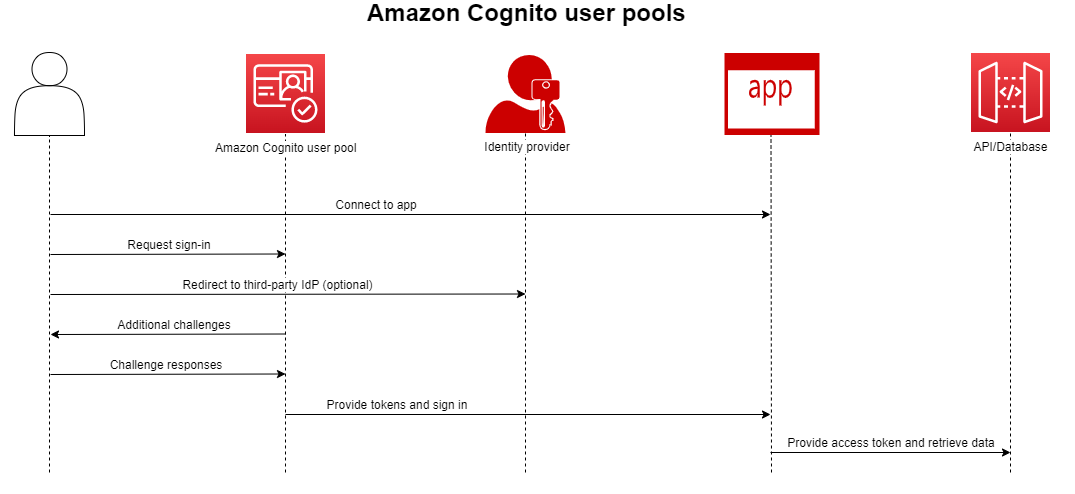
\includegraphics[width=.75\textwidth]{imagenes/ac_user_pool.png}
\caption{Grupo de Usuarios de Amazon Cognito diagrama de funcionamiento}
\end{figure}

\noindent Sirve para crear un grupo de usuarios cuando quiera autenticar y autorizar a los usuarios a la aplicación o la API. Los grupos de usuarios son un directorio de usuarios con funciones de creación, administración y autenticación de usuarios automáticas e impulsadas por el administrador. 
Los grupos de usuarios no requieren la integración con un grupo de identidades. Desde un grupo de usuarios, puede emitir JSON Web Token (JWT) autenticados directamente a una aplicación, un servidor web o una API.


\noindent Un grupo de usuarios de Amazon Cognito es un directorio de usuarios. Con un grupo de usuarios, los usuarios pueden iniciar sesión en su aplicación web o móvil por medio de Amazon Cognito o federarse mediante un IdP de terceros. Los usuarios federados y locales tienen un perfil de usuario en el grupo de usuarios.
Los grupos de usuarios de Amazon Cognito aceptan tokens y afirmaciones de IdP de terceros y recopilan los atributos de los usuarios en un JWT(JSON Web Token) que emite a la aplicación. Puede estandarizar la aplicación en un conjunto de JWT mientras Amazon Cognito gestiona las interacciones con los IdP y asigna las reclamaciones a un formato de token central. 

\subsubsection{Grupos de Identidades}

\begin{figure}[h]
\centering
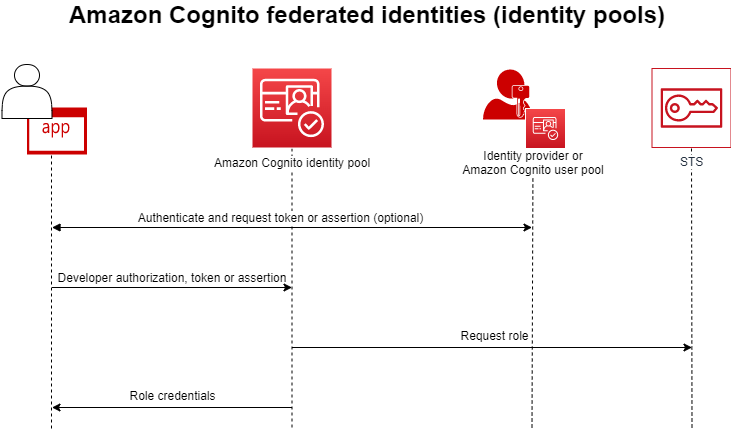
\includegraphics[width=.75\textwidth]{imagenes/ac_fed_pool.png}
\caption{Grupo de Usuarios de Amazon Cognito diagrama de funcionamiento}
\end{figure}

Configurar un grupo de identidades de Amazon Cognito cuando desee autorizar a los usuarios autenticados o anónimos a acceder a los recursos de AWS. Un grupo de identidades emite credenciales de AWS para que la aplicación proporcione recursos a los usuarios. Puede autenticar a los usuarios con un proveedor de identidades de confianza, como un grupo de usuarios. También puede emitir, opcionalmente, credenciales para los usuarios invitados. Los grupos de identidades utilizan un control de acceso basado en roles y atributos para administrar la autorización de los usuarios para acceder a los recursos de AWS.

Se utiliza Amazon Cognito para autenticar al usuario y, a continuación, concederle acceso a un Servicio de AWS.
\begin{enumerate}
\item El usuario de la aplicación inicia sesión a través de un grupo de usuarios y recibe los tokens de OAuth 2.0.
\item La aplicación intercambia un token de grupo de usuarios por un grupo de identidades para obtener credenciales de AWS temporales que puede usar con las API de AWS y la AWS Command Line Interface (AWS CLI).
\item La aplicación asigna la sesión de credenciales al usuario y proporciona acceso autorizado a Servicios de AWS como Amazon S3 y Amazon DynamoDB.
\end{enumerate}

En Amazon Cognito, la obligación de seguridad de la nube del modelo de responsabilidad compartida cumple con SOC 1-3, PCI DSS, ISO 27001 e HIPAA-BAA. Puede diseñar la seguridad en la nube en Amazon Cognito para que cumpla con SOC1-3, ISO 27001 e HIPAA-BAA, pero no con DSS de PCI. 


\noindent Un grupo de identidades es un conjunto de identificadores o identidades únicas que se asignan a los usuarios o invitados y se autoriza a recibir credenciales temporales de AWS. Al presentar una prueba de autenticación en un grupo de identidades en forma de afirmaciones fiables de un proveedor de identidades sociales (IdP) de SAML 2.0, OpenID Connect (OIDC) u OAuth 2.0, se asocia al usuario con una identidad del grupo de identidades. El token que el grupo de identidades crea para la identidad puede recuperar las credenciales de sesión temporales de AWS Security Token Service (AWS STS).

Para complementar las identidades autenticadas, también se puede configurar un grupo de identidades para autorizar el acceso de AWS sin autenticación de IdP. Puede ofrecer su propia prueba de autenticación personalizada o no tener autenticación. Puede conceder credenciales de AWS temporales a cualquier usuario de la aplicación que las solicite, con identidades no autenticadas.

\subsubsection{Control de Acceso con Base en Roles}
Cuando el usuario pasa las reclamaciones al grupo de identidades, Amazon Cognito elige el rol de IAM que solicita. Para personalizar los permisos del rol según las necesidades, se aplican las políticas de IAM a cada rol. Amazon Cognito puede solicitar un rol predeterminado, un rol basado en reglas que consultan las reclamaciones del usuario o un rol basado en la suscripción al grupo del usuario en un grupo de usuarios. También puede configurar la política de confianza de roles para que IAM confíe solo en el grupo de identidades para generar sesiones temporales\cite{129}.


\subsection{AWS Identity and Access Management}

AWS Identity and Access Management (IAM) es un servicio web que ayuda a controlar de forma segura el acceso a los recursos de AWS. Con IAM, se puede administrar de forma centralizada los permisos que controlan a qué recursos de AWS pueden acceder los usuarios. Se utiliza IAM; para controlar quién está autenticado (ha iniciado sesión) y autorizado (tiene permisos) para utilizar recursos.

Cuando se crea una Cuenta de AWS, se comienza con una identidad de inicio de sesión que tiene acceso completo a todos los recursos y Servicios de AWS de la cuenta. Esta identidad recibe el nombre de usuario raíz de la Cuenta de AWS y se accede a ella iniciando sesión con el email y la contraseña que utilizó para crear la cuenta. Se recomienda no utilizar la cuenta raíz para hacer actividades cotidianas\cite{130}.

Los 2 servicios anteriores únicamente son para autenticación lo cual es una herramienta muy importante ya que los datos que vamos a almacenar, aunque no sean confidenciales, sí son muy importantes y servirán para los análisis profesionales de los biólogos; y es destacable la forma de autenticación y verificación de las personas que se van a encargar del almacenamiento de los datos (nosotros mismos contaremos con los roles de administradores), ya que nosotros mismos nos encargaremos de darle seguridad e integridad a los datos para que no tengan vulnerabilidades los accesos y no entren intrusos a la información.

\subsection{Amazon Lambda}

AWS Lambda es un servicio informático que permite ejecutar código sin aprovisionar ni administrar servidores. Con Lambda, lo único que tiene que hacer es suministrar el código en uno de los tiempos de ejecución de lenguaje compatibles con Lambda \cite{131}.

Con el servicio de lambda podemos automatizar el proceso de limpieza de datos y el propio almacenamiento en la base de datos que vamos a utilizar, y podemos utilizar diferentes lenguajes de programación como Java o Python para procesar los datos.

\subsection{Amazon Simple Storage Service (Amazon S3)}

Amazon Simple Storage Service (Amazon S3) es un servicio de almacenamiento de objetos que ofrece escalabilidad, disponibilidad de datos, seguridad y rendimiento, se utiliza Amazon S3 para almacenar y proteger cualquier cantidad de datos para diversos casos de uso, tales como lagos de datos, sitios web, aplicaciones móviles, copia de seguridad y restauración, archivado, aplicaciones empresariales, dispositivos IoT y análisis de big data.

Amazon S3 proporciona funciones de gestión para que pueda optimizar, organizar y configurar el acceso a los datos almacenados.



\begin{figure}[hbtp]
\centering
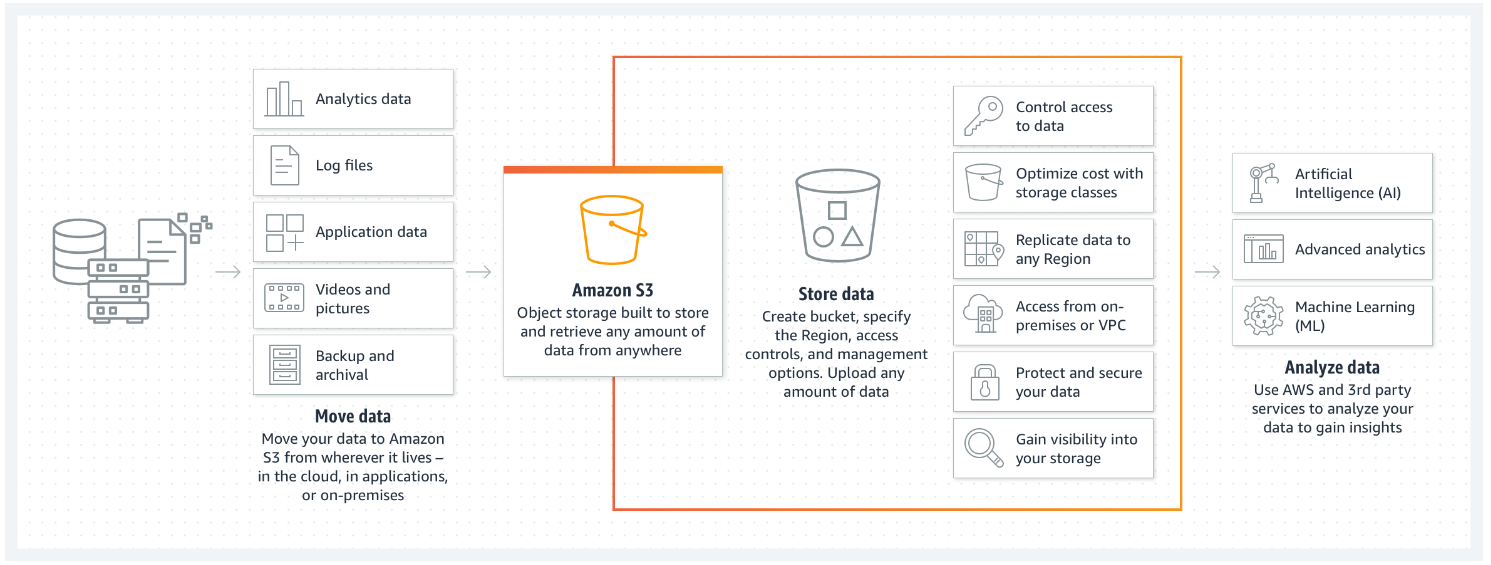
\includegraphics[width=\textwidth]{imagenes/s3.png}
\caption{Traslado de los datos a Amazon S3, administración de los datos almacenados en Amazon S3 y análisis de los datos con otros servicios de AWS. }
\end{figure}

El diagrama muestra cómo trasladar los datos a Amazon S3, administrar los datos almacenados en Amazon S3 y analizar los datos con otros servicios. Se muestran tres secciones de izquierda a derecha \cite{132}.

Amazon S3 ofrece varios tipos de almacenamiento diseñados para distintos casos de uso. Por ejemplo, puede almacenar datos de producción críticos en S3 Standard para obtener acceso frecuente, ahorrar costos al almacenar datos a los que se accede con poca frecuencia en S3 Standard-IA o S3 One Zone-IA, y archivar datos con los costos más bajos en S3 Glacier Instant Retrieval, S3 Glacier Flexible Retrieval y S3 Glacier Deep Archive.

También, se pueden instanciar páginas web en el servicio de de S3, por lo que nos será útil para cuando diseñemos la página web para visualización y acceso a los datos de usuarios que tengan permiso y acceso a ellos.

\subsection{Amazon DynamoDB}
Amazon DynamoDB es un servicio de base de datos NoSQL totalmente administrado que ofrece un rendimiento rápido y predecible, así como una perfecta escalabilidad. Permite delegar las cargas administrativas que supone tener que utilizar y escalar bases de datos distribuidas, para que no tengamos que preocuparnos del aprovisionamiento, la instalación ni la configuración del hardware, ni tampoco de las tareas de replicación, aplicación de parches de software o escalado de clústeres. DynamoDB también ofrece el cifrado en reposo, que elimina la carga y la complejidad operativa que conlleva la protección de información confidencial. 

Podemos crear tablas de base de datos capaces de almacenar y recuperar cualquier cantidad de datos, así como de atender cualquier nivel de tráfico de solicitudes. Se puede escalar la capacidad de rendimiento de las tablas para aumentarla o reducirla sin tiempos de inactividad ni reducción del desempeño.

\begin{figure}[hbtp]
\centering
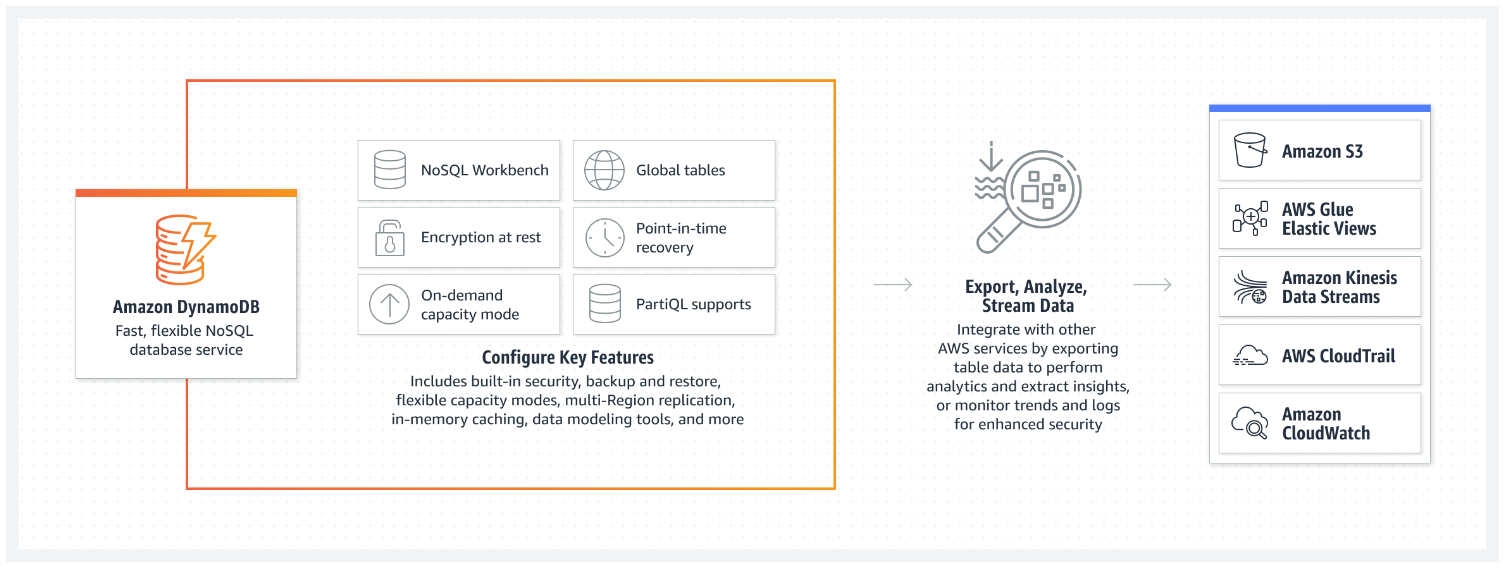
\includegraphics[width=\textwidth]{imagenes/dynamodb.png}
\caption{Características principales de Amazon DynamoDB y las integraciones con otros servicios de AWS}
\end{figure}


En el diagrama se muestran las características principales de Amazon DynamoDB y las integraciones con otros servicios de AWS. Se muestran tres secciones de izquierda a derecha.

Las características de importación y exportación de DynamoDB ayudan a mover, transformar y copiar cuentas de tablas de DynamoDB, o AWS. Se puede importar desde sus orígenes de S3 y puede exportar los datos de sus tablas de DynamoDB a Amazon S3 y utilizar servicios de AWS como Athena, Amazon SageMaker y AWS Lake Formation que son servicios que se pueden considerar introducir en algún momento para analizar los datos y extraer información procesable. También se puede importar datos directamente a nuevas tablas de DynamoDB para crear nuevas aplicaciones con un rendimiento de un milisegundo a escala, facilitar el uso compartido de datos entre tablas y cuentas, y simplificar sus planes de recuperación de desastres y continuidad empresarial \cite{133}.

\subsection{Amazon QuickSight}
Amazon QuickSight es una herramienta que nos ayudará a crear presentaciones gráficas sobre los datos que obtengamos, podremos utilizar diversas gráficas que nos ayudarán a una mejor visualización de los datos, serán más entendibles que simple texto plano y serán más amigables de entregar en reportes de análisis de datos.

Lo que estaremos usando serán estos servicios de almacenamiento, gestión y seguridad de datos. Es muy importante la conexión e integración de estos servicios ya que cada uno realizará una tarea en específico para lograr los objetivos de análisis de la especie a analizar.

El siguiente esquema es una representación gráfica de lo que vamos a hacer en el proyecto.

\begin{figure}[h]
\centering
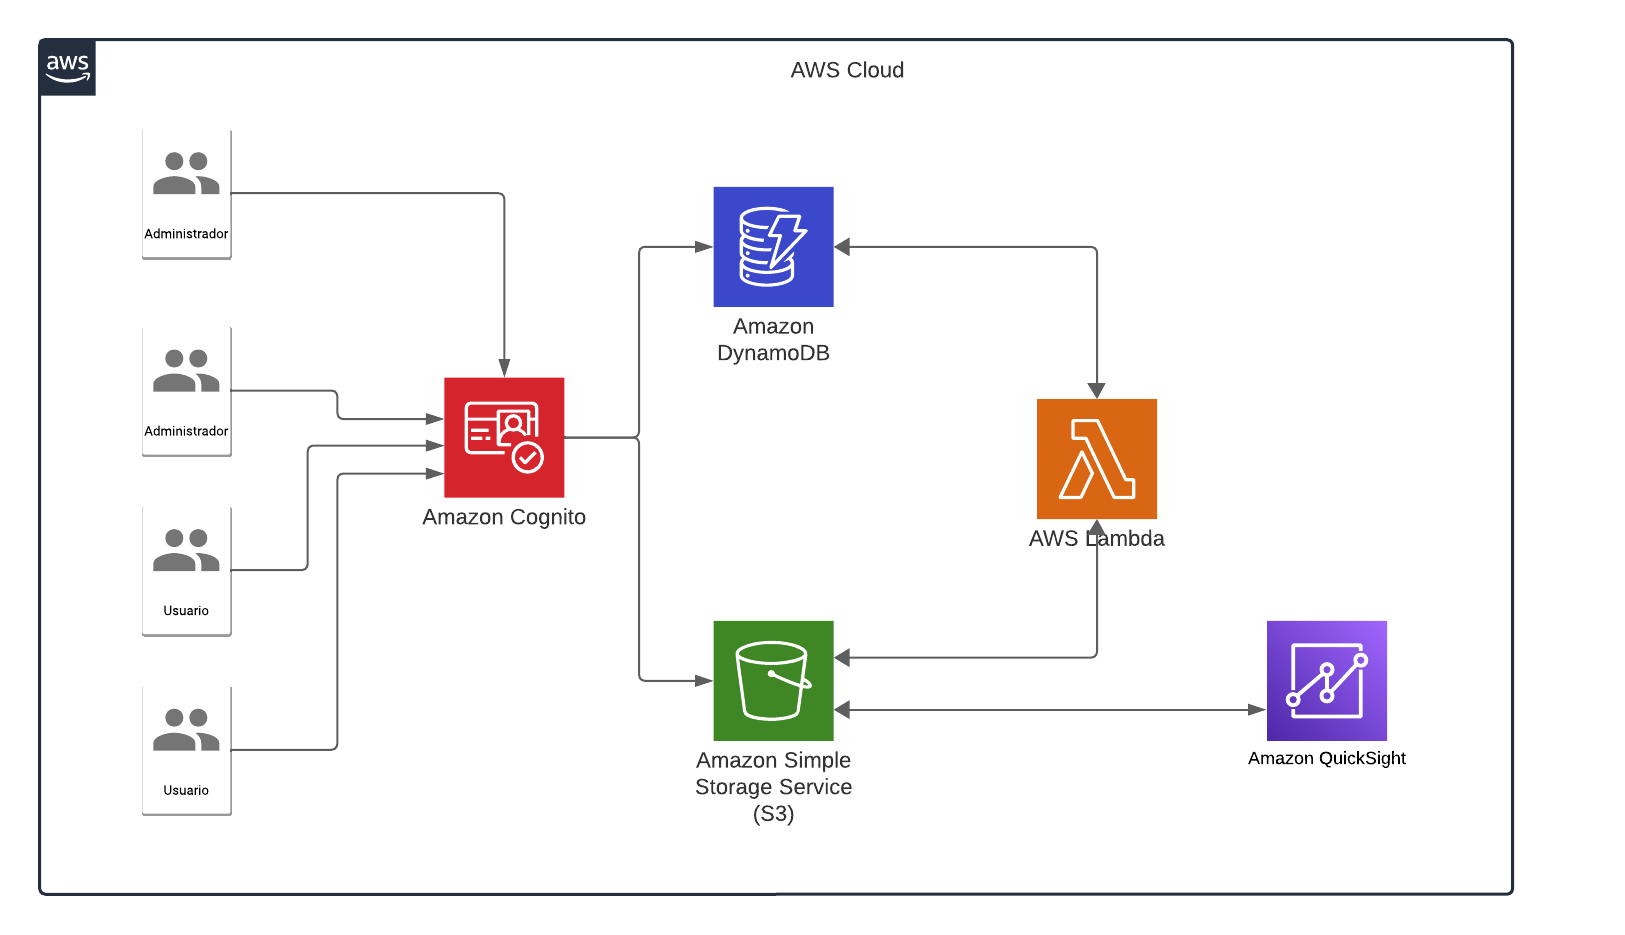
\includegraphics[width=\textwidth]{imagenes/diagrama.png}
\caption{Diagrama de bloques de los servicios que se consideran para el desarrollo del proyecto.}
\end{figure}

Habrán 2 administradores que serán los alumnos que desarrollarán el proyecto y tendrán todos los permisos, contaremos con 2 usuarios (depende como evolucione el proyecto se irán incluyendo más usuarios) los cuales no contarán con todos los permisos de escritura y únicamente contarán con los permisos de visualización de los datos, y estos 2 usuarios serán los asesores del proyecto. Usaremos el servicio de Amazon Cognito para la validación de identidades de los usuarios (se aplicará a los usuarios administradores y los usuarios normales), posteriormente usaremos 2 servicios de almacenamiento, el servicio de S3 lo usaremos como almacenamiento de todos los datos que involucran al proyecto, tales son archivos de video, imágen, audio, texto plano, gráficos, entre otros tipos de archivos, el servicio de DynamoDB será ocupado como la base de datos NoSQL en la cuál vamos a crear nuestras tablas NoSQL donde organizaremos nuestros archivos.

Es muy importante hacer la diferencia entre los servicios DynamoDB y S3, DynamoDB es una base de datos que se almacenan en caché y únicamente crearemos tablas NoSQL para identificación de archivos, por lo que para almacenar los datos necesitamos el servicio de S3 que será el lugar de almacenamiento de todos los archivos descritos anteriormente y también almacenaremos copias de seguridad y las propias tablas que generamos en DynamoDB.

Usaremos el servicio de Lambda que estará vinculado a los servicios de S3 y DynamoDB para procesar archivos. Con lo de procesar los datos nos referimos a la limpieza de los datos y almacenamiento automático de los datos. Ya que el servicio de Lambda nos ayuda a crear funciones que nos permitirán procesar los datos con diferentes lenguajes de programación, entre ellos podemos usar Java y Python.

El servicio de QuickSight únicamente lo tomamos para visualización de los datos, ya que es muy necesario interpretar de forma correcta los datos obtenidos por nosotros y crear gráficas o recursos visuales que nos ayuden a entender de forma más sencilla los datos limpios, aunque este servicio lo podemos reemplazar por el propio AWS Lambda o algún programa de manipulación de datos local como PowerBI u otros en línea como Tableau que se pueden colocar nuestros resultados en línea para consulta de terceros (esto es opcional y dependerá de los permisos de publicación de datos con las vinculaciones que tengamos con los biólogos).

\newpage
\section{Creación del Dominio en la Nube}
El dominio en la nube se elaboró con una cuenta de los alumnos que están desarrollando el proyecto y contiene la siguiente información.


\begin{figure}[h]
\centering
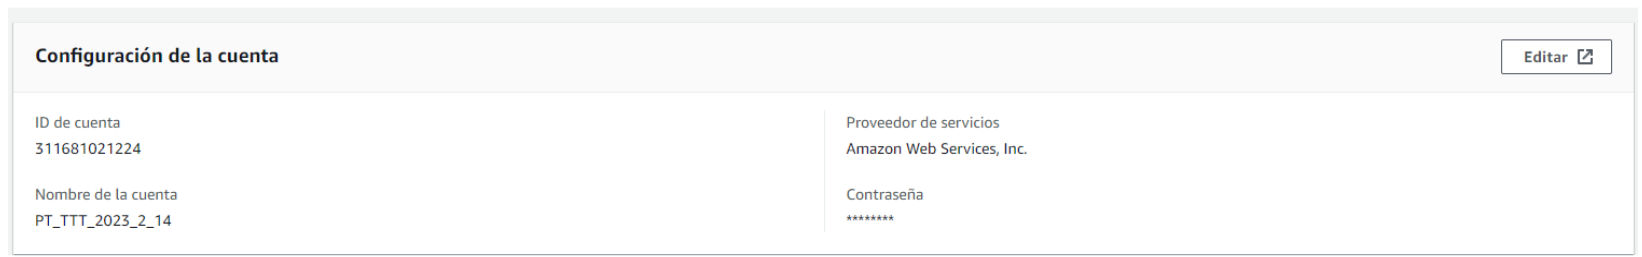
\includegraphics[width=\textwidth]{imagenes/cuenta.png}
\caption{Características del dominio en la nube.}
\end{figure}
\newpage

Ya creado el dominio, podemos observar la página de inicio y podemos empezar a usar los servicios; Es importante estar inspeccionando los precios de los servicios para estar informados sobre los movimientos que vamos haciendo y saber cuánto dinero es necesario pagar al final de la fecha de facturación.

\begin{figure}[h]
\centering
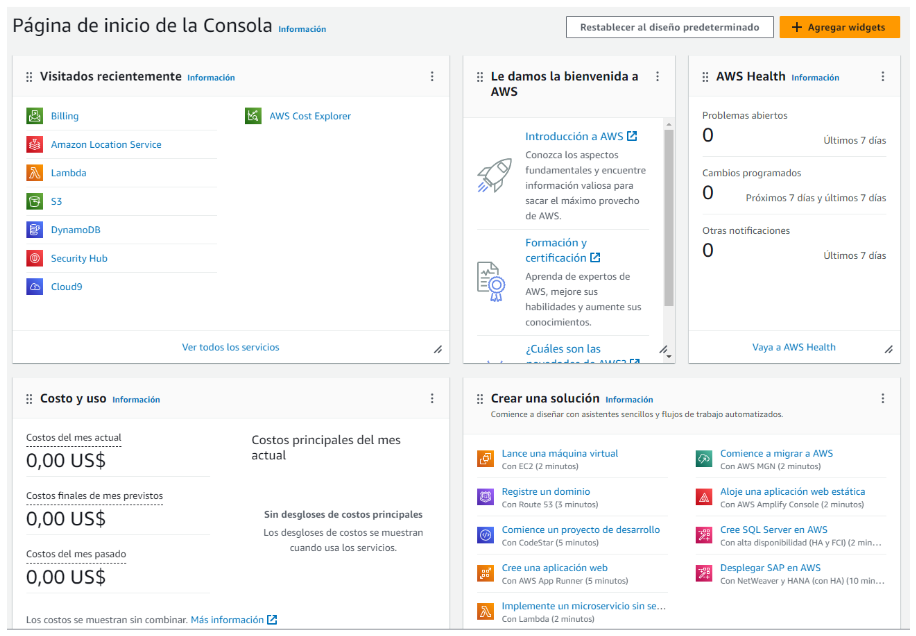
\includegraphics[width=0.8\textwidth]{imagenes/pag_principal.png}
\caption{Visualización de la página principal al iniciar sesión en AWS}
\end{figure}





\chapter{Implementación del sistema}
%
\section{Implementación de los drones}
Para el proceso de documentación del armado de los drones, se tiene en cuenta los siguientes elementos : 
\begin{itemize}[itemsep=0pt,parsep=0pt,topsep=0pt,partopsep=0pt]
  \item Chasis de Kit: S500
  \item Propelas: Nylon 1045
  \item Motor sin escobillas: 2212 920KV
  \item Controladoras de Velocidad: RC Brushless (ESC)
  \item Power Distribution Board (PDB) y Power Module: Apm2.8 2.6 2.52
  \item Batería LiPo 3S de 11.1V - 5000mAh
  \item Controladora de vuelo: Pixhawk 2.4.8
  \item Sistema de GPS: HERE+
  \item Sistema de Telemetría NRF24L01
  \item Transceptor De Telemetría Personalizado: NRF24L01
  \item RaspBerry Pi4
  \item Xiangtat Flysky FS-i6X 2.4GHz 10CH AFHDS 2A RC Transmisor TX con receptor iA6B (Radio transmisor para control manual)
\end{itemize}

\noindent Comenzando con el armado del dron, se utilizará el Chasis S500, el cual viene con los siguientes elementos:
\begin{itemize}[itemsep=3pt,parsep=0pt,topsep=0pt,partopsep=0pt]
  \item Placa central PCB con punto de soldadura
  \item Tubos de fibra de carbono de 16 mm de diámetro con una altura de 250 mm
  \item Tubos de fibra de carbono de 10 mm de diámetro con longitud de 250 mm para la base
  \item Tubos de esponja anti salto
  \item Brazos DJI S800 EVO con 6 agujeros para colocar motores
\end{itemize}
\begin{figure}[H]
    \centering
    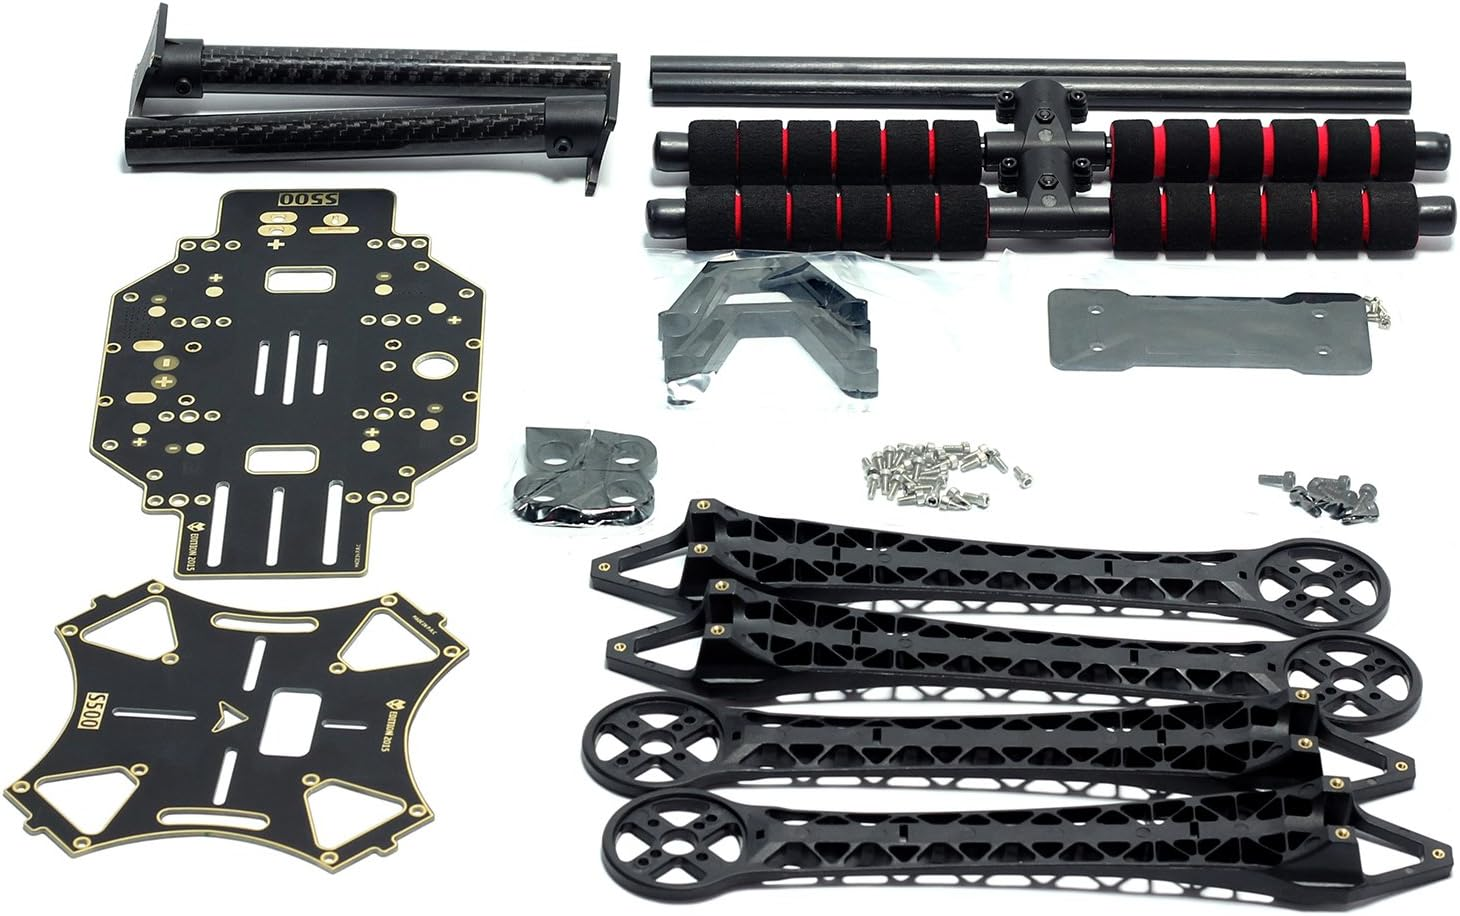
\includegraphics[width=0.6\textwidth]{imagenes/componenteskit.png}
    \caption{Componentes del Kit S500.}
    \label{fig:kitS500}
\end{figure}
El primer paso para el armado del chasis S500 es para el tren de aterrizaje. Se arma tal como se muestra en la siguiente imagen:
\begin{figure}[H]
    \centering
    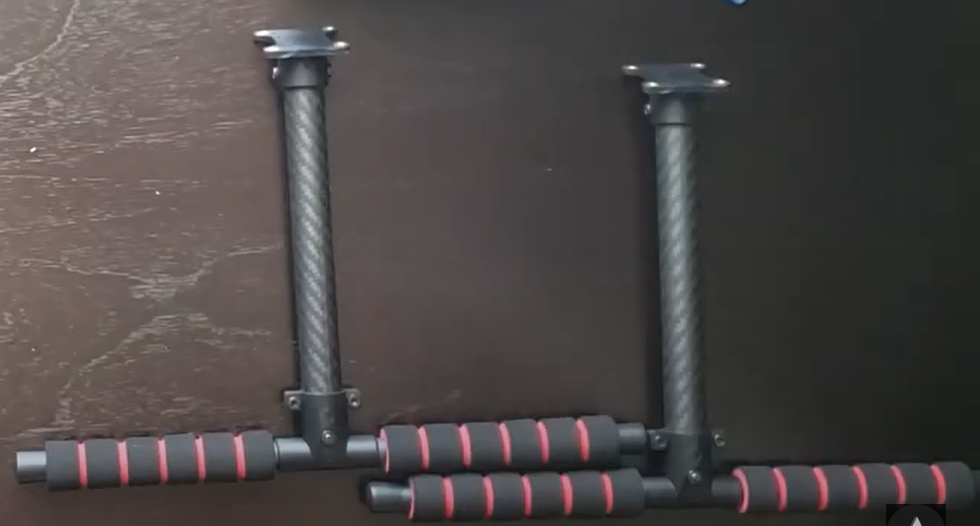
\includegraphics[width=0.7\textwidth]{imagenes/base-tren.png}
    \caption{Base para el tren de aterrizaje.}
    \label{fig:basetren}
\end{figure}

\noindent Se colocan los tubos de fibra de carbono para que formen la base del cuadricóptero. Se van a montar sobre la placa central para formar la base.
\begin{figure}[H]
    \centering
    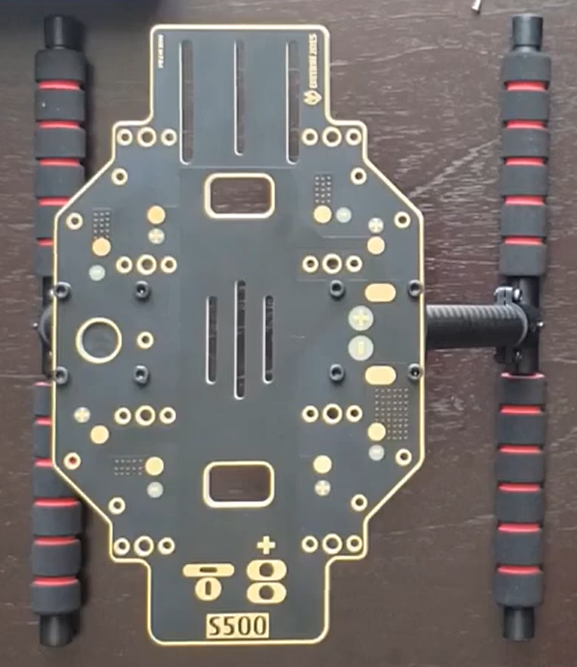
\includegraphics[width=0.45\textwidth]{imagenes/chasis-sobre-tren.png}
    \caption{Chasis montado sobre el tren de aterrizaje.}
    \label{fig:basetren}
\end{figure}
\noindent Cuando ya está la base armada, se procede al armado de los brazos de la placa superior que consta de los 4 brazos y la placa superior.

\begin{figure}[H]
    \centering
   {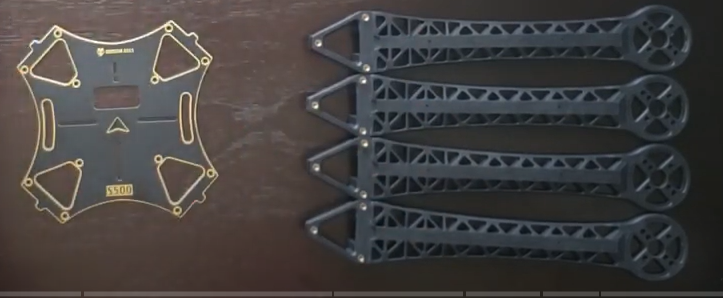
\includegraphics[width=0.7\textwidth]{imagenes/brazos.png}} 
    {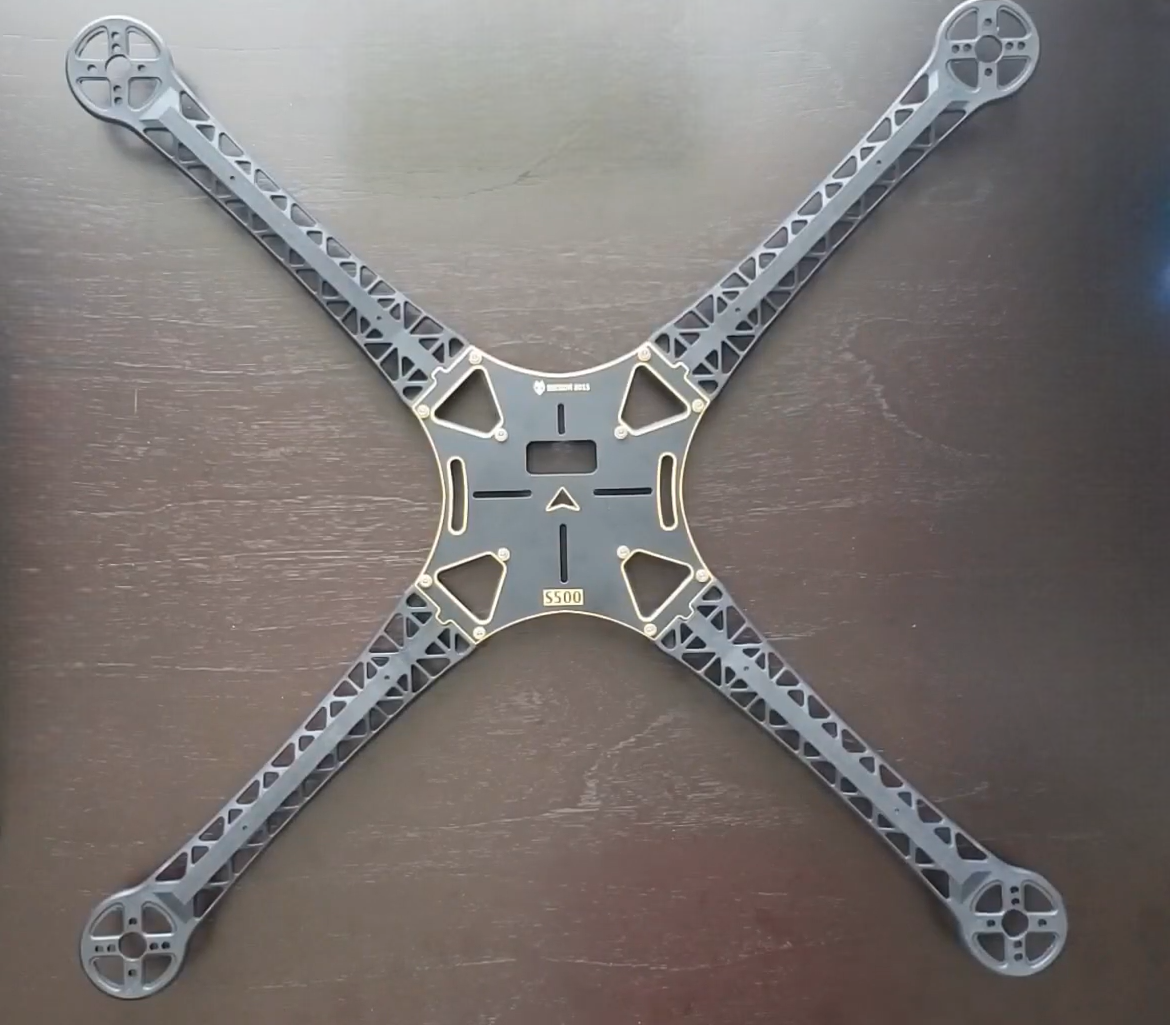
\includegraphics[width=0.7\linewidth]{imagenes/brazos-armados.png}}
    \caption{Base con 4 brazos para el armado de la placa superior.}
    \label{fig:lora-solo}
\end{figure}

\noindent Cuando la placa superior esté armada, se colocan los controladores de velocidad (ESC), los cuales debe tener en cuenta el sentido de giro de los motores y el diseño de las propelas como se muestra en la siguiente figura:

\begin{figure}[H]
    \centering
    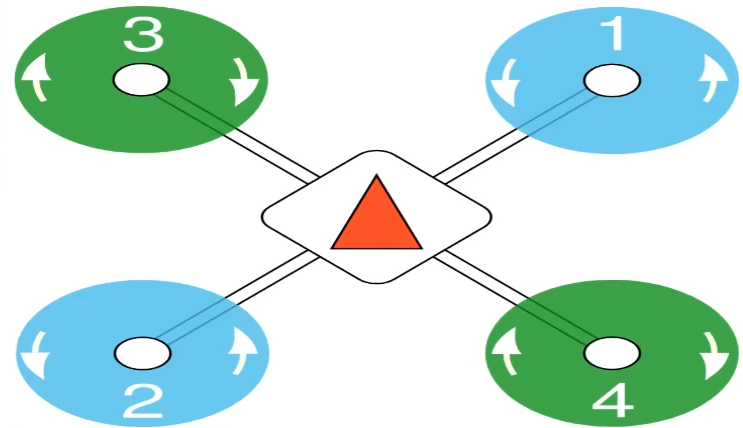
\includegraphics[width=0.5\textwidth]{imagenes/sentidodegiro.png}
    \caption{Sentido de giro de los motores.}
    \label{fig:basetren}
\end{figure}
\noindent Con esta consideración en los extremos se soldan los controladores de velocidad ESC con el tablero de distribución de energía (PDB) y el módulo de potencia.. El amperaje del ESC depende de la corriente que consumen los motores, siendo de 20\% más amperaje cómo mínimo (si el motor consume 10A, el ESC debe ser de 12A como mínimo).
\begin{figure}[H]
    \centering
    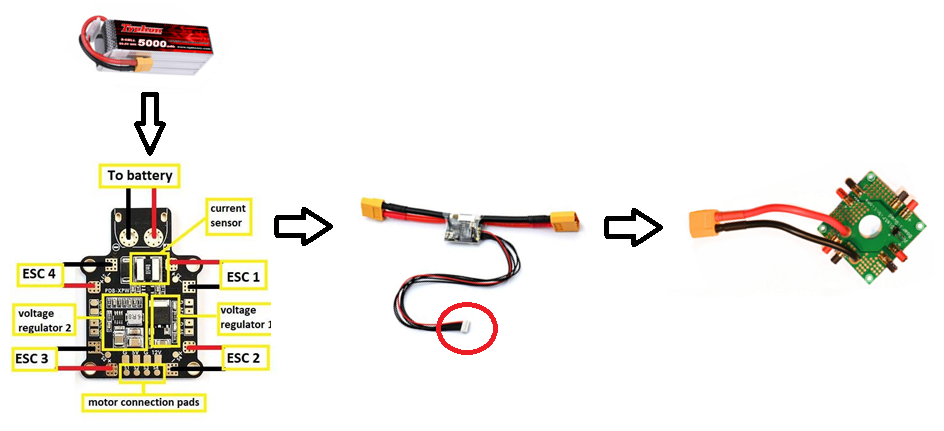
\includegraphics[width=\textwidth]{imagenes/componentes-potencia.png}
    \caption{Componentes de la parte de potencia del dron.}
    \label{fig:basetren}
\end{figure}
\newpage
\begin{figure}[H]
    \centering
    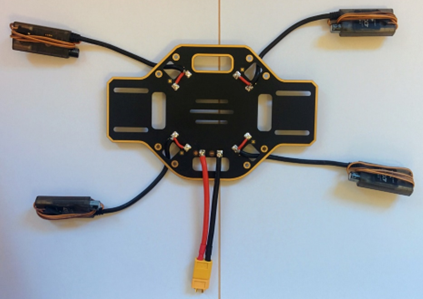
\includegraphics[width=0.7\textwidth, height=7cm]{imagenes/placa-esc.png}
    \caption{Placa superior con las ESC montadas y sin brazos.}
    \label{fig:basetren}
\end{figure}
\noindent Una vez teniendo el conjunto de las ESC y los módulos de distribución de potencia soldados, se procede a instalar los motores. Los motores utilizados son los motores sin escobillas: 2212 920KV que cuentan con las siguientes características.
\begin{itemize}
    \item Eficiencia máxima: 80\%
    \item Eficiencia de la corriente máxima: 4-10A ($>$ 75\%)
    \item Capacidad de corriente: 12A/60s
    \item Consumo de corriente sin carga a 10 V: 0.5A
    \item Eficiencia -MAX real: 4-10A ($>$ 75\%)
    \item RPM/V: 930 KV
    \item Diámetro del eje: 3.17mm
    \item Dimensiones: 28 x 28 x 39 mm
    \item Peso: 67g
\end{itemize}
\newpage
\begin{figure}[H]
    \centering
    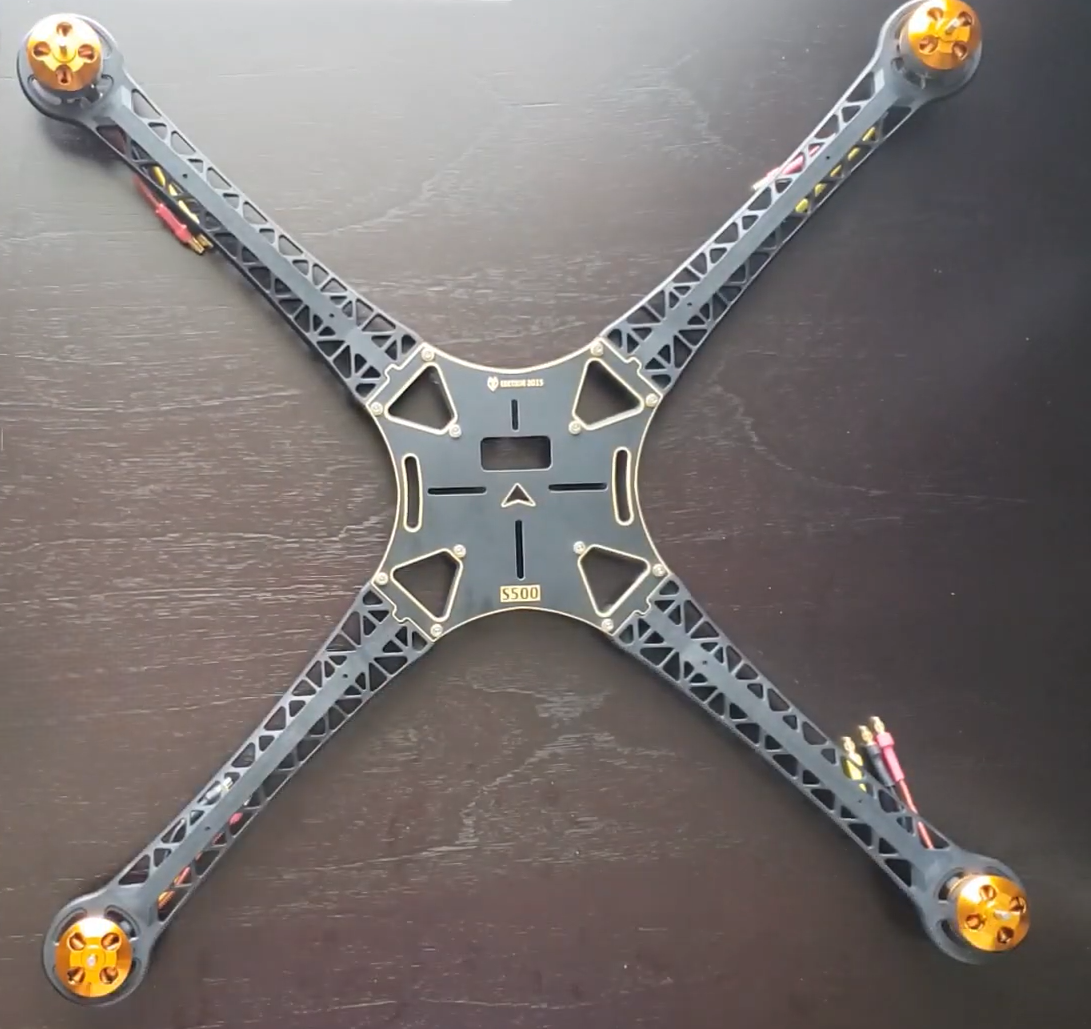
\includegraphics[width=0.5\textwidth]{imagenes/placa-motores.png}
    \caption{Placa superior con los motores montados.}
    \label{fig:basetren}
\end{figure}
\noindent Una vez ensambladas los componentes de ambas partes (la placa principal y la placa superior), únicamente hay que unir estos 2 conjuntos. Colocando la placa superior sobre la placa principal, utilizando los tornillos que ya vienen incluidos sobre el KIT S500. No hay que perder en cuenta las conexiones que se consideraron del sentido de rotación de los motores.
\begin{figure}[H]
    \centering
    {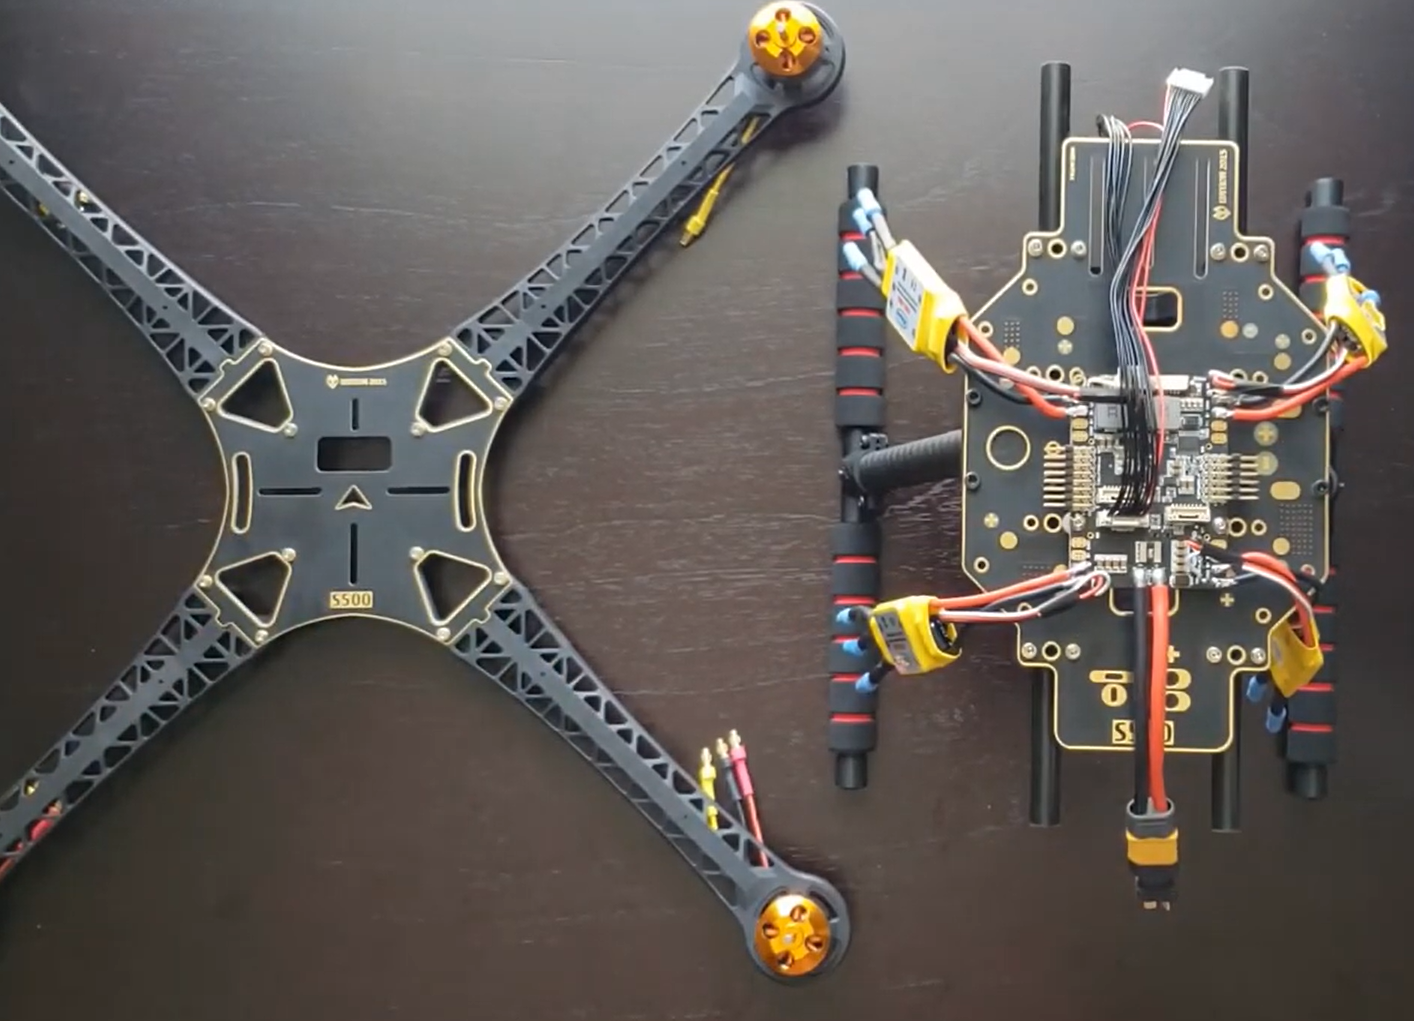
\includegraphics[width=0.5\linewidth]{imagenes/superior-inferior.png}}
    \caption{Montaje de la placa superior sobre la placa base (por partes).}
    \label{fig:lora-solo-parte1}
\end{figure}

\begin{figure}[H]
    \centering
    {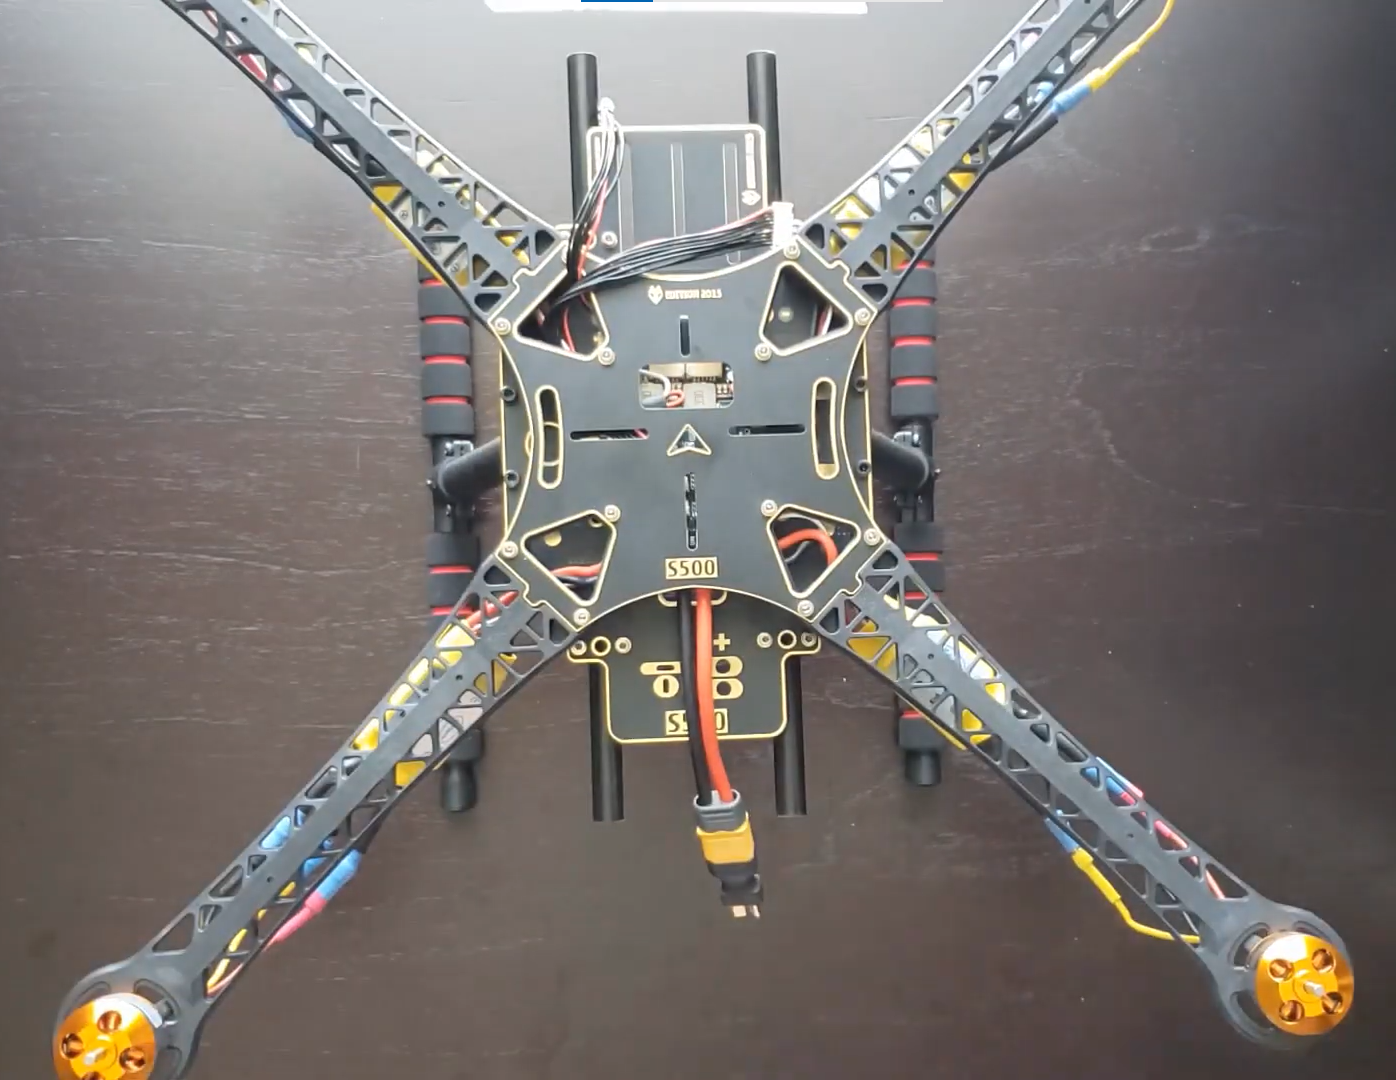
\includegraphics[width=0.5\linewidth]{imagenes/sup-inf-unidas.png}}
    \caption{Montaje de la placa superior sobre la placa base (armada).}
    \label{fig:lora-solo-parte2}
\end{figure}
\noindent Para finalizar el ensamblado básico del dron, se añade la computadora de vuelo Pixhawk 2.4.8 y el módulo GPS para el posicionamiento del dron.
Para el módulo GPS, debe estar separado mínimo 15 cm de la computadora de vuelo para no causar interferencia, por lo que se le coloca en un mástil que irá en la parte superior.
\begin{figure}[H]
    \centering
    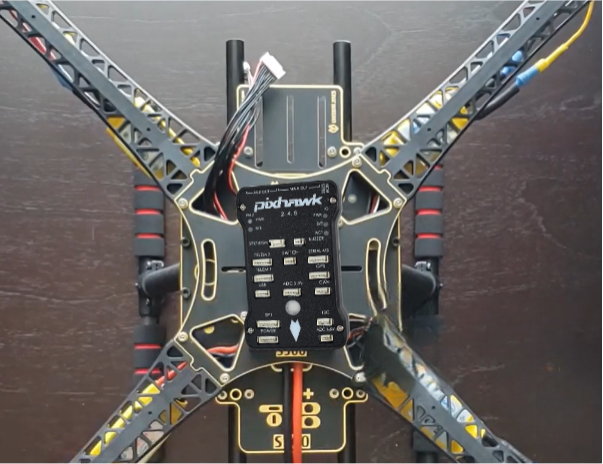
\includegraphics[width=0.5\textwidth]{imagenes/pix-montada.png}
    \caption{Montaje de la computadora de vuelo sobre la placa superior.}
\end{figure}
\begin{figure}[H]
    \begin{minipage}{\textwidth}
        \centering
        \begin{minipage}{\textwidth}
            \centering
            \subfigure[) Individualmente.]{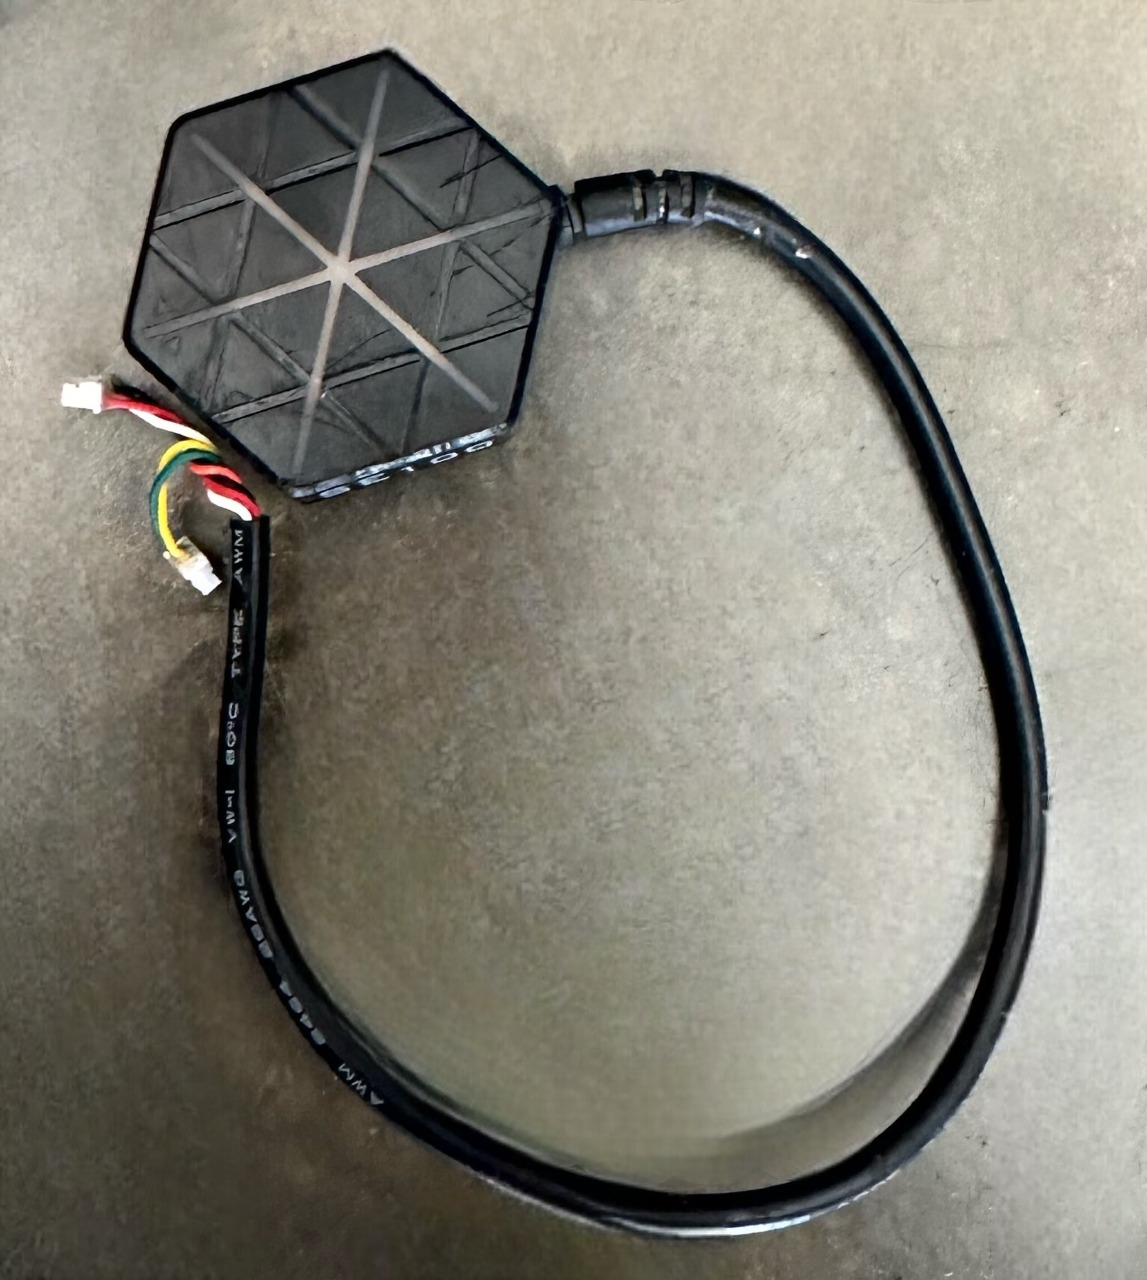
\includegraphics[width=0.3\textwidth]{imagenes/gps-sindron.jpeg}}\hspace{0.1\textwidth}
            \subfigure[) Mástil.]{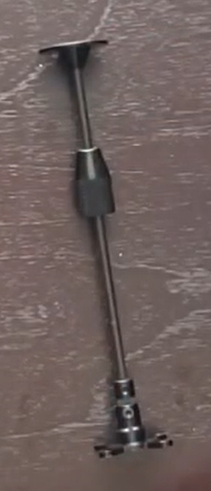
\includegraphics[width=0.15\textwidth]{imagenes/mastil.png}}
        \end{minipage}
    \end{minipage}
    
    \begin{minipage}{\textwidth}
        \centering
        \begin{minipage}{\textwidth}
            \centering
            \subfigure[)  Montado.]{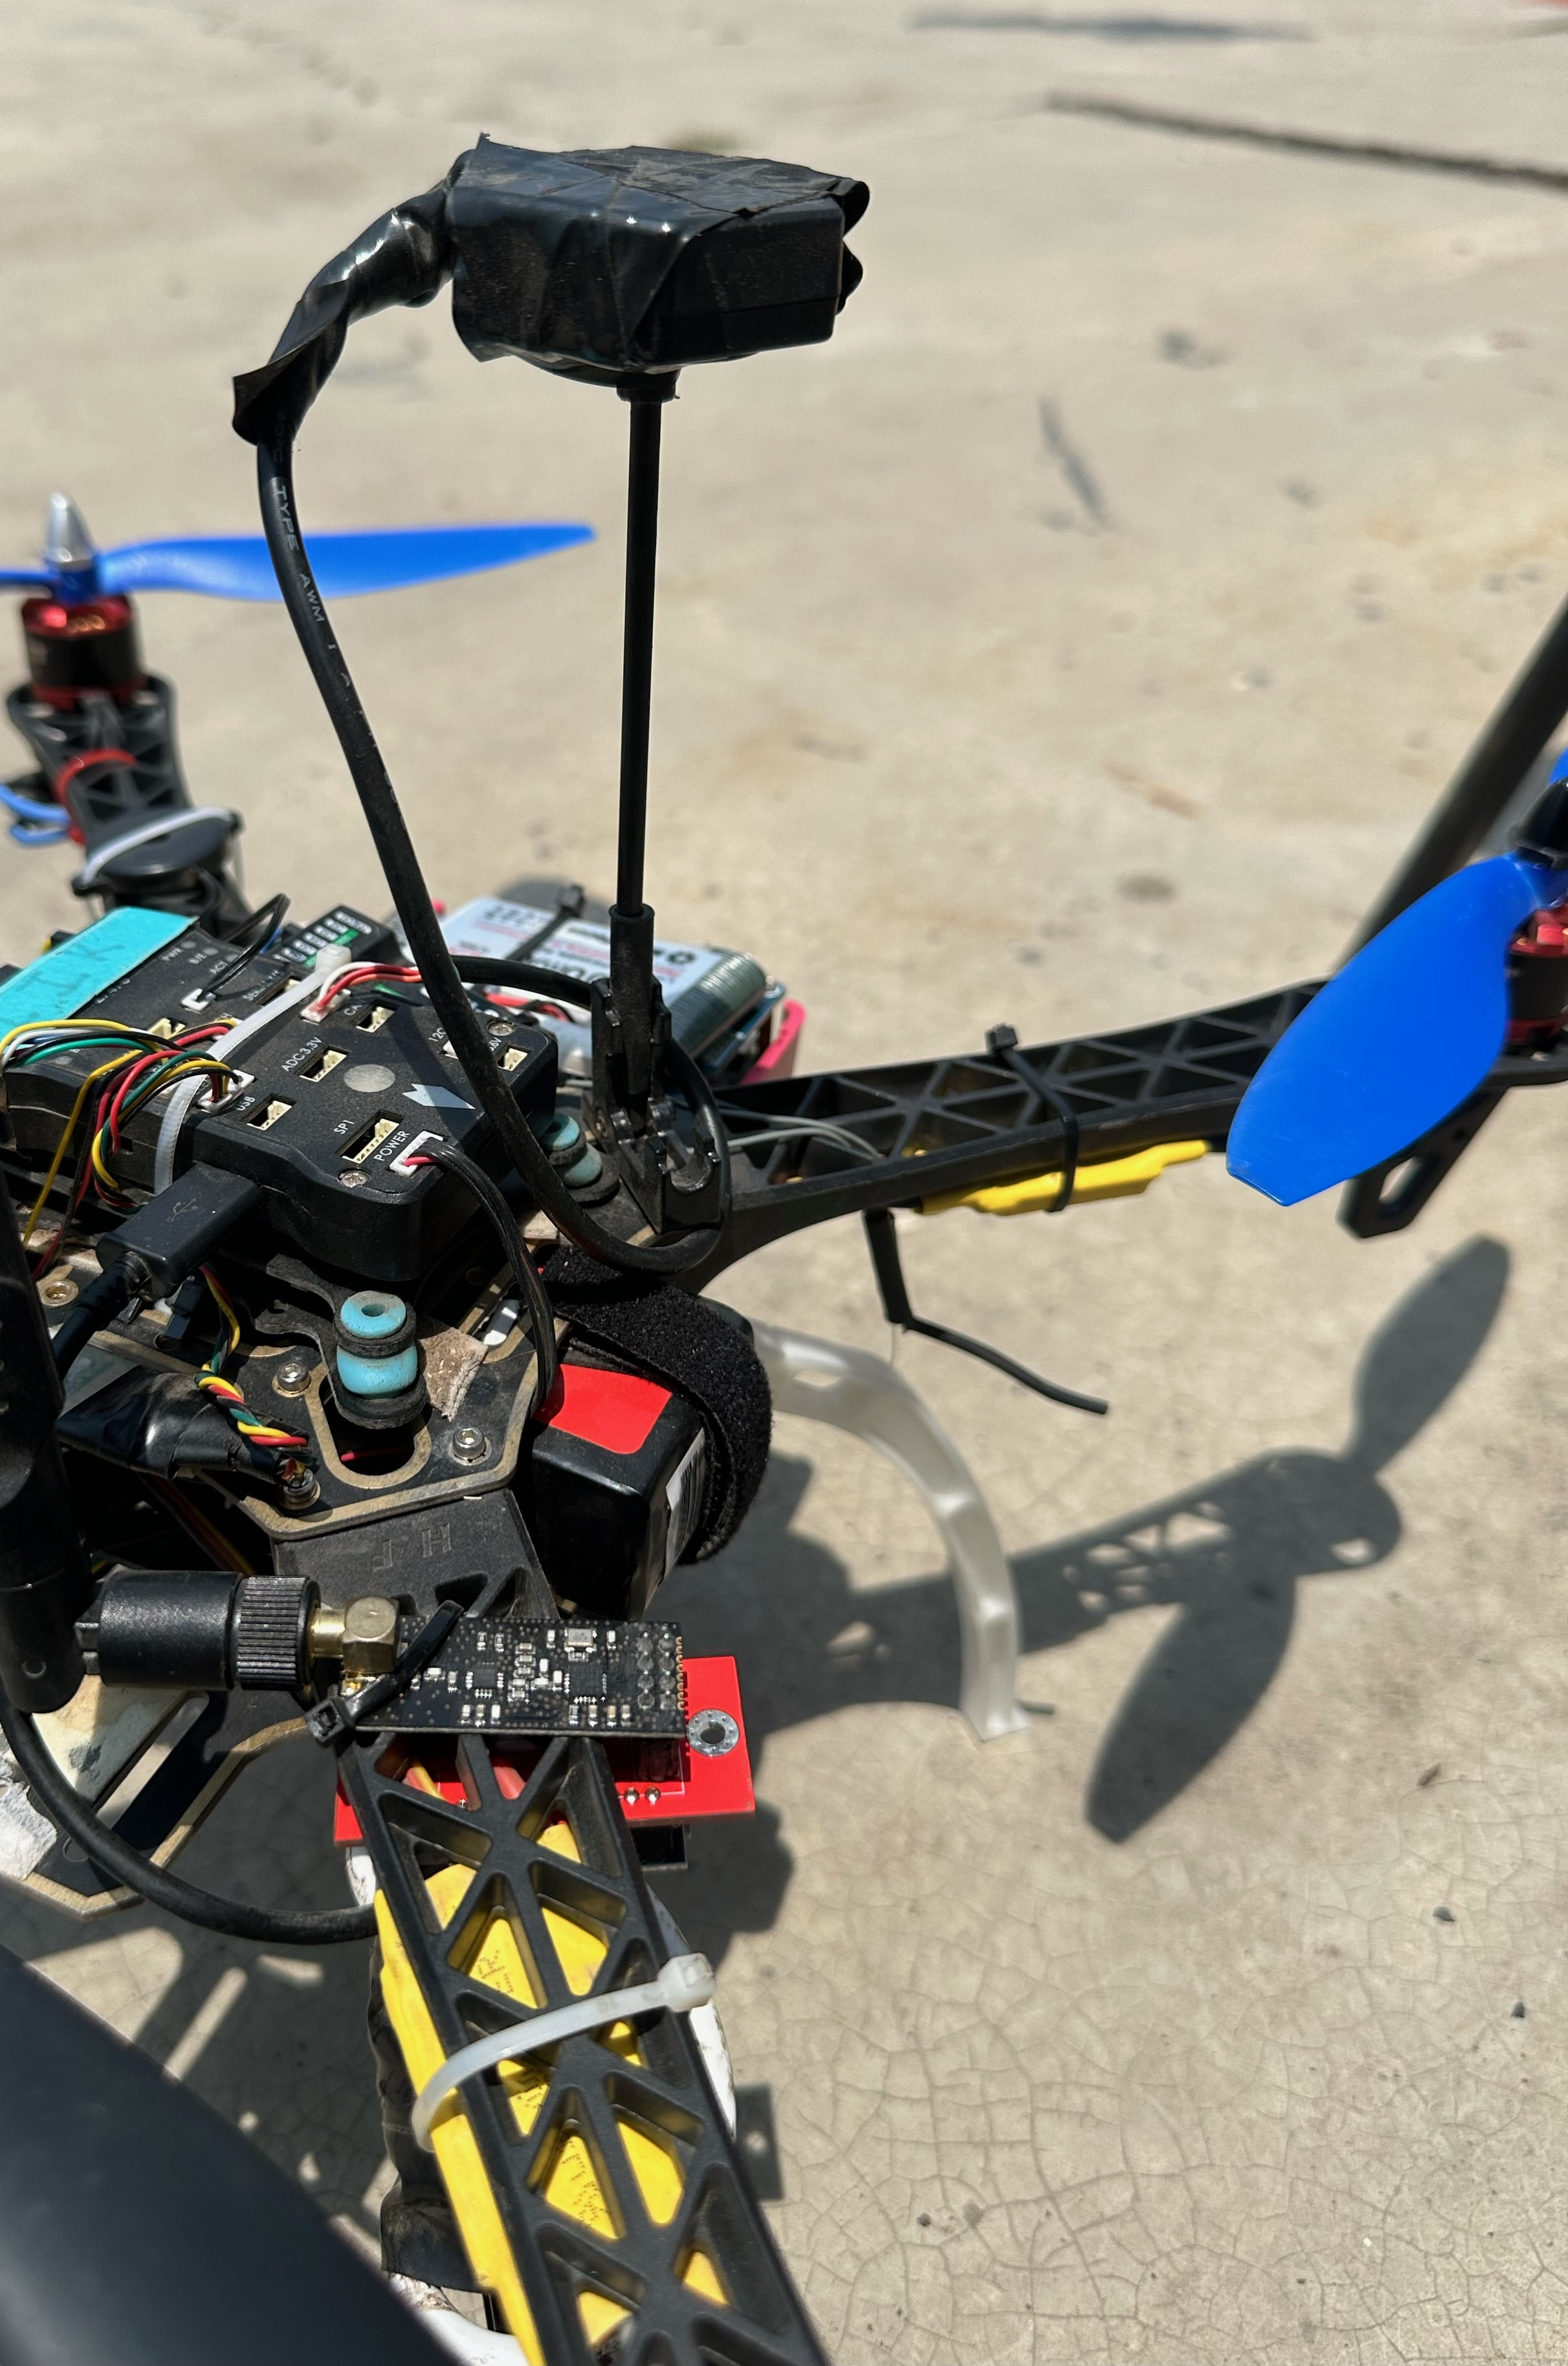
\includegraphics[width=0.35\textwidth]{imagenes/gps-montado.jpeg}}
        \end{minipage}
    \end{minipage}
    
    \caption{Montaje del GPS de vuelo sobre la placa superior.}
\end{figure}

La computadora de vuelo Pixhawk 2.4.8 cuenta con las siguientes características:
\begin{itemize}[itemsep=0pt, parsep=0pt, topsep=0pt]
    \item \textbf{Microprocesador}
    \begin{itemize}[label=o, itemsep=0pt, parsep=0pt, topsep=0pt, partopsep=0pt]
        \item Frecuencia: 168 MHZ, 256K RAM
        \item Coprocesador de copia de seguridad 32 STM32F103
    \end{itemize}
    \item \textbf{Sensor}
    \begin{itemize}[label=o, itemsep=0pt, parsep=0pt, topsep=0pt, partopsep=0pt]
        \item Giroscopio digital de 3 ejes L3GD20 16
        \item Acelerómetro de 3 ejes LSM303D 14/Magnetómetro
        \item Acelerómetro / magnetómetro MPU6000 de 6 ejes
        \item Barómetro de precisión MS5607
    \end{itemize}
    \item \textbf{Interfaz}
    \begin{itemize}[label=o, itemsep=0pt, parsep=0pt, topsep=0pt, partopsep=0pt]
        \item UART 1, 2 compatible con alto voltaje con control de flujo de hardware
        \item Entrada compatible con receptor de satélite Spektrum DSM / DSM2 / DSM-X
        \item Entradas y salidas compatibles con Futaba SBUS
        \item Entrada de señal PPM
        \item Entrada RSSI (PWM o voltaje) 
        \item I2C 
        \item SPI 
        \item 3.3 y entrada 6.6VADC 
        \item Interfaz micro USB externa
    \end{itemize}
\end{itemize}
\begin{figure}[H]
    \centering
    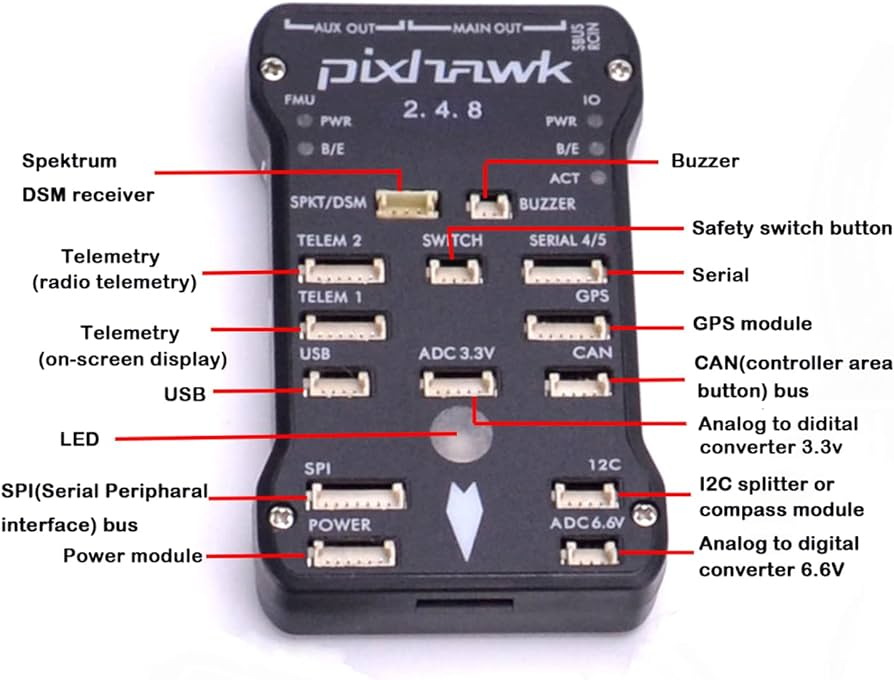
\includegraphics[width=0.6\textwidth, height=7cm]{imagenes/diagrama-pix.png}
    \caption{Diagrama de conexiones de la computadora de vuelo Pixhawk 2.4.8}
    \label{fig:basetren}
\end{figure}
\noindent Se utilizan las conexiones de POWER, las 2 de telemetría, el módulo GPS, el buzzer, el safety switch y la comunicación I2C, como se muestra en la siguiente figura:
\begin{figure}[H]
    \centering
    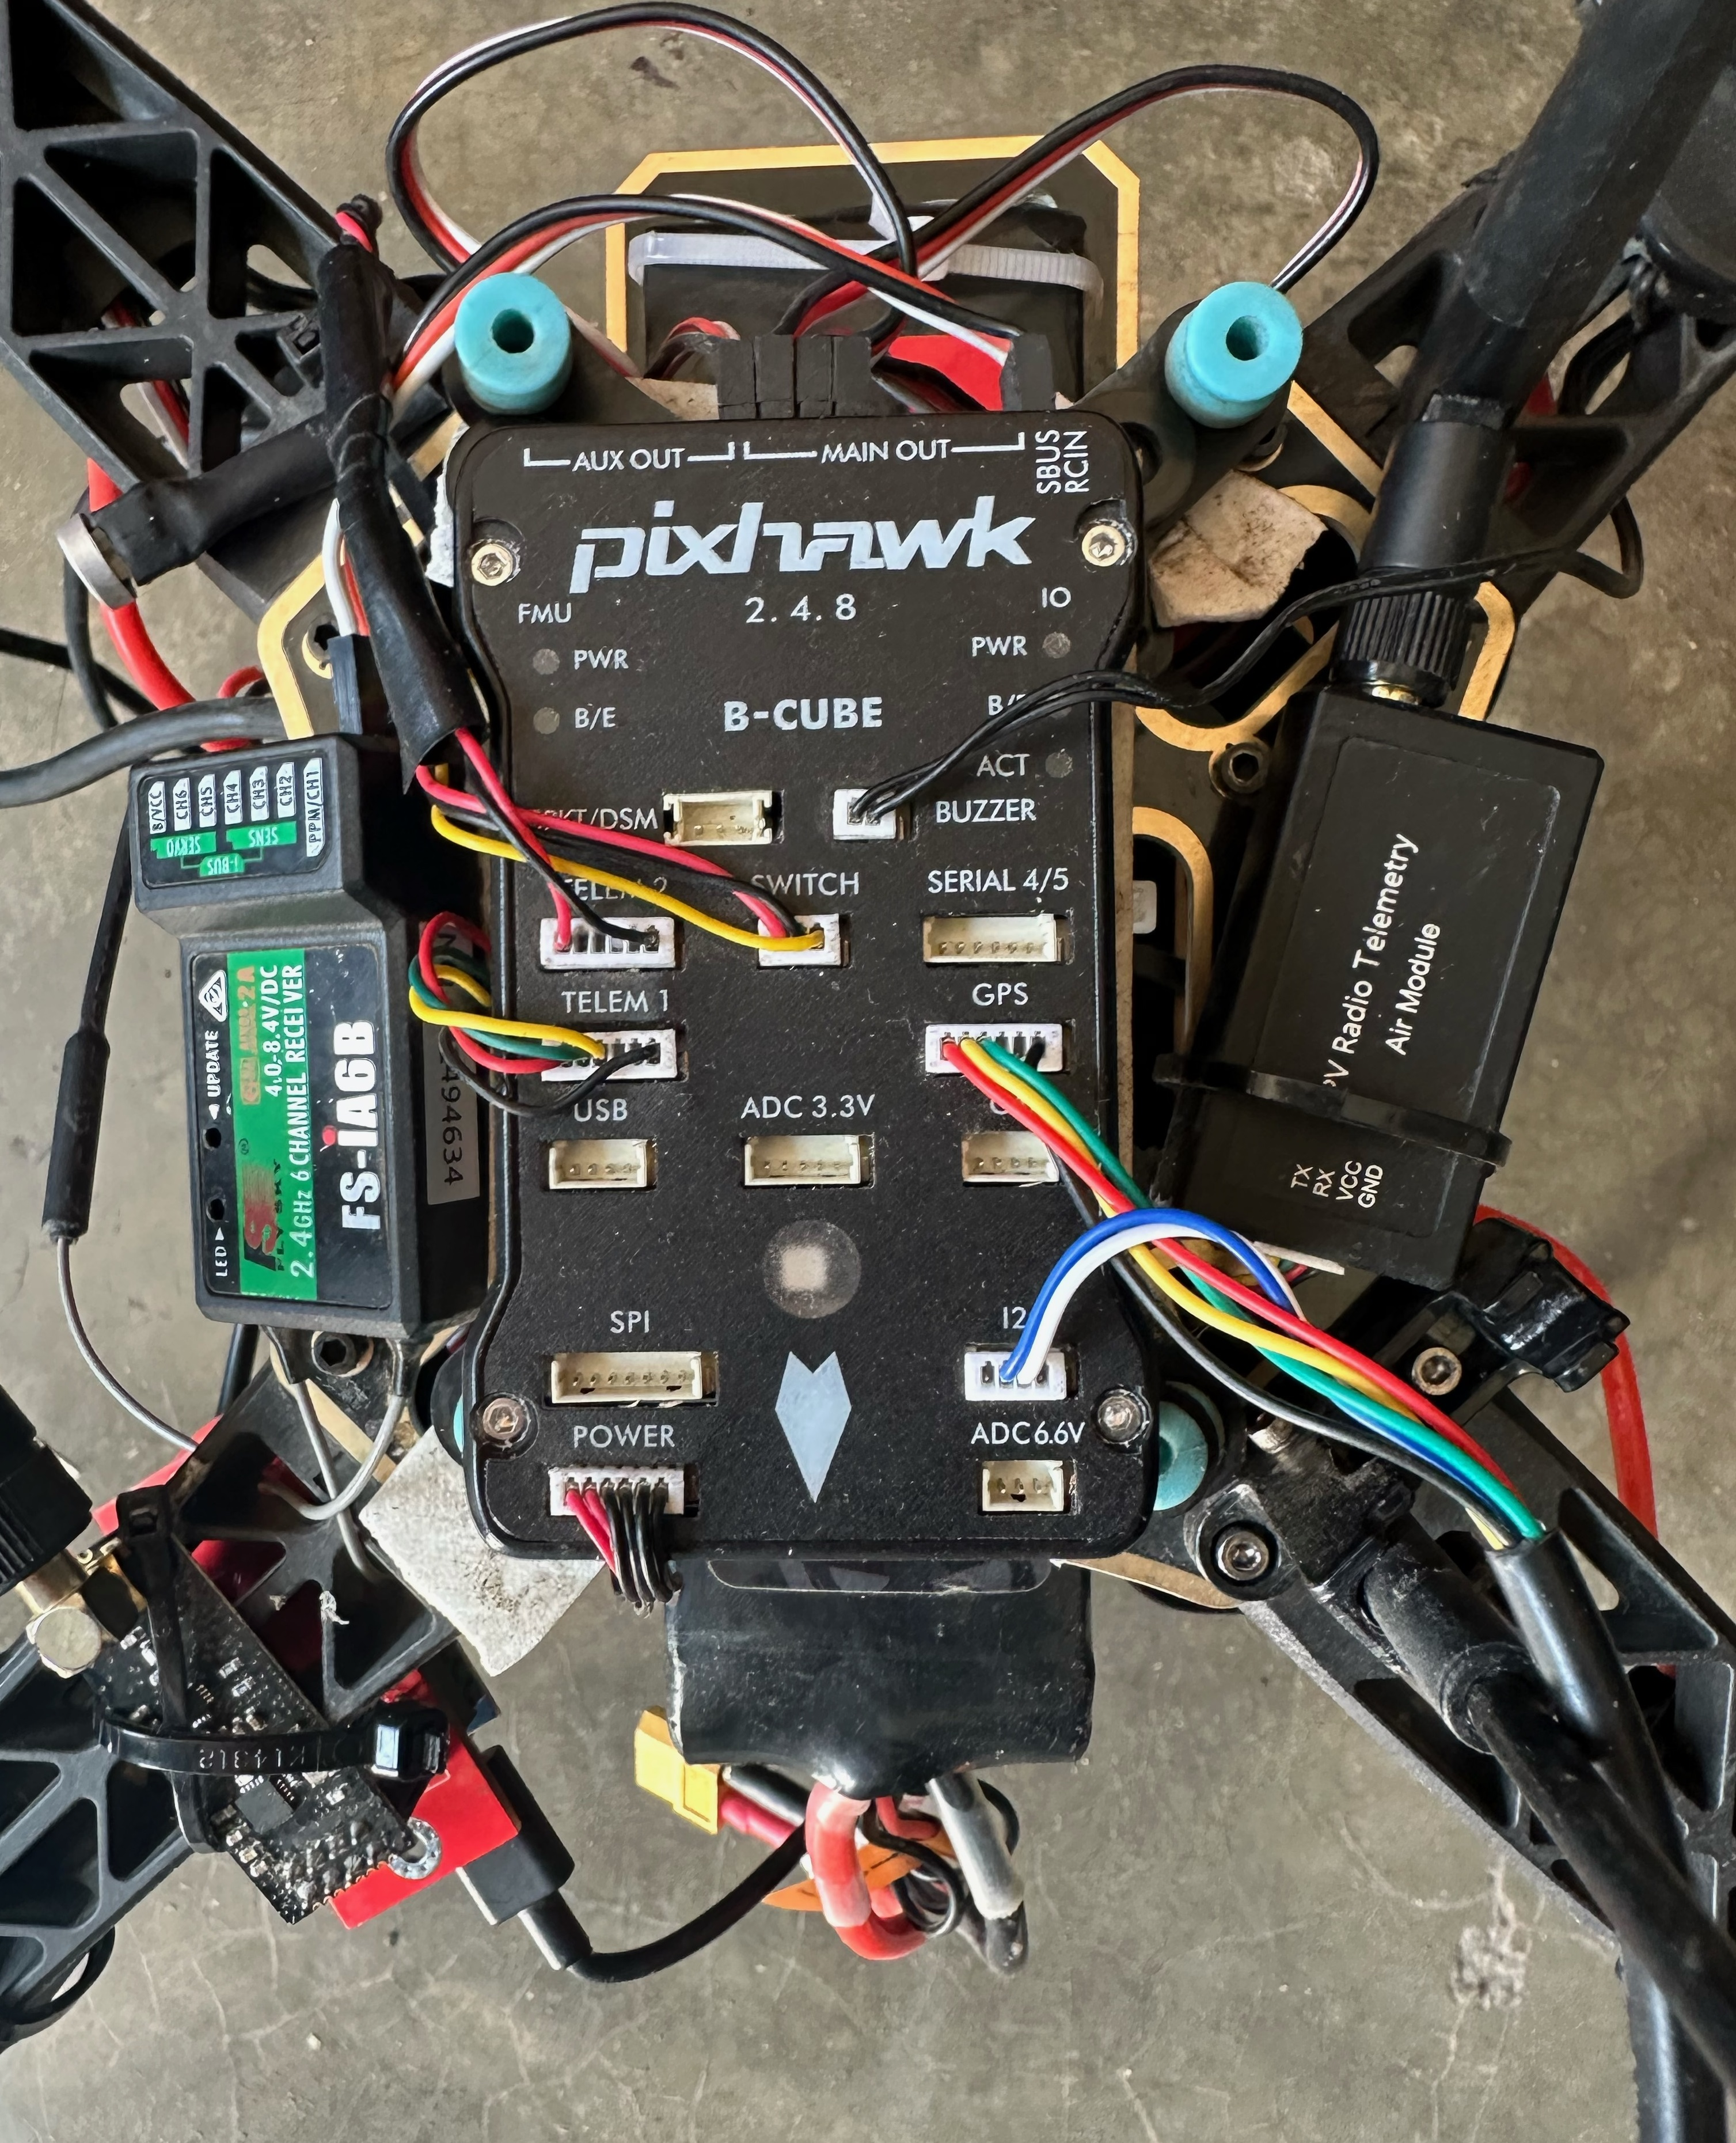
\includegraphics[width=0.5\textwidth, height=7cm]{imagenes/pix.jpeg}
    \caption{Conexiones sobre la computadora de vuelo.}
    \label{fig:basetren}
\end{figure}

\noindent Para la parte específica de control del dron, se le añade otra computadora, la Raspberry Pi4, ya que contiene las librerías para el protocolo MavLink, cuenta con los puertos suficientes para conectar dispositivos y tiene la capacidad de procesar señales digitales (DSP) en caso de ser necesario. Algunos de los usos de la Raspberry Pi 4 para este proyecto podrían incluir:
\begin{itemize}
    \item \textbf{Control de vuelo:} Puede ejecutar algoritmos de control de vuelo y software de navegación para dirigir los drones (enjambre de drones) de manera autónoma o semi-autónoma.
    \item \textbf{Interfaz de usuario y monitoreo:} Se puede utilizar Python para desarrollar una interfaz de usuario en la Raspberry Pi 4 que permita supervisar y controlar los drones de manera intuitiva.
\end{itemize}
Esta computadora externa al ser montada en el dron, se alimenta independientemente de la batería principal utilizando una batería externa.
\begin{figure}[H]
    \begin{minipage}{\textwidth}
        \centering
        \begin{minipage}{\textwidth}
            \centering
            \subfigure[) Individualmente.]{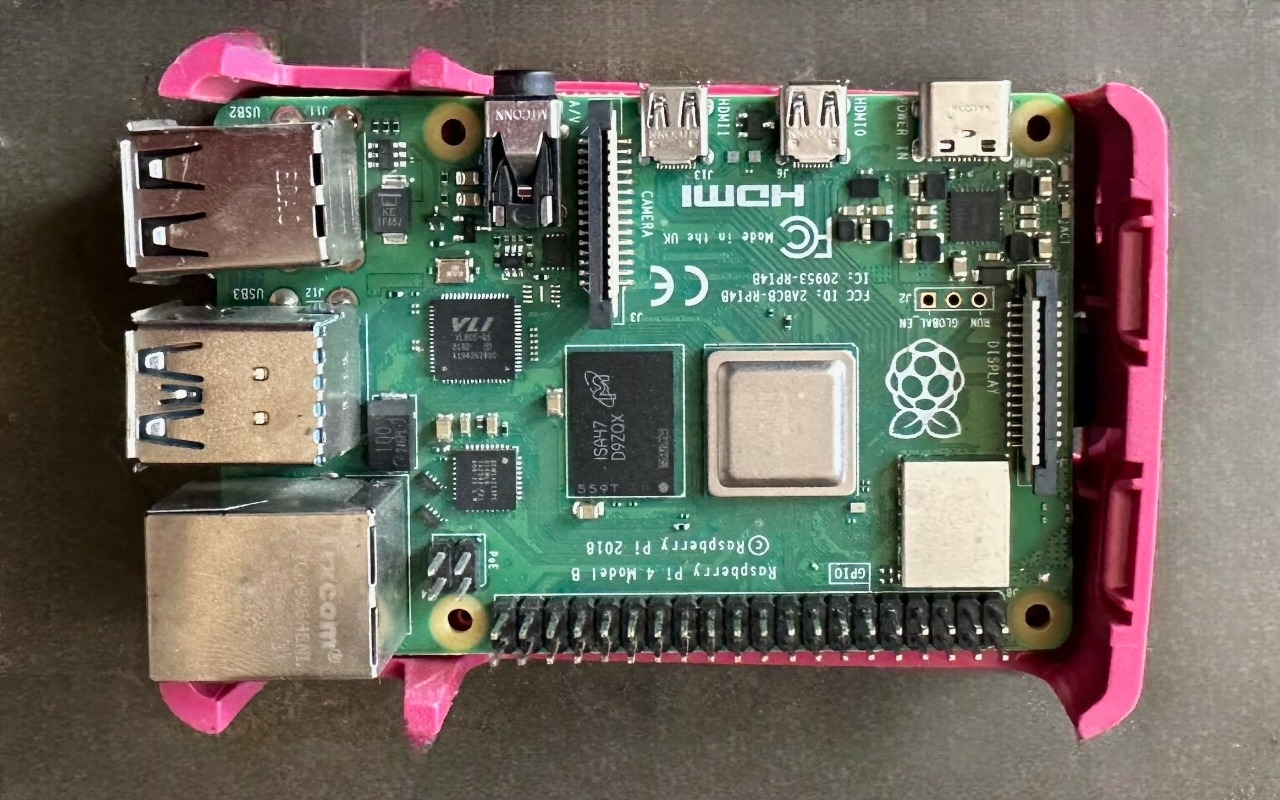
\includegraphics[width=0.45\textwidth, height=4.5cm]{imagenes/rasp.jpeg}}
            \subfigure[) Con batería de 3000mAh.]{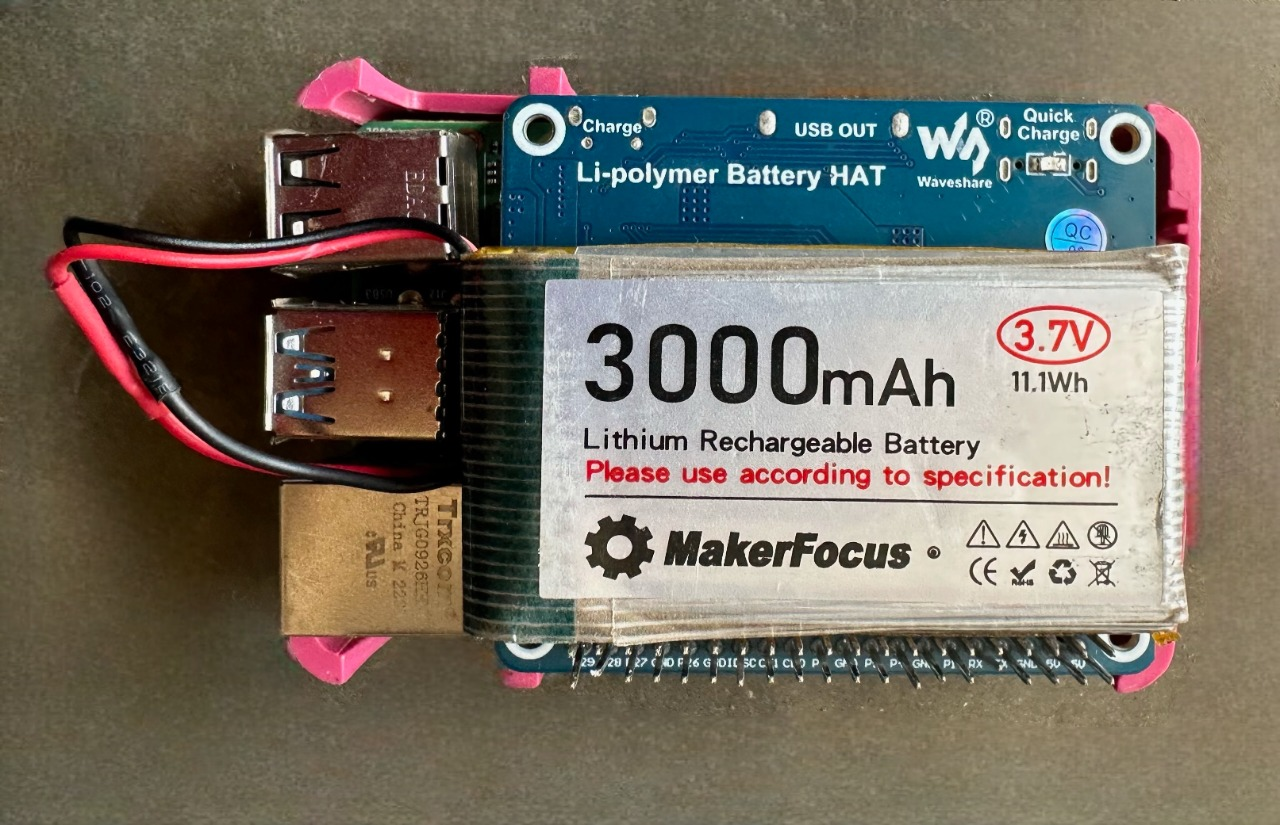
\includegraphics[width=0.45\textwidth, height=4.5cm]{imagenes/rasp-bateria.jpeg}}
        \end{minipage}
    \end{minipage}
    
    \begin{minipage}{\textwidth}
        \centering
        \begin{minipage}{\textwidth}
            \centering
            \subfigure[)  Montada con su batería.]{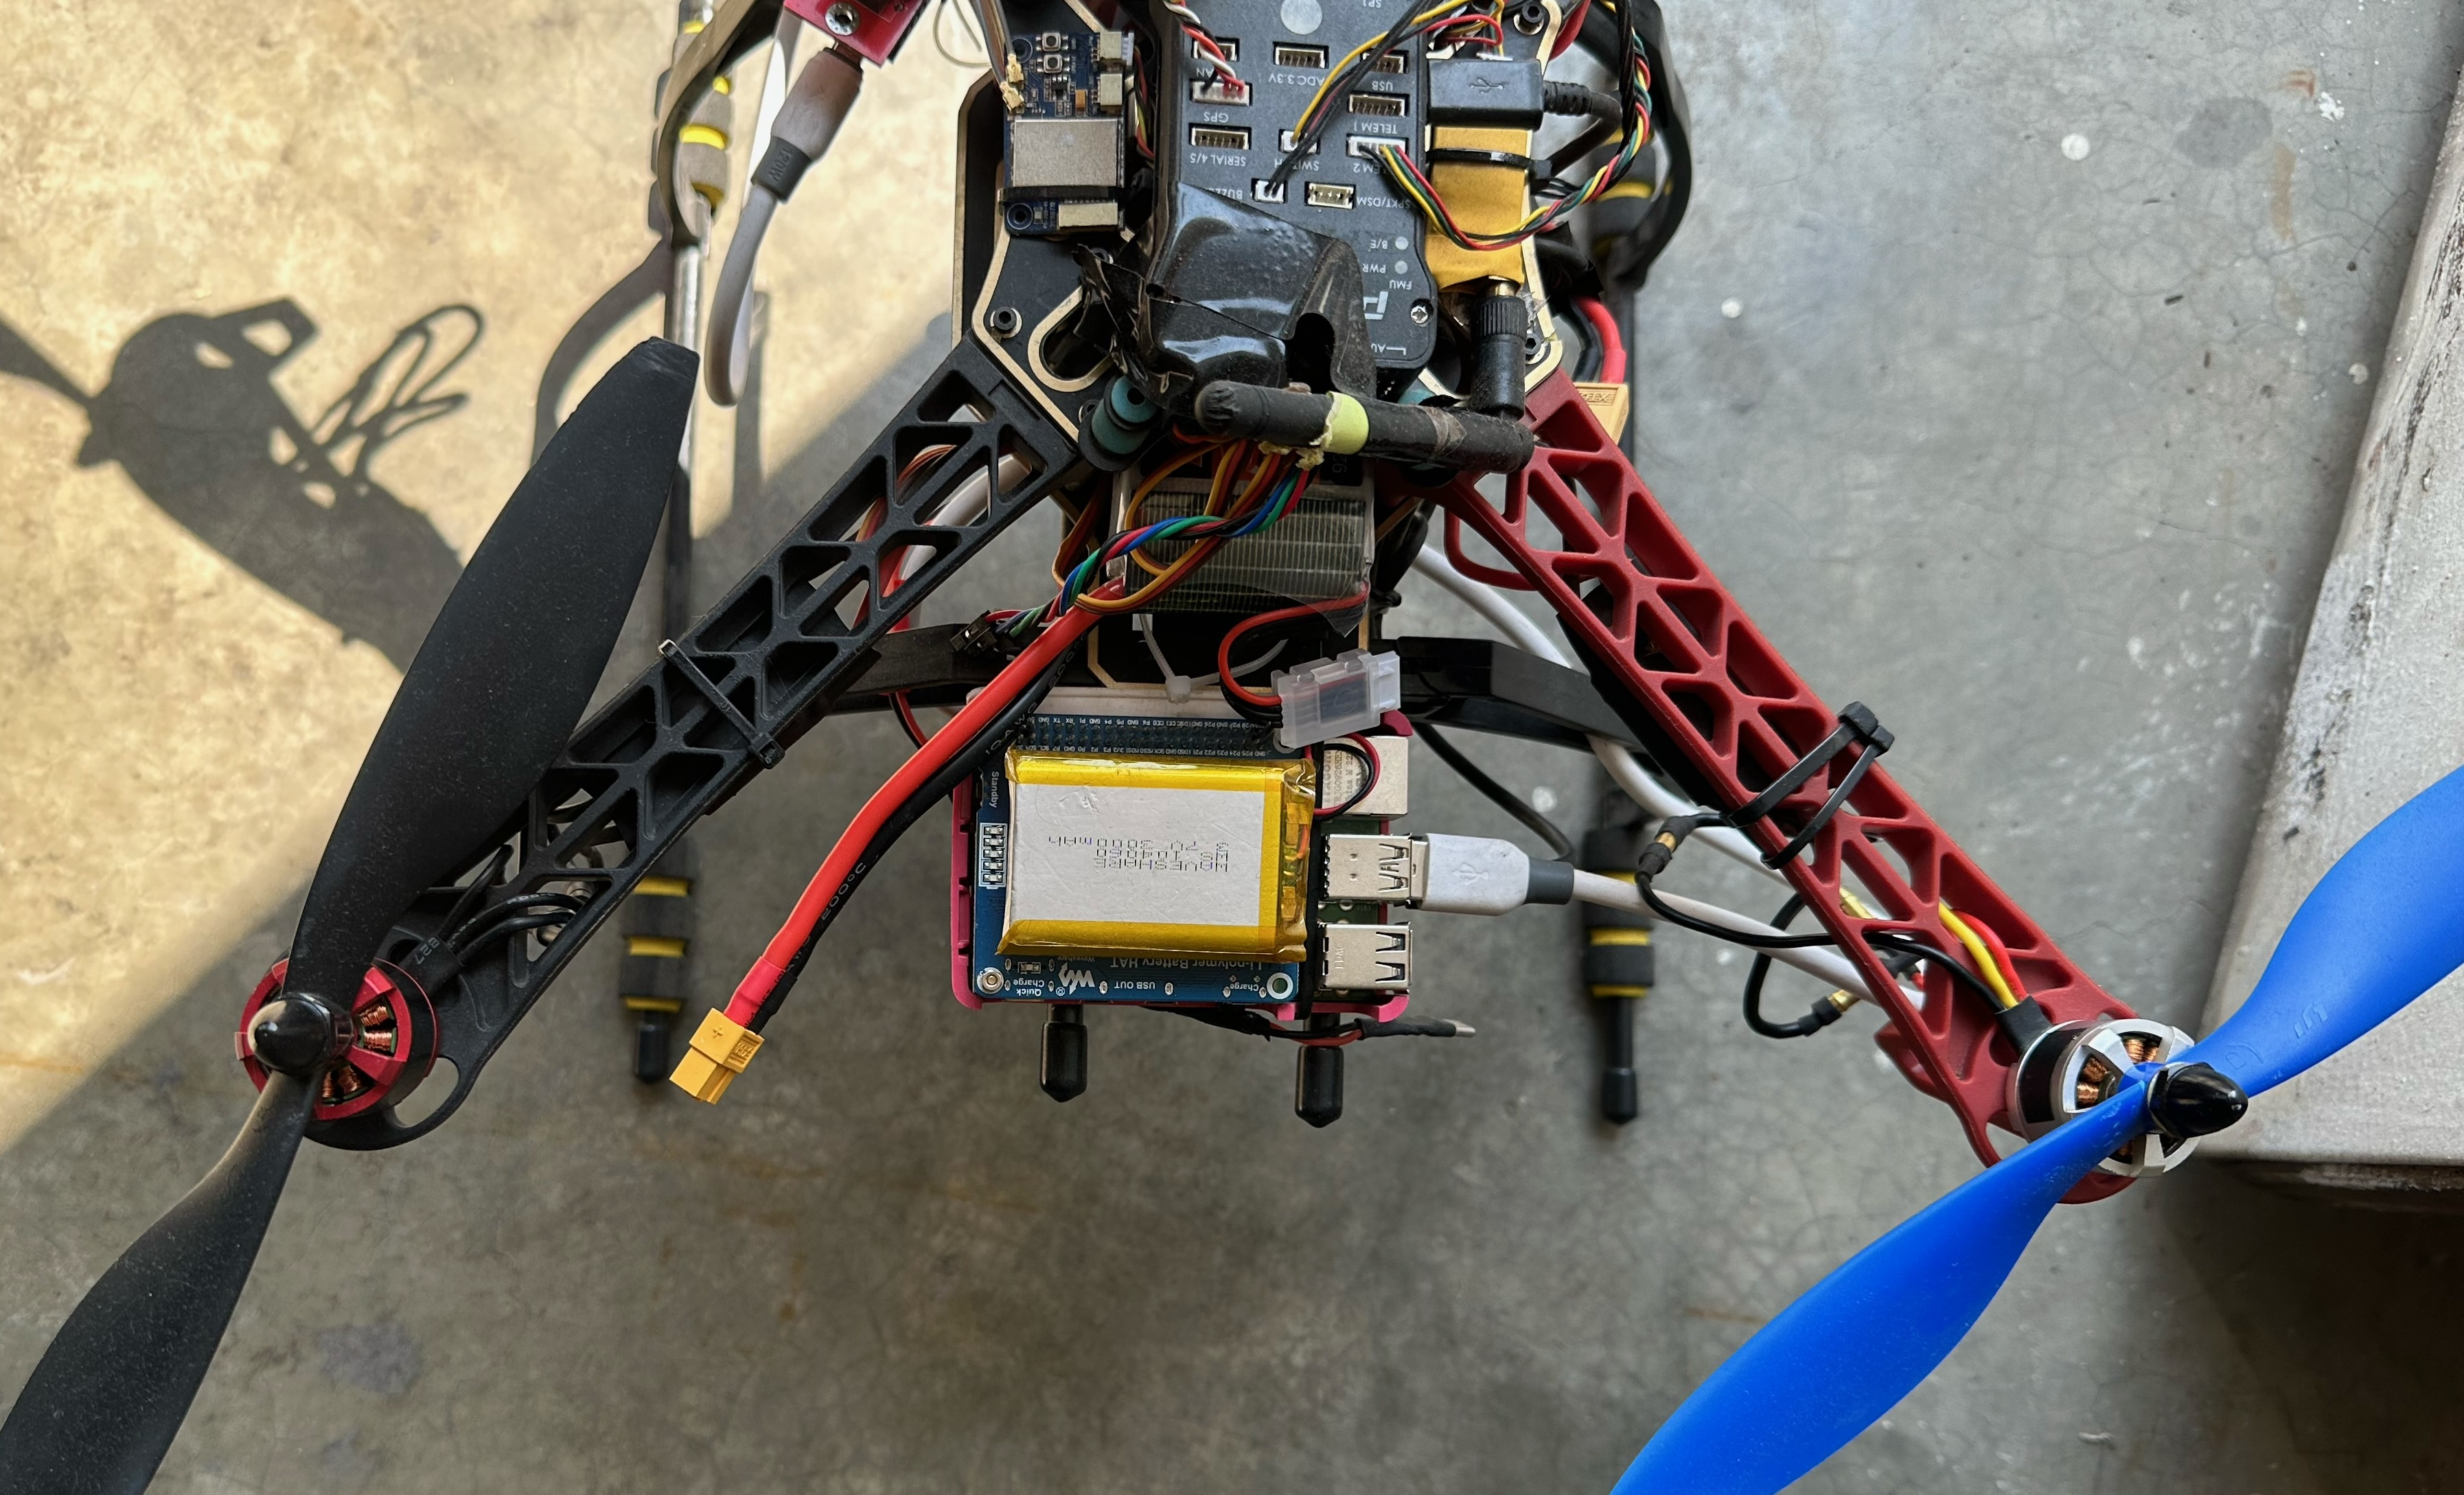
\includegraphics[width=0.45\textwidth]{imagenes/rasp-montada.jpeg}}
        \end{minipage}
    \end{minipage}
    
    \caption{Montaje de la Raspberry Pi4 sobre la placa superior.}
\end{figure}

\noindent Por otra parte, los sistemas de telemetría también son importantes, por lo que para ello se utilizará el módulo NRF24L01. Las características de la telemetría se muestran en la Figura \ref{fig:nrf}:
\noindent Este módulo se puede agregar fácilmente a cualquier sistema MCU/ARM/PIC/AVR/STM32. Además, está diseñado con un amplificador de potencia y antena SMA, lo que le permite utilizar la comunicación inalámbrica hasta a 800 metros (con línea de vista).
\begin{itemize}[itemsep=0pt, parsep=0pt, topsep=0pt, partopsep=0pt]
    \item \textbf{Rango:} 800m de LOS
    \item \textbf{Frecuencia:} 2.4 - 2.5GHz
    \item \textbf{Voltaje de operación:} 3 - 3.6V Max
    \item \textbf{Corriente máxima:} 115mA
\end{itemize}

\noindent Un microcontrolador de anfitrión puede comunicarse y configurar el NRF24L01 a través de una interfaz periférica serial de 4 pines (SPI). Los registros de configuración son accesibles a través de la conexión SPI. Los parámetros configurables incluyen el canal de frecuencia (125 canales seleccionables), la potencia de salida y la velocidad de datos (velocidades de datos: 250kbps, 1Mbps y 2Mbps).

\noindent El regulador de voltaje en el chip acepta voltajes de suministro de 1.9 a 3.6V. El módulo tiene entradas tolerantes a 5V que permiten la conexión directa de los pines SPI.

\noindent El filtrado interno resulta en márgenes altos para cumplir con los estándares regulatorios de RF. La radio del módulo utiliza modulación de desplazamiento de frecuencia gaussiana (GFSK) así como control automático de ganancia rápida (AGC).

\noindent El módulo incluye un pin de solicitud de interrupción (IRQ) que se puede utilizar para despertar al microcontrolador principal del modo de suspensión cuando el módulo recibe una transmisión, lo que proporciona un gran ahorro de energía en dispositivos con batería. 

\begin{figure}[H]
    \centering
    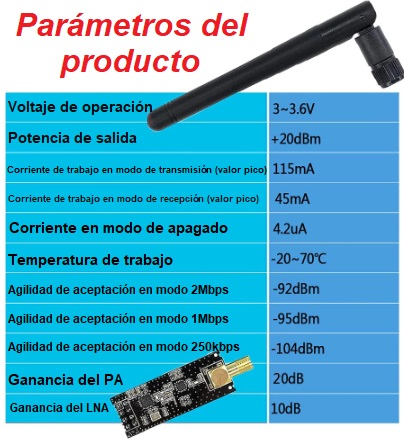
\includegraphics[width=0.6\textwidth, height=7.5cm]{imagenes/parametrosNRF.jpg}
    \caption{Características de la telemetría NRF24L01.}
    \label{fig:nrf}
\end{figure}

\noindent Para cada acción controlable a distancia, se necesita un canal único para transmitir la entrada. El mínimo necesario para pilotar un multirrotor es de cuatro canales: throttle (aceleración), yaw (rotación), pitch (timón) y roll (alerón). Para cada interruptor de modo de vuelo, control de cardán o control de iluminación, se necesita un canal adicional.
\begin{figure}[H]
    \centering
    \includegraphics[width=0.5\textwidth, height=6.5cm]{imagenes/canalización.png}
    \caption{Canalización de Control en Drones Multirrotores.}
    \label{fig:nrf}
\end{figure}

\noindent El Xiangtat Flysky FS-i6X Transmisor con receptor iA6B ayudará a tener un control manual de vuelo para poder controlar el dron desde tierra. El transmisor FS-i6X y el receptor FS-iA6B constituyen un sistema RC computarizado proporcional digital AFHDS 2A de 6 canales. Este sistema ofrece una protección superior contra interferencias mientras mantiene un menor consumo de energía y una alta sensibilidad fiable del receptor. Está especialmente desarrollado para todos los modelos de control de radio. \cite{FLYSKY}

\textbf{Especificaciones del transmisor FS-i6X:}
\begin{itemize}[itemsep=0pt, parsep=0pt, topsep=0pt, partopsep=0pt]
    \item Canales: 6-10 (por defecto 6)
    \item Tipo de modelo: Ala fija/planeador/cuadricóptero
    \item Rango de RF: 2.408 - 2.475 GHz
    \item Potencia RF: < 20dBm
    \item Canal RF: 135
    \item Ancho de banda: 500kHz.
    \item Sistema de 2.4GHz: AFHDS 2A / AFHDS.
    \item Tipo de modulación: GFSK
    \item Resolución del barril: 4096
    \item Advertencia de baja tensión: < 4.2V
    \item Puerto DSC: puerto PS/2
    \item Longitud de la antena: 26mm (antena dual)
    \item Peso: alrededor de 400g
    \item Visualización: visualización transflectiva STN, red LCD de 128 x 64, VA 73 x 39 mm, LCD con retroiluminación blanca
    \item Tamaño: 190 x 174 x 89 mm
    \item Actualización en línea: sí
    \item Certificado: CE0678, FCC ID: N4ZFLYSKYI6X
\end{itemize}
\textbf{Especificaciones del receptor FS-iA6B:}
\begin{itemize}[itemsep=0pt, parsep=0pt, topsep=0pt, partopsep=0pt]
    \item Canales: 6
    \item Rango de RF: 2.4055 - 2.475GHz
    \item Canal RF: 140
    \item Sensibilidad del receptor RF: -105dBm
    \item Ancho de banda: 500kHz
    \item Sistema de 2.4GHz: AFHDS 2A
    \item Tipo de modulación: GFSK
    \item Potencia: 4.0 - 6.5V
    \item Transmisor compatible: FS-i6X, FS-i4, FS-i6, FS-i10, FS-GT2E, FS-GT2G
    \item Longitud de la antena: 26mm (antena dual)
    \item Peso: 16.3g
    \item Tamaño: 47 x 26.2 x 15 mm
    \item Puerto i-bus: sí
    \item Puerto de adquisición de datos: sí
\end{itemize}

\begin{figure}[H]
    \centering
    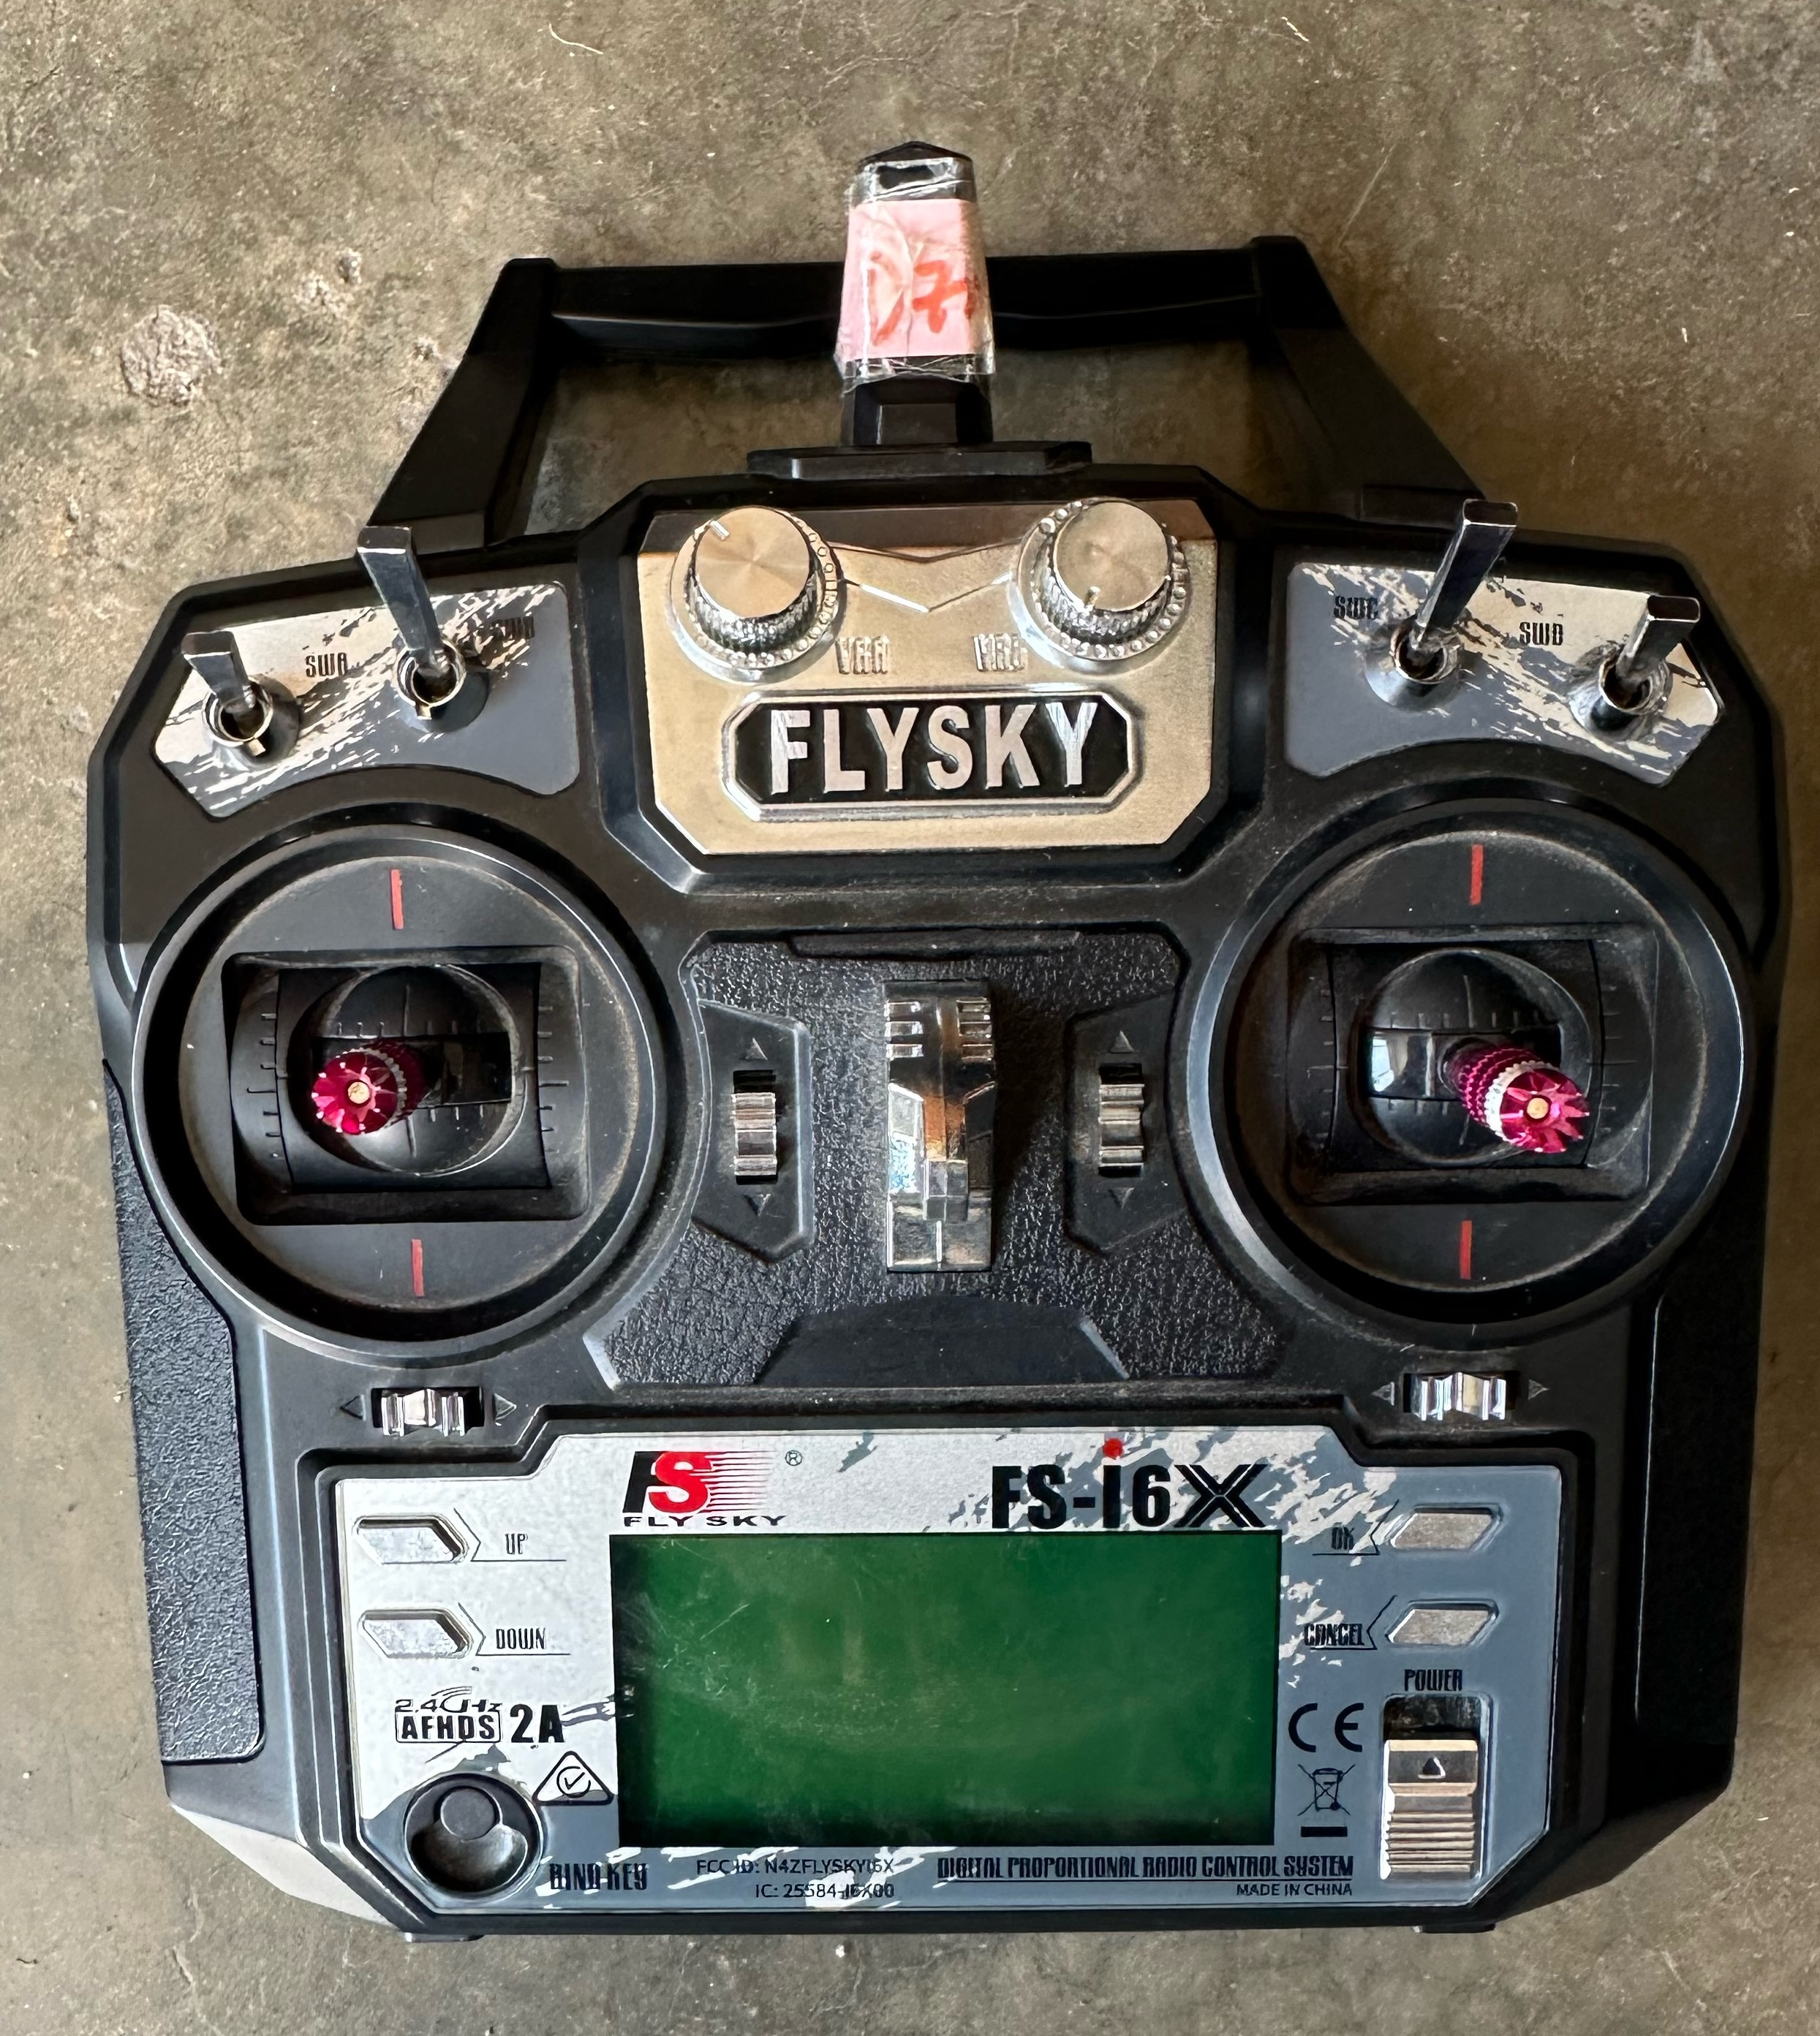
\includegraphics[width=0.45\textwidth]{imagenes/control.jpeg}
    \caption{Transmisor Radio Controlado.}
    \label{fig:control}
\end{figure}

\noindent En cuanto a la batería del dron, esta se coloca ajustadamente entre la placa inferior y la placa superior para evitar su deslizamiento. Tomando en cuenta que para no reducir su tiempo de vida, no se debe permitir que sus celdas se descarguen menos del 80\% (para una batería de 12V no se debe descargar a menos de 9.6V). Su capacidad y corriente por hora dependen del consumo energético del UAV:
\begin{itemize}
    \item Entre más grande más consumo
    \item Entre más propelas más consumo
    \item Entre más dispositivos conectados, más consumo
    \item Entre más velocidad y movimiento, más consumo
\end{itemize}

\begin{table}[H]
    \centering
    \caption{Relación de la capacidad de la batería con el tamaño de las hélices.}
    \begin{tabular}{|c|c|}
        \hline
        \cellcolor[HTML]{C0C0C0}Tamaño de las hélices & \cellcolor[HTML]{C0C0C0}Capacidad de la batería \\
        \hline
        6” & 1500 mAh a 2200 mAh \\
        \hline
        5” & 1300 mAh a 1800 mAh \\
        \hline
        4” & 850 mAh a 1300 mAh \\
        \hline
        3” & 650 mAh a 1000 mAh \\
        \hline
    \end{tabular}
    \label{tab:battery_helices}
\end{table}

\noindent El tiempo de vuelo está relacionado al consumo energético de la batería y se puede calcular a partir de la corriente que consume el dron, la batería, el peso, la mínima descarga del dron, etc. Existen modelos matemáticos (e.g. Backstepping) y simuladores (e.g. ROS Gazebo) que pueden predecir el consumo energético de un UAV \cite{videodron}.

\begin{figure}[H]
    \centering
    \subfigure[) Individualmente.]{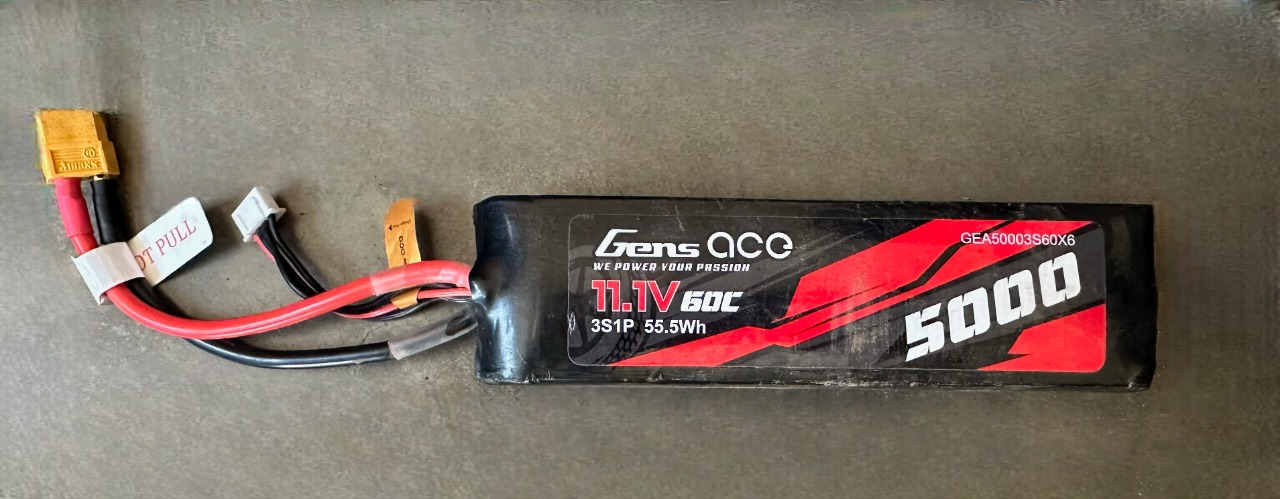
\includegraphics[width=0.45\textwidth, height=4cm]{imagenes/bateria.jpeg}}
    \quad
    \subfigure[) Montada.]{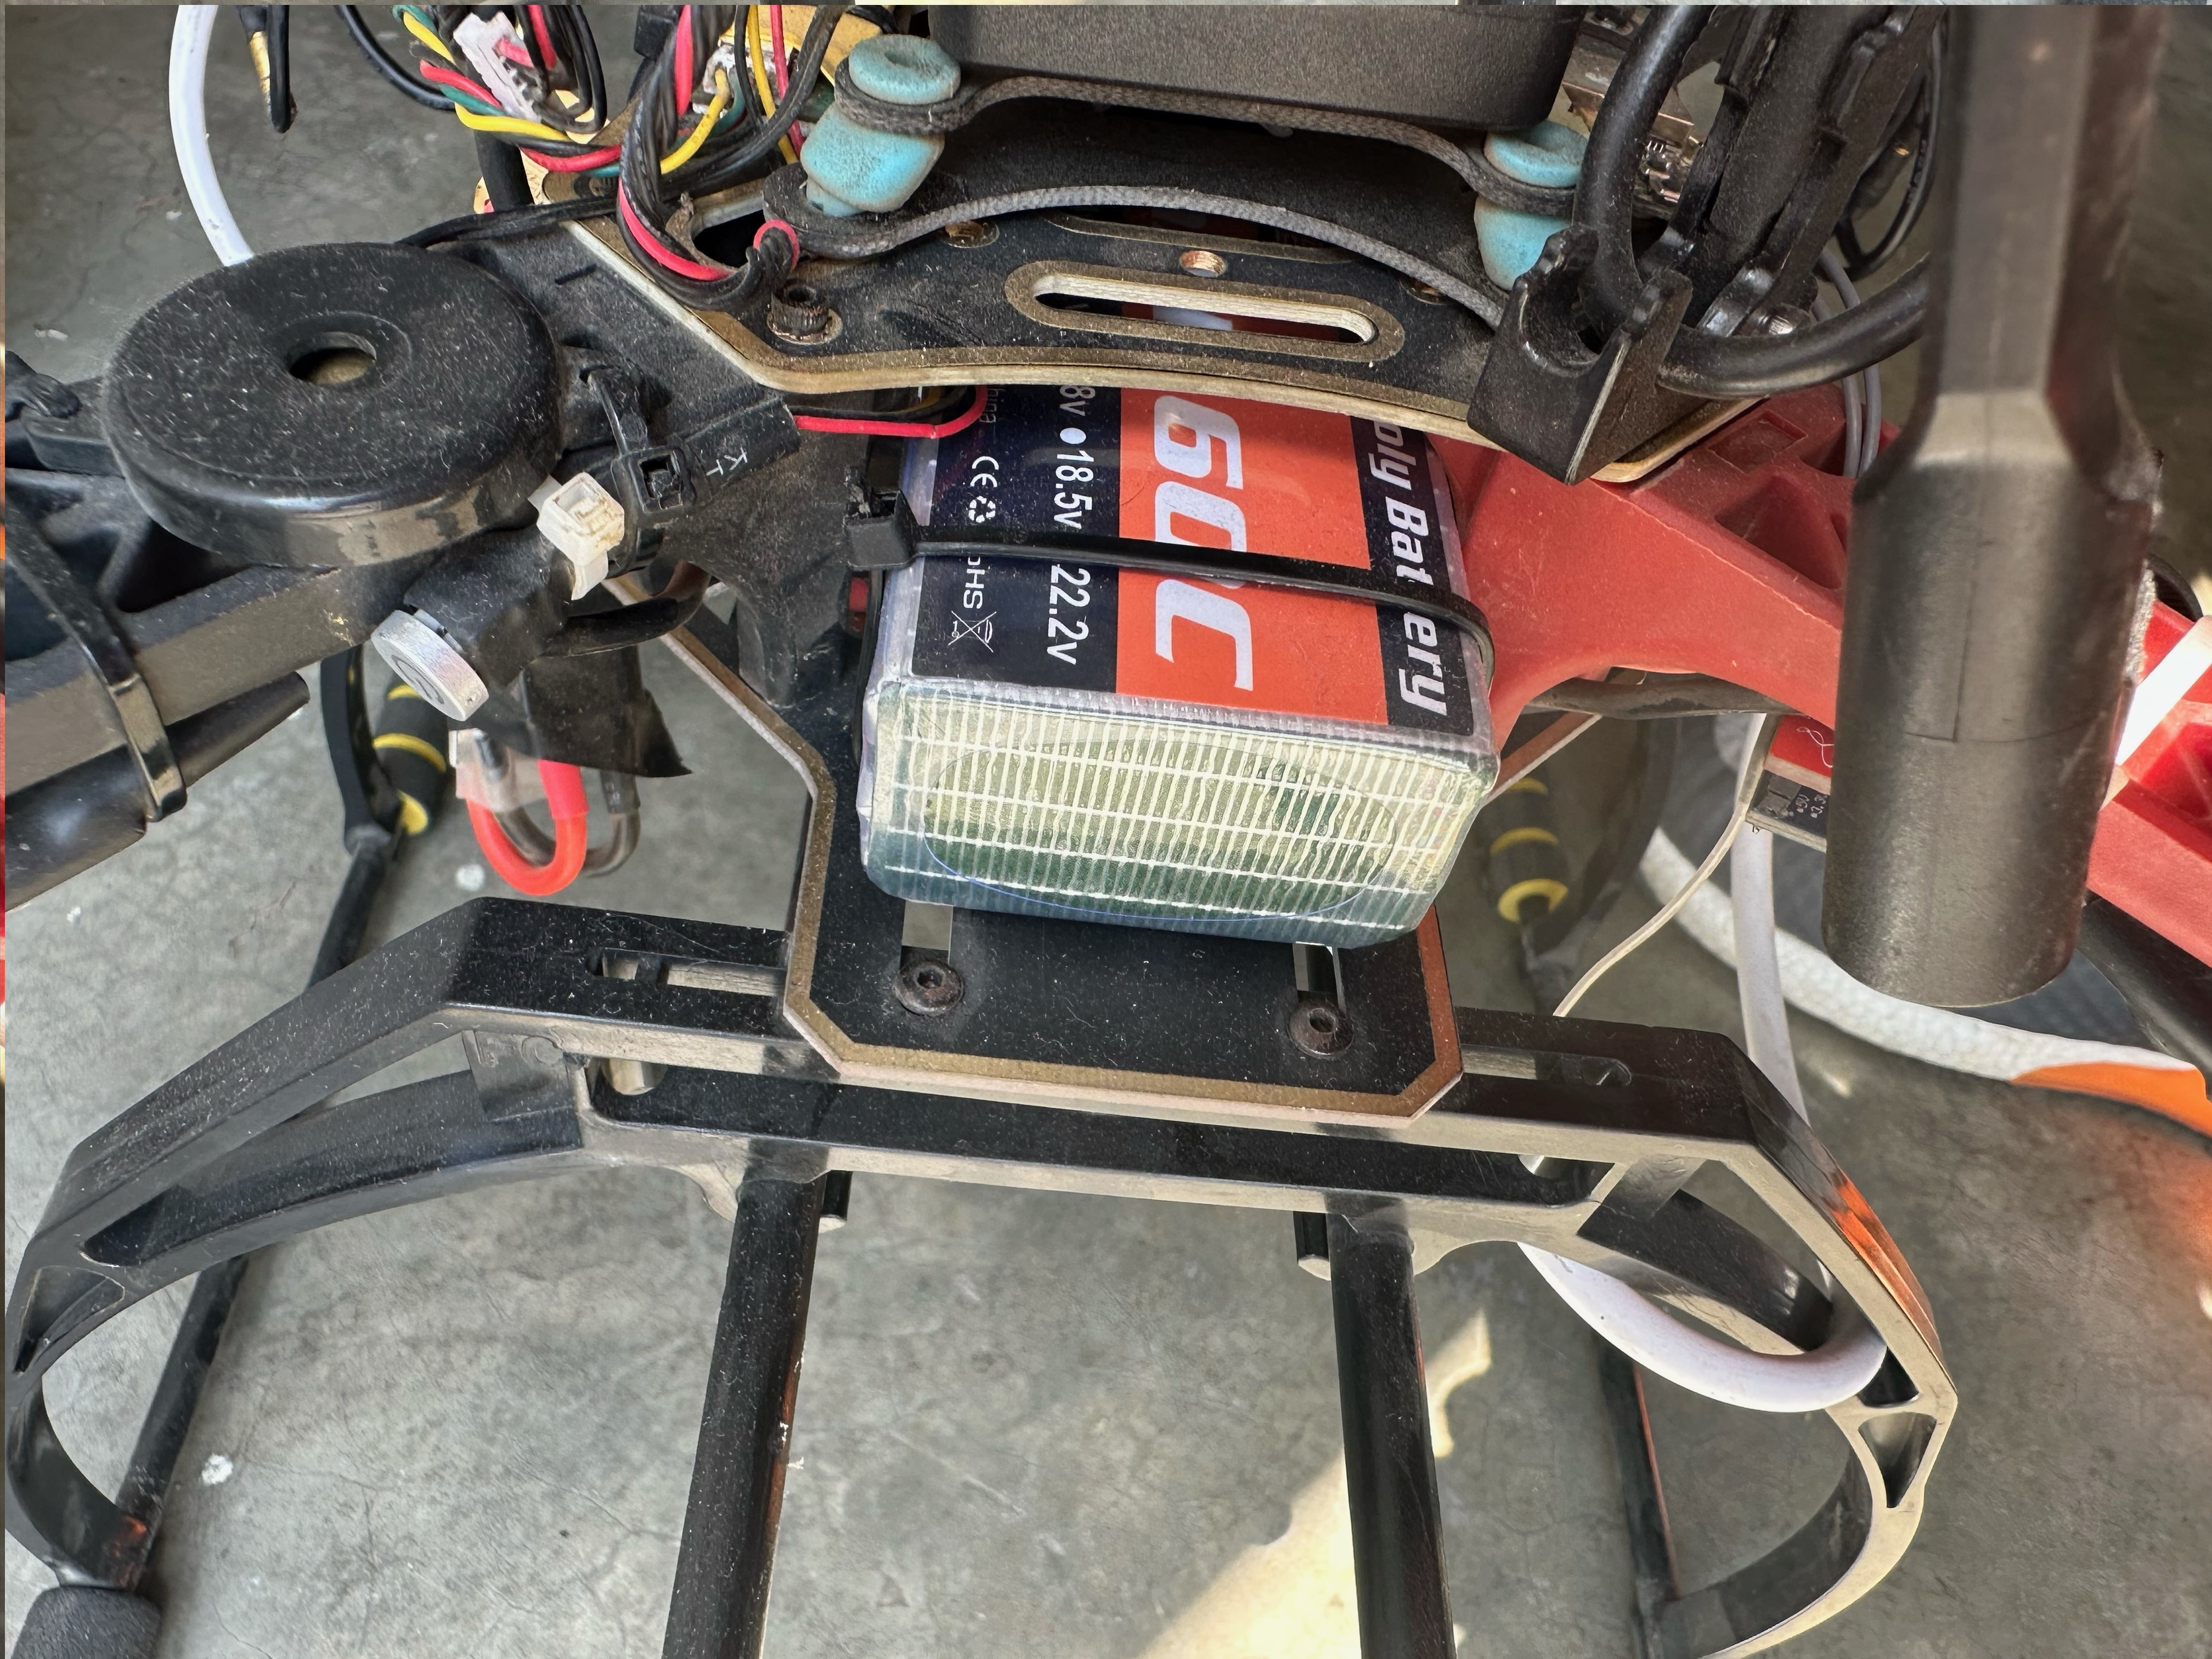
\includegraphics[width=0.45\textwidth, height=4cm]{imagenes/bateria-montada.jpeg}}
    \caption{Montaje de la batería 5000mAh 6 celdas 22.2v 25C-60C RC sobre la placa inferior.}
    \label{fig:bateria}
\end{figure}


\noindent Ya por último, podemos ver en la Figura \ref{fig:drone} el dron completamente armado con todos los componentes ensamblados y montados sobre la estructura y las placas del dron.

\begin{figure}[H]
    \centering
%    \includegraphics[width=0.5\textwidth]{imagenes/}
    \caption{Dron listo para pruebas de vuelo.}
    \label{fig:drone}
\end{figure}

\noindent Estos mismos procesos se hacen para el ensamblado de los otros dos prototipos, más adelante se seguirán haciendo pruebas y documentación sobre las demás actividades para modelar el consumo energético y los esquemas de vuelo para la recolección de datos.
\begin{figure}[H]
    \centering
    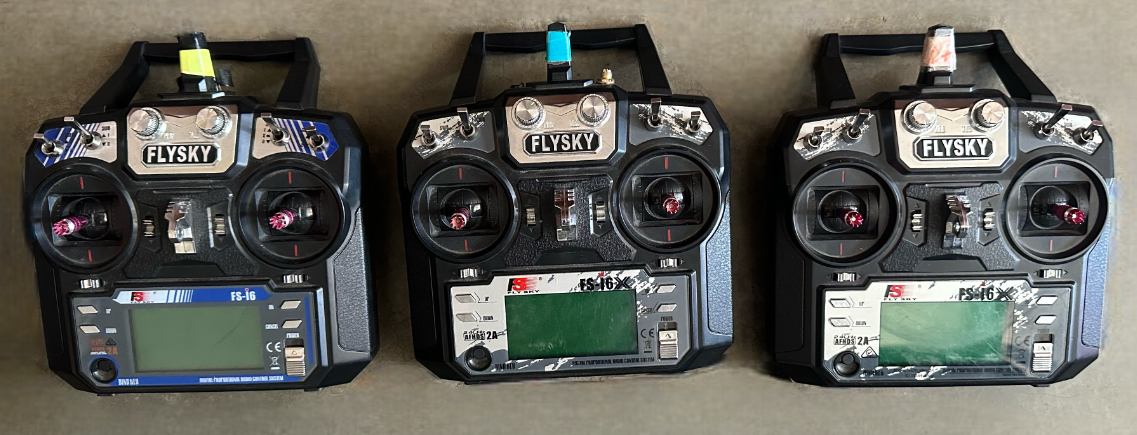
\includegraphics[width=0.85\textwidth]{imagenes/controles.png}
    \caption{Transmisores de Radio Control para cada dron .}
    \label{fig:drones}
\end{figure}
\begin{figure}[H]
    \centering
    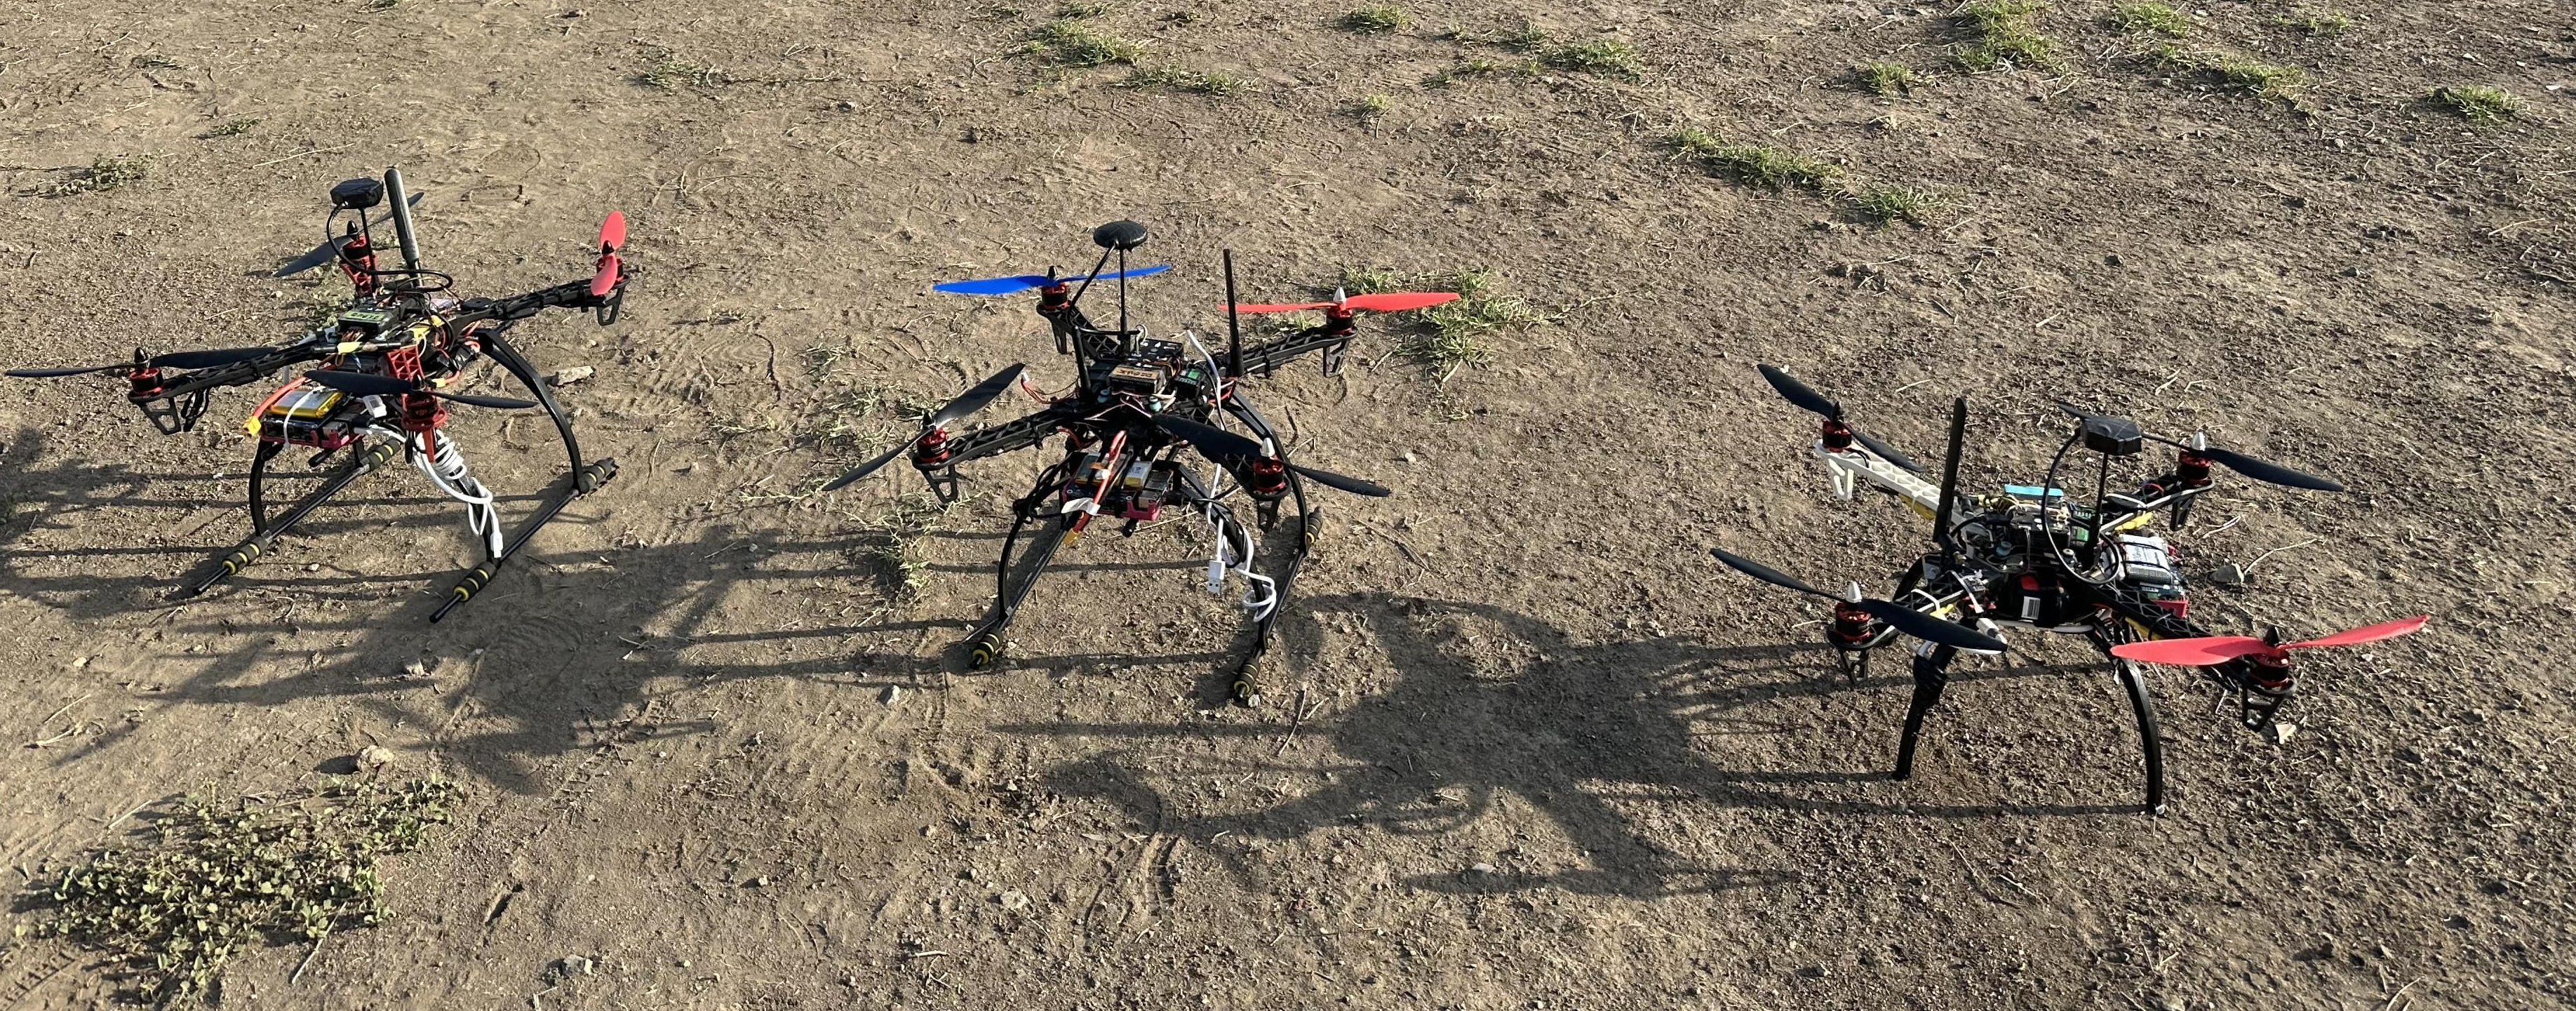
\includegraphics[width=0.85\textwidth, height=6cm]{imagenes/tres-drones.jpg}
    \caption{Drones listos para pruebas de vuelo.}
    \label{fig:drones}
\end{figure}

\noindent Por último, se describe el proceso de vuelo coordinado del enjambre de drones en el diagrama de flujo de la Figura \ref{fig:diagrama-vuelo-enjambre}. Comenzando con la inicialización de los dispositivos involucrados, donde, se encienden los tres drones, que consisten en el dron líder y los dos drones seguidores. Simultáneamente, la estación base se conecta a un monitor serial, lo que permite la comunicación con el dron líder desde la estación base.

\noindent Una vez encendidos los drones, cada uno de ellos obtiene sus coordenadas GPS. Los drones seguidores envían sus coordenadas al dron líder, quien recopila y envía estas coordenadas junto con las propias a la estación base. Este ciclo de envío de coordenadas se repite continuamente hasta estas que todas se reciban en la estación base y se muestren en el monitor serial.

\noindent La estación base verifica entonces si ha recibido todas las coordenadas necesarias. No se puede continuar el proceso si no se han recibido las coordenadas de todos los drones en la estación base. 

\noindent Una vez que la estación base ha recibido todas las coordenadas, se envía un comando de inicio al dron líder. Este comando indica al dron líder que debe prepararse para iniciar el vuelo coordinado. Si el comando ha sido recibido correctamente, el dron líder envía un comando de despegue a los drones seguidores para que todos los drones despeguen simultáneamente.

\noindent Una vez en vuelo, cada dron sigue su ruta programada. Este seguimiento de ruta se mantiene mientras el vuelo esté en progreso, asegurando que los drones se desplacen de acuerdo con sus planes de vuelo configurados. Finalmente, el proceso concluye cuando los drones regresan a la estación base, finalizando el procedimiento de vuelo en enjambre o coordinado.

\begin{figure}[H]
    \centering
    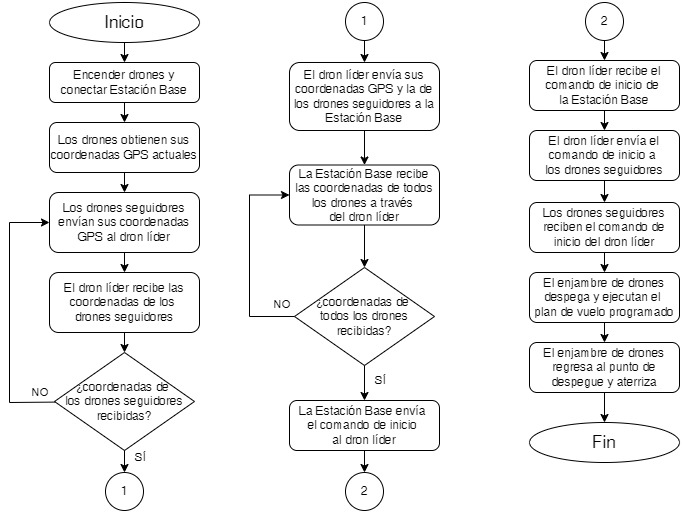
\includegraphics[width=0.95\textwidth]{imagenes/diagrama-enjambre.jpg}
    \caption{Diagrama de flujo para el vuelo en enjambre.}
    \label{fig:diagrama-vuelo-enjambre}
\end{figure}


\subsection{Configuración de los Drones.}
Para configurar los drones se hacen una serie de pasos para calibrar y corroborar que los componentes funcionen. Para comenzar, conectaremos nuestra computadora de vuelo directamente a nuestra computadora o por telemetría.

\begin{figure}[H]
	\centering
	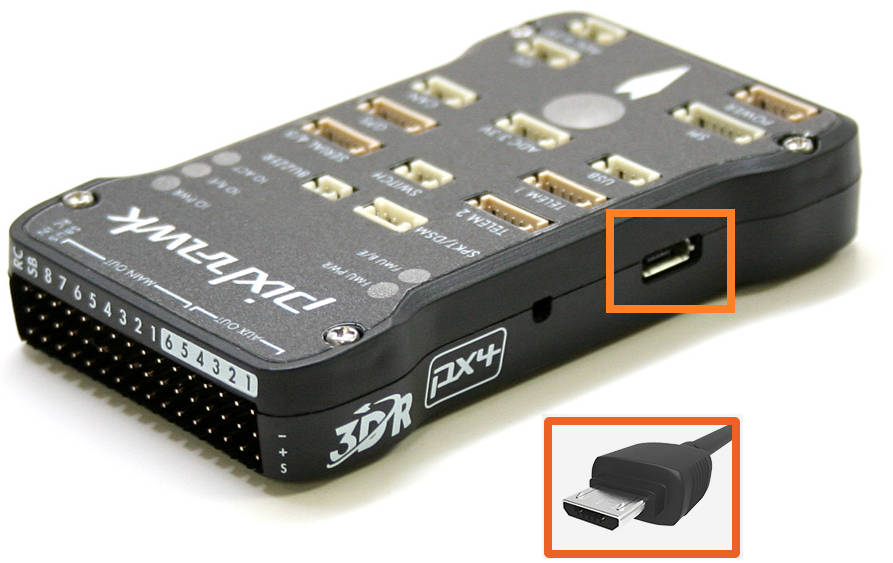
\includegraphics[width=0.7\linewidth]{imagenes/pixhawk}
	\caption{Conexión de la Computadora devuelvo a la computadora por cable.}
	\label{fig:pixhawk}
\end{figure}

\subsubsection{Calibración de la brújula. (Compass Calibration)}

Dentro de las configuraciones más importantes y que siempre hacemos antes de empezar un vuelo, calibramos la brújula. Una vez conectada nuestra telemetría a nuestra computadora, abriremos el software “Mission Planner” para configurar la brújula siguiendo los siguientes pasos:

 En la pestaña \textit{Setup} \textrightarrow \textit{Mandatory Hardware} \textrightarrow \textit{Compass}, nos aparecerá la siguiente ventana.

\begin{figure}[H]
	\centering
	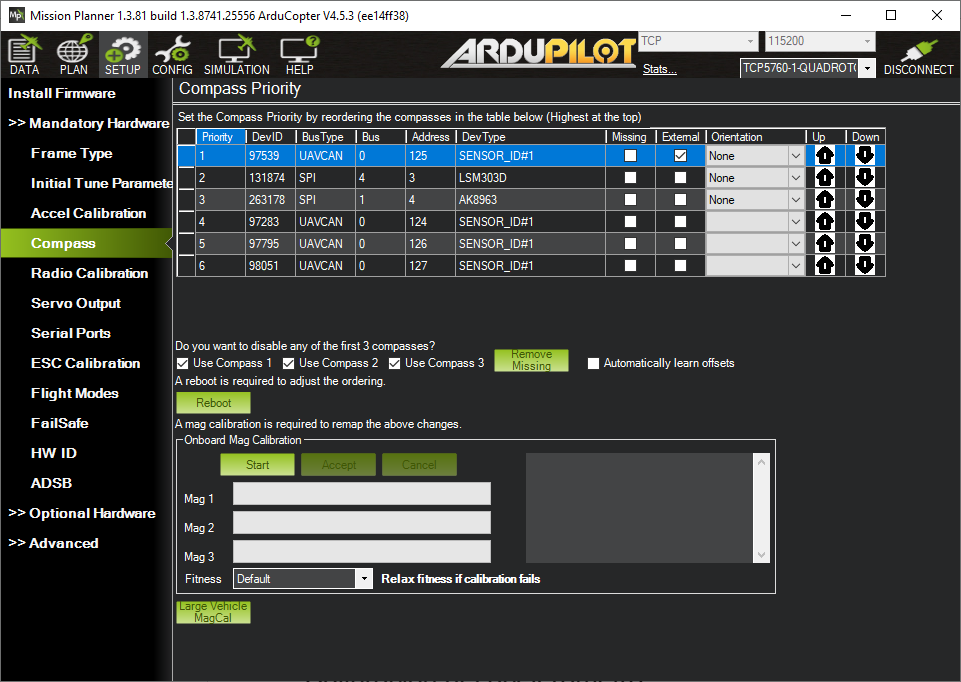
\includegraphics[width=\linewidth]{imagenes/compass}
	\caption{Calibración de la brújula}
	\label{fig:compass}
\end{figure}

Observaremos que contamos con barrios GPS en nuestra ventana, es importante tener en cuenta que le debemos dar prioridad a nuestro GPS externo que lo marcaremos con la casilla de “External”, nuestra computadora de vuelo también incluye un GPS, así que ese dispositivo también sa calibrará con estos pasos.
Como nota, el Dron debe no estar armado y no se debe calibrar cerca de algún dispositivo electrónico ni metálico, ya que puede afectar la forma de calibración del GPS.

Continuando con la calibración, al dar click en el botón Start dentro de la sección de “On board Mag Calibration” y se debe mover el Dron en los 360°, dando vueltas, moviéndolo de izquierda a derecha, poniéndolo de cabeza y en todas las direcciones posibles.
A medida que se gira el vehículo, las barras verdes deben extenderse cada vez más hacia la derecha hasta que se complete la calibración.
Una vez finalizado con éxito, se emitirán tres tonos ascendentes y aparecerá una ventana de "Reinicie el piloto automático" y deberá reiniciar el auto Pilot antes de que sea posible armar el vehículo


\subsubsection{Calibración del acelerómetro (Accel Calibration).}

Los acelerómetros del Dron deben calibrarse para corregir sus desplazamientos de polarización en los tres ejes (Pitch, Yaw y Roll). La calibración del acelerómetro es obligatoria en ArduPilot y la calibración no se puede realizar mientras el vehículo está armado.
Nos dirigimos a la calibración del acelerómetro siguiendo las siguientes rutas:

En la pestaña \textit{Setup} \textrightarrow \textit{Mandatory Hardware}\textrightarrow \textit{Accel Calibration}, nos aparecerá la siguiente ventana.

\begin{figure}[H]
	\centering
	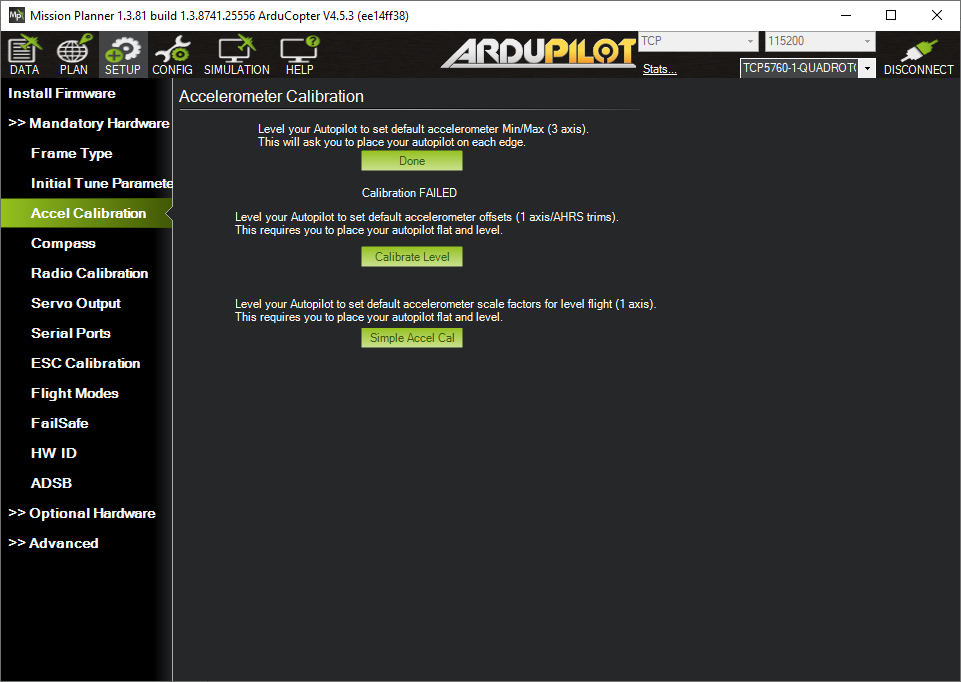
\includegraphics[width=0.9\linewidth]{imagenes/accel}
	\caption{Ventana de Calibración del acelerómetro.}
	\label{fig:accel}
\end{figure}
\newpage
Deberemos hacer click en la primera opción, seguido de eso, el propio software, nos indicará las posiciones en las que debemos colocar el Dron, las posiciones son:

\begin{itemize}
	\item Level. \textit{(En el nivel del suelo)}.
	\begin{figure}[H]
		\centering
		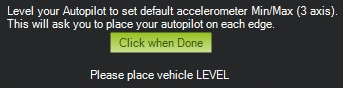
\includegraphics[width=0.6\linewidth]{imagenes/conf1}
		\caption{}
		\label{fig:conf1}
	\end{figure}
	
	\item Left. \textit{(Izquierda)}.
	\begin{figure}[H]
		\centering
		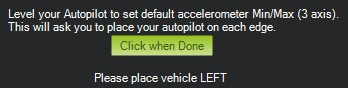
\includegraphics[width=0.6\linewidth]{imagenes/conf2}
		\caption{}
		\label{fig:conf1}
	\end{figure}
	
	\item Right. \textit{(Derecha).}
	\begin{figure}[H]
		\centering
		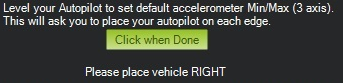
\includegraphics[width=0.6\linewidth]{imagenes/conf3}
		\caption{}
		\label{fig:conf1}
	\end{figure}
	
	\item Nose Down. \textit{(Con la parte frontal del Dron mirando hacia abajo).}
	\begin{figure}[H]
		\centering
		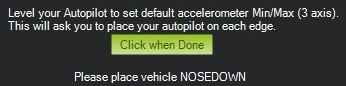
\includegraphics[width=0.6\linewidth]{imagenes/conf4}
		\caption{}
		\label{fig:conf1}
	\end{figure}
	
	\item Nose Up.\textit{ (Con la parte frontal del Dron mirando hacia arria).}
	\begin{figure}[H]
		\centering
		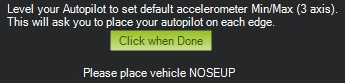
\includegraphics[width=0.6\linewidth]{imagenes/conf5}
		\caption{}
		\label{fig:conf1}
	\end{figure}
	
	\item Back. \textit{(Con la parte superior del Dron mirando hacia abajo).}
	\begin{figure}[H]
		\centering
		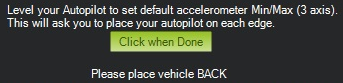
\includegraphics[width=0.6\linewidth]{imagenes/conf6}
		\caption{}
		\label{fig:conf1}
	\end{figure}
	
	
\end{itemize}

El Dron debe mantenerse quieto inmediatamente después de presionar la tecla para cada posición. Esto es más importante que conseguir el ángulo exacto, es decir  a la izquierda a 90 grados a horizontal exactamente, etc. A excepción del primer "NIVEL", las posiciones pueden estar dentro de los 20 grados (por inclinación del suelo) de ser exactas. Se debe estar quieto en cada posición mientras presionamos la tecla de aceptar.
La posición de nivel es la más importante de todas para la calibración, ya que esta será la posición que el Dron considere nivelada mientras vuela.

\subsubsection{Configuración del Control.}

Los controles transmisores nos permiten configurar el modo de vuelo, controlar el movimiento y la orientación del vehículo y también activar y desactivar las funciones auxiliares (es decir, subir y bajar el tren de aterrizaje, etc.) de las cuales hablaremos más adelante.

La calibración del control implica la captura de los valores mínimos, máximos y de "ajuste" de cada canal para que ArduPilot pueda interpretar correctamente la entrada.

Antes de comenzar, hay que asegurarnos de que el control tenga una batería con carga, al momento de encender el control verificar que esté en “Auto” y que las lengüetas del control se encuentren totalmente levantadas..

Para abrir el menú de configuración, nos dirigiremos a:
\textit{Setup} \textrightarrow \textit{ Mandatory Hardware} \textrightarrow \textit{Radio Calibration}, nos aparecerá la siguiente ventana.

\begin{figure}[H]
	\centering
	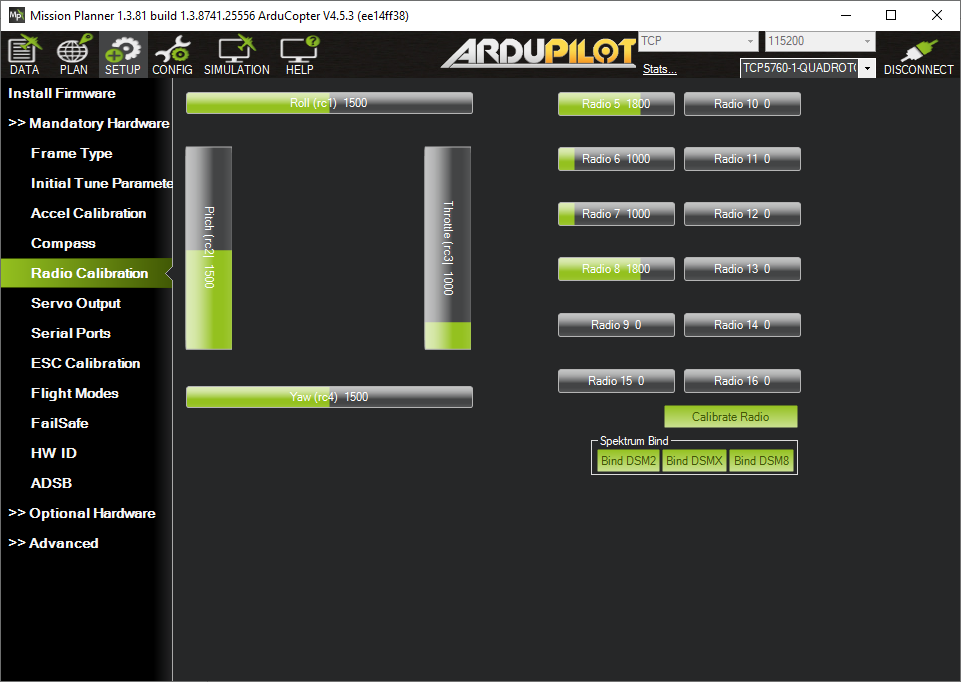
\includegraphics[width=0.8\linewidth]{imagenes/radioCont}
	\caption{Menú de calibración del Radio Control}
	\label{fig:radiocont}
\end{figure}

Al colocarnos en esta pestaña, debemos ver que hay barras verdes, si no se encuentran esas barras verdes, hay que verificar el Radio Control.
En esta ventana comprobaremos el mapeo de los canales de transmisión, también las perillas, palancas e interruptores de nuestro control, lo comprobaremos al presionar los botones y mover las palancas, las barras verdes se empezarán a desplazar
Para la calibración del control, pulsaremos el botón de “Calibrate Radio”, presionamos el botón de “Ok” cuando se solicite verificar que el equipo de control del radio esté encendido y las hélices no están conectadas.


\begin{figure}[H]
	\centering
	\includegraphics[width=\linewidth]{imagenes/contrCheck}
	\caption{Calibración del Radio Control.}
	\label{fig:contrcheck}
\end{figure}

Hacer click cuando hayamos terminado. Acabando de configurar, Mission Planner nos mostrará un resumen de los datos calibrados, los valores comunes rondan entre los 1100 para los mínimos y 1900 para los valores máximos.

\begin{figure}[H]
	\centering
	\includegraphics[width=0.5\linewidth]{imagenes/rangos}
	\caption{Valores Rango de los controles.}
	\label{fig:rangos}
\end{figure}

\subsubsection{Verificación del giro de los motores.}

Es importante verificar la dirección de los motores, porque en caso de que algún motor y propela estén en el sentido contrario, el Dron será incapaz de volar y puede provocar algún tipo de accidente.
\begin{figure}[H]
	\centering
	\includegraphics[width=0.7\linewidth]{imagenes/pixhawkIn}
	\caption{Pines de salida Pixhawk (numerados).}
	\label{fig:pixhawkin}
\end{figure} 

Conectamos los cables de alimentación (+), tierra (-) y señal (s) de cada ESC a los pines de salida principales del Dron por número de motor.

Para dirigirnos a la pestaña de:
\textit{Option}\textrightarrow\textit{ Optional Hardware}\textrightarrow \textit{Motor test}.

\begin{figure}[H]
	\centering
	\includegraphics[width=.89\linewidth]{imagenes/motorTest}
	\caption{Pruebas de Motor.}
	\label{fig:motortest}
\end{figure}

\begin{figure}[H]
	\centering
	\includegraphics[width=0.3\linewidth]{imagenes/quadX}
	\caption{Sentido y dirección de los motores con la punta como nuestro norte de nuestro GPS.}
	\label{fig:quadX}
\end{figure}

\begin{figure}[H]
	\centering
	\includegraphics[width=0.9\linewidth]{imagenes/sense}
	\caption{Leyenda para diagramas de orden de motores.}
	\label{fig:sense}
\end{figure}

\begin{figure}[H]
	\centering
	\includegraphics[width=0.5\linewidth]{imagenes/sense2}
	\caption{Sentido de las propelas en sentido horario y antihorario}
	\label{fig:sense2}
\end{figure}

La forma de comprobar que todo esté correcto es dirigirnos la pestaña de pruebas de motores y probar los 4 motores, sabremos que está bien el sentido porque el aire de impulso se sentirá en la parte de abajo del Dron, en caso de que el aire se sienta en la parte de arriba, habrá que corregir el sentido. Puede que al momento de probar el motor se pueda “atascar” o no poder girar, para solucionar el problema es de ayuda subirle el porcentaje de potencia en la misma ventana (\textit{Throttle}).

\subsubsection{Calibración de las controladoras de vuelo (ESC Calibration)}

Las controladoras de vuelo son las encargadas de hacer girar a los motores a la velocidad solicitada para el Dron, la mayoría de las ESC necesitan ser calibradas para que reconozcan los valores mínimos y máximos de los PWM.

Para la correcta calibración,se debe quitar las propelas del Dron, a continuación, pulsamos el botón de “Calibrate ESCs”, después, y colocar el control en su punto máximo de Pitch y el Dron debe estar con la batería conectada.

\begin{figure}[H]
	\centering
	\includegraphics[width=0.5\linewidth]{imagenes/ctr1}
	\caption{Representación del control con el Throttle al máximo.}
	\label{fig:ctr1}
\end{figure}

Después de presionar el botón que da comienzo a la calibración, desconectamos la batería y volveremos a conectar inmediatamente hasta escuchar los pitidos de confirmación de calibración, cuando escuchemos los pitidos de confirmación, bajaremos la palanca y se procede a la captura del punto mínimo.

\begin{figure}[h]
	\centering
	\includegraphics[width=0.5\linewidth]{imagenes/ctr2}
	\caption{Representación del control con el Throttle al mínimo.}
	\label{fig:ctr2}
\end{figure}

Se escucharán los pitidos de confirmación de la calibración. Al terminar, se escuchará un pitido largo.
Para salir del modo de calibración de la controladora de vuelo, únicamente se desconecta la batería y se vuelve a conectar, esto hará que se salga del modo de configuración.

\subsection{Modos de vuelo.}

Los modos de vuelo programados en el Radio Control son los que utilizamos en las pruebas de vuelo. Como comentario inicial, la palanca del Throttle (Palanca izquierda del control)  siempre debe coincidir que esté completamente hacia abajo, la otra palanca se mantiene en su lugar.

\begin{figure}[h]
	\centering
	\begin{minipage}[b]{0.4\textwidth}
		\centering
		\includegraphics[width=\textwidth]{imagenes/ctr3}
	\end{minipage}
	\hspace{0.05\textwidth} % Espacio entre las dos imágenes
	\begin{minipage}[b]{0.5\textwidth}
		\centering
		\includegraphics[width=1.1\textwidth]{imagenes/mp1}
	\end{minipage}
	\caption{Inicio del primer modo de vuelo, modo “Stabilize”.}
	\label{fig:modo_stabilize}
\end{figure}
\newpage
En el primer modo de vuelo, lo llamaremos “Stabilize”, es el modo con las lengüetas (A, B, C y D) están totalmente hacia arriba, es el modo en que podemos controlar al Dron de una forma completamente manual y la primera parte para empezar el vuelo automático.
El modo de vuelo en automático se establece cuando la lengüeta B se baja en su totalidad.

\begin{figure}[H]
	\centering
	\begin{minipage}[b]{0.4\textwidth}
		\centering
		\includegraphics[width=\textwidth]{imagenes/ctr4}
	\end{minipage}
	\hspace{0.05\textwidth} % Espacio entre las dos imágenes
	\begin{minipage}[b]{0.5\textwidth}
		\centering
		\includegraphics[width=1.1\textwidth]{imagenes/mp2}
	\end{minipage}
	\caption{Modo de vuelo “Auto”.}
	\label{fig:modo_stabilize}
\end{figure}


Para empezar el modo de vuelo automático, se sigue el siguiente procedimiento:
\begin{enumerate}
	\item Primero, subimos el plan de vuelo al Dron.
	\item Poner el control en modo Stabilize.
	\item Se arma el Dron, este paso movemos la palanca del Throttle totalmente hacia abajo y la movemos a la derecha, es importante notar que las calibraciones y el botón de seguridad del Dron debe estar desactivado.
	
	\begin{figure}[H]
		\centering
		\begin{minipage}[b]{0.4\textwidth}
			\centering
			\includegraphics[width=\textwidth]{imagenes/ctr5}
		\end{minipage}
		\hspace{0.05\textwidth} % Espacio entre las dos imágenes
		\begin{minipage}[b]{0.5\textwidth}
			\centering
			\includegraphics[width=1.1\textwidth]{imagenes/mp3}
		\end{minipage}
		\caption{Armado del Dron con la palanca del Throttle.}
		\label{fig:modo_stabilize}
	\end{figure}
	\item Una vez armado el Dron, se pone en modo Auto y se levanta ligeramente la palanca del Throttle y el plan de vuelo comienza a ejecutarse.
\end{enumerate}

Por último, contamos con el modo de vuelo de \textit{“Land”}, este modo es únicamente para el aterrizaje del Dron. Para colocar el Dron en este modo, pasamos del modo Auto al modo Land, bajamos la lengüeta B y seguido subimos la lengüeta A.

	\begin{figure}[H]
	\centering
	\begin{minipage}[b]{0.4\textwidth}
		\centering
		\includegraphics[width=\textwidth]{imagenes/ctr6}
	\end{minipage}
	\hspace{0.05\textwidth} % Espacio entre las dos imágenes
	\begin{minipage}[b]{0.5\textwidth}
		\centering
		\includegraphics[width=1.1\textwidth]{imagenes/mp4}
	\end{minipage}
	\caption{Modo de vuelo “Land”.}
	\label{fig:modo_stabilize}
\end{figure}

El Dron empezará a aterrizar en la posición en que se encuentra.
Para las pruebas que hicimos, se presentaban problemas de lectura con el GPS externo del Dron, por lo que perdía su posición y en muchos casos el Dron hacía un aterrizaje forzado y algunos componentes presentaban descomposturas, por eso, al momento de hacer las pruebas de vuelo, el piloto debe estar atento a los movimientos del Dron en caso de alguna pérdida de lectura del GPS o cambios de velocidad del viento bruscos.

Para controlar que el Dron tenga un buen aterrizaje en caso de alguna falla sin causar daños, tenemos dos opciones de aterrizaje.

\begin{enumerate}
	\item \textbf{Opción de aterrizaje por modo Land:} Es mover el modo de vuelo de \textit{Stabilize} \textrightarrow \textit{Land} o de \textit{Auto} \textrightarrow \textit{Land}, ajustando la palanca del movimiento (Palanca de la Derecha del Control) para evitar la colisión con algún objeto.
	\item  \textbf{Opción de vuelo Manual:} Esta opción es poco recomendada, la opción aplica del modo \textit{Land} \textrightarrow \textit{Stabilize} o del modo \textit{Auto} \textrightarrow \textit{Stabilize}, el piloto toma el control total del Dron, lo que implica tener un excelente control con las palancas de Throttle y de Movimiento, ya que si la palanca de Throttle está totalmente hacia abajo, los motores se apagan y el Dron caerá, por lo que se tiene que tener en una posición adecuada la palanca del Throttle para hacer un descenso lento y controlado.
\end{enumerate}

En cualquier caso, el piloto debe contar con experiencia con el control manual y el control automático del Dron.

\subsection{Planes de Vuelo.}

Los planes de vuelo se personalizan desde la pestaña en Plan.

\begin{figure}[h]
	\centering
	\includegraphics[width=\linewidth]{imagenes/pv1}
	\caption{Pestaña de creación de los planes de vuelo.}
	\label{fig:pv1}
\end{figure}

En la derecha del panel encontramos las opciones de guardar y cargar los planes de vuelo, así como de leer el plan que tiene el Dron y mandarlo a la Memoria del Dron.

Las órdenes que más comúnmente usamos son las siguientes:

\begin{itemize}
	\item Land: Para aterrizaje.
	\item Takeoff: Para despegue del Dron, contiene el parámetro de altura.
	\item Waypoint: El waypoint es un punto al cual queremos que se dirija el Dron, contiene un parámetro para el tiempo de espera dentro del waypoint y la altitud que debe tomar el Dron llegado al punto.
	\item Conditional Yaw: Esta instrucción hace que el Dron gire y se perfile con respecto al norte geográfico, esta opción la colocamos siempre después de la instrucción de takeoff y waypoints para mantener el Dron apuntando hacia el norte.
	
\end{itemize}

Hay más acciones que se pueden tomar para los planes de vuelo para poder hacer más experimentos y observar su comportamiento. Una vez creado el plan de vuelo, el Dron debe estar conectado a través de la telemetría al software de Mission Planner, pulsamos el botón de Write, y el plan estará listo para ejecutarse.

\subsection{Condiciones climatológicas.}
Para tener en cuenta un plan de vuelo, se deben tener las siguientes consideraciones climáticas:
\begin{itemize}
	\item Viento: Se recomienda según blogs [3] tener una velocidad de entre 10 mph a 15 mph, lo que es equivalente de 16 $km/h$ a 24 $km/h$.
	\item Precipitación: Debemos planear el vuelo con nula precipitación o una probabilidad menor o igual al 40\%, según recomendaciones de la aplicación \textit{“UAV Forecast”.}
	\item Cantidad de satélites disponibles: Como recomendación por la misma aplicación UAV Forecast, se recomiendan un mínimo de 8 satélites GPS, incluyendo los satélites GLONASS.
\end{itemize}


\begin{figure}[htbp]
	\centering
	\begin{minipage}[b]{0.3\textwidth}
		\centering
		\includegraphics[width=\textwidth]{imagenes/app1}
		\caption*{Inicio de la aplicación.}
	\end{minipage}
	\hspace{0.02\textwidth} % Espacio entre las imágenes
	\begin{minipage}[b]{0.3\textwidth}
		\centering
		\includegraphics[width=\textwidth]{imagenes/app2}
		\caption*{Probabilidad de precipitación}
	\end{minipage}
	\hspace{0.02\textwidth} % Espacio entre las imágenes
	\begin{minipage}[b]{0.3\textwidth}
		\centering
		\includegraphics[width=\textwidth]{imagenes/app3}
		\caption*{Cantidad de satélites visibles}
	\end{minipage}
	\caption{Aplicación de ayuda para condiciones de vuelo}
	\label{fig:flight_conditions_app}
\end{figure}

Una vez comprobadas las condiciones climáticas apropiadas para el vuelo, se puede proceder a crear el plan de vuelo y a ejecutarlo.


















\section{Implementación de la WSN}
\subsection{Adquisición de los Elementos}
En esta etapa, se procederá con la adquisición de los elementos esenciales para la implementación de la WSN, basándonos en las selecciones detalladas durante el análisis y diseño del proyecto:
\begin{enumerate}
    \item \textbf{Termistor LM35 (temperatura):} Utilizado para monitorear la temperatura ambiental y su análisis podría indicar algún impacto en el comportamiento de las especies.
    \item \textbf{Módulo GPS Neo-6M (geolocalización):} Necesario para rastrear y registrar la ubicación geográfica precisa de las especies, proporcionando información vital sobre la distribución espacial y migración de las especies.
    \item \textbf{Cámara Trampa PR-700 (video): } Esencial para obtener imágenes de alta resolución que facilitarán la identificación de especies y el análisis de su actividad y comportamientos.
    \item \textbf{Arduino Pro Micro (microcontrolador):} Elegido por su bajo consumo energético, capacidad suficiente para tareas específicas del proyecto y tamaño compacto.
    \item \textbf{Módulos LoRa UART 868/915 MHz (transmisión de datos):} Seleccionados por su capacidad única para proporcionar conectividad confiable a larga distancia con bajo consumo de energía.
    \item \textbf{Baterías LiPo recargables (fuente de energía):} Seleccionadas por su buen funcionamiento y larga duración, ofreciendo una solución confiable para dispositivos de monitoreo autónomos.
    \item \textbf{Módulo MicroSD Card Adapter MLMSD (adaptador):} Elegido por su compatibilidad con tarjetas MicroSD, proporcionando capacidades de almacenamiento significativas y fácil integración con microcontroladores.
    \item \textbf{Memorias MicroSD (almacenaje de datos):} Utilizadas para el almacenamiento de datos generados por los sensores y archivos de video de las cámaras trampa.
\end{enumerate}
A continuación, se presenta la tabla comparativa \ref{tabla:precioswsn} que resume los precios y proveedores de cada elemento necesario, con su respectivo hipervínculo:

\begin{table}[H]
  \centering
  \caption{Comparación de precios de componentes electrónicos}
  \begin{tabular}{|l|l|l|l|}
    \hline
    \cellcolor[HTML]{C0C0C0}\textbf{Elemento} & \cellcolor[HTML]{C0C0C0}\textbf{Amazon} & \cellcolor[HTML]{C0C0C0}\textbf{Mercado Libre} & \cellcolor[HTML]{C0C0C0}\textbf{AliExpress} 
    \\ \hline
    Arduino Pro Micro & \$243.00 [\href{https://www.amazon.com.mx/Arduino-Nano-Every-Single-Board/dp/B07VX7MX27/ref=sr_1_3?__mk_es_MX=%C3%85M%C3%85%C5%BD%C3%95%C3%91&crid=307WLXDB631RV&dib=eyJ2IjoiMSJ9.wzfOzm2PL4-zMZ2NN_5BNdR4mDrlSoSOwDLjWcQn9VI4HLku1uxkwYmK6IsZr0xutdI9rmfjBP6GgqhL1reGWB8UoHG6Od8i3xY89uacfvcPGP6-V-2P9SODLnx_0QMijWGI0iT89I0QFjZN9QNvkmCBkQp29V-JNl8GAy2cjAGWzRCRvh0jf78M0DHjbvdrbVZGE2n4M46X2HsC9Nby-mmLOzduvvx3IfTJWFX3ZEhJKyJZxuH06SEP12uh4KzFa9VwFyrzpoqp8bpKrSc5nTBClJrSTum85Uz8CvnsVZE.gSmbVutZeovDlO7E4ayAcklEYu1di6ULkI-0w1CPP38&dib_tag=se&keywords=Arduino%2BPro%2BMicro&qid=1710144626&sprefix=arduino%2Bpro%2Bmicro%2Caps%2C252&sr=8-3&ufe=app_do%3Aamzn1.fos.4e545b5e-1d45-498b-8193-a253464ffa47&th=1}{Amazon}] & \$175.50 [\href{https://articulo.mercadolibre.com.mx/MLM-1941648223-tarjeta-leonardo-pro-micro-16mhz-5v-compatible-con-arduino-_JM#position=6&search_layout=stack&type=item&tracking_id=00e5ebad-5e49-4afc-bd81-e6c056af7411}{Mercado Libre}] & \$65.09 [\href{https://es.aliexpress.com/item/1005005234161130.html?spm=a2g0o.productlist.main.3.4980Q434Q434c4&algo_pvid=7d1f91e3-002d-456e-9407-d23756667968&aem_p4p_detail=2024031101101816580952553541430004787116&algo_exp_id=7d1f91e3-002d-456e-9407-d23756667968-1&pdp_npi=4%40dis%21MXN%2165.09%2165.09%21%21%213.80%213.80%21%402101fb1417101446189377471e211f%2112000032305530340%21sea%21MX%210%21AB&curPageLogUid=d7dvSAouEC8o&utparam-url=scene%3Asearch%7Cquery_from%3A&search_p4p_id=2024031101101816580952553541430004787116_2}{AliExpress}] \\ \hline
    Termistor LM35 & \$40.00 [\href{https://www.amazon.com.mx/Precision-Centigrade-Temperature-Sensors-original/dp/B07VZ567YJ/ref=sr_1_8?__mk_es_MX=%C3%85M%C3%85%C5%BD%C3%95%C3%91&crid=130LLR8OJMASG&dib=eyJ2IjoiMSJ9.jFfBJnZAJqV6Q6JweL1uxoGmt6vmVyVuMFf6ko5tbTh9M3i2NMnBBzqp83CvScdrxLixD41-Tu1nc_9rcKxUvnXySlsrbJtx-4kXTDFVwhCZLLo-om2UFoZiRr6znJm5PUfpUR6-TunS0olQH4R2WYhnhfVNcZdFG6YAYmDepTf5S_y8VVKvmCgI4Ch5QBeH1wpHS6oKOJ7w6gn5o4xkH_37O1hsPXs18Hjbx0WMuFggfkwDUGREEOOH3Kfir_xlPK4GzZkCftaVdslRgQh-jj00S8cy4TwL18Ps1-US8M0.J1_A7vUWx5dlHfUiQUYMtFrIr4oNVspGhi0ZarDJznk&dib_tag=se&keywords=Termistor+LM35&qid=1710143659&sprefix=termistor+lm35%2Caps%2C207&sr=8-8}{Amazon}] & \$63.50 [\href{https://articulo.mercadolibre.com.mx/MLM-839463622-sensor-de-temperatura-lm35-dz-_JM#position=32&search_layout=grid&type=item&tracking_id=d6f18b96-6c7c-47c4-8ed0-cef8096f5927}{Mercado Libre}] & \$25.86 [\href{https://es.aliexpress.com/item/1005004825930346.html?spm=a2g0o.productlist.main.39.50cdprYxprYxX7&algo_pvid=91a52733-c6a4-4fc3-b3c8-fe28fdf689eb&aem_p4p_detail=202403110057211467828156373050004809487&algo_exp_id=91a52733-c6a4-4fc3-b3c8-fe28fdf689eb-19&pdp_npi=4%40dis%21MXN%2131.51%2125.86%21%21%211.84%211.51%21%402101fb1417101446189377471e211f%2112000032305530340%21sea%21MX%210%21AB&curPageLogUid=d7dvUmDO4G8x&utparam-url=scene%3Asearch%7Cquery_from%3A&search_p4p_id=202403110057211467828156373050004809487_2}{AliExpress}] \\ \hline
    Módulo GPS Neo-6M & \$119.00 [\href{https://www.amazon.com.mx/Neuftech-NEO-6M-GPS-Receiver-STM32-Arduino/dp/B01MYVG3P5/ref=sr_1_3?__mk_es_MX=%C3%85M%C3%85%C5%BD%C3%95%C3%91&crid=1TFZ78IGIQNVF&dib=eyJ2IjoiMSJ9.-i5lTPNtYdUCJy1dxg7GJxYQFmQ3KgpnoyKhLQmb57X5PndCaxvg2Id-Tmo8V4xlxNGaRksD_ySuQ9CHP_2zHtCbXnlmbFLC04dvwHhdN_4EkkPQGNEwqXlHoQg2-jKLz_MLRCb9SD5hWiAlzSuvxuGHZyjw7bfu1KLVVtLIhigfRXbpPANmEGSV9JZr8wB9nEnl9k4Rhw9hCrThrl4X4uXyNhT_4fyj0qMTiFRCY7-_RWSzRf-yYr82Iw9GLapxrPh4J3zXWQUVT6W_4L_gDudLF7dWkPlu4e5x7RYTTrQz5TjH8RicX9_XeVwwE.DsWg90xkz47l8wzHOG5iYVwnTDE1E-EmXCIRX3R06ZM&dib_tag=se&keywords=NEO-6M&qid=1710143727&sprefix=neo-6m%2Caps%2C201&sr=8-3}{Amazon}] & \$149 [\href{https://articulo.mercadolibre.com.mx/MLM-677336119-modulo-gps-neo-6m-gy-gps6mv2-para-arduino-pic-raspberry-pi-_JM#position=4&search_layout=stack&type=item&tracking_id=00e5ebad-5e49-4afc-bd81-e6c056af7411}{Mercado Libre}] & \$72.62 [\href{https://es.aliexpress.com/item/1005004438292781.html?spm=a2g0o.productlist.main.1.2cfb4b1cU5qbmZ&algo_pvid=91a52733-c6a4-4fc3-b3c8-fe28fdf689eb&aem_p4p_detail=202403110057211467828156373050004809487&algo_exp_id=91a52733-c6a4-4fc3-b3c8-fe28fdf689eb-1&pdp_npi=4%40dis%21MXN%2172.62%2172.62%21%21%215.85%215.85%21%402101fb1417101446189377471e211f%2112000032305530340%21sea%21MX%210%21AB&curPageLogUid=d7dvUmDO4G8x&utparam-url=scene%3Asearch%7Cquery_from%3A&search_p4p_id=202403110057211467828156373050004809487_2}{AliExpress}] \\ \hline
    Cámara Trampa PR-700 & \$1,309.64 [\href{https://www.amazon.com.mx/1080P-Trail-Camara-Caza-Vision/dp/B07R7Z5X12/ref=sr_1_1?__mk_es_MX=%C3%85M%C3%85%C5%BD%C3%95%C3%91&crid=1R0S82IBX5JLD&dib=eyJ2IjoiMSJ9.MDHzttm1r5hzXwqff8s0xXxtbVtC7Y5dSLr4ejodQOFXRYgRUdZsTBe1f14ZB-0nxYIhnb3qPzsjGg1XzQjeUXm1NwP9z-TlkiWFOqHtw9f9ImSyRA05do-IwevGMD6nUTR-Bfl-vS55JNrswUiyHb_1TyPK5vo6W-79L-zA4vqIAbJ6ZcGWbbYri__vsf-Jb0Ku6yigXT1G4AqkZ5X2-nwGb0Bd4ujXQKd_2tECmk7bPJ5JKSYLpRlBndVV7xJP7qIr1tpXUyoGocGfF-LgXXHwTq4xFw.4Hk_y6TZTQjyVm2vzfrN9wJkv8aFZoZszn7EwULtqVg&dib_tag=se&keywords=c%C3%A1mara+trampa&qid=1710144371&sprefix=c%C3%A1mara+tra%2Caps%2C243&sr=8-1}{Amazon}] & \$770.65 [\href{https://articulo.mercadolibre.com.mx/MLM-657680742-camara-trampa-hc801g-16mp-celular-infrarrojo-piezo-gsm-1080p-_JM#position=1&search_layout=grid&type=item&tracking_id=00e5ebad-5e49-4afc-bd81-e6c056af7411}{Mercado Libre}] & \$234.37 [\href{https://es.aliexpress.com/item/1005003196329359.html?spm=a2g0o.productlist.main.5.26d34717R8y5R9&algo_pvid=eb8c5605-2939-4b13-bc4b-9a3e07e7a2ec&aem_p4p_detail=202403110057211467828156373050004809487&algo_exp_id=eb8c5605-2939-4b13-bc4b-9a3e07e7a2ec-1&pdp_npi=4%40dis%21MXN%21234.37%21234.37%21%21%2111.78%2111.78%21%402101fb1417101446189377471e211f%2112000032305530340%21sea%21MX%210%21AB&curPageLogUid=d7dvUmDO4G8x&utparam-url=scene%3Asearch%7Cquery_from%3A&search_p4p_id=202403110057211467828156373050004809487_2}{AliExpress}] \\ \hline
    Módulos LoRa & \$353.50 [\href{https://www.amazon.com.mx/DRF1278DM-WX-DRF1278DM-WX915-Long-Range-Transceiver/dp/B07VTVV8G8/ref=sr_1_6?__mk_es_MX=%C3%85M%C3%85%C5%BD%C3%95%C3%91&crid=11JCGW93RMYOS&dib=eyJ2IjoiMSJ9.jxvL2e6CxkW43ZbNjNLjGTD0M9Nx9sRerR6vmj1f18CvF3I-dYRzsUV0PIcArbFtsDVQqHswC7kKZWKhL5EkulL-tO-1fb7g-15mT83wlJaR3Ek3uzUX_vuUw-T1a1wHThp00X3ZxHIdin-l_7cHWhM0yrzBB-0vYwKbgqXCE1s6-02EPR3rIf6x6hFkG8vS0otzdB-k55x53uOKMv0jKpjGb-Wog7C-r4j4rVLaIiS2ot5j5qoFDb1aI6qBKQ5pbNLpCJbqSBL-J0PLtXU-cISbGnGIEfA_HD4YJEI.UhbZ9O-8jJKf0C6VCpx8xeqkIMATBGVTszA5u5gkFbg&dib_tag=se&keywords=m%C3%B3dulo+lora&qid=1710144415&sprefix=m%C3%B3dulo+lora%2Caps%2C246&sr=8-6}{Amazon}] & -------------------- & \$59.09 [\href{https://es.aliexpress.com/item/1005005041209461.html?spm=a2g0o.productlist.main.2.4bba8a17dAjEJY&algo_pvid=09177cb8-446f-400e-8dd7-f5a29445c92a&aem_p4p_detail=2024031101101816580952553541430004787116&algo_exp_id=09177cb8-446f-400e-8dd7-f5a29445c92a-0&pdp_npi=4%40dis%21MXN%2159.09%2159.09%21%21%212.66%212.66%21%402101fb1417101446189377471e211f%2112000032305530340%21sea%21MX%210%21AB&curPageLogUid=d7dvSAouEC8o&utparam-url=scene%3Asearch%7Cquery_from%3A&search_p4p_id=2024031101101816580952553541430004787116_2}{AliExpress}] \\ \hline
    Módulo adaptador MicroSD & \$22.99 [\href{https://www.amazon.com.mx/LEORX-Adaptador-conector-micro-SD-convertidor/dp/B01189N29A/ref=sr_1_4?__mk_es_MX=%C3%85M%C3%85%C5%BD%C3%95%C3%91&crid=2IE9B9Q0K0FHZ&dib=eyJ2IjoiMSJ9.f0jv3XQ9CzoKyZsvCBJfHkVHwMW-ZfFImHJf9SeVJ5pjACk94RysWYNFvx1_CZrXVbSMaUmoPxeSyVhNpN9HfWQptqxpruWyNLE8Y4klz6UPXbHrPy49fULGOv3zUErFkfBqvoiIcV3tkhdFbX1QJUaFwjD6u9QDK8qP6i7B6Ki5XGh6wbe1Wv8l7NRD3k-3_zwO8gGe8qBn32eWXU6x9vUfFe8kLQ1wFR8MNSzjr5AZxrf9oTfBf9HHo-F72nQMdRwNkKEI2g2JkVUK0zw-1QUk.d1D8vKwnF2zncIEQ7QLx2lwIJ7jPftAOnaAYw1Zm1F8&dib_tag=se&keywords=adaptador+micro+sd&qid=1710144466&sprefix=adaptador+mic%2Caps%2C229&sr=8-4}{Amazon}] & \$43.60 [\href{https://articulo.mercadolibre.com.mx/MLM-652437431-adaptador-micro-sd-a-micro-sd-microsd-otg-tablet-android-_JM#position=1&search_layout=stack&type=item&tracking_id=00e5ebad-5e49-4afc-bd81-e6c056af7411}{Mercado Libre}] & \$6.17 [\href{https://es.aliexpress.com/item/1005004858720352.html?spm=a2g0o.productlist.main.20.1bda5712ji8NoH&algo_pvid=7d1f91e3-002d-456e-9407-d23756667968&aem_p4p_detail=2024031101101816580952553541430004787116&algo_exp_id=7d1f91e3-002d-456e-9407-d23756667968-8&pdp_npi=4%40dis%21MXN%216.17%216.17%21%21%212.90%212.90%21%402101fb1417101446189377471e211f%2112000032305530340%21sea%21MX%210%21AB&curPageLogUid=d7dvSAouEC8o&utparam-url=scene%3Asearch%7Cquery_from%3A&search_p4p_id=2024031101101816580952553541430004787116_2}{AliExpress}] \\ \hline
    Memorias MicroSD & \$54.50 [\href{https://www.amazon.com.mx/LEORX-Tarjeta-micro-SD-16-32GB/dp/B017JU1PCO/ref=sr_1_6?__mk_es_MX=%C3%85M%C3%85%C5%BD%C3%95%C3%91&crid=2I8A93F4UCOHB&dib=eyJ2IjoiMSJ9.mjoSQwypHnBhx8ABz7L1CgIGopvjGQW-xdK7EZ6Z_YiIlMDv3Vsn7Qj4LkllcrdOlZlsmnG2hncwY3Pw12EzoIGnIZe7ZcLVNlPvd3uPfsALIEiiN9JznBWXIn4fbTHWXkVO7dLzH5ZmCwrAB2fsEr3TmCxI2H5b-p8HJO8DBoSVjnC8EdXROJ0rfrnEZ66G0dH5MTsfhG8RiNYIe9dWHEMwriMUEelWs3cC1DEo2ec1WeAQgH6ouWc4NMo2HNWc-aar4o3DkFNdYAQ.1xmIPIWVLn_M3-mYbPvCIBayZdCDzHv-jE03pTQLN2w&dib_tag=se&keywords=memoria+micro+sd&qid=1710144518&sprefix=memoria+mic%2Caps%2C238&sr=8-6}{Amazon}] & \$72.00 [\href{https://articulo.mercadolibre.com.mx/MLM-630745934-memoria-micro-sd-32gb-clase-10-kingston-original-envio-gratis-_JM#position=3&search_layout=stack&type=item&tracking_id=00e5ebad-5e49-4afc-bd81-e6c056af7411}{Mercado Libre}] & \$63.54 [\href{https://es.aliexpress.com/item/1005004748254670.html?spm=a2g0o.productlist.main.32.4bba8a17dAjEJY&algo_pvid=eb8c5605-2939-4b13-bc4b-9a3e07e7a2ec&aem_p4p_detail=202403110057211467828156373050004809487&algo_exp_id=eb8c5605-2939-4b13-bc4b-9a3e07e7a2ec-14&pdp_npi=4%40dis%21MXN%2163.54%2163.54%21%21%212.60%212.60%21%402101fb1417101446189377471e211f%2112000032305530340%21sea%21MX%210%21AB&curPageLogUid=d7dvUmDO4G8x&utparam-url=scene%3Asearch%7Cquery_from%3A&search_p4p_id=202403110057211467828156373050004809487_2}{AliExpress}] \\ \hline
    Batería (1200mAh 3.7v 103040) & \$110.02 [\href{https://www.amazon.com.mx/LYD-Battery-Bater%C3%ADa-recargable-Lithium-Polymer/dp/B07W5MPCPN/ref=sr_1_5?__mk_es_MX=%C3%85M%C3%85%C5%BD%C3%95%C3%91&crid=2LXWTJW6IQIWX&dib=eyJ2IjoiMSJ9.E0ZXCzYKrsQXfnf-s5t1VvWSlBxzOrZnwmU4Xu0STYEOgibKTIlInOT2n7t1DYTak7fyYGKg4fWFlc01SACOp2AF-C7UIGnWkjA9N1rE8s6KzP9nXRTJQb_DnsFCzq-PdoJEPKshkoHix6Cmbj_gexK7Hxgq7uUp3BNLZbyhA9jZiL8G6Wm7rNcEDmN3WW3ZXkGxZ1QJAZe1u2cxNp4o_3P3Hb9kVknHc4hIkz9swb5dNNpsnGq-y3OeMQo_qo_BiabgUV6pypO3zUSNnqTZ1A.TTr3CPjSf_iqMLwK9lmD9a-tDk47KAGs7orB4SytQQI&dib_tag=se&keywords=bater%C3%ADa+3.7v&qid=1710144593&sprefix=bater%C3%ADa+3.7v%2Caps%2C252&sr=8-5}{Amazon}] & \$110.02 [\href{https://articulo.mercadolibre.com.mx/MLM-899787949-bateria-lipo-lion-de-litio-37v-1200mah-103040-_JM#position=1&search_layout=grid&type=item&tracking_id=00e5ebad-5e49-4afc-bd81-e6c056af7411}{Mercado Libre}] & \$71.60 [\href{https://es.aliexpress.com/item/1005004568769731.html?spm=a2g0o.productlist.main.5.4bba8a17dAjEJY&algo_pvid=eb8c5605-2939-4b13-bc4b-9a3e07e7a2ec&aem_p4p_detail=202403110057211467828156373050004809487&algo_exp_id=eb8c5605-2939-4b13-bc4b-9a3e07e7a2ec-9&pdp_npi=4%40dis%21MXN%2171.60%2171.60%21%21%2111.77%2111.77%21%402101fb1417101446189377471e211f%2112000032305530340%21sea%21MX%210%21AB&curPageLogUid=d7dvUmDO4G8x&utparam-url=scene%3Asearch%7Cquery_from%3A&search_p4p_id=202403110057211467828156373050004809487_2}{AliExpress}] \\ \hline
  \end{tabular}
  \label{tabla:precioswsn}
  \caption*{Nota: Los precios indicados son en la moneda mexicana, los cuales junto con la disponibilidad de los productos pueden variar con el tiempo.}
\end{table}
A continuación, se muestran las imágenes de los elementos adquiridos para la implementación de la WSN. Estas imágenes proporcionarán una visualización clara de los componentes seleccionados y facilitarán la identificación y verificación de los elementos.
\begin{figure}[H]
    \centering
    \begin{minipage}{\textwidth}
        \centering
        \begin{minipage}{\textwidth}
            \centering
            \subfigure[) Arduino Pro Micro.]{\includegraphics[width=0.45\textwidth]{imagenes/elemento-arduino.jpeg}}
            \label{fig:arduino_pro_micro}
            \subfigure[) Termistor LM35.]{\includegraphics[width=0.3\textwidth, height=4.2cm]{imagenes/elemento-termistor.jpeg}}
            \label{fig:lm35_termistor}
        \end{minipage}
    \end{minipage}
\end{figure} 

\begin{figure}[H]
\begin{minipage}{\textwidth}
\centering
\begin{minipage}{\textwidth}
\centering
\subfigure[) GPS Neo-6M.]{\includegraphics[ height=6cm]{imagenes/elemento-gps.jpeg}}
\label{fig
}
\subfigure[) Transceptor LoRa.]{\includegraphics[ height=6cm]{imagenes/elemento-lora.jpg}}
\label{fig
}
\end{minipage}
\end{minipage}
    
    \begin{minipage}{\textwidth}
        \centering
        \begin{minipage}{\textwidth}
            \centering
            \subfigure[) Batería LiPo de 3.7V.]{\includegraphics[ height=5cm]{imagenes/elemento-bateria.jpeg}}
            \label{fig:lipo_battery}
            \subfigure[) Cámara PR-700.]{\includegraphics[ height=5cm]{imagenes/elemento-camara.jpeg}}
            \label{fig:pr_700_camera}
        \end{minipage}
    \end{minipage}
    
    \caption{Elementos adquiridos para la WSN.}
    \label{fig:wsn_elements}
\end{figure}


\subsection{Funcionamiento de los Elementos}
Una vez adquiridos todos los elementos necesarios para la implementación de la WSN, se verificará su funcionamiento. Esta etapa garantizará que cada componente funcione correctamente y esté listo para su integración en el sistema. A continuación, se describen los pasos para verificar el funcionamiento de cada elemento:
\begin{itemize}
    \item \textbf{Arduino Pro Micro:}
    
Se conecta el Arduino Pro Micro a un puerto USB disponible en el ordenador mediante un cable USB adecuado y se verifica que el LED de alimentación del Arduino Pro Micro se encienda, lo que indica que está recibiendo energía correctamente.

Se carga un programa de prueba simple en el Arduino Pro Micro utilizando el entorno de desarrollo Arduino IDE. Este programa puede ser tan básico como hacer parpadear el LED interno del Arduino cada segundo.

Se observa el comportamiento del Arduino Pro Micro para confirmar que responde correctamente al programa cargado. Se espera que el LED conectado parpadee según lo programado, lo que indica que el Arduino está funcionando correctamente.
\begin{figure}[H]
    \centering
    \includegraphics[width=0.6\textwidth]{imagenes/prueba-led.jpeg}
    \caption{Prueba del led interno de Arduino Pro Micro.}
    \label{fig:prueba_led_arduino}
\end{figure}

\item \textbf{Termistor LM35:}

El termistor LM35 se conecta a la placa Arduino según las especificaciones del fabricante. Se conecta el pin de salida del termistor al pin analógico de lectura de la placa Arduino (por ejemplo, A0), el pin VCC del termistor al pin de 5V de la placa Arduino, y el pin GND del termistor al pin de tierra (GND) de la placa Arduino.

Para probar su funcionamiento, se desarrolla un programa en el entorno de desarrollo Arduino IDE para leer la temperatura ambiente mediante el termistor LM35. Este programa realiza la lectura del valor analógico del pin conectado al termistor y lo convierte a temperatura en grados Celsius utilizando la fórmula proporcionada por el datasheet del LM35, la cual es: $\text{T[°C]} = \left( \frac{\text{valorSensor} \times 5}{1023} \right) \times 100$ .  

Una vez cargado el programa en la placa Arduino, se puede verificar la correcta lectura de la temperatura ambiente. Si se coloca el termistor en un entorno con una temperatura conocida y se observa la salida del monitor serial en el Arduino IDE. Se pueden comparar las lecturas obtenidas con la temperatura ambiente medida independientemente para verificar la precisión del termistor en la medición de la temperatura.

\begin{figure}[H]
    \centering
    \includegraphics[width=0.5\textwidth, height=4cm]{imagenes/temperatura_solo.jpg}
    \caption{Resultado de registrar la temperatura del termistor LM35.}
    \label{fig:temp-solo}
\end{figure}

\begin{figure}[H]
    \centering
    \includegraphics[width=0.6\textwidth, height=4cm]{imagenes/prueba-termistor.jpeg}
    \caption{Prueba del termistor LM35 usando el Arduino Pro Micro.}
    \label{fig:prueba_termistor}
\end{figure}


\item \textbf{Módulo GPS Neo-6M:}

El módulo GPS Neo-6M se conecta a la placa Arduino siguiendo las especificaciones proporcionadas por el fabricante. Se conecta el pin de datos del módulo GPS (RX) al pin TX de la placa Arduino y el pin de datos (TX) al pin RX de la placa Arduino mediante cables jumper. De igual modo, se conectan los pines VCC y GND del módulo GPS a los pines de alimentación de 5V (VCC) y tierra (GND) de la placa Arduino, respectivamente.

Se desarrolla un programa en el entorno de desarrollo Arduino IDE para configurar el módulo GPS Neo-6M y recibir datos de los satélites para obtener la ubicación actual. El programa establece la comunicación serial con el módulo GPS y envía los comandos AT necesarios para configurar el módulo y solicitar datos de ubicación.

Para la realización de este programa, primeramente se desarrolló y probó en una placa Arduino Uno, utilizando la librería TinyGPS++, esto debido a que se presentaban problemas de comunicación al utilizarlo con un Arduino Pro Micro. Una vez verificado que el programa funcione correctamente en la placa Arduino Uno, que el módulo GPS adquiera señales de satélite y que proporcione datos precisos de ubicación, se procedió a ajustar la velocidad de comunicación del módulo para que fuera compatible con el Arduino Pro Micro.

Esto mediante un nuevo programa encargado de configurar la velocidad de comunicación del módulo GPS Neo-6M a través del envío de un comando específico (\$PMTK251,9600*17). Luego, en el bucle principal, se lee la información proporcionada por el módulo GPS y se procesa el mensaje GPRMC para obtener la latitud, la longitud y la hora.

Las coordenadas obtenidas se convierten a formato decimal y se ajustan según el hemisferio y el huso horario para obtener la ubicación exacta y la hora local de la Ciudad de México (GMT-6). Finalmente, se imprimen las coordenadas y la hora en el formato deseado.

Una vez cargado el programa en la placa Arduino, se procede a verificar que el módulo GPS pueda adquirir señales de satélite y proporcionar datos precisos de ubicación. Se coloca el módulo GPS en un lugar abierto y se observa la salida del monitor serial en el Arduino IDE. Se verifican los datos de ubicación proporcionados por el módulo GPS y se comparan con la ubicación conocida para asegurar su precisión.

\begin{figure}[H]
    \centering
    \includegraphics[width=0.75\textwidth, height=4cm]{imagenes/gps_solo.jpg}
    \caption{Resultado de obtener las coordenadas y la hora mediante el GPS-6M.}
    \label{fig:gps-solo}
\end{figure}

\begin{figure}[H]
    \centering
    \subfigure[) Usando el Arduino UNO.]{\includegraphics[width=0.45\textwidth, height=5cm]{imagenes/prueba-gps-uno.jpeg}}
    \quad
    \subfigure[) Usando el Arduino Pro Micro.]{\includegraphics[width=0.45\textwidth, height=5cm]{imagenes/prueba-gps-micro.jpeg}}
    \caption{Prueba del GPS-6M.}
    \label{fig:prueba_gps}
\end{figure}

\item \textbf{Cámara Trampa PR-700:}

La cámara trampa se alimenta con 4 baterías AA (aunque tiene espacio para 8 baterías AA, para utilizar las otras 4 baterías si se llegara a acabar la carga de las primeras 4) o mediante el cable tipo Micro USB que viene incluido, utilizando una fuente de energía adecuada según las especificaciones del fabricante. Asegurándose de que la alimentación sea estable y suficiente para el funcionamiento óptimo de la cámara trampa durante el período de monitoreo.

Se ajustan los parámetros de la cámara trampa, como la resolución de imagen y la frecuencia de disparo, de acuerdo con los requisitos del proyecto, esto mediante el menú de configuración de la cámara trampa.

Después de la configuración, se procede a verificar que la cámara trampa pueda capturar imágenes de alta calidad y almacenarlas en una tarjeta de memoria de tipo MicroSD. Se coloca la cámara trampa en el lugar deseado y se activa para que comience a capturar imágenes. Se revisan las imágenes capturadas para evaluar su calidad y claridad. Se verifica que las imágenes sean nítidas y que capturen adecuadamente archivos multimedia cuando ocurre un movimiento en la zona durante el tiempo preestablecido.

\begin{figure}[H]
    \centering
    \includegraphics[height=7cm]{imagenes/prueba-camara.jpeg}
    \caption{Prueba de la cámara trampa PR-700.}
    \label{fig:prueba_camara_trampa}
\end{figure}


\item \textbf{Módulo LoRa UART 868/915 MHz:}

Se conecta el módulo LoRa a la placa Arduino siguiendo las especificaciones del fabricante. Es crucial asegurar una conexión adecuada para garantizar la comunicación efectiva entre los dispositivos.

Se configura el módulo LoRa para establecer la comunicación con otro módulo LoRa. Esto implica ajustar parámetros como la frecuencia de operación, el factor de propagación y la potencia de transmisión para garantizar una transmisión confiable de datos, utilizando la librería"LoRa\_E22.h", que proporcionan las funciones y definiciones necesarias para la comunicación y el control del módulo LoRa E22. También se configuran los pines utilizados para conectar el Arduino Pro Micro con el módulo LoRa E22, esto incluye los pines de recepción (Rx), transmisión (Tx), AUX (para indicaciones), y los pines M0 y M1 para configurar los modos de funcionamiento del módulo LoRa.

Se realizan pruebas de comunicación entre los módulos LoRa para confirmar la conectividad y la transmisión de datos sin errores. Enviando mensajes desde un módulo LoRa utilizando  la función `sendMessage()' y verificando que sean recibidos correctamente por el otro módulo con  la función `receiveMessage()'. Se realizan múltiples pruebas en diferentes condiciones para garantizar la robustez del sistema de comunicación.

\begin{figure}[H]
	\centering
	\subfigure[Transmisor.]{
		\includegraphics[width=0.37\textwidth, height=4cm]{imagenes/loratx_solo.jpg}
		\label{fig:transmisor}
	}
	\hspace{0.5cm} % Espacio vertical entre las imágenes
	\subfigure[Receptor.]{
		\includegraphics[width=0.37\textwidth, height=4cm]{imagenes/lorarx_solo.jpg}
		\label{fig:receptor}
	}
	\caption{Resultado de transmitir y recibir mediante los transceptores LoRa.}
	\label{fig:lora-solo}
\end{figure}





\begin{figure}[H]
    \centering
    \subfigure[) Transmisor.]{\includegraphics[width=0.45\textwidth, height=5cm]{imagenes/prueba-lora-tx.jpeg}}
    \quad
    \subfigure[) Receptor.]{\includegraphics[width=0.45\textwidth, height=5cm]{imagenes/prueba-lora-rx.jpeg}}
    \caption{Prueba de los módulos LoRa usando Arduinos Pro Micro.}
    \label{fig:prueba_modulos_LoRa}
\end{figure}


\item \textbf{Módulo Adaptador MicroSD y Memorias MicroSD:}

Se inserta una tarjeta MicroSD en el módulo adaptador y se conecta este último a la placa de Arduino Pro Micro. Es importante asegurarse de que la tarjeta esté correctamente insertada. 

Después, se conecta físicamente el módulo adaptador MicroSD a la placa Arduino, siguiendo las siguientes conexiones de acuerdo a la librería utilizada llamada SD: el pin SCK se conecta al pin 15 de la placa (SCK del adaptador), MOSI al pin 16 (MOSI del adaptador), MISO al pin 14 (MISO del adaptador) y el ChipSelect del adaptador a un pin de elección de la placa Arduino Pro Micro(en nuestro caso se configuró el pin 10).

Posteriormente, se realizan pruebas de escritura y lectura de datos desde la tarjeta MicroSD para asegurarse de que la comunicación y el almacenamiento funcionen correctamente. Esto, implementa un menú interactivo en el monitor serial que permite al usuario seleccionar entre las opciones de escritura, lectura o borrado del archivo en la tarjeta MicroSD. Este menú proporciona una forma conveniente de probar las diferentes funciones que se pueden utilizar con la librería SD.

Una vez seleccionada una opción, se ejecuta el proceso correspondiente y se realizan las pruebas necesarias para verificar el correcto funcionamiento de cada función. Durante la escritura, se ingresan datos en el archivo en la tarjeta MicroSD. En el caso de la lectura, se recuperan los datos almacenados y se muestran en el monitor serial para su visualización. Para la opción de borrado, se elimina el archivo de la tarjeta MicroSD. El funcionamiento de este menú se puede observar en la Figura \ref{fig:memoria-solo}.

Después, se retira la tarjeta MicroSD y se coloca en otro dispositivo capaz de leer la tarjeta para así poder verificar la integridad de los datos almacenados. Se comparan estos datos leídos con los datos originales para asegurarse de que no haya errores de lectura o corrupción de datos.

\begin{figure}[H]
    \begin{minipage}{\textwidth}
        \centering
        \begin{minipage}{\textwidth}
            \centering
            \subfigure[) Escribir en el archivo.]{\includegraphics[width=0.45\textwidth, height=4cm]{imagenes/memoria_solo1.jpg}}
            \subfigure[) Leer el archivo.]{\includegraphics[width=0.45\textwidth, height=4cm]{imagenes/memoria_solo2.jpg}}
        \end{minipage}
    \end{minipage}
    \begin{minipage}{\textwidth}
        \centering
        \begin{minipage}{\textwidth}
            \centering
            \subfigure[) Borrar el archivo.]{\includegraphics[width=0.45\textwidth, height=4cm]{imagenes/memoria_solo3.jpg}}
            \subfigure[) Salir del programa.]{\includegraphics[width=0.45\textwidth, height=4cm]{imagenes/memoria_solo4.jpg}}
        \end{minipage}
\end{minipage}
\caption{Resultado de las funciones disponibles del adaptador MicroSD.}
\label{fig:memoria-solo}
\end{figure}

\begin{figure}[H]
    \centering
    \includegraphics[width=0.55\textwidth, height=4.6cm]{imagenes/prueba-adaptador.jpeg}
    \caption{Prueba del adaptador MicroSD usando el Arduino Pro Micro.}
    \label{fig:prueba_adaptador_MicroSD}
\end{figure}


\item \textbf{Baterías LiPo:}

Se utilizan cargadores compatibles para cargar completamente las baterías LiPo. Durante este proceso, se verifica que las baterías acepten la carga y que la tensión de salida sea la esperada mediante el uso de un multímetro.

Una vez que las baterías están completamente cargadas, se mide la tensión de salida para garantizar que esté dentro del rango especificado por el fabricante. Esta medida es crucial para asegurar un suministro de energía estable y confiable al sistema.

Después, se conectan las baterías LiPo al Arduino Pro Micro, asegurándose de que el positivo de la batería se conecte al pin RAW del Arduino y que la tierra se conecte al pin GND. Esta configuración garantiza un suministro de energía adecuado al Arduino y proporciona la conexión eléctrica necesaria para su funcionamiento dentro de la WSN.
\begin{figure}[H]
    \centering
    \includegraphics[width=0.55\textwidth, height=4cm]{imagenes/prueba-bateria.jpeg}
    \caption{Prueba de la batería LiPo para energizar el Arduino Pro Micro.}
    \label{fig:prueba_bateria_LiPo}
\end{figure}


\end{itemize}

Una vez completada la verificación de cada elemento individual, se procederá a la integración de los componentes en la red de sensores inalámbricos. Por lo que es fundamental que cada componente funcione correctamente para garantizar la fiabilidad del sistema en su conjunto.

\subsection{Integración de los Elementos}
Después de haber verificado el funcionamiento de los componentes de manera individual se llevará a cabo su integración. Explorando cómo almacenar los datos de temperatura y GPS en una tarjeta MicroSD para su posterior análisis y cómo utilizar la tecnología LoRa para la transmisión eficiente de estos datos entre nodos de la red. A través de estos procesos de integración, se espera obtener una red de sensores completamente funcional y lista para su despliegue en el campo.
\begin{itemize}
    \item \textbf{Almacenamiento de datos de temperatura en la tarjeta MicroSD:} Se almacenan los datos recopilados por el sensor de temperatura en la tarjeta MicroSD, mediante la conversión de los valores analógicos obtenidos del termistor a grados Celsius y guardándolos junto con una marca de tiempo en un archivo de texto en la tarjeta MicroSD, además se muestran estos datos en el Monitor Serial.

El código realizado comienza inicializando la comunicación serial y configurando un pin para alimentar el termistor directamente, ya que el pin de VCC será utilizado para alimentar el módulo adaptador MicroSD, también se le configura el chip select y se conectan los demás pines como en se vio en el Funcionamiento de los Elementos. Después, se inicializa la tarjeta MicroSD y se borra el archivo de temperatura en caso de ya existir.

En el bucle principal, se lee el valor analógico del termistor, se convierte a temperatura en grados Celsius y se obtiene la marca de tiempo en formato HH:MM:SS iniciando desde el encendido del Arduino utilizando la función millis() de la librería TimeLib. Esta información se muestra en el Monitor Serial y se guarda en un archivo de texto en la tarjeta MicroSD en el siguiente formato: "temperatura; hora".

\begin{figure}[H]
    \centering
    \subfigure[) Monitor Serial.]{\includegraphics[width=0.45\textwidth, height=4cm]{imagenes/temperatura_memoria.jpg}}
    \quad
    \subfigure[) Archivo de texto.]{\includegraphics[height=3cm]{imagenes/temperatura_memoria-txt.jpg}}
    \caption{Resultados de guardar la temperatura en la memoria MicroSD.}
    \label{fig:temp-memoria-code}
\end{figure}

\begin{figure}[H]
    \centering
    \includegraphics[width=0.55\textwidth, height=5.1cm]{imagenes/temp-memoria.jpeg}
    \caption{Integración del termistor y el módulo adaptador MicroSD.}
    \label{fig:temp-memoria}
\end{figure}

\item \textbf{Almacenamiento de datos GPS en la tarjeta MicroSD:} Se registran las coordenadas GPS en un archivo de texto en la tarjeta MicroSD utilizando un Arduino y un módulo GPS. Las coordenadas se registran junto con la hora actual en formato HH:MM:SS ajustada para la Ciudad de México (GMT-6).

El código comienza inicializando la comunicación serial con el módulo GPS utilizando una comunicación de software serial a través de los pines RX y TX del Arduino. Luego, se configura la velocidad de comunicación del módulo GPS y se inicializa la tarjeta MicroSD.

En el bucle principal, se lee continuamente la información del módulo GPS. Cuando se recibe un mensaje que comienza con "\$GPRMC" (el mensaje de datos mínimos recomendados de GPS), se procesa para extraer la hora actual, la latitud y la longitud. Estos datos se convierten a formato decimal y se ajusta la hora al huso horario de la Ciudad de México (GMT-6).

Luego, se crea una cadena con los datos de coordenadas y hora en el formato "latitud, longitud ; hora". Esta cadena se imprime en el Monitor Serial y se guarda en el archivo de texto en la tarjeta MicroSD.

\begin{figure}[H]
    \centering
    \subfigure[) Monitor Serial.]{\includegraphics[width=0.45\textwidth, height=4cm]{imagenes/gps_memoria.jpg}}
    \quad
    \subfigure[) Archivo de texto.]{\includegraphics[width=0.45\textwidth, height=4cm]{imagenes/gps_memoria-txt.jpg}}
    \caption{Resultados de guardar las coordenadas GPS en la memoria MicroSD.}
    \label{fig:temp-memoria-code}
\end{figure}

\begin{figure}[H]
    \centering
    \includegraphics[width=0.55\textwidth, height=5cm]{imagenes/gps-memoria.jpeg}
    \caption{Integración del GPS y el módulo adaptador MicroSD.}
    \label{fig:gps-memoria}
\end{figure}

\item \textbf{Transmisión de archivos desde la tarjeta MicroSD mediante LoRa:}
Este proyecto realiza un intercambio de archivos de texto entre dispositivos usando un Arduino Pro Micro, un módulo adaptador MicroSD y un módulo LoRa E22. El archivo de texto recibido se almacena en una tarjeta MicroSD y el usuario puede interactuar con el sistema mediante un menú en el monitor serial.

El menú permite al usuario seleccionar entre diferentes opciones: escribir en el archivo, leer el archivo, borrar el contenido del archivo y enviar el archivo por LoRa. Dependiendo de la opción seleccionada, se ejecuta la función correspondiente.

Durante la ejecución, el programa verifica continuamente si hay datos disponibles en el módulo LoRa. Si hay datos disponibles, estos se reciben y se almacenan en una variable. Los datos recibidos se muestran en el Monitor Serial para que el usuario pueda ver lo que se ha recibido y se guardan en un archivo txt en la tarjeta MicroSD. Si ocurre un error al intentar abrir el archivo, se notifica al usuario.

Por otra parte, para enviar el contenido del archivo, primeramente, se abre el archivo, después se guardan los datos en una variable y se envían a través del módulo LoRa. De igual forma , se notifica al usuario sobre el éxito o el fracaso del envío.

\begin{figure}[H]
    \begin{minipage}{\textwidth}
        \centering
        \begin{minipage}{\textwidth}
            \centering
            \subfigure[) Escribir en el archivo.]{\includegraphics[width=0.45\textwidth, height=4.5cm]{imagenes/lora_memoria1.jpg}}
            \subfigure[) Transmitir el archivo.]{\includegraphics[width=0.45\textwidth, height=4.5cm]{imagenes/lora_memoria2.jpg}}
        \end{minipage}
    \end{minipage}
\end{figure}
\newpage
\begin{figure}[H]
    \begin{minipage}{\textwidth}
        \centering
        \begin{minipage}{\textwidth}
            \centering
            \subfigure[) Leer el archivo.]{\includegraphics[width=0.45\textwidth, height=4.5cm]{imagenes/lora_memoria3.jpg}}
            \subfigure[) Archivo de texto recibido.]{\includegraphics[width=0.45\textwidth, height=3cm]{imagenes/lora_memoria4.jpg}}
        \end{minipage}
    \end{minipage}
    \caption{Resultados de transmitir el archivo txt de la memoria MicroSD usando LoRa.}
    \label{fig:lora-memoria}
\end{figure}

\begin{figure}[H]
    \centering
    \subfigure[) Transmisor.]{\includegraphics[width=0.45\textwidth, height=5cm]{imagenes/lora-tx-memoria.jpeg}}
    \quad
    \subfigure[) Receptor.]{\includegraphics[width=0.45\textwidth, height=5cm]{imagenes/lora-rx-memoria.jpeg}}
    \caption{Integración del módulo adaptador MicroSD y el transceptor LoRa.}
    \label{fig:lora-memoria-img}
\end{figure}

\item \textbf{Almacenamiento de datos GPS en la tarjeta MicroSD con transmisión mediante LoRa:} 
Este proyecto permite registrar coordenadas GPS en una tarjeta MicroSD y transmitir estos datos a través de una transceptores LoRa. Utiliza un Arduino, un módulo GPS, un módulo adaptador MicroSD, un módulo LoRa E22 y una tarjeta MicroSD para realizar estas tareas.

El sistema comienza con la inicialización de la tarjeta MicroSD. Si la tarjeta no se inicializa correctamente, se notifica al usuario y el programa se detiene. A continuación, se configura el módulo GPS para comunicarse a través de una conexión serial, ajustando la velocidad de comunicación del módulo GPS NEO-6M. Posteriormente, se inicializa el módulo LoRa E22, preparándolo para la transmisión de datos.

El módulo GPS se utiliza para recibir datos de ubicación en formato NMEA, que incluye información sobre la latitud, longitud y hora. Estos datos se procesan para extraer las coordenadas y la hora actual, convirtiendo las coordenadas a un formato decimal y ajustando la hora al huso horario de la Ciudad de México (GMT-6).

Las coordenadas GPS y la hora se guardan en un archivo de texto en la tarjeta MicroSD, actualizándose cada vez que se reciben nuevos datos GPS. El sistema abre el archivo en modo de escritura, guarda los datos y luego cierra el archivo para asegurar que la información se almacene correctamente.

Después, se define un intervalo de tiempo en el que se estarán guardando las coordenadas en la tarjeta y concluyendo este tiempo se iniciará la transmisión del archivo. Donde se lee el contenido del archivo y se envía a través del módulo LoRa. La transmisión se realiza en varios pasos: primero se envía un mensaje de inicio, seguido del nombre del archivo y luego cada línea de datos. Finalmente, se envía un mensaje de finalización para indicar que la transmisión ha terminado. Si la transmisión es exitosa, el archivo en la tarjeta MicroSD se borra para preparar el sistema para la próxima serie de datos.

Aunque el sistema opera principalmente de forma autónoma, la comunicación con el usuario se realiza a través del Monitor Serial. El usuario puede ver mensajes que indican el estado de la inicialización, la lectura de datos, el almacenamiento y la transmisión. Ilustrando así cómo integrar múltiples tecnologías (GPS, MicroSD y LoRa) para crear un sistema de registro y transmisión de datos eficiente, ideal para aplicaciones que requieren seguimiento de ubicación y comunicación inalámbrica.

\begin{figure}[H]
    \begin{minipage}{\textwidth}
        \centering
        \begin{minipage}{\textwidth}
            \centering
            \subfigure[) Transmisor.]{\includegraphics[width=0.45\textwidth, height=4.5cm]{imagenes/loratx_gps_memoria.jpg}}
            \subfigure[) Receptor.]{\includegraphics[width=0.45\textwidth, height=3.5cm]{imagenes/lorarx_gps_memoria.jpg}}
        \end{minipage}
    \end{minipage}
    \caption{Resultados de guardar las coordenadas en un archivo txt en la memoria MicroSD y trasmitirlo usando LoRa.}
\end{figure}

\begin{figure}[H]
    \centering
    \subfigure[) Transmisor.]{\includegraphics[width=0.45\textwidth, height=6.5cm]{imagenes/lora-gps-memoria.jpeg}}
    \quad
    \subfigure[) Receptor.]{\includegraphics[width=0.45\textwidth, height=6.5cm]{imagenes/lora-rx-memoria.jpeg}}
    \caption{Integración del GPS, el módulo adaptador MicroSD y el transceptor LoRa.}
    \label{fig:lora-memoria-img}
\end{figure}

\item \textbf{Recepción y almacenamiento de datos GPS mediante LoRa junto con datos de temperatura en la tarjeta MicroSD:} 
En este proyecto, se establece el sistema de recepción de datos GPS mediante LoRa, el cual almacena estos datos recibidos en una tarjeta MicroSD con el nombre de archivo recibido, a la par que almacena datos de temperatura. Utilizando un Arduino Pro Micro, un módulo GPS, un termistor, un módulo LoRa E22 y una tarjeta MicroSD.

Al iniciar, el sistema configura y alimenta el termistor, el módulo LoRa, y la tarjeta MicroSD. Si la inicialización del dispositivo de almacenamiento falla, se notifica al usuario y se detiene la ejecución para evitar errores posteriores. Una vez que todo está configurado correctamente, el sistema entra en el bucle principal donde se ejecutan dos tareas principales: la lectura y almacenamiento de la temperatura, y la recepción de archivos a través de LoRa.

La primera tarea es la lectura de la temperatura. El sistema lee el valor analógico del termistor, convierte este valor a grados Celsius, y obtiene la hora actual utilizando la librería TimeLib. La temperatura y la hora se imprimen en el Monitor Serial y se almacenan en un archivo en la tarjeta MicroSD. Este proceso se repite cada intervalo de tiempo establecido, proporcionando un registro continuo de la temperatura ambiental.

La segunda tarea es la recepción de archivos a través de LoRa. El sistema espera mensajes del módulo LoRa, y cuando recibe un mensaje de inicio (``START''), procede a recibir el nombre del archivo. Una vez recibido el nombre, se crea (en caso de no existir aún) y abre un archivo con ese nombre en la tarjeta MicroSD y se empiezan a recibir los datos del archivo. Los datos se almacenan línea por línea hasta que se recibe un mensaje de finalización (``END''). Si hay algún error en la recepción de los mensajes o al abrir el archivo, se notifica al transmisor para que no borre el archivo transmitido.

Combinando de esta forma, la recepción de datos GPS mediante LoRa con el almacenamiento de datos de temperatura en una tarjeta MicroSD. Utilizando tecnologías de comunicación inalámbrica y almacenamiento digital, se crea una solución robusta para la recopilación y registro de datos ambientales y de ubicación, adecuada para diversas aplicaciones en monitoreo remoto y seguimiento de activos.

\begin{figure}[H]
    \begin{minipage}{\textwidth}
        \centering
        \begin{minipage}{\textwidth}
            \centering
            \subfigure[) Monitor serial.]{\includegraphics[width=0.5\textwidth]{imagenes/lorarx_gps_temp_memoria.jpg}}
            \subfigure[) Archivos generados.]{\includegraphics[width=0.7\textwidth]{imagenes/archivos-lorarx_gps_temp_memoria.jpg}}
        \end{minipage}
    \end{minipage}
    \caption{Resultados de recibir las coordenadas usando LoRa, guardarlo en un archivo txt en la memoria MicroSD y recolectar datos de temperatura a la par.}
\end{figure}

\begin{figure}[H]
    \centering
    \subfigure[) Transmisor.]{\includegraphics[width=0.45\textwidth, height=6cm]{imagenes/lora-gps-memoria.jpeg}}
    \quad
    \subfigure[) Receptor.]{\includegraphics[width=0.45\textwidth, height=6cm]{imagenes/lora-rx-temp-memoria.jpeg}}
    \caption{Integración del GPS, el termistor, el módulo adaptador MicroSD y el transceptor LoRa.}
    \label{fig:lora-memoria-img}
\end{figure}

\item \textbf{Transmisión de datos GPS y de temperatura de la tarjeta MicroSD mediante LoRa:} 
En este proyecto, se establece un sistema para la transmisión de datos GPS y de temperatura contenidos en archivos de texto en una tarjeta MicroSD utilizando la tecnología LoRa. El sistema está compuesto por un Arduino Pro Micro, un termistor, un módulo LoRa E22, y una tarjeta MicroSD. La función principal es enviar los datos almacenados en la tarjeta MicroSD a través del módulo LoRa a un receptor remoto.

El programa comienza con la configuración inicial de los componentes. Se configuran los pines del módulo LoRa y de la tarjeta MicroSD. El módulo LoRa es configurado utilizando la biblioteca LoRa\_E22, y la tarjeta MicroSD es inicializada utilizando la biblioteca SD. Si la tarjeta no se inicializa correctamente, se notifica al usuario y el programa se detiene para evitar errores posteriores.

En el bucle principal, el sistema opera en tres modos principales de operación: recepción de archivos GPS por LoRa, medición y almacenamiento de temperatura, y transmisión de archivos GPS y de temperatura. Respecto a la recepción por LoRa, el Arduino monitorea continuamente la disponibilidad de mensajes mediante el módulo LoRa. Cuando se detecta un mensaje de inicio (``START''), se inicia la recepción del archivo correspondiente. Esto implica la espera y recepción del nombre del archivo a través de LoRa, seguido por la recepción secuencial de cada línea de datos. Cada línea de datos recibida se guarda directamente en un archivo con su correspondiente nombre en la tarjeta MicroSD, repitiendo esto hasta recibir un mensaje de finalización (``END''). Notificando al transmisor si ocurrió algún error en la recepción de los datos para anular la eliminación del archivo en el transmisor. 

Por otro lado, el Arduino también realiza mediciones periódicas de temperatura a intervalos regulares establecidos. Durante cada ciclo de medición, el termistor conectado se activa para obtener una lectura analógica que representa la temperatura ambiental. Esta lectura se convierte a grados Celsius y se complementa con la hora actual en formato HH:MM. Los datos de temperatura junto con la marca de tiempo se registran de manera sistemática en un archivo específico (temp.txt) en la tarjeta SD.

Además de la recepción y almacenamiento local de datos, lo agregado en este sistema es que también está diseñado para la transmisión periódica de sus archivos por LoRa cada cierto periodo de tiempo (mayor al de la medición de temperatura). Durante este proceso, el Arduino verifica la existencia de archivos predefinidos (gps1.txt, gps2.txt, gps3.txt y temp.txt) en la tarjeta MicroSD. Para cada archivo existente, se inicia una secuencia de transmisión por LoRa, comenzando con el envío del nombre del archivo y seguido por el envío de cada línea de datos de manera ordenada. Un mensaje ``START'' indica el inicio de la transmisión y un mensaje ``END'' señala su finalización exitosa. Después de completar una transmisión satisfactoria (recibiendo un mensaje de confirmación del receptor), el archivo correspondiente se elimina automáticamente de la tarjeta MicroSD para gestionar eficientemente el espacio de almacenamiento y garantizar la continuidad en la recolección de datos.
\begin{figure}[H]
    \begin{minipage}{\textwidth}
        \centering
        \begin{minipage}{\textwidth}
            \centering
            \subfigure[) Monitor serial.]{\includegraphics[width=0.53\textwidth]{imagenes/final.jpg}}
            \end{minipage}
    \end{minipage}
\end{figure}
\newpage
\begin{figure}[H]
    \begin{minipage}{\textwidth}
        \centering
        \begin{minipage}{\textwidth}
            \centering
            \subfigure[) Archivos generados.]{\includegraphics[width=0.67\textwidth]{imagenes/archivos-final.jpg}}
        \end{minipage}
    \end{minipage}
    \caption{Resultados de recibir las coordenadas usando LoRa, recolectar datos de temperatura y transmitir estos archivos txt.}
\end{figure}

\begin{figure}[H]
    \centering
    \subfigure[) Transmisor.]{\includegraphics[width=0.45\textwidth, height=5cm]{imagenes/lora-rx-temp-memoria2.png}}
    \quad
    \subfigure[) Receptor.]{\includegraphics[width=0.45\textwidth]{imagenes/lora-rx-memoria.jpeg}}
    \caption{Integración del GPS, el termistor, el módulo adaptador MicroSD y el transceptor LoRa.}
    \label{fig:lora-memoria-img}
\end{figure}

\end{itemize}
Con esta implementación integral de captura, almacenamiento local y transmisión remota de datos utilizando sensores, Arduinos, transceptores LoRa y tarjetas MicroSD, se concluye la configuración de la Red de Sensores Inalámbricos (WSN) propuesta para el monitoreo de especies en peligro de extinción. Este sistema no solo permite el registro en tiempo real de la temperatura ambiental y de coordenadas GPS, sino que también facilita la transmisión remota de datos a largas distancias. Esto garantiza el cumplimiento de las necesidades de monitoreo y conservación animal en entornos remotos y de difícil acceso.

\newpage
\section{Modelado del consumo energético del sistema}
El modelado del consumo energético es un aspecto clave en el diseño y la optimización de sistemas de redes de sensores inalámbricos (WSN), especialmente en aplicaciones donde los dispositivos deben operar con una fuente de energía limitada, como baterías. Por lo que, se propone utilizar el Proceso de Poisson Modulado por Markov o MMPP (Markov Modulated Poisson Process) para modelar el consumo energético de nuestro proyecto Este enfoque permitirá capturar la naturaleza estocástica y dinámica del consumo de energía, tomando en cuenta la variabilidad en la actividad de la red.\\
Este proceso se basa en la combinación de un proceso de Poisson, que representa la llegada de eventos, y una cadena de Markov, que modula la tasa de llegada de estos eventos. Para una WSN, los estados de la cadena de Markov representan diferentes niveles de actividad de la red, mientras que los eventos de Poisson corresponden a la ocurrencia de transmisiones de datos, procesamiento de información, sensado de datos, entre otros.\\
En el MMPP, se define una cadena de Markov a tiempo continuo con un conjunto finito de estados, donde cada estado representa una condición específica del sistema. La transición entre estados se rige por probabilidades de transición, que dependen del estado actual del sistema y de parámetros característicos del proceso.\\
La tasa de llegada de eventos en un estado dado se modula por el estado actual de la cadena de Markov. Esto significa que tanto la frecuencia con la que ocurren eventos, como el almacenamiento de los datos, su transmisión o el encendido de nodos, varía dependiendo del nivel de actividad de la red en ese momento.\\
Para nuestro sistema se planea utilizar un MMPP descrito con las siguientes características que se explicarán a continuación:
\newpage
\begin{figure}[H]
    \centering
    \includegraphics[width=\textwidth]{imagenes/diagramammpp1.jpg}
    \caption{Diagrama de estados principal del MMPP implementado.}
    \label{fig:diagramammpp1}
\end{figure}
\begin{figure}[H]
    \centering
    \includegraphics[width=0.7\textwidth]{imagenes/diagramammpp2.jpg}
    \caption{Diagrama de estados secundario del MMPP implementado.}
    \label{fig:diagramammpp2}
\end{figure}

\subsection{Variables del sistema}
El modelo de consumo energético de nuestro sistema considera tres variables fundamentales que influyen en el comportamiento y  tiempo de vida de la red:
\begin{itemize}
    \item \textbf{Número de nodos activos (Non):} Representa la cantidad de nodos que están activos y consumiendo energía en un momento dado. La variación en el número de nodos activos afecta directamente el consumo energético de la red, ya que cada nodo requiere energía para su funcionamiento y participación en las tareas de recolección, procesamiento y transmisión de datos. Cada nodo puede estar en uno de cuatro estados: encendido, transmitiendo a un nodo, transmitiendo a un dron o en modo de reposo (sleep). En el estado encendido, el nodo consume una cantidad de energía \(E_{\text{on}}\), mientras que transmitiendo datos a otro nodo consume \(E_{\text{Tx}}\), transmitiendo a un dron consume \(E_{\text{Tx\_D}}\) y en el estado de reposo consume  \(E_{\text{sleep}}\). Teniendo en cuenta que: \(E_{\text{Tx\_D}}\) $>$ \(E_{\text{Tx}}\) $>$ \(E_{\text{on}}\) $\gg$ \(E_{\text{sleep}}\).
    \item \textbf{Tamaño del buffer (B):} El tamaño del buffer se refiere a la capacidad de almacenamiento de datos en cada nodo de la red. Los datos recolectados por los sensores se almacenan temporalmente en el buffer antes de ser procesados o transmitidos. El tamaño del buffer influye en la eficiencia operativa de la red, ya que determina la cantidad de datos que pueden ser retenidos antes de su procesamiento, lo que a su vez impacta en el consumo energético.
    \item \textbf{Energía total del sistema (E):} Es la energía total disponible en la red en un instante específico. Esta energía se distribuye entre los nodos activos y se consume durante las distintas actividades de la red. El tiempo de vida del sistema depende directamente de la energía disponible (E), ya que cuando se reduce hasta cero, el proceso se termina y la red deja de funcionar. Por lo tanto, la gestión eficiente de la energía es esencial para maximizar la vida útil de la red y garantizar su máximo funcionamiento.
\end{itemize}

\subsection{Estados del sistema}
El modelo se basa en la definición de distintos estados que representan las diferentes etapas del ciclo de operación de la red. Estos estados incluyen las actividades típicas realizadas por los nodos y los eventos que ocurren en la red. A continuación, se describen los estados principales del sistema, junto con las modificaciones en las variables asociadas a cada estado, los cuales también se pueden ver en la Figura \ref{fig:diagramammpp1}:

\begin{enumerate}[label=\arabic*.]
    \item \textbf{Estado inicial:} En este estado, se inicializan los parámetros del sistema, incluyendo el número de nodos activos  ($N_{\text{on}}^{(0)}$), el tamaño del buffer ($B$), y la energía inicial disponible en la red ($E_{\text{i}}$). Es el punto de partida desde el cual comienza el proceso de monitoreo y recolección de datos.
    
    \item \textbf{Almacenamiento de datos:} Los nodos activos de la red comienzan a recolectar los datos de la temperatura, GPS o de interés y los almacenan temporalmente en sus buffers. En este estado, el tamaño del buffer aumenta en una unidad ($B+1$), mientras que la energía disponible en la red disminuye en una cantidad específica ($E_{\text{i}} - \Delta_{\text{R}}^{(0)}$), donde $\Delta_{\text{R}}^{(0)} = (N - N_{\text{on}}^{(0)}) \times E_{\text{sleep}} + (N_{\text{on}}^{(0)} - 1) \times E_{\text{on}} + E_{\text{Tx}}$.
    
    \item \textbf{Llegada del dron:} En este estado, el dron o enjambre llega a la zona de cobertura de los nodos activos para recolectar los datos almacenados en sus buffers. Esta etapa implica la transferencia de datos desde los nodos hacia el dron para su procesamiento posterior. El tamaño del buffer disminuye en una unidad ($B-1$), mientras que la energía disponible en la red se reduce ($E_{\text{i}} - \Delta_{\text{D}}^{(0)}$), donde $\Delta_{\text{D}}^{(0)} = (N - N_{\text{on}}^{(0)}) \times E_{\text{sleep}} + (N_{\text{on}}^{(0)} - 1) \times E_{\text{on}} + E_{\text{Tx\_D}}$.
    
    \item \textbf{Llegada del animal:} Cuando el animal de interés entra en el área cubierta pero no se están recolectando datos, se produce este estado. En este estado, el número de nodos activos es $N_{\text{on}}^{(1)}$, mientras que el tamaño del buffer y la energía disponible permanecen sin cambios.
    
    \item \textbf{Almacenamiento de datos con el animal presente:} Durante este estado, los nodos recolectan y almacenan datos, aprovechando la presencia del animal en el área de cobertura. El tamaño del buffer aumenta en una unidad ($B+1$), mientras que la energía disponible en la red disminuye ($E_{\text{i}} - \Delta_{\text{R}}^{(1)}$), donde $\Delta_{\text{R}}^{(1)} = (N - N_{\text{on}}^{(1)}) \times E_{\text{sleep}} + (N_{\text{on}}^{(1)} - 1) \times E_{\text{on}} + E_{\text{Tx}}$.
    
    \item \textbf{Llegada del dron con el animal presente:} Similar al estado 3, este estado implica la llegada del dron o enjambre para recolectar datos de los nodos mientras el animal está presente en el área de cobertura. En este estado, el tamaño del buffer disminuye en una unidad ($B-1$), y la energía disponible en la red también se reduce ($E_{\text{i}} - \Delta_{\text{D}}^{(1)}$), donde $\Delta_{\text{D}}^{(1)} = (N - N_{\text{on}}^{(1)}) \times E_{\text{sleep}} + (N_{\text{on}}^{(1)} - 1) \times E_{\text{on}} + E_{\text{Tx}\_D}$.
    
    \item[7. y 8.] \textbf{Cálculo de los nuevos nodos encendidos:} Estos estados ocurren a la par de la transición de los otros seis estados y representan la determinación del número de nodos que estarán activos en el próximo ciclo de operación. Aquí, se calcula el nuevo número de nodos activos ($N_{\text{on}}^{(0)}$ o $N_{\text{on}}^{(1)}$, según sea el caso), esto en función de las condiciones actuales de la red, mientras que el tamaño del buffer se mantiene igual porque no está almacenando datos nuevos, pero la energía disponible sí se reduce ($E_{\text{i}} - \Delta_{\text{N}}^{(0)}$ o $E_{\text{i}} - \Delta_{\text{N}}^{(1)}$), donde $\Delta_{\text{N}}^{(0)} = (N - N_{\text{on}}^{(0)}) \times E_{\text{sleep}} + (N_{\text{on}}^{(0)}) \times E_{\text{on}}$ y $\Delta_{\text{N}}^{(1)} = (N - N_{\text{on}}^{(1)}) \times E_{\text{sleep}} + (N_{\text{on}}^{(1)}) \times E_{\text{on}}$, según corresponda.
\end{enumerate}

\subsection*{Probabilidades de transición del sistema}

Dado que las probabilidades de transición están definidas por tasas de transición en el modelo, podemos asociar cada transición a una tasa específica que determina la probabilidad de pasar de un estado a otro en un intervalo de tiempo dado. A continuación, se detallan las tasas de transición asociadas a cada estado, las cuales también se pueden ver en la Figura \ref{fig:diagramammpp1}:

\begin{enumerate}[label=\arabic*.]
    \item \textbf{Estado inicial:}
    \begin{itemize}
        \item $\lambda_{\text{E}}$: Tasa de transición que representa la probabilidad de transición de pasar del estado inicial (estado 1) al estado donde llega el animal (estado 4).
        \item $\lambda_{\text{R}}^{(0)}$: Tasa de transición que representa la probabilidad de transición de pasar del estado inicial (estado 1) al estado de almacenamiento de datos (estado 2).
        \item $\lambda_{\text{D}}^{(0)}$: Tasa de transición que representa la probabilidad de transición de pasar del estado inicial (estado 1) al estado donde llega el dron (estado 3).
    \end{itemize}
    
    \item \textbf{Almacenamiento de datos:}
    \begin{itemize}
        \item $\mu_{\text{R}}^{(0)}$: Tasa de transición que representa la probabilidad de transición de pasar del estado de almacenamiento de datos (estado 2) al estado inicial (estado 1).
        \item $\tau_{\text{B}}^{(0)}$: Tasa de transición que representa la probabilidad de transición de permanecer en el estado de almacenamiento de datos (estado 2).
    \end{itemize}
    
    \item \textbf{Llegada del dron:}
    \begin{itemize}
        \item $\mu_{\text{D}}^{(0)}$: Tasa de transición que representa la probabilidad de transición de pasar del estado donde el dron está recopilando los datos (estado 3) al estado inicial (estado 1).
        \item $\tau_{\text{Tx}}^{(0)}$: Tasa de transición que representa la probabilidad de transición de permanecer en el estado donde el dron está recopilando los datos (estado 3).
    \end{itemize}
    
    \item \textbf{Llegada del animal:}
    \begin{itemize}
        \item $\mu_{\text{E}}$: Tasa de transición que representa la probabilidad de transición de pasar del estado donde está el animal presente (estado 4) al estado donde no se encuentra el animal presente (estado 1).
        \item $\lambda_{\text{R}}^{(1)}$: Tasa de transición que representa la probabilidad de transición de pasar del estado donde está el animal presente (estado 4) al almacenamiento en el buffer con el animal presente (estado 5).
        \item $\lambda_{\text{D}}^{(1)}$: Tasa de transición que representa la probabilidad de transición de pasar del estado donde está el animal presente (estado 4) al estado donde llega el dron con el animal presente (estado 6).
    \end{itemize}
    
    \item \textbf{Almacenamiento de datos con el animal presente:}
    \begin{itemize}
        \item $\mu_{\text{R}}^{(1)}$: Tasa de transición que representa la probabilidad de transición de pasar del estado de almacenamiento de datos con el animal presente (estado 5) al estado con el animal presente pero sin almacenar datos (estado 4).
        \item $\tau_{\text{B}}^{(1)}$: Tasa de transición que representa la probabilidad de transición de permanecer en el estado de almacenamiento de datos con el animal presente (estado 5).
    \end{itemize}
    
    \item \textbf{Llegada del dron con el animal presente:}
    \begin{itemize}
        \item $\lambda_{\text{D}}^{(1)}$: Tasa de transición que representa la probabilidad de transición de pasar del estado donde el dron está recopilando los datos con el animal presente (estado 5) al estado con el animal presente pero sin estar el dron (estado 4).
        \item $\tau_{\text{Tx}}^{(1)}$: Tasa de transición que representa la probabilidad de transición de permanecer en el estado donde el dron está recopilando los datos con el animal presente (estado 5).
    \end{itemize}
    
    \item \textbf{Cálculo de los nuevos nodos encendidos:}
    \begin{itemize}
        \item $\lambda_{\text{N}}^{(0)}$: Tasa de transición que representa la probabilidad de transición de pasar a un estado de cálculo de los nuevos nodos encendidos (estado 7). Esta tasa está definida por 
        $\lambda_{\text{N}}^{(0)} = \binom{N_{\text{on}}(0)}{N_{\text{on}}'(0)} \times (P_{\text{on}}^{(0)})^{N_{\text{on}}^{'(0)}} \times (1 - P_{\text{on}}^{(0)})^{(N_{\text{on}}^{(0)} - N_{\text{on}}^{'(0)})}$ donde $P_{\text{on}}^{(0)}$ es la probabilidad de que prendan nuevos nodos y $N_{\text{on}}'(0)$ son los nuevos nodos prendidos.
    \end{itemize}
    
    \item \textbf{Cálculo de los nuevos nodos encendidos con el animal presente:}
    \begin{itemize}
        \item $\lambda_{\text{N}}^{(1)}$: Tasa de transición que representa la probabilidad de transición de pasar a un estado de cálculo de los nuevos nodos encendidos estando el animal presente (estado 8). Esta tasa está definida por $\lambda_{\text{N}}^{(1)} = \binom{N_{\text{on}}(1)}{N_{\text{on}}'(1)} \times (P_{\text{on}}^{(1)})^{N_{\text{on}}^{'(1)}} \times (1 - P_{\text{on}}^{(1)})^{(N_{\text{on}}^{(1)} - N_{\text{on}}^{'(1)})}$ donde $P_{\text{on}}^{(1)}$ es la probabilidad de que prendan nuevos nodos y $N_{\text{on}}'(1)$ son los nuevos nodos prendidos cuando el animal está presente.
    \end{itemize}
\end{enumerate}

\subsection{Implementación y resultados del sistema}
En esta sección, se describe la implementación del modelo de consumo energético del sistema utilizando el lenguaje de programación Python. La implementación se divide en varias partes, cada una correspondiente a una etapa específica del ciclo de operación de la red. Además, se presentan los resultados obtenidos de la simulación para validar el modelo y analizar el comportamiento del sistema.

\begin{enumerate}[label=\arabic*.]

\item \textbf{Simulación del tiempo de vida sin energía ni actualización del número de nodos encendidos:}

Para esta primera etapa de implementación, se desarrolló un programa que simula el tiempo de vida del sistema sin tener en cuenta la actualización del número de nodos encendidos ni la variación en el nivel de energía al realizar una transición de un estado a otro, es decir, sin considerar las $\Delta$ vistas en \textit{Estados del sistema}, considerando el consumo de todas las transiciones de estados como 1 unidad de energía. Utilizando las siguientes funciones:

\begin{itemize}
    \item \textbf{Función para generar tiempos exponenciales:} Esta función genera tiempos exponenciales basados en la distribución exponencial, con el fin de generar los tiempos de permanencia en cada estado del sistema. Utilizando: $ t = -\frac{1}{\lambda} \cdot \ln(1-u)$, donde $\lambda$ es la probabilidad de transición a ese estado y $u$ es un número aleatorio uniformemente distribuido en el intervalo $[0, 1]$.

    \item \textbf{Función para simular el tiempo de vida del sistema:} Esta función utiliza un Proceso de Poisson Modulado por Markov para calcular cuántas unidades de tiempo duraría el sistema hasta agotar su energía. Por lo tanto, esta función se realiza iterativamente hasta que la energía del sistema llega a cero. Durante cada iteración, para cada estado se generan tiempos exponenciales mediante la función anterior para determinar que el próximo estado del sistema será aquel cuyo tiempo sea el mínimo entre los tiempos exponenciales generados de todos los posibles siguientes estados a partir del estado actual, y se ajusta la energía del sistema (en este caso, solamente se le resta una unidad de energía). Estos tiempos mínimos se van acumulando hasta que la energía se ha agotado para obtener el tiempo total de vida del sistema.
\end{itemize}

El resultado de una simulación de este programa se puede ver en la siguiente figura:

\begin{figure}[H]
    \centering
    \includegraphics[width=0.85\textwidth, height=0.04\textheight]{imagenes/mmpp1.1.jpg}
    \caption{Resultado de una simulación de la etapa 1 de la implementación del MMPP.}
\end{figure}

Para obtener un promedio del tiempo de vida, se procedió a realizar múltiples simulaciones del programa, mostrando un gráfico de dispersión que muestra los tiempos de vida en cada simulación con una línea punteada roja que representa el tiempo promedio de vida del sistema. También se muestra un histograma que muestra la distribución de los tiempos de vida y la frecuencia de aparición de diferentes rangos de tiempo, como se puede ver a continuación:

\begin{figure}[H]
    \centering
    \includegraphics[width=0.9\textwidth]{imagenes/mmpp1.2.jpg}
    \caption{Resultado de varias simulaciones de la etapa 1 de la implementación del MMPP.}
\end{figure}

\begin{figure}[H]
    \centering
    \subfigure[) Gráfico de dispersión.]{\includegraphics[width=0.45\textwidth, height=5.5cm]{imagenes/mmpp1.3.jpg}}
    \quad
    \subfigure[) Histograma.]{\includegraphics[width=0.45\textwidth, height=5.5cm]{imagenes/mmpp1.4.jpg}}
    \caption{Resultados gráficos de varias simulaciones de la etapa 1 de la implementación del MMPP.}
\end{figure}


\item \textbf{Simulación del tiempo de vida con energía sin actualización de nodos encendidos:}

En esta etapa, se incorpora el cálculo de la energía que consume la transición a los diferentes estados, es decir, las $\Delta$ vistas en \textit{Estados del sistema}. Pero todavía no se considera la actualización dinámica del número de nodos encendidos. Obteniendo una estimación un poco más realista del tiempo de vida del sistema.

Por lo que, en vez de restarle una unidad a la energía cada vez que se realiza una transición de estado como se hizo en la etapa anterior, ahora se le resta la respectiva $\Delta$ que consumirá esa transición, considerando las fórmulas de cada $\Delta$ vistas en \textit{Estados del sistema}, obteniendo el siguiente resultado para una iteración:

\begin{figure}[H]
    \centering
    \includegraphics[width=0.7\textwidth]{imagenes/mmpp2.1.jpg}
    \caption{Resultado de una simulación de la etapa 2 de la implementación del MMPP.}
\end{figure}

Realizando el mismo proceso en un mayor número de simulaciones para obtener un tiempo de vida promedio, se obtuvieron los siguientes resultados:

\begin{figure}[H]
    \centering
    \includegraphics[width=0.9\textwidth]{imagenes/mmpp2.2.jpg}
    \caption{Resultado de varias simulaciones de la etapa 2 de la implementación del MMPP.}
\end{figure}
\newpage

\begin{figure}[H]
    \centering
    \subfigure[) Gráfico de dispersión.]{\includegraphics[width=0.45\textwidth, height=6.5cm]{imagenes/mmpp2.3.jpg}}
    \quad
    \subfigure[) Histograma.]{\includegraphics[width=0.45\textwidth, height=6.5cm]{imagenes/mmpp2.4.jpg}}
    \caption{Resultados gráficos de varias simulaciones de la etapa 2 de la implementación del MMPP.}
\end{figure}

Pudiendo observar que al considerar un consumo energético real en el sistema, el tiempo de vida es menor en comparación con el escenario anterior donde se asume un consumo de energía uniforme de 1 unidad para cada estado. Esto se debe a que un consumo de energía más alto provocará una disminución más rápida en el nivel de energía total del sistema, lo que resultará en un tiempo de vida total más corto.

\item \textbf{Actualización de nodos encendidos y su nueva probabilidad:}

En esta etapa, se diseñó un programa para calcular el número de nodos a encender y la probabilidad de transición asociada en el siguiente paso del sistema. Este cálculo se realiza considerando un número máximo de nodos $N_{\text{max}}$ y una probabilidad inicial $P_{\text{on0}}$, esto mediante las siguientes funciones:

\begin{itemize}
    \item Función para calcular la probabilidad de transición: Esta función calcula la probabilidad de transición $P$ para encender $N$ nodos. Esta función utiliza la distribución binomial para calcular $P$ para todas las posibles cantidades de nodos encendidos dentro del rango de $0$ a $N$.

    \item Función para calcular el siguiente número de nodos encendidos: Esta función determina el número de nodos a encender en el siguiente paso del sistema. Dentro de esta función, se genera un número aleatorio $v$ entre $0$ y $1$. A continuación, se calcula la probabilidad acumulada sumando las probabilidades generadas en el paso anterior hasta que esta sea mayor que $v$. En ese punto, se toma la cantidad de nodos $N$ correspondiente a esa probabilidad acumulada como la nueva cantidad de nodos encendidos. Finalmente, se recalcula $P$ para la cantidad específica de nodos encendidos determinada anteriormente.
\end{itemize}

El resultado de una iteración de este programa utilizando un número máximo de nodos igual a $5$ es el siguiente:

\begin{figure}[H]
    \centering
    \includegraphics[width=0.3\textwidth]{imagenes/mmpp3.1.jpg}
    \caption{Resultado de una simulación de la etapa 3 de la implementación del MMPP.}
\end{figure}

Realizando múltiples simulaciones del cálculo del siguiente número de nodos y las probabilidades de transición correspondientes, se obtienen las siguientes gráficas de dispersión y distribución:

\begin{figure}[H]
    \centering
    \includegraphics[width=0.7\textwidth]{imagenes/mmpp3.2.jpg}
    \caption{Resultado de varias simulaciones de la etapa 3 de la implementación del MMPP.}
\end{figure}
\newpage

\begin{figure}[H]
    \centering
    \subfigure[) Gráfico de dispersión del número de nodos.]{\includegraphics[width=0.45\textwidth, height=6.5cm]{imagenes/mmpp3.3.jpg}}
    \quad
    \subfigure[) Histograma del número de nodos.]{\includegraphics[width=0.45\textwidth, height=6.5cm]{imagenes/mmpp3.4.jpg}}
\end{figure}
\begin{figure}[H]
    \subfigure[) Gráfico de dispersión de la probabilidad.]{\includegraphics[width=0.45\textwidth, height=6.5cm]{imagenes/mmpp3.5.jpg}}
    \quad
    \subfigure[) Histograma de la probabilidad.]{\includegraphics[width=0.45\textwidth, height=6.5cm]{imagenes/mmpp3.6.jpg}}
    \caption{Resultados gráficos de varias simulaciones de la etapa 3 de la implementación del MMPP.}
\end{figure}

Pudiendo observar que es posible caer en cualquier número de nodos dentro del número máximo de nodos establecido. Sin embargo, se destaca que existe una baja probabilidad de que el número de nodos encendidos sea grande. Esta observación sugiere que, aunque es posible que el sistema tenga un alto número de nodos encendidos, es menos probable en comparación con tener un número más bajo de nodos encendidos. 

\item \textbf{Consumo energético del nuevo número de nodos:}

En esta etapa de implementación, se extiende el programa desarrollado en la sección anterior agregando el cálculo de cuánta energía se consumiría para realizar la transición al nuevo número de nodos. Esto se logra mediante la inclusión de la variable de energía en el cálculo del consumo total de energía, utilizando la fórmula de $\Delta$ de los estados $7$ y $8$ vistos en los \textit{Estados del sistema}. Teniendo el siguiente resultado para una simulación:

\begin{figure}[H]
    \centering
    \includegraphics[width=0.7\textwidth]{imagenes/mmpp4.1.jpg}
    \caption{Resultado de una simulación de la etapa 4 de la implementación del MMPP.}
\end{figure}

Realizando un mayor número de simulaciones del cálculo de la energía consumida y obteniendo su promedio se presentan los resultados mostrados en las siguientes gráficas de dispersión y distribución:

\begin{figure}[H]
    \centering
    \includegraphics[width=0.85\textwidth]{imagenes/mmpp4.2.jpg}
    \caption{Resultado de varias simulaciones de la etapa 4 de la implementación del MMPP.}
\end{figure}
\newpage

\begin{figure}[H]
    \centering
    \subfigure[) Gráfico de dispersión.]{\includegraphics[width=0.45\textwidth, height=6.5cm]{imagenes/mmpp4.3.jpg}}
    \quad
    \subfigure[) Histograma.]{\includegraphics[width=0.45\textwidth, height=6.5cm]{imagenes/mmpp4.4.jpg}}
    \caption{Resultados gráficos de varias simulaciones de la etapa 4 de la implementación del MMPP.}
\end{figure}


\item \textbf{Simulación del tiempo de vida con energía y actualización de nodos encendidos:}

En esta etapa, se juntan las etapas 4.2 y 4.4 para simular el tiempo de vida del sistema considerando tanto la variación en la energía por realizar la transición a los diferentes estados del sistema como por el nuevo número de nodos encendidos.

En esta etapa, se fusionan los conceptos de la sección 4.2, que trata sobre la simulación del tiempo de vida considerando los estados $1$ a $6$, con los de la sección 4.4, que se enfoca en el cálculo del siguiente número de nodos, su probabilidad de transición y su consumo de energía. Teniendo el siguiente resultado para una simulación:

\begin{figure}[H]
    \centering
    \includegraphics[width=0.9\textwidth]{imagenes/mmpp5.1.jpg}
    \caption{Resultado de una simulación de la etapa 5 de la implementación del MMPP.}
\end{figure}

Realizando el mismo proceso un mayor número de simulaciones para obtener un tiempo de vida promedio, se obtuvieron los siguientes resultados:

\begin{figure}[H]
    \centering
    \includegraphics[width=\textwidth]{imagenes/mmpp5.2.jpg}
    \caption{Resultado de varias simulaciones de la etapa 5 de la implementación del MMPP.}
\end{figure}

\begin{figure}[H]
    \centering
    \subfigure[) Gráfico de dispersión.]{\includegraphics[width=0.45\textwidth, height=6.5cm]{imagenes/mmpp5.3.jpg}}
    \quad
    \subfigure[) Histograma.]{\includegraphics[width=0.45\textwidth, height=6.5cm]{imagenes/mmpp5.4.jpg}}
    \caption{Resultados gráficos de varias simulaciones de la etapa 4 de la implementación del MMPP.}
\end{figure}

\item \textbf{Superficie de Tiempo Promedio de Vida ($E_{\text{max}}$ vs $N_{\text{max}}$):}

En esta etapa, se realizó un análisis de la superficie de tiempo promedio de vida en función de los parámetros $E_{\text{max}}$ (energía máxima) y $N_{\text{max}}$ (número máximo de nodos). Realizando múltiples simulaciones variando estos parámetros y calculando el tiempo promedio de vida del sistema para cada combinación, como se puede ver a continuación:
\newpage

\begin{figure}[H]
    \centering
    \includegraphics[width=0.82\textwidth]{imagenes/mmpp6.1.jpg}
    \caption{Diferentes vistas del gráfico de superficie $E_{\text{max}}$ vs $N_{\text{max}}$.}
\end{figure}

El gráfico muestra la superficie tridimensional generada a partir de los valores de $E_{\text{max}}$, $N_{\text{max}}$ y el tiempo promedio de vida. Se utilizó la librería Matplotlib para visualizar esta superficie, con cuatro subfiguras que muestran la superficie desde diferentes ángulos de vista para proporcionar una comprensión completa de cómo varía el tiempo promedio de vida en función de estos parámetros.

Al visualizar esta superficie, se puede entender mejor cómo varía el tiempo de vida del sistema en respuesta a diferentes niveles de energía máxima y número de nodos máximo. Esto proporciona información valiosa para la optimización y el diseño del sistema en función de estos parámetros.

\item \textbf{Superficie de Tiempo Promedio de Vida ($E_{\text{on}}$ vs $E_{\text{sleep}}$):}

Parecido a la etapa anterior, en esta etapa, se analiza la influencia de los parámetros $E_{\text{on}}$ (energía consumida cuando los nodos están encendidos) y $E_{\text{sleep}}$ (energía consumida cuando los nodos están en modo sleep) con el tiempo promedio de vida del sistema mediante la construcción de otra gráfica de superficie, mostrada a continuación:

\begin{figure}[H]
    \centering
    \includegraphics[width=0.85\textwidth]{imagenes/mmpp7.1.jpg}
    \caption{Diferentes vistas del gráfico de superficie $E_{\text{on}}$ vs $E_{\text{sleep}}$.}
\end{figure}

Estos resultados ofrecen una visión detallada de cómo cambia el rendimiento del sistema en función de los niveles de consumo de energía durante los estados de reposo y encendido.

\end{enumerate}
\newpage


\section{Creación de la página Web}
Para esta tarea la estamos dividiendo en varias partes, empezaremos describiendo la arquitectura final para el proyecto junto con todas las configuraciones necesarias para “levantar” el servicio en la nube.
\begin{figure}[H]
	\centering
	
	\label{fig:arquesub}
	\includegraphics[width=1\linewidth]{imagenes/arque_sub}
	\caption{Diagrama de arquitectura del subsistema de almacenamiento.}
\end{figure}

\noindent La creación de la Aplicación Web consta de varios módulos que se muestran en el diagrama de la Figura \ref{diagrama-almacenamiento}. La aplicación web se va a construir con AWS Amplify que nos ayudará a crear el sitio y todo lo que requerido para la administración y configuración de la página web, Amplify trabaja con el framework de React para el desarrollo de toda la configuración FrontEnd y BackEnd y toda la información se almacenará en el \textit{Hosting Bucket}, también, se contará con un Bucket para almacenar toda la información multimedia requerida. Debido a la necesidad de contar con seguridad para que no cualquier persona pueda editar y visualizar los datos, se hace uso del servicio de Cognito, el cual dará acceso a toda la información de la aplicación web.

\noindent Toda la lógica de negocios del proyecto radica en otros 3 módulos de los cuales consta toda la programación, que son AppSync que funciona con GraphQL para la conexión del backend y que tiene operaciones CRUD (Create, Read, Update and Delete).
Una VTL (Velocity Template Language) que son un conjunto de plantillas que otorgan una forma limpia, simple y fácil de incorporar contenido a una página web \cite{apacheVTL}, en otras palabras, toma la solicitud como entrada y genera un documento JSON que contiene las instrucciones para el resolver. VTL puede utilizar plantillas de asignación para instrucciones sencillas, como pasar argumentos de campos GraphQL, o para instrucciones más complejas, como realizar un bucle a través de los argumentos para construir un elemento antes de insertarlo en DynamoDB.

\noindent Los \textit{pipeline resolvers} contienen una o varias funciones que se ejecutan en orden secuencial. Cada función incluye una plantilla de solicitud y una plantilla de respuesta. Un pipeline resolver también tiene una plantilla \textbf{before} y una plantilla \textbf{after} que rodean la secuencia de funciones que contiene la plantilla. La plantilla \textbf{before} se ejecuta antes de cualquier función para preparar y transformar los datos de la solicitud inicial, mientras que la plantilla after corresponde al tipo de salida de campo GraphQL. Un resolvedor de canalización puede asignarse a cualquier salida que desee, incluida la entrada para otra función o la plantilla posterior del resolvedor de canalización\cite{apacheVTL}.

\noindent \textbf{\large Seguridad y Permisos} \newline
En la primera parte se crean dos usuarios en donde se le otorgan los permisos de administrador.

\begin{figure}[H]
	\centering
	\includegraphics[width=1\linewidth]{imagenes/seguridad_permisos}
	\caption{Creación de los usuarios administradores.}
	\label{fig:seguridadpermisos}
\end{figure}

\noindent Una vez que creados los usuarios, se procede a dirigirse al IDE VisualStudio Code y añadimos seguridad al Bucket, para esto , en la consola del IDE  se coloca el comando: \textit{amplify add auth}
\newline
Con ese comando, se elegirá la autenticación deseada y se añadirá la autenticación por email.
\begin{figure}[H]
	\centering
	\includegraphics{imagenes/add_auth}
	\caption{Configuración por usuario y contraseña.}
	\label{fig:addauth}
\end{figure}

 \noindent \textbf{\large Creación del S3 Bucket para los archivos multimedia} \newline
Se utiliza el siguiente comando para añadir almacenamiento a al servicio: \textit{amplify add storage}.
\begin{figure}[H]
	\centering
	\includegraphics[width=1\linewidth]{imagenes/addStorage}
	\caption{Configuración del servicio de almacenamiento.}
	\label{fig:addstorage}
\end{figure}
\noindent Con el comando de añadir almacenamiento, se indica que se pueden contener imágenes, audios, videos y cualquier archivo que se desee almacenar. Además, se configura para que tanto los miembros autenticados como los visitantes puedan visualizar la información. La diferencia es que los miembros, que serán añadidos a un grupo con reglas específicas, podrán crear, actualizar, leer y eliminar los datos, mientras que los usuarios invitados únicamente podrán ver la información.

\noindent \textbf{\large Creanción de las funciones Lambda 
} \newline
Las funciones Lambda ayudarán a automatizar los procesos de almacenamiento en la base de datos de DynamoDB y a almacenar archivos en el Bucket. Para crear una función Lambda, se utiliza el siguiente comando: \textit{amplify add function}.
\begin{figure}[H]
	\centering
	\includegraphics[width=1\linewidth]{imagenes/add_function}
	\caption{Creación de funciones Lambda.}
	\label{fig:addfunction}
\end{figure}

 \noindent \textbf{\large Añadiendo GraphQL API} \newline
El servicio de GraphQL API permite al FrontEnd comunicarse con el BackEnd. Con el siguiente código: \textit{amplify add api}.
\begin{figure}[H]
    \centering
    \includegraphics[width=\textwidth]{imagenes/add_API}
    \caption{Creación del GraphQL.}
\end{figure}
Una vez que se haya creado toda la lógica y se haya completado la arquitectura, los archivos se subirán utilizando el comando: \textit{amplify push}.
\begin{figure}[H]
    \centering
    \includegraphics[width=\textwidth]{imagenes/created_files}
    \caption{Archivos que se crearán.}
\end{figure}
\begin{figure}[H]
    \centering
    \includegraphics[width=\textwidth]{imagenes/opt}
    \caption{Opciones para creación automatizada de código.}
\end{figure}

 \noindent \textbf{\large Base de Datos} \newline
Los datos que se almacenará en la base de datos son:
\begin{itemize}
    \item \textbf{ID:} ID!
    \item \textbf{Tipo de archivo:} String
    \item \textbf{Fecha de captura del archivo:} String
    \item \textbf{Fecha de subida del archivo:} String
    \item \textbf{Persona que subió el archivo:} String
    \item \textbf{Animal:} String
    \item \textbf{URL del archivo:} String
\end{itemize}

 \noindent \textbf{\large Página web} \newline
La página web tendrá el siguiente diseño:
\begin{figure}[H]
    \centering
    \includegraphics[width=0.9\textwidth]{imagenes/loggin}
    \caption{Inicio de sesión.}
\end{figure}
\begin{figure}[H]
    \centering
    \includegraphics[width=.9\textwidth]{imagenes/index}
    \caption{Pestaña de Inicio.}
\end{figure}
\begin{figure}[H]
    \centering
    \includegraphics[width=.9\textwidth]{imagenes/files}
    \caption{Pestaña de Visualización de archivos.}
\end{figure}

\section{Integración de la página web.}

El prototipo de la aplicación Web se hizo bajo el framework de React, junto TypeScript, NodeJS y varías bibliotecas de diseño como lo son React Bootstrap, 
Para empezar la integración de todos los componentes de BackEnd, FrontEnd y Base de Datos, hacemos uso de una herramienta que nos ayuda demasiado para el desarrollo web, que se encarga principalmente de hacer las configuraciones de conectividad entre autorización (inicios de sesión por registro en la aplicación), base de datos NoSQL como lo es DynamoDB, el almacenamiento en un Bucket de S3 y gestiona todo el BackEnd para la conectividad entre estos servicios, también nos da una forma de “Hosting” de la aplicación web.
Gen 2 es la herramienta que utilizamos a lo largo del proyecto, ya que para comenzar a utilizar el servicio, únicamente debemos clonar la plantilla que nos aparece en la página de inicio para utilizar Amplify Gen 2 [1] que está basado totalmente en TypeScript y una biblioteca de diseños[2] para tener una estética de la página agradable al usuario 
La página de inicio de Amplify nos ofrece una plantilla con la integración de seguridad (autenticación), conexión con el sitio web, almacenamiento y base de datos; se comienza con una aplicación sencilla de una lista de tareas, la cual tenemos que eliminar y empezar a construir nuestro sitio web, únicamente incluyendo nuestros comandos para la implementación de los servicios, los cuales iremos describiendo en el proceso.
Para la Base de Datos, se modificó las tablas que contienen la información, las cuales cuentan con:

\begin{itemize}
	\item Se le configura la dirección en donde se almacena el archivo subido.
\item 	El nombre de quién lo subió.
	\item La descripción, en este espacio se recomienda describir todos los datos importantes, sobre la zona en la que se ubicó la camara, algunas anotaciones y observaciones o algún tipo de información relevante sobre el archivo que se va a subir.
	\item Por defecto, la base de datos ya cuenta con 2 campos interesantes que aprovechamos y nos son de mucha ayuda, que es la parte de creación (upload) del archivo y de modificación del archivo.
\end{itemize}
Esta información se envía y recibe con los siguientes comandos respectivamente:


\textit{client.models.function.create({...})}
\textit{client.models.function.list();}

La función list nos arroja todos los datos en formato .JSON.
Para el almacenamiento en S3, se tiene que seguir una serie de pasos, ya que por defecto, no viene con esta función. Para crear el almacenamiento, en la siguiente dirección de archivos dentro del proyecto \textbf{amplify/storage/resource.ts}, vamos a añadir las líneas de código para el almacenamiento.

\textit{import { defineStorage } from '@aws-amplify/backend';
export const storage = defineStorage({
	name: 'amplifyTeamDrive'
});}

Importamos la biblioteca del backend y nombramos nuestro Bucket. En el directorio\textbf{ amplify/backend.ts}, añadiremos únicamente la línea de “\textit{Storage}” y ya tendríamos nuestro almacenamiento creado.
Cabe recalcar el hecho de que, una vez configurado nuestro FrontEnd junto con los comandos de integración de los servicios ya mencionados, nuestro proyecto se sube en el repositorio de GitHub, Amplify tiene la gran facilidad de que cuando detecta los cambios de con el comando “push”, este automaticamente empieza la implementación de todos los servicios que le administramos a toda nuestra lógica, por lo que no hay que configurar nada más.

\begin{figure}[H]
	\centering
	\includegraphics[width=\linewidth]{imagenes/test1}
	\caption{Pruebas de almacenamiento de la base de datos.}
	\label{fig:test1}
\end{figure}

\begin{figure}[H]
	\centering
	\includegraphics[width=\linewidth]{imagenes/test2}
	\caption{Pruebas de almacenamiento de la base de datos.}
	\label{fig:test1}
\end{figure}

\subsection{Trabajo futuro.}

Aunque la aplicación es muy sencilla y funcional, hay mucho trabajo a futuro sobre el rediseño de los módulos que implementamos, así como mayor diseño y uso de las librerías; la parte de autorización también es un tema muy complejo y completo que se le debe tomar mucha importancia, para este proyecto únicamente se toman las medidas de seguridad básicas, que es aplicar un login con usuario y contraseña, sin embargo, se planea modificar todo el inicio de sesión y modificación de información de los usuarios y la personalización de los mismos.

Agregar más módulos y servicios a este proyecto también queda como proyecto a futuro, ya que AWS cuenta con una gran cantidad de servicios que puede ayudar a los expertos en biología a realizar con facilidad sus estudios, recordando que este proyecto se enfrasca en un peldaño para el desarrollo de tecnología en el ámbito de monitoreo animal.

\section{Integración de los Elementos}

Después de haber verificado el funcionamiento de los componentes de manera individual se
llevará a cabo su integración. Explorando cómo almacenar los datos de temperatura y GPS en una tarjeta SD para su posterior análisis y cómo utilizar la tecnología LoRa para la transmisión eficiente de estos datos entre nodos de la red. A través de estos procesos de integración, se espera obtener una red de sensores completamente funcional y lista para su despliegue en el campo.
\begin{itemize}
	\item \textbf{Almacenamiento de datos de temperatura en la tarjeta MicroSD:} Se almacenan los datos recopilados por el sensor de temperatura en la tarjeta MicroSD, mediante la conversión de los valores analógicos obtenidos del termistor a grados Celsius y guardándolos junto con una marca de tiempo en un archivo de texto en la tarjeta MicroSD, además se muestran estos datos en el Monitor Serial.
	El código realizado comienza inicializando la comunicación serial y configurando un pin para alimentar el termistor directamente, ya que el pin de VCC será utilizado para alimentar el módulo adaptador MicroSD, también se le configura el chip select y se conectan los demás pines como en se vio en el Funcionamiento de los Elementos. Después, se inicializa la tarjeta MicroSD y se borra el archivo de temperatura en caso de ya existir. 
	En el bucle principal, se lee el valor analógico del termistor, se convierte a temperatura en grados Celsius y se obtiene la marca de tiempo en formato HH:MM:SS iniciando desde el encendido del Arduino utilizando la función millis() de la librería TimeLib. Esta información se muestra en el Monitor Serial y se guarda en un archivo de texto en la tarjeta MicroSD en el siguiente formato: "temperatura; hora".
	\begin{figure}[H]
		\centering
		\subfigure[) Monitor Serial.]{\includegraphics[width=0.45\textwidth]{imagenes/data1}}
		\quad
		\subfigure[) Archivo de texto.]{\includegraphics[width=0.45\textwidth]{imagenes/data2}}
		\caption{ Resultados de guardar la temperatura en la memoria MicroSD.}
	\end{figure}
	
	\begin{figure}[H]
		\centering
		\includegraphics[width=0.7\linewidth]{imagenes/circuito1}
		\caption{Integración del termistor y el módulo adaptador MicroSD.}
		\label{fig:circuito1}
	\end{figure}
	
	
	\item \textbf{Almacenamiento de datos GPS en la tarjeta MicroSD:} Se registran las coordenadas GPS en un archivo de texto en la tarjeta MicroSD utilizando un Arduino y un módulo GPS. Las coordenadas se registran junto con la hora actual en formato HH:MM:SS ajustada para la Ciudad de México (GMT-6).
	El código comienza inicializando la comunicación serial con el módulo GPS utilizando una comunicación de software serial a través de los pines RX y TX del Arduino. Luego, se configura la velocidad de comunicación del módulo GPS y se inicializa la tarjeta MicroSD.
	En el bucle principal, se lee continuamente la información del módulo GPS. Cuando se recibe un mensaje que comienza con "\$ GPRMC"(el mensaje de datos mínimos recomendados de GPS), se procesa para extraer la hora actual, la latitud y la longitud. Estos datos se convierten a formato decimal y se ajusta la hora al huso horario de la Ciudad de México (GMT-6).
	Luego, se crea una cadena con los datos de coordenadas y hora en el formato "latitud, longitud ; hora". Esta cadena se imprime en el Monitor Serial y se guarda en el archivo de texto en la tarjeta MicroSD.
	\begin{figure}[H]
		\centering
		\subfigure[) Monitor Serial.]{\includegraphics[width=0.45\textwidth]{imagenes/data3}}
		\quad
		\subfigure[) Archivo de texto.]{\includegraphics[width=0.3\textwidth]{imagenes/data4}}
		\caption{ Resultados de guardar la temperatura en la memoria MicroSD.}
	\end{figure}
	
	\begin{figure}[H]
		\centering
		\includegraphics[width=0.5\linewidth]{imagenes/circuito2}
		\caption{Integración del GPS y el módulo adaptador MicroSD.}
		\label{fig:circuito1}
	\end{figure}
	
	\item \textbf{Transmisión de archivos desde la tarjeta MicroSD mediante LoRa:} Este proyecto realiza un intercambio de archivos de texto entre dispositivos usando un Arduino Pro Micro, un módulo adaptador MicroSD y un módulo LoRa E22. El archivo de texto recibido se almacena en una tarjeta MicroSD y el usuario puede interactuar con el sistema mediante un menú en el monitor serial.
	El menú permite al usuario seleccionar entre diferentes opciones: escribir en el archivo, leer el archivo, borrar el contenido del archivo y enviar el archivo por LoRa. Dependiendo de la opción seleccionada, se ejecuta la función correspondiente.
	Durante la ejecución, el programa verifica continuamente si hay datos disponibles en el módulo LoRa. Si hay datos disponibles, estos se reciben y se almacenan en una variable. Los datos recibidos se muestran en el Monitor Serial para que el usuario pueda ver lo que se ha recibido y se guardan en un archivo txt en la tarjeta MicroSD. Si ocurre un error al intentar abrir el archivo, se notifica al usuario.
	Por otra parte, para enviar el contenido del archivo, primeramente, se abre el archivo, después se guardan los datos en una variable y se envían a través del módulo LoRa. De igual forma , se notifica al usuario sobre el éxito o el fracaso del envío.
	
	\begin{figure}[H]
		\centering
		\subfigure[) Escribir en el archivo.]{\includegraphics[width=0.45\textwidth]{imagenes/data5}}
		\quad
		\subfigure[) Transmitir archivo.]{\includegraphics[width=0.45\textwidth]{imagenes/data6}}
		\quad
		\subfigure[) Leer archivo.]{\includegraphics[width=0.45\textwidth]{imagenes/data7}}
		\quad
		\subfigure[) Archivo de texto recibido.]{\includegraphics[width=0.45\textwidth]{imagenes/data8}}
		\caption{ Resultados de transmitir el archivo txt de la memoria MicroSD usando LoRa.}
	\end{figure}
	
		\begin{figure}[H]
		\centering
		\subfigure[) Transmisor.]{\includegraphics[width=0.45\textwidth]{imagenes/circuito3}}
		\quad
		\subfigure[) Receptor.]{\includegraphics[width=0.45\textwidth]{imagenes/circuito4}}
		\caption{ Integración del módulo adaptador MicroSD y el transceptor LoRa.}
	\end{figure}
	\item \textbf{Almacenamiento de datos GPS en la tarjeta MicroSD con transmisión mediante LoRa:} Este proyecto permite registrar coordenadas GPS en una tarjeta MicroSD y transmitir estos datos a través de una transceptores LoRa. Utiliza un Arduino, un módulo GPS, un módulo adaptador MicroSD y un módulo LoRa E22 para realizar estas tareas.
	El sistema comienza con la inicialización de la tarjeta MicroSD. Si la tarjeta no se inicializa correctamente, se notifica al usuario y el programa se detiene. A continuación, se configura el módulo GPS para comunicarse a través de una conexión serial, ajustando la velocidad de comunicación del módulo GPS NEO-6M. Posteriormente, se inicializa el módulo LoRa E22, preparándolo para la transmisión de datos. 
	El módulo GPS se utiliza para recibir datos de ubicación en formato NMEA, que incluye información sobre la latitud, longitud y hora. Estos datos se procesan para extraer las coordenadas y la hora actual, convirtiendo las coordenadas a un formato decimal y ajustando la hora al huso horario de la Ciudad de México (GMT-6).
	Las coordenadas GPS y la hora se guardan en un archivo de texto en la tarjeta MicroSD, actualizándose cada vez que se reciben nuevos datos GPS. El sistema abre el archivo en modo de escritura, guarda los datos y luego cierra el archivo para asegurar que la información se almacene correctamente.
	Después, se define un intervalo de tiempo en el que se estarán guardando las coordenadas en la tarjeta y concluyendo este tiempo se iniciará la transmisión del archivo. Donde se lee el contenido del archivo y se envía a través del módulo LoRa. La transmisión se realiza en varios pasos: primero se envía un mensaje de inicio, seguido del nombre del archivo y luego cada línea de datos. Finalmente, se envía un mensaje de finalización para indicar que la transmisión ha terminado. Si la transmisión es exitosa, el archivo en la tarjeta MicroSD se borra para preparar el sistema para la próxima serie de datos.
	Aunque el sistema opera principalmente de forma autónoma, la comunicación con el
	usuario se realiza a través del Monitor Serial. El usuario puede ver mensajes que indican el estado de la inicialización, la lectura de datos, el almacenamiento y la transmisión.
	Ilustrando así cómo integrar múltiples tecnologías (GPS, MicroSD y LoRa) para crear un sistema de registro y transmisión de datos eficiente, ideal para aplicaciones que requieren seguimiento de ubicación y comunicación inalámbrica.
	
\begin{figure}[H]
	\centering
	\begin{minipage}[b]{0.65\textwidth}
		\centering
		\includegraphics[width=\textwidth]{imagenes/data9}
		\caption*{(a) Transmisor}
	\end{minipage}
	\quad
	\begin{minipage}[b]{0.65\textwidth}
		\centering
		\includegraphics[width=\textwidth]{imagenes/data10}
		\caption*{(b) Receptor}
	\end{minipage}
	\caption{Resultados de guardar las coordenadas en un archivo txt en la memoria MicroSD y transmitirlo usando LoRa.}
	\label{fig:transmission_results}
\end{figure}
	
	\begin{figure}[H]
		\centering
		\subfigure[) Transmisor.]{\includegraphics[width=0.45\textwidth]{imagenes/circuito5}}
		\quad
		\subfigure[) Receptor.]{\includegraphics[width=0.45\textwidth]{imagenes/circuito6}}
		\caption{ Integración del GPS, el módulo adaptador MicroSD y el transceptor LoRa.}
	\end{figure}
	
	\item \textbf{Recepción y almacenamiento de datos GPS mediante LoRa junto con datos de temperatura en la tarjeta MicroSD:} En este proyecto, se establece el sistema de recepción de datos GPS mediante LoRa, el cual almacena estos datos recibidos en una tarjeta MicroSD con el nombre de archivo recibido, a la par que almacena datos de temperatura. Utilizando un Arduino Pro Micro, un módulo GPS, un termistor, un módulo LoRa E22 y una tarjeta MicroSD.
	Al iniciar, el sistema configura y alimenta el termistor, el módulo LoRa, y la tarjeta MicroSD. Si la inicialización del dispositivo de almacenamiento falla, se notifica al usuario y se detiene la ejecución para evitar errores posteriores. Una vez que todo está configurado correctamente, el sistema entra en el bucle principal donde se ejecutan dos tareas principales: la lectura y almacenamiento de la temperatura, y la recepción de archivos a través de LoRa.
	La primera tarea es la lectura de la temperatura. El sistema lee el valor analógico del termistor, convierte este valor a grados Celsius, y obtiene la hora actual utilizando la librería TimeLib. La temperatura y la hora se imprimen en el Monitor Serial y se almacenan en un archivo en la tarjeta MicroSD. Este proceso se repite cada intervalo de tiempo establecido, proporcionando un registro continuo de la temperatura ambiental.
	La segunda tarea es la recepción de archivos a través de LoRa. El sistema espera mensajes del módulo LoRa, y cuando recibe un mensaje de inicio ("START"), procede a recibir el nombre del archivo. Una vez recibido el nombre, se crea y abre un archivo con ese nombre en la tarjeta MicroSD y se empiezan a recibir los datos del archivo. Los datos se almacenan línea por línea hasta que se recibe un mensaje de finalización ("END"). Si hay algún error en la recepción de los mensajes o al abrir el archivo, se notifica al transmisor para que no borre el archivo transmitido.
	Combinando de esta forma, la recepción de datos GPS mediante LoRa con el almacenamiento de datos de temperatura en una tarjeta MicroSD. Utilizando tecnologías de comunicación inalámbrica y almacenamiento digital, se crea una solución robusta para la recopilación y registro de datos ambientales y de ubicación, adecuada para diversas aplicaciones en monitoreo remoto y seguimiento de activos.
	
	\begin{figure}[H]
		\centering
		\begin{minipage}[b]{0.65\textwidth}
			\centering
			\includegraphics[width=\textwidth]{imagenes/data11}
			\caption*{(a) Monitor serial.}
		\end{minipage}
		\quad
		\begin{minipage}[b]{0.65\textwidth}
			\centering
			\includegraphics[width=\textwidth]{imagenes/data12}
			\caption*{(b) Archivos generados.}
		\end{minipage}
		\caption{Resultados de recibir las coordenadas usando LoRa, guardarlo en un archivo
			txt en la memoria MicroSD y recolectar datos de temperatura a la par}
		\label{fig:transmission_results}
	\end{figure}
	
		\begin{figure}[H]
		\centering
		\subfigure[) Transmisor.]{\includegraphics[width=0.45\textwidth]{imagenes/circuito4}}
		\quad
		\subfigure[) Receptor.]{\includegraphics[width=0.45\textwidth]{imagenes/circuito7}}
		\caption{ Integración del GPS, el termistor, el módulo adaptador MicroSD y el
			transceptor LoRa}
	\end{figure}
	
	\item \textbf{Transmisión de datos GPS y de temperatura de la tarjeta MicroSD mediante LoRa:} 
	En este proyecto, se establece un sistema para la transmisión de datos GPS y de temperatura contenidos en archivos de texto en una tarjeta MicroSD utilizando la tecnología LoRa. El sistema está compuesto por un Arduino Pro Micro, un termistor, un módulo LoRa E22, y una tarjeta MicroSD. La función principal es enviar los datos almacenados en la tarjeta MicroSD a través del módulo LoRa a un receptor remoto.
	
	El programa comienza con la configuración inicial de los componentes. Se configuran los pines del módulo LoRa y de la tarjeta MicroSD. El módulo LoRa es configurado utilizando la biblioteca LoRa\_E22, y la tarjeta MicroSD es inicializada utilizando la biblioteca SD. Si la tarjeta no se inicializa correctamente, se notifica al usuario y el programa se detiene para evitar errores posteriores.
	
	En el bucle principal, el sistema opera en tres modos principales de operación: recepción de archivos GPS por LoRa, medición y almacenamiento de temperatura, y transmisión de archivos GPS y de temperatura. Respecto a la recepción por LoRa, el Arduino monitorea continuamente la disponibilidad de mensajes mediante el módulo LoRa. Cuando se detecta un mensaje de inicio (“START''), se inicia la recepción del archivo correspondiente. Esto implica la espera y recepción del nombre del archivo a través de LoRa, seguido por la recepción secuencial de cada línea de datos. Cada línea de datos recibida se guarda directamente en un archivo con su correspondiente nombre en la tarjeta MicroSD, repitiendo esto hasta recibir un mensaje de finalización (“END''). Notificando al transmisor si ocurrió algún error en la recepción de los datos para anular la eliminación del archivo en el transmisor. 
	
	Por otro lado, el Arduino también realiza mediciones periódicas de temperatura a intervalos regulares establecidos. Durante cada ciclo de medición, el termistor conectado se activa para obtener una lectura analógica que representa la temperatura ambiental. Esta lectura se convierte a grados Celsius y se complementa con la hora actual en formato HH:MM. Los datos de temperatura junto con la marca de tiempo se registran de manera sistemática en un archivo específico (temp.txt) en la tarjeta SD.
	Además de la recepción y almacenamiento local de datos, lo agregado en este sistema es que también está diseñado para la transmisión periódica de sus archivos por LoRa cada cierto periodo de tiempo (mayor al de la medición de temperatura). Durante este proceso, el Arduino verifica la existencia de archivos predefinidos (gps1.txt, gps2.txt, gps3.txt y temp.txt) en la tarjeta MicroSD. Para cada archivo existente, se inicia una secuencia de transmisión por LoRa, comenzando con el envío del nombre del archivo y seguido por el envío de cada línea de datos de manera ordenada. Un mensaje “START'' indica el inicio de la transmisión y un mensaje “END'' señala su finalización exitosa. Después de completar una transmisión satisfactoria (recibiendo un mensaje de confirmación del receptor), el archivo correspondiente se elimina automáticamente de la tarjeta MicroSD para gestionar eficientemente el espacio de almacenamiento y garantizar la continuidad en la recolección de datos.
	
		\begin{figure}[H]
		\centering
		\begin{minipage}[b]{0.65\textwidth}
			\centering
			\includegraphics[width=\textwidth]{imagenes/data14}
			\caption*{(a) Monitor serial.}
		\end{minipage}
		\quad
		\begin{minipage}[b]{0.65\textwidth}
			\centering
			\includegraphics[width=\textwidth]{imagenes/data13}
			\caption*{(b) Archivos generados.}
		\end{minipage}
		\caption{ Resultados de recibir las coordenadas usando LoRa, recolectar datos de temperatura y transmitir estos archivos txt.}
		\label{fig:transmission_results}
	\end{figure}
	
	\begin{figure}[H]
		\centering
		\subfigure[) Transmisor.]{\includegraphics[width=0.45\textwidth]{imagenes/circuito5}}
		\quad
		\subfigure[) Receptor.]{\includegraphics[width=0.45\textwidth]{imagenes/circuito4}}
		\caption{ Integración del GPS, el termistor, el módulo adaptador MicroSD y el
			transceptor LoRa}
	\end{figure}
	
\end{itemize}


Con esta implementación integral de captura, almacenamiento local y transmisión remota de datos utilizando sensores, Arduinos, transceptores LoRa y tarjetas MicroSD, se concluye la configuración de la Red de Sensores Inalámbricos (WSN) propuesta para el monitoreo de especies en peligro de extinción. Este sistema no solo permite el registro en tiempo real de la temperatura ambiental y de coordenadas GPS, sino que también facilita la transmisión remota de datos a largas distancias. Esto garantiza el cumplimiento de las necesidades de monitoreo y conservación animal en entornos remotos y de difícil acceso.



%%%%%%fin del archivo
\endinput 
\chapter{Resultados}
\section{INECOL}
En el Instituto de Ecología tuvimos la oportunidad de trabajar con el Dr. Salvador Mandujano Rodríguez
\newpage
\section{Modelo de propagación}
\newpage
\subsection{Pruebas en Simulación}
Para la parte de análisis de simulación, estamos utilizando el software Mission Planner 1.3.81, en el software tenemos opciones sobre simulaciones de vuelo de un solo dron y de un enjambre de drones. Como se mencionó en los esquemas de vuelo, haremos las 2 pruebas y las analizaremos, para ello cargamos una misión, como se muestra en la figura \ref{fig:mision-vuelo}:

\begin{figure}[h]
    \centering
    \includegraphics[width=0.7\linewidth]{imagenes/prueba_vuelo.png}
    \caption{Misión de vuelo en el campo de UPIITA-UPIBI}
    \label{fig:mision-vuelo}
\end{figure}
\newpage
Con las características mostradas en la figura \ref{fig:Características-vuelo}:
\begin{figure}[h]
    \centering
    \includegraphics[width=\linewidth]{imagenes/características.png}
    \caption{Características de la misión de vuelo.}
    \label{fig:Características-vuelo}
\end{figure}

Para todos tenemos una altura de 30 metros y en cada punto varía el \textquotedbl{}delay\textquotedbl{} (simulando que los drones están recibiendo la información captada), posteriormente regresan al unto \textquotedbl{}Home\textquotedbl{} y aterrizan en el mismo lugar de despegue.

Otra de las características que tiene es que vuelan a una velocidad de 14.4m/s y no es posible saber en la propia simulación cuanto es el peso de cada Dron, lo que en las pruebas reales puede variar mucho los resultados; cada Dron en la simulación cuenta con una batería de 13 Volts con corriente de 3300mAh, un módulo GPS RTK y una batería cargada al 100\% como se muestra en la figura \ref{fig:Características del Dron}:

\begin{figure}[h]
    \centering
    \includegraphics[width=0.8\linewidth]{imagenes/dron_caracteristicas.png}
    \caption{Pantalla de Vuelo del Dron en el Software de Mission Planner.}
    \label{fig:Características del Dron}
\end{figure}

\newpage

\subsection{Esquema de vuelo: Enjambre de Drones.}
Para esta primer simulación, haremos el esquema donde vuela el enjambre de Drones, volarán los 3 juntos y analizaremos su corriente a lo largo del trayecto.

Para los 3 drones tienen una corriente promedio de 24 A, y en completar la misión de la propuesta tardó un aproximado de 10 minutos.

Para el dron líder tenemos na corriente máxima de 32.2 A, mientras que para el Dron 2 y 3 son de 32.32 y 34.57 A. respectivamente. Sabemos que nos marca como Ampers porque en la figura \ref{fig:Características del Dron} nos muestra las unidades en Ampers.
\begin{figure}[h]

\centering
    \includegraphics[width=\linewidth]{imagenes/dron_lider.png}
    \caption{Oscilograma de la corriente del dron líder.}
    \label{fig:subfig1}
\end{figure}

\newpage

\begin{figure}[h!]
    \includegraphics[width=\linewidth]{imagenes/dron_2.png}
    \caption{Oscilograma de la corriente del Dron 2.}
    \label{fig:subfig2}

    \vspace{1em} % Espacio vertical entre imágenes y leyendas

    \centering
    \includegraphics[width=\linewidth]{imagenes/dron_3.png}
    \caption{Oscilograma de la corriente del Dron 3.}
    \label{fig:enter-label}
\end{figure}

\newpage

\subsection{Esquema de Vuelo: Un Solo Dron.}

Para esta parte, los drones viajarán a un waypoint individualmente, los parámetros de cada vuelo se describen a continuación con sus respectivas gráficas de corriente de cada vuelo.
\begin{figure}[h!]
    \begin{minipage}{0.3\linewidth}
        \centering
        \includegraphics[width=\linewidth]{imagenes/esq_2_1.png}
        \caption{Misión de vuelo Dron 1.}
        \label{fig:subfig1}
    \end{minipage}
    \hfill
    \begin{minipage}{0.3\linewidth}
        \centering
        \includegraphics[width=\linewidth]{imagenes/esq_2_2.png}
        \caption{Misión de vuelo Dron 2.}
        \label{fig:subfig2}
    \end{minipage}
    \hfill
    \begin{minipage}{0.3\linewidth}
        \centering
        \includegraphics[width=1.1\linewidth]{imagenes/esq_2_3.png}
        \caption{Misión de vuelo Dron 3.}
        \label{fig:subfig3}
    \end{minipage}
    \caption{Misiones de vuelo de los Drones 1, 2 y 3.}
    \label{fig:enter-label}
\end{figure}

Y sus respectivas gráficas de corriente :

\begin{figure}[H]
    \centering
    \includegraphics[width=0.9\linewidth]{imagenes/corr_2_1.png}
    \caption{Oscilograma de misión de vuelo Dron 1.}
\vspace{1cm}
 \centering
    \includegraphics[width=0.9\linewidth]{imagenes/corr_2_2.png}
    \caption{Oscilograma de misión de vuelo Dron 2.}
\end{figure}
\newpage
\begin{figure}[H]    
    \centering
    \includegraphics[width=0.9\linewidth]{imagenes/corr_2_3.png}
    \caption{Oscilograma de misión de vuelo Dron 3.}
\end{figure}

%%%%%%%%%%%%%%%%%%%%%%%%%%%%



\endinput
\chapter{Cronograma}

\begin{table}[H]
\centering
\caption{Cronograma de actividades PT1.}
\label{cronograma}
\resizebox{1.1\columnwidth}{!}{%
\begin{tabular}{|l|llllllllllllllll|l|}
\hline
  &
  \multicolumn{16}{c|}{Semanas} &
   \\ \hline
\rowcolor[HTML]{FFE699} 
\cellcolor[HTML]{C9C9C9}\textbf{Actividad} &
  \multicolumn{1}{l|}{\cellcolor[HTML]{FFE699}1} &
  \multicolumn{1}{l|}{\cellcolor[HTML]{FFE699}2} &
  \multicolumn{1}{l|}{\cellcolor[HTML]{FFE699}3} &
  \multicolumn{1}{l|}{\cellcolor[HTML]{FFE699}4} &
  \multicolumn{1}{l|}{\cellcolor[HTML]{FFE699}5} &
  \multicolumn{1}{l|}{\cellcolor[HTML]{FFE699}6} &
  \multicolumn{1}{l|}{\cellcolor[HTML]{FFE699}7} &
  \multicolumn{1}{l|}{\cellcolor[HTML]{FFE699}8} &
  \multicolumn{1}{l|}{\cellcolor[HTML]{FFE699}9} &
  \multicolumn{1}{l|}{\cellcolor[HTML]{FFE699}10} &
  \multicolumn{1}{l|}{\cellcolor[HTML]{FFE699}11} &
  \multicolumn{1}{l|}{\cellcolor[HTML]{FFE699}12} &
  \multicolumn{1}{l|}{\cellcolor[HTML]{FFE699}13} &
  \multicolumn{1}{l|}{\cellcolor[HTML]{FFE699}14} &
  \multicolumn{1}{l|}{\cellcolor[HTML]{FFE699}15} &
  16 &
  \cellcolor[HTML]{C9C9C9}\textbf{Actividad} \\ \hline
Análisis de los sensores en el mercado &
  \multicolumn{1}{l|}{\cellcolor[HTML]{FFFF00}} &
  \multicolumn{1}{l|}{\cellcolor[HTML]{FFFF00}} &
  \multicolumn{1}{l|}{} &
  \multicolumn{1}{l|}{} &
  \multicolumn{1}{l|}{} &
  \multicolumn{1}{l|}{} &
  \multicolumn{1}{l|}{} &
  \multicolumn{1}{l|}{} &
  \multicolumn{1}{l|}{} &
  \multicolumn{1}{l|}{} &
  \multicolumn{1}{l|}{} &
  \multicolumn{1}{l|}{} &
  \multicolumn{1}{l|}{} &
  \multicolumn{1}{l|}{} &
  \multicolumn{1}{l|}{} &
   &
  Análisis de los sensores en el mercado \\ \hline
Selección de sensores &
  \multicolumn{1}{l|}{} &
  \multicolumn{1}{l|}{\cellcolor[HTML]{FFFF00}} &
  \multicolumn{1}{l|}{\cellcolor[HTML]{FFFF00}} &
  \multicolumn{1}{l|}{\cellcolor[HTML]{FFFF00}} &
  \multicolumn{1}{l|}{} &
  \multicolumn{1}{l|}{} &
  \multicolumn{1}{l|}{} &
  \multicolumn{1}{l|}{} &
  \multicolumn{1}{l|}{} &
  \multicolumn{1}{l|}{} &
  \multicolumn{1}{l|}{} &
  \multicolumn{1}{l|}{} &
  \multicolumn{1}{l|}{} &
  \multicolumn{1}{l|}{} &
  \multicolumn{1}{l|}{} &
   &
  Selección de sensores \\ \hline
Búsqueda y vinculación con otros proyectos &
  \multicolumn{1}{l|}{} &
  \multicolumn{1}{l|}{} &
  \multicolumn{1}{l|}{\cellcolor[HTML]{F4B084}} &
  \multicolumn{1}{l|}{\cellcolor[HTML]{F4B084}} &
  \multicolumn{1}{l|}{\cellcolor[HTML]{F4B084}} &
  \multicolumn{1}{l|}{\cellcolor[HTML]{F4B084}} &
  \multicolumn{1}{l|}{\cellcolor[HTML]{F4B084}} &
  \multicolumn{1}{l|}{\cellcolor[HTML]{F4B084}} &
  \multicolumn{1}{l|}{} &
  \multicolumn{1}{l|}{} &
  \multicolumn{1}{l|}{} &
  \multicolumn{1}{l|}{} &
  \multicolumn{1}{l|}{} &
  \multicolumn{1}{l|}{} &
  \multicolumn{1}{l|}{} &
   &
  Búsqueda y vinculación con otros proyectos \\
de investigación y/o organizaciones. &
  \multicolumn{1}{l|}{} &
  \multicolumn{1}{l|}{} &
  \multicolumn{1}{l|}{\cellcolor[HTML]{F4B084}} &
  \multicolumn{1}{l|}{\cellcolor[HTML]{F4B084}} &
  \multicolumn{1}{l|}{\cellcolor[HTML]{F4B084}} &
  \multicolumn{1}{l|}{\cellcolor[HTML]{F4B084}} &
  \multicolumn{1}{l|}{\cellcolor[HTML]{F4B084}} &
  \multicolumn{1}{l|}{\cellcolor[HTML]{F4B084}} &
  \multicolumn{1}{l|}{} &
  \multicolumn{1}{l|}{} &
  \multicolumn{1}{l|}{} &
  \multicolumn{1}{l|}{} &
  \multicolumn{1}{l|}{} &
  \multicolumn{1}{l|}{} &
  \multicolumn{1}{l|}{} &
   &
  de investigación y/o organizaciones. \\ \hline
Análisis y selección de proveedor de servicios en la nube. &
  \multicolumn{1}{l|}{} &
  \multicolumn{1}{l|}{} &
  \multicolumn{1}{l|}{\cellcolor[HTML]{BDD7EE}} &
  \multicolumn{1}{l|}{\cellcolor[HTML]{BDD7EE}} &
  \multicolumn{1}{l|}{\cellcolor[HTML]{BDD7EE}} &
  \multicolumn{1}{l|}{\cellcolor[HTML]{BDD7EE}} &
  \multicolumn{1}{l|}{} &
  \multicolumn{1}{l|}{} &
  \multicolumn{1}{l|}{} &
  \multicolumn{1}{l|}{} &
  \multicolumn{1}{l|}{} &
  \multicolumn{1}{l|}{} &
  \multicolumn{1}{l|}{} &
  \multicolumn{1}{l|}{} &
  \multicolumn{1}{l|}{} &
   &
  Análisis y selección de proveedor de servicios en la nube. \\ \hline
Analisis de la WSN &
  \multicolumn{1}{l|}{} &
  \multicolumn{1}{l|}{} &
  \multicolumn{1}{l|}{} &
  \multicolumn{1}{l|}{\cellcolor[HTML]{FFFF00}} &
  \multicolumn{1}{l|}{\cellcolor[HTML]{FFFF00}} &
  \multicolumn{1}{l|}{\cellcolor[HTML]{FFFF00}} &
  \multicolumn{1}{l|}{\cellcolor[HTML]{FFFF00}} &
  \multicolumn{1}{l|}{} &
  \multicolumn{1}{l|}{} &
  \multicolumn{1}{l|}{} &
  \multicolumn{1}{l|}{} &
  \multicolumn{1}{l|}{} &
  \multicolumn{1}{l|}{} &
  \multicolumn{1}{l|}{} &
  \multicolumn{1}{l|}{} &
   &
  Analisis de la WSN \\ \hline
Analisis del animal a estudiar &
  \multicolumn{1}{l|}{} &
  \multicolumn{1}{l|}{} &
  \multicolumn{1}{l|}{} &
  \multicolumn{1}{l|}{} &
  \multicolumn{1}{l|}{} &
  \multicolumn{1}{l|}{\cellcolor[HTML]{F4B084}} &
  \multicolumn{1}{l|}{\cellcolor[HTML]{F4B084}} &
  \multicolumn{1}{l|}{\cellcolor[HTML]{F4B084}} &
  \multicolumn{1}{l|}{\cellcolor[HTML]{F4B084}} &
  \multicolumn{1}{l|}{} &
  \multicolumn{1}{l|}{} &
  \multicolumn{1}{l|}{} &
  \multicolumn{1}{l|}{} &
  \multicolumn{1}{l|}{} &
  \multicolumn{1}{l|}{} &
   &
  Analisis del animal a estudiar \\ \hline
Elección del animal a estudiar &
  \multicolumn{1}{l|}{} &
  \multicolumn{1}{l|}{} &
  \multicolumn{1}{l|}{} &
  \multicolumn{1}{l|}{} &
  \multicolumn{1}{l|}{} &
  \multicolumn{1}{l|}{} &
  \multicolumn{1}{l|}{} &
  \multicolumn{1}{l|}{} &
  \multicolumn{1}{l|}{\cellcolor[HTML]{F4B084}} &
  \multicolumn{1}{l|}{\cellcolor[HTML]{F4B084}} &
  \multicolumn{1}{l|}{} &
  \multicolumn{1}{l|}{} &
  \multicolumn{1}{l|}{} &
  \multicolumn{1}{l|}{} &
  \multicolumn{1}{l|}{} &
   &
  Elección del animal a estudiar \\ \hline
Diseño del dominio en la nube. &
  \multicolumn{1}{l|}{} &
  \multicolumn{1}{l|}{} &
  \multicolumn{1}{l|}{} &
  \multicolumn{1}{l|}{} &
  \multicolumn{1}{l|}{} &
  \multicolumn{1}{l|}{} &
  \multicolumn{1}{l|}{} &
  \multicolumn{1}{l|}{} &
  \multicolumn{1}{l|}{\cellcolor[HTML]{BDD7EE}} &
  \multicolumn{1}{l|}{\cellcolor[HTML]{BDD7EE}} &
  \multicolumn{1}{l|}{\cellcolor[HTML]{BDD7EE}} &
  \multicolumn{1}{l|}{\cellcolor[HTML]{BDD7EE}} &
  \multicolumn{1}{l|}{} &
  \multicolumn{1}{l|}{} &
  \multicolumn{1}{l|}{} &
   &
  Diseño del dominio en la nube. \\ \hline
Creación del dominio en la nube. &
  \multicolumn{1}{l|}{} &
  \multicolumn{1}{l|}{} &
  \multicolumn{1}{l|}{} &
  \multicolumn{1}{l|}{} &
  \multicolumn{1}{l|}{} &
  \multicolumn{1}{l|}{} &
  \multicolumn{1}{l|}{} &
  \multicolumn{1}{l|}{} &
  \multicolumn{1}{l|}{} &
  \multicolumn{1}{l|}{\cellcolor[HTML]{BDD7EE}} &
  \multicolumn{1}{l|}{\cellcolor[HTML]{BDD7EE}} &
  \multicolumn{1}{l|}{\cellcolor[HTML]{BDD7EE}} &
  \multicolumn{1}{l|}{\cellcolor[HTML]{BDD7EE}} &
  \multicolumn{1}{l|}{} &
  \multicolumn{1}{l|}{} &
   &
  Creación del dominio en la nube. \\ \hline
Diseño de la WSN &
  \multicolumn{1}{l|}{} &
  \multicolumn{1}{l|}{} &
  \multicolumn{1}{l|}{} &
  \multicolumn{1}{l|}{} &
  \multicolumn{1}{l|}{} &
  \multicolumn{1}{l|}{} &
  \multicolumn{1}{l|}{} &
  \multicolumn{1}{l|}{} &
  \multicolumn{1}{l|}{} &
  \multicolumn{1}{l|}{} &
  \multicolumn{1}{l|}{\cellcolor[HTML]{FFFF00}} &
  \multicolumn{1}{l|}{\cellcolor[HTML]{FFFF00}} &
  \multicolumn{1}{l|}{\cellcolor[HTML]{FFFF00}} &
  \multicolumn{1}{l|}{\cellcolor[HTML]{FFFF00}} &
  \multicolumn{1}{l|}{\cellcolor[HTML]{FFFF00}} &
   &
  Diseño de la WSN \\ \hline
Adquisición de los sensores &
  \multicolumn{1}{l|}{} &
  \multicolumn{1}{l|}{} &
  \multicolumn{1}{l|}{} &
  \multicolumn{1}{l|}{} &
  \multicolumn{1}{l|}{} &
  \multicolumn{1}{l|}{} &
  \multicolumn{1}{l|}{} &
  \multicolumn{1}{l|}{} &
  \multicolumn{1}{l|}{} &
  \multicolumn{1}{l|}{} &
  \multicolumn{1}{l|}{} &
  \multicolumn{1}{l|}{} &
  \multicolumn{1}{l|}{\cellcolor[HTML]{FFFF00}} &
  \multicolumn{1}{l|}{\cellcolor[HTML]{FFFF00}} &
  \multicolumn{1}{l|}{} &
   &
  Adquisición de los sensores \\ \hline
Diseño de la DB &
  \multicolumn{1}{l|}{} &
  \multicolumn{1}{l|}{} &
  \multicolumn{1}{l|}{} &
  \multicolumn{1}{l|}{} &
  \multicolumn{1}{l|}{} &
  \multicolumn{1}{l|}{} &
  \multicolumn{1}{l|}{} &
  \multicolumn{1}{l|}{} &
  \multicolumn{1}{l|}{} &
  \multicolumn{1}{l|}{} &
  \multicolumn{1}{l|}{} &
  \multicolumn{1}{l|}{} &
  \multicolumn{1}{l|}{\cellcolor[HTML]{BDD7EE}} &
  \multicolumn{1}{l|}{\cellcolor[HTML]{BDD7EE}} &
  \multicolumn{1}{l|}{\cellcolor[HTML]{BDD7EE}} &
   &
  Diseño de la DB \\ \hline
\end{tabular}%
}
\end{table}

\endinput
\chapter{Escenario de Pruebas}

El escenario de pruebas seleccionado para la evaluación de nuestro protocolo es el campo deportivo de la UPIITA-UPIBI del IPN, ubicado en La Laguna Ticomán, Gustavo A. Madero, Ciudad de México. Este espacio es un área verde con acceso exclusivo para estudiantes, profesores y personal del IPN. Para la realización de las pruebas, se instalará una red de sensores inalámbricos (WSN) en una zona del campo. Los sensores recopilarán datos relacionados con variables ambientales como la temperatura, y datos de los animales como las coordenadas GPS y el video de las cámaras trampa. Estos datos permitirán monitorear el entorno y obtener información relevante para la evaluación del sistema.\\
Para obtener resultados más realistas y representativos, se simulará el comportamiento de una especie animal específica dentro del escenario de pruebas. Se utilizarán modelos de simulación basados en el conocimiento existente sobre la especie, su comportamiento y sus interacciones con el entorno. Estos modelos permitirán generar datos simulados que representen los patrones de movimiento, las interacciones y las preferencias de hábitat de la especie en cuestión.\\
Posteriormente, se desplegará un enjambre de drones para recolectar los datos de monitoreo de la WSN. Durante el despliegue, los drones operarán bajo la coordinación del protocolo propuesto, el cual permitirá un mejor control de los drones y asegurará la eficiencia en la recolección de datos.\\
Además, se llevarán a cabo pruebas para evaluar la eficacia de la recolección de datos durante diferentes momentos del día y bajo diferentes condiciones climáticas, para simular posibles condiciones y evaluar el desempeño del sistema en diferentes escenarios. Durante estas pruebas, se medirán parámetros de desempeño específicos para evaluar el funcionamiento del sistema.\\
Para medir y cuantificar los resultados de cada parámetro de desempeño, se utilizarán métricas específicas. Estas métricas podrían incluir el porcentaje de datos recopilados correctamente, la tasa de errores en la transmisión de datos y el tiempo promedio de respuesta. Las mediciones se llevarán a cabo siguiendo procedimientos establecidos, utilizando herramientas o software especializados y aplicando protocolos de medición adecuados.\\
Con esta selección, se busca simular un escenario que permita evaluar la eficacia del sistema en situaciones de alta demanda y diferentes condiciones ambientales. De igual manera, se va a utilizar software de simulación para el vuelo de los drones, y se van a desarrollar algunas simulaciones para la red de sensores. Las pruebas se realizarán en cada una de las siguientes tres etapas:

\begin{enumerate}
    \item Pruebas preliminares de vuelo del subsistema de enjambre.
\end{enumerate}
    \newpage
\begin{figure}[H]
    \centering
    \includegraphics[width=0.6\linewidth]{imagenes/1_1.jpg}
    \caption{Escenario de pruebas finales del subsistema enjambre en el campo UPIITA-UPIBI.}
    \label{fig:enter-label}
\end{figure}

\begin{enumerate}[start=2]
    \item Pruebas preliminares de comunicación del subsistema de la WSN.
\end{enumerate}

\begin{figure}[H]
    \centering
    \includegraphics[width=0.65\linewidth]{imagenes/2.png}
    \caption{Escenario de pruebas finales del subsistema WSN en el campo UPIITA-UPIBI.}
    \label{fig:enter-label}
\end{figure}
\begin{enumerate}[start=3]
    \item Pruebas finales del sistema integrado.
\end{enumerate}

\begin{figure}[H]
    \centering
    \includegraphics[width=0.75\linewidth]{imagenes/3.png}
    \caption{Escenario de pruebas finales del sistema integral en el campo UPIITA-UPIBI.}
    \label{fig:enter-label}
\end{figure}

%
\section{Diseño Detallado}

\subsection{Detalle módulo 1 (M{l})}

\subsubsection{Validación (M{l})}

\subsection{Detalle módulo 2 (M{2})}

\subsubsection{Validación (M{2})}


\subsection{Detalle módulo n (M{n})}

\subsubsection{Validación (M{n})}

\subsection{Integración sistema mecatrónico}

\subsection{Validación sistema mecatrónico}



%%%%%%fin del archivo
\endinput 

% %%%%%%%%%%%%%%%%%%%%%%%%%%%%%%%%%%%%%%%%%%%%%%%%%%%%%%%%%%%%%%%%%%
%\chapter{Implementación del sistema}
%
\section{Implementación de los drones}
Para el proceso de documentación del armado de los drones, se tiene en cuenta los siguientes elementos : 
\begin{itemize}[itemsep=0pt,parsep=0pt,topsep=0pt,partopsep=0pt]
  \item Chasis de Kit: S500
  \item Propelas: Nylon 1045
  \item Motor sin escobillas: 2212 920KV
  \item Controladoras de Velocidad: RC Brushless (ESC)
  \item Power Distribution Board (PDB) y Power Module: Apm2.8 2.6 2.52
  \item Batería LiPo 3S de 11.1V - 5000mAh
  \item Controladora de vuelo: Pixhawk 2.4.8
  \item Sistema de GPS: HERE+
  \item Sistema de Telemetría NRF24L01
  \item Transceptor De Telemetría Personalizado: NRF24L01
  \item RaspBerry Pi4
  \item Xiangtat Flysky FS-i6X 2.4GHz 10CH AFHDS 2A RC Transmisor TX con receptor iA6B (Radio transmisor para control manual)
\end{itemize}

\noindent Comenzando con el armado del dron, se utilizará el Chasis S500, el cual viene con los siguientes elementos:
\begin{itemize}[itemsep=3pt,parsep=0pt,topsep=0pt,partopsep=0pt]
  \item Placa central PCB con punto de soldadura
  \item Tubos de fibra de carbono de 16 mm de diámetro con una altura de 250 mm
  \item Tubos de fibra de carbono de 10 mm de diámetro con longitud de 250 mm para la base
  \item Tubos de esponja anti salto
  \item Brazos DJI S800 EVO con 6 agujeros para colocar motores
\end{itemize}
\begin{figure}[H]
    \centering
    \includegraphics[width=0.6\textwidth]{imagenes/componenteskit.png}
    \caption{Componentes del Kit S500.}
    \label{fig:kitS500}
\end{figure}
El primer paso para el armado del chasis S500 es para el tren de aterrizaje. Se arma tal como se muestra en la siguiente imagen:
\begin{figure}[H]
    \centering
    \includegraphics[width=0.7\textwidth]{imagenes/base-tren.png}
    \caption{Base para el tren de aterrizaje.}
    \label{fig:basetren}
\end{figure}

\noindent Se colocan los tubos de fibra de carbono para que formen la base del cuadricóptero. Se van a montar sobre la placa central para formar la base.
\begin{figure}[H]
    \centering
    \includegraphics[width=0.45\textwidth]{imagenes/chasis-sobre-tren.png}
    \caption{Chasis montado sobre el tren de aterrizaje.}
    \label{fig:basetren}
\end{figure}
\noindent Cuando ya está la base armada, se procede al armado de los brazos de la placa superior que consta de los 4 brazos y la placa superior.

\begin{figure}[H]
    \centering
   {\includegraphics[width=0.7\textwidth]{imagenes/brazos.png}} 
    {\includegraphics[width=0.7\linewidth]{imagenes/brazos-armados.png}}
    \caption{Base con 4 brazos para el armado de la placa superior.}
    \label{fig:lora-solo}
\end{figure}

\noindent Cuando la placa superior esté armada, se colocan los controladores de velocidad (ESC), los cuales debe tener en cuenta el sentido de giro de los motores y el diseño de las propelas como se muestra en la siguiente figura:

\begin{figure}[H]
    \centering
    \includegraphics[width=0.5\textwidth]{imagenes/sentidodegiro.png}
    \caption{Sentido de giro de los motores.}
    \label{fig:basetren}
\end{figure}
\noindent Con esta consideración en los extremos se soldan los controladores de velocidad ESC con el tablero de distribución de energía (PDB) y el módulo de potencia.. El amperaje del ESC depende de la corriente que consumen los motores, siendo de 20\% más amperaje cómo mínimo (si el motor consume 10A, el ESC debe ser de 12A como mínimo).
\begin{figure}[H]
    \centering
    \includegraphics[width=\textwidth]{imagenes/componentes-potencia.png}
    \caption{Componentes de la parte de potencia del dron.}
    \label{fig:basetren}
\end{figure}
\newpage
\begin{figure}[H]
    \centering
    \includegraphics[width=0.7\textwidth, height=7cm]{imagenes/placa-esc.png}
    \caption{Placa superior con las ESC montadas y sin brazos.}
    \label{fig:basetren}
\end{figure}
\noindent Una vez teniendo el conjunto de las ESC y los módulos de distribución de potencia soldados, se procede a instalar los motores. Los motores utilizados son los motores sin escobillas: 2212 920KV que cuentan con las siguientes características.
\begin{itemize}
    \item Eficiencia máxima: 80\%
    \item Eficiencia de la corriente máxima: 4-10A ($>$ 75\%)
    \item Capacidad de corriente: 12A/60s
    \item Consumo de corriente sin carga a 10 V: 0.5A
    \item Eficiencia -MAX real: 4-10A ($>$ 75\%)
    \item RPM/V: 930 KV
    \item Diámetro del eje: 3.17mm
    \item Dimensiones: 28 x 28 x 39 mm
    \item Peso: 67g
\end{itemize}
\newpage
\begin{figure}[H]
    \centering
    \includegraphics[width=0.5\textwidth]{imagenes/placa-motores.png}
    \caption{Placa superior con los motores montados.}
    \label{fig:basetren}
\end{figure}
\noindent Una vez ensambladas los componentes de ambas partes (la placa principal y la placa superior), únicamente hay que unir estos 2 conjuntos. Colocando la placa superior sobre la placa principal, utilizando los tornillos que ya vienen incluidos sobre el KIT S500. No hay que perder en cuenta las conexiones que se consideraron del sentido de rotación de los motores.
\begin{figure}[H]
    \centering
    {\includegraphics[width=0.5\linewidth]{imagenes/superior-inferior.png}}
    \caption{Montaje de la placa superior sobre la placa base (por partes).}
    \label{fig:lora-solo-parte1}
\end{figure}

\begin{figure}[H]
    \centering
    {\includegraphics[width=0.5\linewidth]{imagenes/sup-inf-unidas.png}}
    \caption{Montaje de la placa superior sobre la placa base (armada).}
    \label{fig:lora-solo-parte2}
\end{figure}
\noindent Para finalizar el ensamblado básico del dron, se añade la computadora de vuelo Pixhawk 2.4.8 y el módulo GPS para el posicionamiento del dron.
Para el módulo GPS, debe estar separado mínimo 15 cm de la computadora de vuelo para no causar interferencia, por lo que se le coloca en un mástil que irá en la parte superior.
\begin{figure}[H]
    \centering
    \includegraphics[width=0.5\textwidth]{imagenes/pix-montada.png}
    \caption{Montaje de la computadora de vuelo sobre la placa superior.}
\end{figure}
\begin{figure}[H]
    \begin{minipage}{\textwidth}
        \centering
        \begin{minipage}{\textwidth}
            \centering
            \subfigure[) Individualmente.]{\includegraphics[width=0.3\textwidth]{imagenes/gps-sindron.jpeg}}\hspace{0.1\textwidth}
            \subfigure[) Mástil.]{\includegraphics[width=0.15\textwidth]{imagenes/mastil.png}}
        \end{minipage}
    \end{minipage}
    
    \begin{minipage}{\textwidth}
        \centering
        \begin{minipage}{\textwidth}
            \centering
            \subfigure[)  Montado.]{\includegraphics[width=0.35\textwidth]{imagenes/gps-montado.jpeg}}
        \end{minipage}
    \end{minipage}
    
    \caption{Montaje del GPS de vuelo sobre la placa superior.}
\end{figure}

La computadora de vuelo Pixhawk 2.4.8 cuenta con las siguientes características:
\begin{itemize}[itemsep=0pt, parsep=0pt, topsep=0pt]
    \item \textbf{Microprocesador}
    \begin{itemize}[label=o, itemsep=0pt, parsep=0pt, topsep=0pt, partopsep=0pt]
        \item Frecuencia: 168 MHZ, 256K RAM
        \item Coprocesador de copia de seguridad 32 STM32F103
    \end{itemize}
    \item \textbf{Sensor}
    \begin{itemize}[label=o, itemsep=0pt, parsep=0pt, topsep=0pt, partopsep=0pt]
        \item Giroscopio digital de 3 ejes L3GD20 16
        \item Acelerómetro de 3 ejes LSM303D 14/Magnetómetro
        \item Acelerómetro / magnetómetro MPU6000 de 6 ejes
        \item Barómetro de precisión MS5607
    \end{itemize}
    \item \textbf{Interfaz}
    \begin{itemize}[label=o, itemsep=0pt, parsep=0pt, topsep=0pt, partopsep=0pt]
        \item UART 1, 2 compatible con alto voltaje con control de flujo de hardware
        \item Entrada compatible con receptor de satélite Spektrum DSM / DSM2 / DSM-X
        \item Entradas y salidas compatibles con Futaba SBUS
        \item Entrada de señal PPM
        \item Entrada RSSI (PWM o voltaje) 
        \item I2C 
        \item SPI 
        \item 3.3 y entrada 6.6VADC 
        \item Interfaz micro USB externa
    \end{itemize}
\end{itemize}
\begin{figure}[H]
    \centering
    \includegraphics[width=0.6\textwidth, height=7cm]{imagenes/diagrama-pix.png}
    \caption{Diagrama de conexiones de la computadora de vuelo Pixhawk 2.4.8}
    \label{fig:basetren}
\end{figure}
\noindent Se utilizan las conexiones de POWER, las 2 de telemetría, el módulo GPS, el buzzer, el safety switch y la comunicación I2C, como se muestra en la siguiente figura:
\begin{figure}[H]
    \centering
    \includegraphics[width=0.5\textwidth, height=7cm]{imagenes/pix.jpeg}
    \caption{Conexiones sobre la computadora de vuelo.}
    \label{fig:basetren}
\end{figure}

\noindent Para la parte específica de control del dron, se le añade otra computadora, la Raspberry Pi4, ya que contiene las librerías para el protocolo MavLink, cuenta con los puertos suficientes para conectar dispositivos y tiene la capacidad de procesar señales digitales (DSP) en caso de ser necesario. Algunos de los usos de la Raspberry Pi 4 para este proyecto podrían incluir:
\begin{itemize}
    \item \textbf{Control de vuelo:} Puede ejecutar algoritmos de control de vuelo y software de navegación para dirigir los drones (enjambre de drones) de manera autónoma o semi-autónoma.
    \item \textbf{Interfaz de usuario y monitoreo:} Se puede utilizar Python para desarrollar una interfaz de usuario en la Raspberry Pi 4 que permita supervisar y controlar los drones de manera intuitiva.
\end{itemize}
Esta computadora externa al ser montada en el dron, se alimenta independientemente de la batería principal utilizando una batería externa.
\begin{figure}[H]
    \begin{minipage}{\textwidth}
        \centering
        \begin{minipage}{\textwidth}
            \centering
            \subfigure[) Individualmente.]{\includegraphics[width=0.45\textwidth, height=4.5cm]{imagenes/rasp.jpeg}}
            \subfigure[) Con batería de 3000mAh.]{\includegraphics[width=0.45\textwidth, height=4.5cm]{imagenes/rasp-bateria.jpeg}}
        \end{minipage}
    \end{minipage}
    
    \begin{minipage}{\textwidth}
        \centering
        \begin{minipage}{\textwidth}
            \centering
            \subfigure[)  Montada con su batería.]{\includegraphics[width=0.45\textwidth]{imagenes/rasp-montada.jpeg}}
        \end{minipage}
    \end{minipage}
    
    \caption{Montaje de la Raspberry Pi4 sobre la placa superior.}
\end{figure}

\noindent Por otra parte, los sistemas de telemetría también son importantes, por lo que para ello se utilizará el módulo NRF24L01. Las características de la telemetría se muestran en la Figura \ref{fig:nrf}:
\noindent Este módulo se puede agregar fácilmente a cualquier sistema MCU/ARM/PIC/AVR/STM32. Además, está diseñado con un amplificador de potencia y antena SMA, lo que le permite utilizar la comunicación inalámbrica hasta a 800 metros (con línea de vista).
\begin{itemize}[itemsep=0pt, parsep=0pt, topsep=0pt, partopsep=0pt]
    \item \textbf{Rango:} 800m de LOS
    \item \textbf{Frecuencia:} 2.4 - 2.5GHz
    \item \textbf{Voltaje de operación:} 3 - 3.6V Max
    \item \textbf{Corriente máxima:} 115mA
\end{itemize}

\noindent Un microcontrolador de anfitrión puede comunicarse y configurar el NRF24L01 a través de una interfaz periférica serial de 4 pines (SPI). Los registros de configuración son accesibles a través de la conexión SPI. Los parámetros configurables incluyen el canal de frecuencia (125 canales seleccionables), la potencia de salida y la velocidad de datos (velocidades de datos: 250kbps, 1Mbps y 2Mbps).

\noindent El regulador de voltaje en el chip acepta voltajes de suministro de 1.9 a 3.6V. El módulo tiene entradas tolerantes a 5V que permiten la conexión directa de los pines SPI.

\noindent El filtrado interno resulta en márgenes altos para cumplir con los estándares regulatorios de RF. La radio del módulo utiliza modulación de desplazamiento de frecuencia gaussiana (GFSK) así como control automático de ganancia rápida (AGC).

\noindent El módulo incluye un pin de solicitud de interrupción (IRQ) que se puede utilizar para despertar al microcontrolador principal del modo de suspensión cuando el módulo recibe una transmisión, lo que proporciona un gran ahorro de energía en dispositivos con batería. 

\begin{figure}[H]
    \centering
    \includegraphics[width=0.6\textwidth, height=7.5cm]{imagenes/parametrosNRF.jpg}
    \caption{Características de la telemetría NRF24L01.}
    \label{fig:nrf}
\end{figure}

\noindent Para cada acción controlable a distancia, se necesita un canal único para transmitir la entrada. El mínimo necesario para pilotar un multirrotor es de cuatro canales: throttle (aceleración), yaw (rotación), pitch (timón) y roll (alerón). Para cada interruptor de modo de vuelo, control de cardán o control de iluminación, se necesita un canal adicional.
\begin{figure}[H]
    \centering
    \includegraphics[width=0.5\textwidth, height=6.5cm]{imagenes/canalización.png}
    \caption{Canalización de Control en Drones Multirrotores.}
    \label{fig:nrf}
\end{figure}

\noindent El Xiangtat Flysky FS-i6X Transmisor con receptor iA6B ayudará a tener un control manual de vuelo para poder controlar el dron desde tierra. El transmisor FS-i6X y el receptor FS-iA6B constituyen un sistema RC computarizado proporcional digital AFHDS 2A de 6 canales. Este sistema ofrece una protección superior contra interferencias mientras mantiene un menor consumo de energía y una alta sensibilidad fiable del receptor. Está especialmente desarrollado para todos los modelos de control de radio. \cite{FLYSKY}

\textbf{Especificaciones del transmisor FS-i6X:}
\begin{itemize}[itemsep=0pt, parsep=0pt, topsep=0pt, partopsep=0pt]
    \item Canales: 6-10 (por defecto 6)
    \item Tipo de modelo: Ala fija/planeador/cuadricóptero
    \item Rango de RF: 2.408 - 2.475 GHz
    \item Potencia RF: < 20dBm
    \item Canal RF: 135
    \item Ancho de banda: 500kHz.
    \item Sistema de 2.4GHz: AFHDS 2A / AFHDS.
    \item Tipo de modulación: GFSK
    \item Resolución del barril: 4096
    \item Advertencia de baja tensión: < 4.2V
    \item Puerto DSC: puerto PS/2
    \item Longitud de la antena: 26mm (antena dual)
    \item Peso: alrededor de 400g
    \item Visualización: visualización transflectiva STN, red LCD de 128 x 64, VA 73 x 39 mm, LCD con retroiluminación blanca
    \item Tamaño: 190 x 174 x 89 mm
    \item Actualización en línea: sí
    \item Certificado: CE0678, FCC ID: N4ZFLYSKYI6X
\end{itemize}
\textbf{Especificaciones del receptor FS-iA6B:}
\begin{itemize}[itemsep=0pt, parsep=0pt, topsep=0pt, partopsep=0pt]
    \item Canales: 6
    \item Rango de RF: 2.4055 - 2.475GHz
    \item Canal RF: 140
    \item Sensibilidad del receptor RF: -105dBm
    \item Ancho de banda: 500kHz
    \item Sistema de 2.4GHz: AFHDS 2A
    \item Tipo de modulación: GFSK
    \item Potencia: 4.0 - 6.5V
    \item Transmisor compatible: FS-i6X, FS-i4, FS-i6, FS-i10, FS-GT2E, FS-GT2G
    \item Longitud de la antena: 26mm (antena dual)
    \item Peso: 16.3g
    \item Tamaño: 47 x 26.2 x 15 mm
    \item Puerto i-bus: sí
    \item Puerto de adquisición de datos: sí
\end{itemize}

\begin{figure}[H]
    \centering
    \includegraphics[width=0.45\textwidth]{imagenes/control.jpeg}
    \caption{Transmisor Radio Controlado.}
    \label{fig:control}
\end{figure}

\noindent En cuanto a la batería del dron, esta se coloca ajustadamente entre la placa inferior y la placa superior para evitar su deslizamiento. Tomando en cuenta que para no reducir su tiempo de vida, no se debe permitir que sus celdas se descarguen menos del 80\% (para una batería de 12V no se debe descargar a menos de 9.6V). Su capacidad y corriente por hora dependen del consumo energético del UAV:
\begin{itemize}
    \item Entre más grande más consumo
    \item Entre más propelas más consumo
    \item Entre más dispositivos conectados, más consumo
    \item Entre más velocidad y movimiento, más consumo
\end{itemize}

\begin{table}[H]
    \centering
    \caption{Relación de la capacidad de la batería con el tamaño de las hélices.}
    \begin{tabular}{|c|c|}
        \hline
        \cellcolor[HTML]{C0C0C0}Tamaño de las hélices & \cellcolor[HTML]{C0C0C0}Capacidad de la batería \\
        \hline
        6” & 1500 mAh a 2200 mAh \\
        \hline
        5” & 1300 mAh a 1800 mAh \\
        \hline
        4” & 850 mAh a 1300 mAh \\
        \hline
        3” & 650 mAh a 1000 mAh \\
        \hline
    \end{tabular}
    \label{tab:battery_helices}
\end{table}

\noindent El tiempo de vuelo está relacionado al consumo energético de la batería y se puede calcular a partir de la corriente que consume el dron, la batería, el peso, la mínima descarga del dron, etc. Existen modelos matemáticos (e.g. Backstepping) y simuladores (e.g. ROS Gazebo) que pueden predecir el consumo energético de un UAV \cite{videodron}.

\begin{figure}[H]
    \centering
    \subfigure[) Individualmente.]{\includegraphics[width=0.45\textwidth, height=4cm]{imagenes/bateria.jpeg}}
    \quad
    \subfigure[) Montada.]{\includegraphics[width=0.45\textwidth, height=4cm]{imagenes/bateria-montada.jpeg}}
    \caption{Montaje de la batería 5000mAh 6 celdas 22.2v 25C-60C RC sobre la placa inferior.}
    \label{fig:bateria}
\end{figure}


\noindent Ya por último, podemos ver en la Figura \ref{fig:drone} el dron completamente armado con todos los componentes ensamblados y montados sobre la estructura y las placas del dron.

\begin{figure}[H]
    \centering
%    \includegraphics[width=0.5\textwidth]{imagenes/}
    \caption{Dron listo para pruebas de vuelo.}
    \label{fig:drone}
\end{figure}

\noindent Estos mismos procesos se hacen para el ensamblado de los otros dos prototipos, más adelante se seguirán haciendo pruebas y documentación sobre las demás actividades para modelar el consumo energético y los esquemas de vuelo para la recolección de datos.
\begin{figure}[H]
    \centering
    \includegraphics[width=0.85\textwidth]{imagenes/controles.png}
    \caption{Transmisores de Radio Control para cada dron .}
    \label{fig:drones}
\end{figure}
\begin{figure}[H]
    \centering
    \includegraphics[width=0.85\textwidth, height=6cm]{imagenes/tres-drones.jpg}
    \caption{Drones listos para pruebas de vuelo.}
    \label{fig:drones}
\end{figure}

\noindent Por último, se describe el proceso de vuelo coordinado del enjambre de drones en el diagrama de flujo de la Figura \ref{fig:diagrama-vuelo-enjambre}. Comenzando con la inicialización de los dispositivos involucrados, donde, se encienden los tres drones, que consisten en el dron líder y los dos drones seguidores. Simultáneamente, la estación base se conecta a un monitor serial, lo que permite la comunicación con el dron líder desde la estación base.

\noindent Una vez encendidos los drones, cada uno de ellos obtiene sus coordenadas GPS. Los drones seguidores envían sus coordenadas al dron líder, quien recopila y envía estas coordenadas junto con las propias a la estación base. Este ciclo de envío de coordenadas se repite continuamente hasta estas que todas se reciban en la estación base y se muestren en el monitor serial.

\noindent La estación base verifica entonces si ha recibido todas las coordenadas necesarias. No se puede continuar el proceso si no se han recibido las coordenadas de todos los drones en la estación base. 

\noindent Una vez que la estación base ha recibido todas las coordenadas, se envía un comando de inicio al dron líder. Este comando indica al dron líder que debe prepararse para iniciar el vuelo coordinado. Si el comando ha sido recibido correctamente, el dron líder envía un comando de despegue a los drones seguidores para que todos los drones despeguen simultáneamente.

\noindent Una vez en vuelo, cada dron sigue su ruta programada. Este seguimiento de ruta se mantiene mientras el vuelo esté en progreso, asegurando que los drones se desplacen de acuerdo con sus planes de vuelo configurados. Finalmente, el proceso concluye cuando los drones regresan a la estación base, finalizando el procedimiento de vuelo en enjambre o coordinado.

\begin{figure}[H]
    \centering
    \includegraphics[width=0.95\textwidth]{imagenes/diagrama-enjambre.jpg}
    \caption{Diagrama de flujo para el vuelo en enjambre.}
    \label{fig:diagrama-vuelo-enjambre}
\end{figure}


\subsection{Configuración de los Drones.}
Para configurar los drones se hacen una serie de pasos para calibrar y corroborar que los componentes funcionen. Para comenzar, conectaremos nuestra computadora de vuelo directamente a nuestra computadora o por telemetría.

\begin{figure}[H]
	\centering
	\includegraphics[width=0.7\linewidth]{imagenes/pixhawk}
	\caption{Conexión de la Computadora devuelvo a la computadora por cable.}
	\label{fig:pixhawk}
\end{figure}

\subsubsection{Calibración de la brújula. (Compass Calibration)}

Dentro de las configuraciones más importantes y que siempre hacemos antes de empezar un vuelo, calibramos la brújula. Una vez conectada nuestra telemetría a nuestra computadora, abriremos el software “Mission Planner” para configurar la brújula siguiendo los siguientes pasos:

 En la pestaña \textit{Setup} \textrightarrow \textit{Mandatory Hardware} \textrightarrow \textit{Compass}, nos aparecerá la siguiente ventana.

\begin{figure}[H]
	\centering
	\includegraphics[width=\linewidth]{imagenes/compass}
	\caption{Calibración de la brújula}
	\label{fig:compass}
\end{figure}

Observaremos que contamos con barrios GPS en nuestra ventana, es importante tener en cuenta que le debemos dar prioridad a nuestro GPS externo que lo marcaremos con la casilla de “External”, nuestra computadora de vuelo también incluye un GPS, así que ese dispositivo también sa calibrará con estos pasos.
Como nota, el Dron debe no estar armado y no se debe calibrar cerca de algún dispositivo electrónico ni metálico, ya que puede afectar la forma de calibración del GPS.

Continuando con la calibración, al dar click en el botón Start dentro de la sección de “On board Mag Calibration” y se debe mover el Dron en los 360°, dando vueltas, moviéndolo de izquierda a derecha, poniéndolo de cabeza y en todas las direcciones posibles.
A medida que se gira el vehículo, las barras verdes deben extenderse cada vez más hacia la derecha hasta que se complete la calibración.
Una vez finalizado con éxito, se emitirán tres tonos ascendentes y aparecerá una ventana de "Reinicie el piloto automático" y deberá reiniciar el auto Pilot antes de que sea posible armar el vehículo


\subsubsection{Calibración del acelerómetro (Accel Calibration).}

Los acelerómetros del Dron deben calibrarse para corregir sus desplazamientos de polarización en los tres ejes (Pitch, Yaw y Roll). La calibración del acelerómetro es obligatoria en ArduPilot y la calibración no se puede realizar mientras el vehículo está armado.
Nos dirigimos a la calibración del acelerómetro siguiendo las siguientes rutas:

En la pestaña \textit{Setup} \textrightarrow \textit{Mandatory Hardware}\textrightarrow \textit{Accel Calibration}, nos aparecerá la siguiente ventana.

\begin{figure}[H]
	\centering
	\includegraphics[width=0.9\linewidth]{imagenes/accel}
	\caption{Ventana de Calibración del acelerómetro.}
	\label{fig:accel}
\end{figure}
\newpage
Deberemos hacer click en la primera opción, seguido de eso, el propio software, nos indicará las posiciones en las que debemos colocar el Dron, las posiciones son:

\begin{itemize}
	\item Level. \textit{(En el nivel del suelo)}.
	\begin{figure}[H]
		\centering
		\includegraphics[width=0.6\linewidth]{imagenes/conf1}
		\caption{}
		\label{fig:conf1}
	\end{figure}
	
	\item Left. \textit{(Izquierda)}.
	\begin{figure}[H]
		\centering
		\includegraphics[width=0.6\linewidth]{imagenes/conf2}
		\caption{}
		\label{fig:conf1}
	\end{figure}
	
	\item Right. \textit{(Derecha).}
	\begin{figure}[H]
		\centering
		\includegraphics[width=0.6\linewidth]{imagenes/conf3}
		\caption{}
		\label{fig:conf1}
	\end{figure}
	
	\item Nose Down. \textit{(Con la parte frontal del Dron mirando hacia abajo).}
	\begin{figure}[H]
		\centering
		\includegraphics[width=0.6\linewidth]{imagenes/conf4}
		\caption{}
		\label{fig:conf1}
	\end{figure}
	
	\item Nose Up.\textit{ (Con la parte frontal del Dron mirando hacia arria).}
	\begin{figure}[H]
		\centering
		\includegraphics[width=0.6\linewidth]{imagenes/conf5}
		\caption{}
		\label{fig:conf1}
	\end{figure}
	
	\item Back. \textit{(Con la parte superior del Dron mirando hacia abajo).}
	\begin{figure}[H]
		\centering
		\includegraphics[width=0.6\linewidth]{imagenes/conf6}
		\caption{}
		\label{fig:conf1}
	\end{figure}
	
	
\end{itemize}

El Dron debe mantenerse quieto inmediatamente después de presionar la tecla para cada posición. Esto es más importante que conseguir el ángulo exacto, es decir  a la izquierda a 90 grados a horizontal exactamente, etc. A excepción del primer "NIVEL", las posiciones pueden estar dentro de los 20 grados (por inclinación del suelo) de ser exactas. Se debe estar quieto en cada posición mientras presionamos la tecla de aceptar.
La posición de nivel es la más importante de todas para la calibración, ya que esta será la posición que el Dron considere nivelada mientras vuela.

\subsubsection{Configuración del Control.}

Los controles transmisores nos permiten configurar el modo de vuelo, controlar el movimiento y la orientación del vehículo y también activar y desactivar las funciones auxiliares (es decir, subir y bajar el tren de aterrizaje, etc.) de las cuales hablaremos más adelante.

La calibración del control implica la captura de los valores mínimos, máximos y de "ajuste" de cada canal para que ArduPilot pueda interpretar correctamente la entrada.

Antes de comenzar, hay que asegurarnos de que el control tenga una batería con carga, al momento de encender el control verificar que esté en “Auto” y que las lengüetas del control se encuentren totalmente levantadas..

Para abrir el menú de configuración, nos dirigiremos a:
\textit{Setup} \textrightarrow \textit{ Mandatory Hardware} \textrightarrow \textit{Radio Calibration}, nos aparecerá la siguiente ventana.

\begin{figure}[H]
	\centering
	\includegraphics[width=0.8\linewidth]{imagenes/radioCont}
	\caption{Menú de calibración del Radio Control}
	\label{fig:radiocont}
\end{figure}

Al colocarnos en esta pestaña, debemos ver que hay barras verdes, si no se encuentran esas barras verdes, hay que verificar el Radio Control.
En esta ventana comprobaremos el mapeo de los canales de transmisión, también las perillas, palancas e interruptores de nuestro control, lo comprobaremos al presionar los botones y mover las palancas, las barras verdes se empezarán a desplazar
Para la calibración del control, pulsaremos el botón de “Calibrate Radio”, presionamos el botón de “Ok” cuando se solicite verificar que el equipo de control del radio esté encendido y las hélices no están conectadas.


\begin{figure}[H]
	\centering
	\includegraphics[width=\linewidth]{imagenes/contrCheck}
	\caption{Calibración del Radio Control.}
	\label{fig:contrcheck}
\end{figure}

Hacer click cuando hayamos terminado. Acabando de configurar, Mission Planner nos mostrará un resumen de los datos calibrados, los valores comunes rondan entre los 1100 para los mínimos y 1900 para los valores máximos.

\begin{figure}[H]
	\centering
	\includegraphics[width=0.5\linewidth]{imagenes/rangos}
	\caption{Valores Rango de los controles.}
	\label{fig:rangos}
\end{figure}

\subsubsection{Verificación del giro de los motores.}

Es importante verificar la dirección de los motores, porque en caso de que algún motor y propela estén en el sentido contrario, el Dron será incapaz de volar y puede provocar algún tipo de accidente.
\begin{figure}[H]
	\centering
	\includegraphics[width=0.7\linewidth]{imagenes/pixhawkIn}
	\caption{Pines de salida Pixhawk (numerados).}
	\label{fig:pixhawkin}
\end{figure} 

Conectamos los cables de alimentación (+), tierra (-) y señal (s) de cada ESC a los pines de salida principales del Dron por número de motor.

Para dirigirnos a la pestaña de:
\textit{Option}\textrightarrow\textit{ Optional Hardware}\textrightarrow \textit{Motor test}.

\begin{figure}[H]
	\centering
	\includegraphics[width=.89\linewidth]{imagenes/motorTest}
	\caption{Pruebas de Motor.}
	\label{fig:motortest}
\end{figure}

\begin{figure}[H]
	\centering
	\includegraphics[width=0.3\linewidth]{imagenes/quadX}
	\caption{Sentido y dirección de los motores con la punta como nuestro norte de nuestro GPS.}
	\label{fig:quadX}
\end{figure}

\begin{figure}[H]
	\centering
	\includegraphics[width=0.9\linewidth]{imagenes/sense}
	\caption{Leyenda para diagramas de orden de motores.}
	\label{fig:sense}
\end{figure}

\begin{figure}[H]
	\centering
	\includegraphics[width=0.5\linewidth]{imagenes/sense2}
	\caption{Sentido de las propelas en sentido horario y antihorario}
	\label{fig:sense2}
\end{figure}

La forma de comprobar que todo esté correcto es dirigirnos la pestaña de pruebas de motores y probar los 4 motores, sabremos que está bien el sentido porque el aire de impulso se sentirá en la parte de abajo del Dron, en caso de que el aire se sienta en la parte de arriba, habrá que corregir el sentido. Puede que al momento de probar el motor se pueda “atascar” o no poder girar, para solucionar el problema es de ayuda subirle el porcentaje de potencia en la misma ventana (\textit{Throttle}).

\subsubsection{Calibración de las controladoras de vuelo (ESC Calibration)}

Las controladoras de vuelo son las encargadas de hacer girar a los motores a la velocidad solicitada para el Dron, la mayoría de las ESC necesitan ser calibradas para que reconozcan los valores mínimos y máximos de los PWM.

Para la correcta calibración,se debe quitar las propelas del Dron, a continuación, pulsamos el botón de “Calibrate ESCs”, después, y colocar el control en su punto máximo de Pitch y el Dron debe estar con la batería conectada.

\begin{figure}[H]
	\centering
	\includegraphics[width=0.5\linewidth]{imagenes/ctr1}
	\caption{Representación del control con el Throttle al máximo.}
	\label{fig:ctr1}
\end{figure}

Después de presionar el botón que da comienzo a la calibración, desconectamos la batería y volveremos a conectar inmediatamente hasta escuchar los pitidos de confirmación de calibración, cuando escuchemos los pitidos de confirmación, bajaremos la palanca y se procede a la captura del punto mínimo.

\begin{figure}[h]
	\centering
	\includegraphics[width=0.5\linewidth]{imagenes/ctr2}
	\caption{Representación del control con el Throttle al mínimo.}
	\label{fig:ctr2}
\end{figure}

Se escucharán los pitidos de confirmación de la calibración. Al terminar, se escuchará un pitido largo.
Para salir del modo de calibración de la controladora de vuelo, únicamente se desconecta la batería y se vuelve a conectar, esto hará que se salga del modo de configuración.

\subsection{Modos de vuelo.}

Los modos de vuelo programados en el Radio Control son los que utilizamos en las pruebas de vuelo. Como comentario inicial, la palanca del Throttle (Palanca izquierda del control)  siempre debe coincidir que esté completamente hacia abajo, la otra palanca se mantiene en su lugar.

\begin{figure}[h]
	\centering
	\begin{minipage}[b]{0.4\textwidth}
		\centering
		\includegraphics[width=\textwidth]{imagenes/ctr3}
	\end{minipage}
	\hspace{0.05\textwidth} % Espacio entre las dos imágenes
	\begin{minipage}[b]{0.5\textwidth}
		\centering
		\includegraphics[width=1.1\textwidth]{imagenes/mp1}
	\end{minipage}
	\caption{Inicio del primer modo de vuelo, modo “Stabilize”.}
	\label{fig:modo_stabilize}
\end{figure}
\newpage
En el primer modo de vuelo, lo llamaremos “Stabilize”, es el modo con las lengüetas (A, B, C y D) están totalmente hacia arriba, es el modo en que podemos controlar al Dron de una forma completamente manual y la primera parte para empezar el vuelo automático.
El modo de vuelo en automático se establece cuando la lengüeta B se baja en su totalidad.

\begin{figure}[H]
	\centering
	\begin{minipage}[b]{0.4\textwidth}
		\centering
		\includegraphics[width=\textwidth]{imagenes/ctr4}
	\end{minipage}
	\hspace{0.05\textwidth} % Espacio entre las dos imágenes
	\begin{minipage}[b]{0.5\textwidth}
		\centering
		\includegraphics[width=1.1\textwidth]{imagenes/mp2}
	\end{minipage}
	\caption{Modo de vuelo “Auto”.}
	\label{fig:modo_stabilize}
\end{figure}


Para empezar el modo de vuelo automático, se sigue el siguiente procedimiento:
\begin{enumerate}
	\item Primero, subimos el plan de vuelo al Dron.
	\item Poner el control en modo Stabilize.
	\item Se arma el Dron, este paso movemos la palanca del Throttle totalmente hacia abajo y la movemos a la derecha, es importante notar que las calibraciones y el botón de seguridad del Dron debe estar desactivado.
	
	\begin{figure}[H]
		\centering
		\begin{minipage}[b]{0.4\textwidth}
			\centering
			\includegraphics[width=\textwidth]{imagenes/ctr5}
		\end{minipage}
		\hspace{0.05\textwidth} % Espacio entre las dos imágenes
		\begin{minipage}[b]{0.5\textwidth}
			\centering
			\includegraphics[width=1.1\textwidth]{imagenes/mp3}
		\end{minipage}
		\caption{Armado del Dron con la palanca del Throttle.}
		\label{fig:modo_stabilize}
	\end{figure}
	\item Una vez armado el Dron, se pone en modo Auto y se levanta ligeramente la palanca del Throttle y el plan de vuelo comienza a ejecutarse.
\end{enumerate}

Por último, contamos con el modo de vuelo de \textit{“Land”}, este modo es únicamente para el aterrizaje del Dron. Para colocar el Dron en este modo, pasamos del modo Auto al modo Land, bajamos la lengüeta B y seguido subimos la lengüeta A.

	\begin{figure}[H]
	\centering
	\begin{minipage}[b]{0.4\textwidth}
		\centering
		\includegraphics[width=\textwidth]{imagenes/ctr6}
	\end{minipage}
	\hspace{0.05\textwidth} % Espacio entre las dos imágenes
	\begin{minipage}[b]{0.5\textwidth}
		\centering
		\includegraphics[width=1.1\textwidth]{imagenes/mp4}
	\end{minipage}
	\caption{Modo de vuelo “Land”.}
	\label{fig:modo_stabilize}
\end{figure}

El Dron empezará a aterrizar en la posición en que se encuentra.
Para las pruebas que hicimos, se presentaban problemas de lectura con el GPS externo del Dron, por lo que perdía su posición y en muchos casos el Dron hacía un aterrizaje forzado y algunos componentes presentaban descomposturas, por eso, al momento de hacer las pruebas de vuelo, el piloto debe estar atento a los movimientos del Dron en caso de alguna pérdida de lectura del GPS o cambios de velocidad del viento bruscos.

Para controlar que el Dron tenga un buen aterrizaje en caso de alguna falla sin causar daños, tenemos dos opciones de aterrizaje.

\begin{enumerate}
	\item \textbf{Opción de aterrizaje por modo Land:} Es mover el modo de vuelo de \textit{Stabilize} \textrightarrow \textit{Land} o de \textit{Auto} \textrightarrow \textit{Land}, ajustando la palanca del movimiento (Palanca de la Derecha del Control) para evitar la colisión con algún objeto.
	\item  \textbf{Opción de vuelo Manual:} Esta opción es poco recomendada, la opción aplica del modo \textit{Land} \textrightarrow \textit{Stabilize} o del modo \textit{Auto} \textrightarrow \textit{Stabilize}, el piloto toma el control total del Dron, lo que implica tener un excelente control con las palancas de Throttle y de Movimiento, ya que si la palanca de Throttle está totalmente hacia abajo, los motores se apagan y el Dron caerá, por lo que se tiene que tener en una posición adecuada la palanca del Throttle para hacer un descenso lento y controlado.
\end{enumerate}

En cualquier caso, el piloto debe contar con experiencia con el control manual y el control automático del Dron.

\subsection{Planes de Vuelo.}

Los planes de vuelo se personalizan desde la pestaña en Plan.

\begin{figure}[h]
	\centering
	\includegraphics[width=\linewidth]{imagenes/pv1}
	\caption{Pestaña de creación de los planes de vuelo.}
	\label{fig:pv1}
\end{figure}

En la derecha del panel encontramos las opciones de guardar y cargar los planes de vuelo, así como de leer el plan que tiene el Dron y mandarlo a la Memoria del Dron.

Las órdenes que más comúnmente usamos son las siguientes:

\begin{itemize}
	\item Land: Para aterrizaje.
	\item Takeoff: Para despegue del Dron, contiene el parámetro de altura.
	\item Waypoint: El waypoint es un punto al cual queremos que se dirija el Dron, contiene un parámetro para el tiempo de espera dentro del waypoint y la altitud que debe tomar el Dron llegado al punto.
	\item Conditional Yaw: Esta instrucción hace que el Dron gire y se perfile con respecto al norte geográfico, esta opción la colocamos siempre después de la instrucción de takeoff y waypoints para mantener el Dron apuntando hacia el norte.
	
\end{itemize}

Hay más acciones que se pueden tomar para los planes de vuelo para poder hacer más experimentos y observar su comportamiento. Una vez creado el plan de vuelo, el Dron debe estar conectado a través de la telemetría al software de Mission Planner, pulsamos el botón de Write, y el plan estará listo para ejecutarse.

\subsection{Condiciones climatológicas.}
Para tener en cuenta un plan de vuelo, se deben tener las siguientes consideraciones climáticas:
\begin{itemize}
	\item Viento: Se recomienda según blogs [3] tener una velocidad de entre 10 mph a 15 mph, lo que es equivalente de 16 $km/h$ a 24 $km/h$.
	\item Precipitación: Debemos planear el vuelo con nula precipitación o una probabilidad menor o igual al 40\%, según recomendaciones de la aplicación \textit{“UAV Forecast”.}
	\item Cantidad de satélites disponibles: Como recomendación por la misma aplicación UAV Forecast, se recomiendan un mínimo de 8 satélites GPS, incluyendo los satélites GLONASS.
\end{itemize}


\begin{figure}[htbp]
	\centering
	\begin{minipage}[b]{0.3\textwidth}
		\centering
		\includegraphics[width=\textwidth]{imagenes/app1}
		\caption*{Inicio de la aplicación.}
	\end{minipage}
	\hspace{0.02\textwidth} % Espacio entre las imágenes
	\begin{minipage}[b]{0.3\textwidth}
		\centering
		\includegraphics[width=\textwidth]{imagenes/app2}
		\caption*{Probabilidad de precipitación}
	\end{minipage}
	\hspace{0.02\textwidth} % Espacio entre las imágenes
	\begin{minipage}[b]{0.3\textwidth}
		\centering
		\includegraphics[width=\textwidth]{imagenes/app3}
		\caption*{Cantidad de satélites visibles}
	\end{minipage}
	\caption{Aplicación de ayuda para condiciones de vuelo}
	\label{fig:flight_conditions_app}
\end{figure}

Una vez comprobadas las condiciones climáticas apropiadas para el vuelo, se puede proceder a crear el plan de vuelo y a ejecutarlo.


















\section{Implementación de la WSN}
\subsection{Adquisición de los Elementos}
En esta etapa, se procederá con la adquisición de los elementos esenciales para la implementación de la WSN, basándonos en las selecciones detalladas durante el análisis y diseño del proyecto:
\begin{enumerate}
    \item \textbf{Termistor LM35 (temperatura):} Utilizado para monitorear la temperatura ambiental y su análisis podría indicar algún impacto en el comportamiento de las especies.
    \item \textbf{Módulo GPS Neo-6M (geolocalización):} Necesario para rastrear y registrar la ubicación geográfica precisa de las especies, proporcionando información vital sobre la distribución espacial y migración de las especies.
    \item \textbf{Cámara Trampa PR-700 (video): } Esencial para obtener imágenes de alta resolución que facilitarán la identificación de especies y el análisis de su actividad y comportamientos.
    \item \textbf{Arduino Pro Micro (microcontrolador):} Elegido por su bajo consumo energético, capacidad suficiente para tareas específicas del proyecto y tamaño compacto.
    \item \textbf{Módulos LoRa UART 868/915 MHz (transmisión de datos):} Seleccionados por su capacidad única para proporcionar conectividad confiable a larga distancia con bajo consumo de energía.
    \item \textbf{Baterías LiPo recargables (fuente de energía):} Seleccionadas por su buen funcionamiento y larga duración, ofreciendo una solución confiable para dispositivos de monitoreo autónomos.
    \item \textbf{Módulo MicroSD Card Adapter MLMSD (adaptador):} Elegido por su compatibilidad con tarjetas MicroSD, proporcionando capacidades de almacenamiento significativas y fácil integración con microcontroladores.
    \item \textbf{Memorias MicroSD (almacenaje de datos):} Utilizadas para el almacenamiento de datos generados por los sensores y archivos de video de las cámaras trampa.
\end{enumerate}
A continuación, se presenta la tabla comparativa \ref{tabla:precioswsn} que resume los precios y proveedores de cada elemento necesario, con su respectivo hipervínculo:

\begin{table}[H]
  \centering
  \caption{Comparación de precios de componentes electrónicos}
  \begin{tabular}{|l|l|l|l|}
    \hline
    \cellcolor[HTML]{C0C0C0}\textbf{Elemento} & \cellcolor[HTML]{C0C0C0}\textbf{Amazon} & \cellcolor[HTML]{C0C0C0}\textbf{Mercado Libre} & \cellcolor[HTML]{C0C0C0}\textbf{AliExpress} 
    \\ \hline
    Arduino Pro Micro & \$243.00 [\href{https://www.amazon.com.mx/Arduino-Nano-Every-Single-Board/dp/B07VX7MX27/ref=sr_1_3?__mk_es_MX=%C3%85M%C3%85%C5%BD%C3%95%C3%91&crid=307WLXDB631RV&dib=eyJ2IjoiMSJ9.wzfOzm2PL4-zMZ2NN_5BNdR4mDrlSoSOwDLjWcQn9VI4HLku1uxkwYmK6IsZr0xutdI9rmfjBP6GgqhL1reGWB8UoHG6Od8i3xY89uacfvcPGP6-V-2P9SODLnx_0QMijWGI0iT89I0QFjZN9QNvkmCBkQp29V-JNl8GAy2cjAGWzRCRvh0jf78M0DHjbvdrbVZGE2n4M46X2HsC9Nby-mmLOzduvvx3IfTJWFX3ZEhJKyJZxuH06SEP12uh4KzFa9VwFyrzpoqp8bpKrSc5nTBClJrSTum85Uz8CvnsVZE.gSmbVutZeovDlO7E4ayAcklEYu1di6ULkI-0w1CPP38&dib_tag=se&keywords=Arduino%2BPro%2BMicro&qid=1710144626&sprefix=arduino%2Bpro%2Bmicro%2Caps%2C252&sr=8-3&ufe=app_do%3Aamzn1.fos.4e545b5e-1d45-498b-8193-a253464ffa47&th=1}{Amazon}] & \$175.50 [\href{https://articulo.mercadolibre.com.mx/MLM-1941648223-tarjeta-leonardo-pro-micro-16mhz-5v-compatible-con-arduino-_JM#position=6&search_layout=stack&type=item&tracking_id=00e5ebad-5e49-4afc-bd81-e6c056af7411}{Mercado Libre}] & \$65.09 [\href{https://es.aliexpress.com/item/1005005234161130.html?spm=a2g0o.productlist.main.3.4980Q434Q434c4&algo_pvid=7d1f91e3-002d-456e-9407-d23756667968&aem_p4p_detail=2024031101101816580952553541430004787116&algo_exp_id=7d1f91e3-002d-456e-9407-d23756667968-1&pdp_npi=4%40dis%21MXN%2165.09%2165.09%21%21%213.80%213.80%21%402101fb1417101446189377471e211f%2112000032305530340%21sea%21MX%210%21AB&curPageLogUid=d7dvSAouEC8o&utparam-url=scene%3Asearch%7Cquery_from%3A&search_p4p_id=2024031101101816580952553541430004787116_2}{AliExpress}] \\ \hline
    Termistor LM35 & \$40.00 [\href{https://www.amazon.com.mx/Precision-Centigrade-Temperature-Sensors-original/dp/B07VZ567YJ/ref=sr_1_8?__mk_es_MX=%C3%85M%C3%85%C5%BD%C3%95%C3%91&crid=130LLR8OJMASG&dib=eyJ2IjoiMSJ9.jFfBJnZAJqV6Q6JweL1uxoGmt6vmVyVuMFf6ko5tbTh9M3i2NMnBBzqp83CvScdrxLixD41-Tu1nc_9rcKxUvnXySlsrbJtx-4kXTDFVwhCZLLo-om2UFoZiRr6znJm5PUfpUR6-TunS0olQH4R2WYhnhfVNcZdFG6YAYmDepTf5S_y8VVKvmCgI4Ch5QBeH1wpHS6oKOJ7w6gn5o4xkH_37O1hsPXs18Hjbx0WMuFggfkwDUGREEOOH3Kfir_xlPK4GzZkCftaVdslRgQh-jj00S8cy4TwL18Ps1-US8M0.J1_A7vUWx5dlHfUiQUYMtFrIr4oNVspGhi0ZarDJznk&dib_tag=se&keywords=Termistor+LM35&qid=1710143659&sprefix=termistor+lm35%2Caps%2C207&sr=8-8}{Amazon}] & \$63.50 [\href{https://articulo.mercadolibre.com.mx/MLM-839463622-sensor-de-temperatura-lm35-dz-_JM#position=32&search_layout=grid&type=item&tracking_id=d6f18b96-6c7c-47c4-8ed0-cef8096f5927}{Mercado Libre}] & \$25.86 [\href{https://es.aliexpress.com/item/1005004825930346.html?spm=a2g0o.productlist.main.39.50cdprYxprYxX7&algo_pvid=91a52733-c6a4-4fc3-b3c8-fe28fdf689eb&aem_p4p_detail=202403110057211467828156373050004809487&algo_exp_id=91a52733-c6a4-4fc3-b3c8-fe28fdf689eb-19&pdp_npi=4%40dis%21MXN%2131.51%2125.86%21%21%211.84%211.51%21%402101fb1417101446189377471e211f%2112000032305530340%21sea%21MX%210%21AB&curPageLogUid=d7dvUmDO4G8x&utparam-url=scene%3Asearch%7Cquery_from%3A&search_p4p_id=202403110057211467828156373050004809487_2}{AliExpress}] \\ \hline
    Módulo GPS Neo-6M & \$119.00 [\href{https://www.amazon.com.mx/Neuftech-NEO-6M-GPS-Receiver-STM32-Arduino/dp/B01MYVG3P5/ref=sr_1_3?__mk_es_MX=%C3%85M%C3%85%C5%BD%C3%95%C3%91&crid=1TFZ78IGIQNVF&dib=eyJ2IjoiMSJ9.-i5lTPNtYdUCJy1dxg7GJxYQFmQ3KgpnoyKhLQmb57X5PndCaxvg2Id-Tmo8V4xlxNGaRksD_ySuQ9CHP_2zHtCbXnlmbFLC04dvwHhdN_4EkkPQGNEwqXlHoQg2-jKLz_MLRCb9SD5hWiAlzSuvxuGHZyjw7bfu1KLVVtLIhigfRXbpPANmEGSV9JZr8wB9nEnl9k4Rhw9hCrThrl4X4uXyNhT_4fyj0qMTiFRCY7-_RWSzRf-yYr82Iw9GLapxrPh4J3zXWQUVT6W_4L_gDudLF7dWkPlu4e5x7RYTTrQz5TjH8RicX9_XeVwwE.DsWg90xkz47l8wzHOG5iYVwnTDE1E-EmXCIRX3R06ZM&dib_tag=se&keywords=NEO-6M&qid=1710143727&sprefix=neo-6m%2Caps%2C201&sr=8-3}{Amazon}] & \$149 [\href{https://articulo.mercadolibre.com.mx/MLM-677336119-modulo-gps-neo-6m-gy-gps6mv2-para-arduino-pic-raspberry-pi-_JM#position=4&search_layout=stack&type=item&tracking_id=00e5ebad-5e49-4afc-bd81-e6c056af7411}{Mercado Libre}] & \$72.62 [\href{https://es.aliexpress.com/item/1005004438292781.html?spm=a2g0o.productlist.main.1.2cfb4b1cU5qbmZ&algo_pvid=91a52733-c6a4-4fc3-b3c8-fe28fdf689eb&aem_p4p_detail=202403110057211467828156373050004809487&algo_exp_id=91a52733-c6a4-4fc3-b3c8-fe28fdf689eb-1&pdp_npi=4%40dis%21MXN%2172.62%2172.62%21%21%215.85%215.85%21%402101fb1417101446189377471e211f%2112000032305530340%21sea%21MX%210%21AB&curPageLogUid=d7dvUmDO4G8x&utparam-url=scene%3Asearch%7Cquery_from%3A&search_p4p_id=202403110057211467828156373050004809487_2}{AliExpress}] \\ \hline
    Cámara Trampa PR-700 & \$1,309.64 [\href{https://www.amazon.com.mx/1080P-Trail-Camara-Caza-Vision/dp/B07R7Z5X12/ref=sr_1_1?__mk_es_MX=%C3%85M%C3%85%C5%BD%C3%95%C3%91&crid=1R0S82IBX5JLD&dib=eyJ2IjoiMSJ9.MDHzttm1r5hzXwqff8s0xXxtbVtC7Y5dSLr4ejodQOFXRYgRUdZsTBe1f14ZB-0nxYIhnb3qPzsjGg1XzQjeUXm1NwP9z-TlkiWFOqHtw9f9ImSyRA05do-IwevGMD6nUTR-Bfl-vS55JNrswUiyHb_1TyPK5vo6W-79L-zA4vqIAbJ6ZcGWbbYri__vsf-Jb0Ku6yigXT1G4AqkZ5X2-nwGb0Bd4ujXQKd_2tECmk7bPJ5JKSYLpRlBndVV7xJP7qIr1tpXUyoGocGfF-LgXXHwTq4xFw.4Hk_y6TZTQjyVm2vzfrN9wJkv8aFZoZszn7EwULtqVg&dib_tag=se&keywords=c%C3%A1mara+trampa&qid=1710144371&sprefix=c%C3%A1mara+tra%2Caps%2C243&sr=8-1}{Amazon}] & \$770.65 [\href{https://articulo.mercadolibre.com.mx/MLM-657680742-camara-trampa-hc801g-16mp-celular-infrarrojo-piezo-gsm-1080p-_JM#position=1&search_layout=grid&type=item&tracking_id=00e5ebad-5e49-4afc-bd81-e6c056af7411}{Mercado Libre}] & \$234.37 [\href{https://es.aliexpress.com/item/1005003196329359.html?spm=a2g0o.productlist.main.5.26d34717R8y5R9&algo_pvid=eb8c5605-2939-4b13-bc4b-9a3e07e7a2ec&aem_p4p_detail=202403110057211467828156373050004809487&algo_exp_id=eb8c5605-2939-4b13-bc4b-9a3e07e7a2ec-1&pdp_npi=4%40dis%21MXN%21234.37%21234.37%21%21%2111.78%2111.78%21%402101fb1417101446189377471e211f%2112000032305530340%21sea%21MX%210%21AB&curPageLogUid=d7dvUmDO4G8x&utparam-url=scene%3Asearch%7Cquery_from%3A&search_p4p_id=202403110057211467828156373050004809487_2}{AliExpress}] \\ \hline
    Módulos LoRa & \$353.50 [\href{https://www.amazon.com.mx/DRF1278DM-WX-DRF1278DM-WX915-Long-Range-Transceiver/dp/B07VTVV8G8/ref=sr_1_6?__mk_es_MX=%C3%85M%C3%85%C5%BD%C3%95%C3%91&crid=11JCGW93RMYOS&dib=eyJ2IjoiMSJ9.jxvL2e6CxkW43ZbNjNLjGTD0M9Nx9sRerR6vmj1f18CvF3I-dYRzsUV0PIcArbFtsDVQqHswC7kKZWKhL5EkulL-tO-1fb7g-15mT83wlJaR3Ek3uzUX_vuUw-T1a1wHThp00X3ZxHIdin-l_7cHWhM0yrzBB-0vYwKbgqXCE1s6-02EPR3rIf6x6hFkG8vS0otzdB-k55x53uOKMv0jKpjGb-Wog7C-r4j4rVLaIiS2ot5j5qoFDb1aI6qBKQ5pbNLpCJbqSBL-J0PLtXU-cISbGnGIEfA_HD4YJEI.UhbZ9O-8jJKf0C6VCpx8xeqkIMATBGVTszA5u5gkFbg&dib_tag=se&keywords=m%C3%B3dulo+lora&qid=1710144415&sprefix=m%C3%B3dulo+lora%2Caps%2C246&sr=8-6}{Amazon}] & -------------------- & \$59.09 [\href{https://es.aliexpress.com/item/1005005041209461.html?spm=a2g0o.productlist.main.2.4bba8a17dAjEJY&algo_pvid=09177cb8-446f-400e-8dd7-f5a29445c92a&aem_p4p_detail=2024031101101816580952553541430004787116&algo_exp_id=09177cb8-446f-400e-8dd7-f5a29445c92a-0&pdp_npi=4%40dis%21MXN%2159.09%2159.09%21%21%212.66%212.66%21%402101fb1417101446189377471e211f%2112000032305530340%21sea%21MX%210%21AB&curPageLogUid=d7dvSAouEC8o&utparam-url=scene%3Asearch%7Cquery_from%3A&search_p4p_id=2024031101101816580952553541430004787116_2}{AliExpress}] \\ \hline
    Módulo adaptador MicroSD & \$22.99 [\href{https://www.amazon.com.mx/LEORX-Adaptador-conector-micro-SD-convertidor/dp/B01189N29A/ref=sr_1_4?__mk_es_MX=%C3%85M%C3%85%C5%BD%C3%95%C3%91&crid=2IE9B9Q0K0FHZ&dib=eyJ2IjoiMSJ9.f0jv3XQ9CzoKyZsvCBJfHkVHwMW-ZfFImHJf9SeVJ5pjACk94RysWYNFvx1_CZrXVbSMaUmoPxeSyVhNpN9HfWQptqxpruWyNLE8Y4klz6UPXbHrPy49fULGOv3zUErFkfBqvoiIcV3tkhdFbX1QJUaFwjD6u9QDK8qP6i7B6Ki5XGh6wbe1Wv8l7NRD3k-3_zwO8gGe8qBn32eWXU6x9vUfFe8kLQ1wFR8MNSzjr5AZxrf9oTfBf9HHo-F72nQMdRwNkKEI2g2JkVUK0zw-1QUk.d1D8vKwnF2zncIEQ7QLx2lwIJ7jPftAOnaAYw1Zm1F8&dib_tag=se&keywords=adaptador+micro+sd&qid=1710144466&sprefix=adaptador+mic%2Caps%2C229&sr=8-4}{Amazon}] & \$43.60 [\href{https://articulo.mercadolibre.com.mx/MLM-652437431-adaptador-micro-sd-a-micro-sd-microsd-otg-tablet-android-_JM#position=1&search_layout=stack&type=item&tracking_id=00e5ebad-5e49-4afc-bd81-e6c056af7411}{Mercado Libre}] & \$6.17 [\href{https://es.aliexpress.com/item/1005004858720352.html?spm=a2g0o.productlist.main.20.1bda5712ji8NoH&algo_pvid=7d1f91e3-002d-456e-9407-d23756667968&aem_p4p_detail=2024031101101816580952553541430004787116&algo_exp_id=7d1f91e3-002d-456e-9407-d23756667968-8&pdp_npi=4%40dis%21MXN%216.17%216.17%21%21%212.90%212.90%21%402101fb1417101446189377471e211f%2112000032305530340%21sea%21MX%210%21AB&curPageLogUid=d7dvSAouEC8o&utparam-url=scene%3Asearch%7Cquery_from%3A&search_p4p_id=2024031101101816580952553541430004787116_2}{AliExpress}] \\ \hline
    Memorias MicroSD & \$54.50 [\href{https://www.amazon.com.mx/LEORX-Tarjeta-micro-SD-16-32GB/dp/B017JU1PCO/ref=sr_1_6?__mk_es_MX=%C3%85M%C3%85%C5%BD%C3%95%C3%91&crid=2I8A93F4UCOHB&dib=eyJ2IjoiMSJ9.mjoSQwypHnBhx8ABz7L1CgIGopvjGQW-xdK7EZ6Z_YiIlMDv3Vsn7Qj4LkllcrdOlZlsmnG2hncwY3Pw12EzoIGnIZe7ZcLVNlPvd3uPfsALIEiiN9JznBWXIn4fbTHWXkVO7dLzH5ZmCwrAB2fsEr3TmCxI2H5b-p8HJO8DBoSVjnC8EdXROJ0rfrnEZ66G0dH5MTsfhG8RiNYIe9dWHEMwriMUEelWs3cC1DEo2ec1WeAQgH6ouWc4NMo2HNWc-aar4o3DkFNdYAQ.1xmIPIWVLn_M3-mYbPvCIBayZdCDzHv-jE03pTQLN2w&dib_tag=se&keywords=memoria+micro+sd&qid=1710144518&sprefix=memoria+mic%2Caps%2C238&sr=8-6}{Amazon}] & \$72.00 [\href{https://articulo.mercadolibre.com.mx/MLM-630745934-memoria-micro-sd-32gb-clase-10-kingston-original-envio-gratis-_JM#position=3&search_layout=stack&type=item&tracking_id=00e5ebad-5e49-4afc-bd81-e6c056af7411}{Mercado Libre}] & \$63.54 [\href{https://es.aliexpress.com/item/1005004748254670.html?spm=a2g0o.productlist.main.32.4bba8a17dAjEJY&algo_pvid=eb8c5605-2939-4b13-bc4b-9a3e07e7a2ec&aem_p4p_detail=202403110057211467828156373050004809487&algo_exp_id=eb8c5605-2939-4b13-bc4b-9a3e07e7a2ec-14&pdp_npi=4%40dis%21MXN%2163.54%2163.54%21%21%212.60%212.60%21%402101fb1417101446189377471e211f%2112000032305530340%21sea%21MX%210%21AB&curPageLogUid=d7dvUmDO4G8x&utparam-url=scene%3Asearch%7Cquery_from%3A&search_p4p_id=202403110057211467828156373050004809487_2}{AliExpress}] \\ \hline
    Batería (1200mAh 3.7v 103040) & \$110.02 [\href{https://www.amazon.com.mx/LYD-Battery-Bater%C3%ADa-recargable-Lithium-Polymer/dp/B07W5MPCPN/ref=sr_1_5?__mk_es_MX=%C3%85M%C3%85%C5%BD%C3%95%C3%91&crid=2LXWTJW6IQIWX&dib=eyJ2IjoiMSJ9.E0ZXCzYKrsQXfnf-s5t1VvWSlBxzOrZnwmU4Xu0STYEOgibKTIlInOT2n7t1DYTak7fyYGKg4fWFlc01SACOp2AF-C7UIGnWkjA9N1rE8s6KzP9nXRTJQb_DnsFCzq-PdoJEPKshkoHix6Cmbj_gexK7Hxgq7uUp3BNLZbyhA9jZiL8G6Wm7rNcEDmN3WW3ZXkGxZ1QJAZe1u2cxNp4o_3P3Hb9kVknHc4hIkz9swb5dNNpsnGq-y3OeMQo_qo_BiabgUV6pypO3zUSNnqTZ1A.TTr3CPjSf_iqMLwK9lmD9a-tDk47KAGs7orB4SytQQI&dib_tag=se&keywords=bater%C3%ADa+3.7v&qid=1710144593&sprefix=bater%C3%ADa+3.7v%2Caps%2C252&sr=8-5}{Amazon}] & \$110.02 [\href{https://articulo.mercadolibre.com.mx/MLM-899787949-bateria-lipo-lion-de-litio-37v-1200mah-103040-_JM#position=1&search_layout=grid&type=item&tracking_id=00e5ebad-5e49-4afc-bd81-e6c056af7411}{Mercado Libre}] & \$71.60 [\href{https://es.aliexpress.com/item/1005004568769731.html?spm=a2g0o.productlist.main.5.4bba8a17dAjEJY&algo_pvid=eb8c5605-2939-4b13-bc4b-9a3e07e7a2ec&aem_p4p_detail=202403110057211467828156373050004809487&algo_exp_id=eb8c5605-2939-4b13-bc4b-9a3e07e7a2ec-9&pdp_npi=4%40dis%21MXN%2171.60%2171.60%21%21%2111.77%2111.77%21%402101fb1417101446189377471e211f%2112000032305530340%21sea%21MX%210%21AB&curPageLogUid=d7dvUmDO4G8x&utparam-url=scene%3Asearch%7Cquery_from%3A&search_p4p_id=202403110057211467828156373050004809487_2}{AliExpress}] \\ \hline
  \end{tabular}
  \label{tabla:precioswsn}
  \caption*{Nota: Los precios indicados son en la moneda mexicana, los cuales junto con la disponibilidad de los productos pueden variar con el tiempo.}
\end{table}
A continuación, se muestran las imágenes de los elementos adquiridos para la implementación de la WSN. Estas imágenes proporcionarán una visualización clara de los componentes seleccionados y facilitarán la identificación y verificación de los elementos.
\begin{figure}[H]
    \centering
    \begin{minipage}{\textwidth}
        \centering
        \begin{minipage}{\textwidth}
            \centering
            \subfigure[) Arduino Pro Micro.]{\includegraphics[width=0.45\textwidth]{imagenes/elemento-arduino.jpeg}}
            \label{fig:arduino_pro_micro}
            \subfigure[) Termistor LM35.]{\includegraphics[width=0.3\textwidth, height=4.2cm]{imagenes/elemento-termistor.jpeg}}
            \label{fig:lm35_termistor}
        \end{minipage}
    \end{minipage}
\end{figure} 

\begin{figure}[H]
\begin{minipage}{\textwidth}
\centering
\begin{minipage}{\textwidth}
\centering
\subfigure[) GPS Neo-6M.]{\includegraphics[ height=6cm]{imagenes/elemento-gps.jpeg}}
\label{fig
}
\subfigure[) Transceptor LoRa.]{\includegraphics[ height=6cm]{imagenes/elemento-lora.jpg}}
\label{fig
}
\end{minipage}
\end{minipage}
    
    \begin{minipage}{\textwidth}
        \centering
        \begin{minipage}{\textwidth}
            \centering
            \subfigure[) Batería LiPo de 3.7V.]{\includegraphics[ height=5cm]{imagenes/elemento-bateria.jpeg}}
            \label{fig:lipo_battery}
            \subfigure[) Cámara PR-700.]{\includegraphics[ height=5cm]{imagenes/elemento-camara.jpeg}}
            \label{fig:pr_700_camera}
        \end{minipage}
    \end{minipage}
    
    \caption{Elementos adquiridos para la WSN.}
    \label{fig:wsn_elements}
\end{figure}


\subsection{Funcionamiento de los Elementos}
Una vez adquiridos todos los elementos necesarios para la implementación de la WSN, se verificará su funcionamiento. Esta etapa garantizará que cada componente funcione correctamente y esté listo para su integración en el sistema. A continuación, se describen los pasos para verificar el funcionamiento de cada elemento:
\begin{itemize}
    \item \textbf{Arduino Pro Micro:}
    
Se conecta el Arduino Pro Micro a un puerto USB disponible en el ordenador mediante un cable USB adecuado y se verifica que el LED de alimentación del Arduino Pro Micro se encienda, lo que indica que está recibiendo energía correctamente.

Se carga un programa de prueba simple en el Arduino Pro Micro utilizando el entorno de desarrollo Arduino IDE. Este programa puede ser tan básico como hacer parpadear el LED interno del Arduino cada segundo.

Se observa el comportamiento del Arduino Pro Micro para confirmar que responde correctamente al programa cargado. Se espera que el LED conectado parpadee según lo programado, lo que indica que el Arduino está funcionando correctamente.
\begin{figure}[H]
    \centering
    \includegraphics[width=0.6\textwidth]{imagenes/prueba-led.jpeg}
    \caption{Prueba del led interno de Arduino Pro Micro.}
    \label{fig:prueba_led_arduino}
\end{figure}

\item \textbf{Termistor LM35:}

El termistor LM35 se conecta a la placa Arduino según las especificaciones del fabricante. Se conecta el pin de salida del termistor al pin analógico de lectura de la placa Arduino (por ejemplo, A0), el pin VCC del termistor al pin de 5V de la placa Arduino, y el pin GND del termistor al pin de tierra (GND) de la placa Arduino.

Para probar su funcionamiento, se desarrolla un programa en el entorno de desarrollo Arduino IDE para leer la temperatura ambiente mediante el termistor LM35. Este programa realiza la lectura del valor analógico del pin conectado al termistor y lo convierte a temperatura en grados Celsius utilizando la fórmula proporcionada por el datasheet del LM35, la cual es: $\text{T[°C]} = \left( \frac{\text{valorSensor} \times 5}{1023} \right) \times 100$ .  

Una vez cargado el programa en la placa Arduino, se puede verificar la correcta lectura de la temperatura ambiente. Si se coloca el termistor en un entorno con una temperatura conocida y se observa la salida del monitor serial en el Arduino IDE. Se pueden comparar las lecturas obtenidas con la temperatura ambiente medida independientemente para verificar la precisión del termistor en la medición de la temperatura.

\begin{figure}[H]
    \centering
    \includegraphics[width=0.5\textwidth, height=4cm]{imagenes/temperatura_solo.jpg}
    \caption{Resultado de registrar la temperatura del termistor LM35.}
    \label{fig:temp-solo}
\end{figure}

\begin{figure}[H]
    \centering
    \includegraphics[width=0.6\textwidth, height=4cm]{imagenes/prueba-termistor.jpeg}
    \caption{Prueba del termistor LM35 usando el Arduino Pro Micro.}
    \label{fig:prueba_termistor}
\end{figure}


\item \textbf{Módulo GPS Neo-6M:}

El módulo GPS Neo-6M se conecta a la placa Arduino siguiendo las especificaciones proporcionadas por el fabricante. Se conecta el pin de datos del módulo GPS (RX) al pin TX de la placa Arduino y el pin de datos (TX) al pin RX de la placa Arduino mediante cables jumper. De igual modo, se conectan los pines VCC y GND del módulo GPS a los pines de alimentación de 5V (VCC) y tierra (GND) de la placa Arduino, respectivamente.

Se desarrolla un programa en el entorno de desarrollo Arduino IDE para configurar el módulo GPS Neo-6M y recibir datos de los satélites para obtener la ubicación actual. El programa establece la comunicación serial con el módulo GPS y envía los comandos AT necesarios para configurar el módulo y solicitar datos de ubicación.

Para la realización de este programa, primeramente se desarrolló y probó en una placa Arduino Uno, utilizando la librería TinyGPS++, esto debido a que se presentaban problemas de comunicación al utilizarlo con un Arduino Pro Micro. Una vez verificado que el programa funcione correctamente en la placa Arduino Uno, que el módulo GPS adquiera señales de satélite y que proporcione datos precisos de ubicación, se procedió a ajustar la velocidad de comunicación del módulo para que fuera compatible con el Arduino Pro Micro.

Esto mediante un nuevo programa encargado de configurar la velocidad de comunicación del módulo GPS Neo-6M a través del envío de un comando específico (\$PMTK251,9600*17). Luego, en el bucle principal, se lee la información proporcionada por el módulo GPS y se procesa el mensaje GPRMC para obtener la latitud, la longitud y la hora.

Las coordenadas obtenidas se convierten a formato decimal y se ajustan según el hemisferio y el huso horario para obtener la ubicación exacta y la hora local de la Ciudad de México (GMT-6). Finalmente, se imprimen las coordenadas y la hora en el formato deseado.

Una vez cargado el programa en la placa Arduino, se procede a verificar que el módulo GPS pueda adquirir señales de satélite y proporcionar datos precisos de ubicación. Se coloca el módulo GPS en un lugar abierto y se observa la salida del monitor serial en el Arduino IDE. Se verifican los datos de ubicación proporcionados por el módulo GPS y se comparan con la ubicación conocida para asegurar su precisión.

\begin{figure}[H]
    \centering
    \includegraphics[width=0.75\textwidth, height=4cm]{imagenes/gps_solo.jpg}
    \caption{Resultado de obtener las coordenadas y la hora mediante el GPS-6M.}
    \label{fig:gps-solo}
\end{figure}

\begin{figure}[H]
    \centering
    \subfigure[) Usando el Arduino UNO.]{\includegraphics[width=0.45\textwidth, height=5cm]{imagenes/prueba-gps-uno.jpeg}}
    \quad
    \subfigure[) Usando el Arduino Pro Micro.]{\includegraphics[width=0.45\textwidth, height=5cm]{imagenes/prueba-gps-micro.jpeg}}
    \caption{Prueba del GPS-6M.}
    \label{fig:prueba_gps}
\end{figure}

\item \textbf{Cámara Trampa PR-700:}

La cámara trampa se alimenta con 4 baterías AA (aunque tiene espacio para 8 baterías AA, para utilizar las otras 4 baterías si se llegara a acabar la carga de las primeras 4) o mediante el cable tipo Micro USB que viene incluido, utilizando una fuente de energía adecuada según las especificaciones del fabricante. Asegurándose de que la alimentación sea estable y suficiente para el funcionamiento óptimo de la cámara trampa durante el período de monitoreo.

Se ajustan los parámetros de la cámara trampa, como la resolución de imagen y la frecuencia de disparo, de acuerdo con los requisitos del proyecto, esto mediante el menú de configuración de la cámara trampa.

Después de la configuración, se procede a verificar que la cámara trampa pueda capturar imágenes de alta calidad y almacenarlas en una tarjeta de memoria de tipo MicroSD. Se coloca la cámara trampa en el lugar deseado y se activa para que comience a capturar imágenes. Se revisan las imágenes capturadas para evaluar su calidad y claridad. Se verifica que las imágenes sean nítidas y que capturen adecuadamente archivos multimedia cuando ocurre un movimiento en la zona durante el tiempo preestablecido.

\begin{figure}[H]
    \centering
    \includegraphics[height=7cm]{imagenes/prueba-camara.jpeg}
    \caption{Prueba de la cámara trampa PR-700.}
    \label{fig:prueba_camara_trampa}
\end{figure}


\item \textbf{Módulo LoRa UART 868/915 MHz:}

Se conecta el módulo LoRa a la placa Arduino siguiendo las especificaciones del fabricante. Es crucial asegurar una conexión adecuada para garantizar la comunicación efectiva entre los dispositivos.

Se configura el módulo LoRa para establecer la comunicación con otro módulo LoRa. Esto implica ajustar parámetros como la frecuencia de operación, el factor de propagación y la potencia de transmisión para garantizar una transmisión confiable de datos, utilizando la librería"LoRa\_E22.h", que proporcionan las funciones y definiciones necesarias para la comunicación y el control del módulo LoRa E22. También se configuran los pines utilizados para conectar el Arduino Pro Micro con el módulo LoRa E22, esto incluye los pines de recepción (Rx), transmisión (Tx), AUX (para indicaciones), y los pines M0 y M1 para configurar los modos de funcionamiento del módulo LoRa.

Se realizan pruebas de comunicación entre los módulos LoRa para confirmar la conectividad y la transmisión de datos sin errores. Enviando mensajes desde un módulo LoRa utilizando  la función `sendMessage()' y verificando que sean recibidos correctamente por el otro módulo con  la función `receiveMessage()'. Se realizan múltiples pruebas en diferentes condiciones para garantizar la robustez del sistema de comunicación.

\begin{figure}[H]
	\centering
	\subfigure[Transmisor.]{
		\includegraphics[width=0.37\textwidth, height=4cm]{imagenes/loratx_solo.jpg}
		\label{fig:transmisor}
	}
	\hspace{0.5cm} % Espacio vertical entre las imágenes
	\subfigure[Receptor.]{
		\includegraphics[width=0.37\textwidth, height=4cm]{imagenes/lorarx_solo.jpg}
		\label{fig:receptor}
	}
	\caption{Resultado de transmitir y recibir mediante los transceptores LoRa.}
	\label{fig:lora-solo}
\end{figure}





\begin{figure}[H]
    \centering
    \subfigure[) Transmisor.]{\includegraphics[width=0.45\textwidth, height=5cm]{imagenes/prueba-lora-tx.jpeg}}
    \quad
    \subfigure[) Receptor.]{\includegraphics[width=0.45\textwidth, height=5cm]{imagenes/prueba-lora-rx.jpeg}}
    \caption{Prueba de los módulos LoRa usando Arduinos Pro Micro.}
    \label{fig:prueba_modulos_LoRa}
\end{figure}


\item \textbf{Módulo Adaptador MicroSD y Memorias MicroSD:}

Se inserta una tarjeta MicroSD en el módulo adaptador y se conecta este último a la placa de Arduino Pro Micro. Es importante asegurarse de que la tarjeta esté correctamente insertada. 

Después, se conecta físicamente el módulo adaptador MicroSD a la placa Arduino, siguiendo las siguientes conexiones de acuerdo a la librería utilizada llamada SD: el pin SCK se conecta al pin 15 de la placa (SCK del adaptador), MOSI al pin 16 (MOSI del adaptador), MISO al pin 14 (MISO del adaptador) y el ChipSelect del adaptador a un pin de elección de la placa Arduino Pro Micro(en nuestro caso se configuró el pin 10).

Posteriormente, se realizan pruebas de escritura y lectura de datos desde la tarjeta MicroSD para asegurarse de que la comunicación y el almacenamiento funcionen correctamente. Esto, implementa un menú interactivo en el monitor serial que permite al usuario seleccionar entre las opciones de escritura, lectura o borrado del archivo en la tarjeta MicroSD. Este menú proporciona una forma conveniente de probar las diferentes funciones que se pueden utilizar con la librería SD.

Una vez seleccionada una opción, se ejecuta el proceso correspondiente y se realizan las pruebas necesarias para verificar el correcto funcionamiento de cada función. Durante la escritura, se ingresan datos en el archivo en la tarjeta MicroSD. En el caso de la lectura, se recuperan los datos almacenados y se muestran en el monitor serial para su visualización. Para la opción de borrado, se elimina el archivo de la tarjeta MicroSD. El funcionamiento de este menú se puede observar en la Figura \ref{fig:memoria-solo}.

Después, se retira la tarjeta MicroSD y se coloca en otro dispositivo capaz de leer la tarjeta para así poder verificar la integridad de los datos almacenados. Se comparan estos datos leídos con los datos originales para asegurarse de que no haya errores de lectura o corrupción de datos.

\begin{figure}[H]
    \begin{minipage}{\textwidth}
        \centering
        \begin{minipage}{\textwidth}
            \centering
            \subfigure[) Escribir en el archivo.]{\includegraphics[width=0.45\textwidth, height=4cm]{imagenes/memoria_solo1.jpg}}
            \subfigure[) Leer el archivo.]{\includegraphics[width=0.45\textwidth, height=4cm]{imagenes/memoria_solo2.jpg}}
        \end{minipage}
    \end{minipage}
    \begin{minipage}{\textwidth}
        \centering
        \begin{minipage}{\textwidth}
            \centering
            \subfigure[) Borrar el archivo.]{\includegraphics[width=0.45\textwidth, height=4cm]{imagenes/memoria_solo3.jpg}}
            \subfigure[) Salir del programa.]{\includegraphics[width=0.45\textwidth, height=4cm]{imagenes/memoria_solo4.jpg}}
        \end{minipage}
\end{minipage}
\caption{Resultado de las funciones disponibles del adaptador MicroSD.}
\label{fig:memoria-solo}
\end{figure}

\begin{figure}[H]
    \centering
    \includegraphics[width=0.55\textwidth, height=4.6cm]{imagenes/prueba-adaptador.jpeg}
    \caption{Prueba del adaptador MicroSD usando el Arduino Pro Micro.}
    \label{fig:prueba_adaptador_MicroSD}
\end{figure}


\item \textbf{Baterías LiPo:}

Se utilizan cargadores compatibles para cargar completamente las baterías LiPo. Durante este proceso, se verifica que las baterías acepten la carga y que la tensión de salida sea la esperada mediante el uso de un multímetro.

Una vez que las baterías están completamente cargadas, se mide la tensión de salida para garantizar que esté dentro del rango especificado por el fabricante. Esta medida es crucial para asegurar un suministro de energía estable y confiable al sistema.

Después, se conectan las baterías LiPo al Arduino Pro Micro, asegurándose de que el positivo de la batería se conecte al pin RAW del Arduino y que la tierra se conecte al pin GND. Esta configuración garantiza un suministro de energía adecuado al Arduino y proporciona la conexión eléctrica necesaria para su funcionamiento dentro de la WSN.
\begin{figure}[H]
    \centering
    \includegraphics[width=0.55\textwidth, height=4cm]{imagenes/prueba-bateria.jpeg}
    \caption{Prueba de la batería LiPo para energizar el Arduino Pro Micro.}
    \label{fig:prueba_bateria_LiPo}
\end{figure}


\end{itemize}

Una vez completada la verificación de cada elemento individual, se procederá a la integración de los componentes en la red de sensores inalámbricos. Por lo que es fundamental que cada componente funcione correctamente para garantizar la fiabilidad del sistema en su conjunto.

\subsection{Integración de los Elementos}
Después de haber verificado el funcionamiento de los componentes de manera individual se llevará a cabo su integración. Explorando cómo almacenar los datos de temperatura y GPS en una tarjeta MicroSD para su posterior análisis y cómo utilizar la tecnología LoRa para la transmisión eficiente de estos datos entre nodos de la red. A través de estos procesos de integración, se espera obtener una red de sensores completamente funcional y lista para su despliegue en el campo.
\begin{itemize}
    \item \textbf{Almacenamiento de datos de temperatura en la tarjeta MicroSD:} Se almacenan los datos recopilados por el sensor de temperatura en la tarjeta MicroSD, mediante la conversión de los valores analógicos obtenidos del termistor a grados Celsius y guardándolos junto con una marca de tiempo en un archivo de texto en la tarjeta MicroSD, además se muestran estos datos en el Monitor Serial.

El código realizado comienza inicializando la comunicación serial y configurando un pin para alimentar el termistor directamente, ya que el pin de VCC será utilizado para alimentar el módulo adaptador MicroSD, también se le configura el chip select y se conectan los demás pines como en se vio en el Funcionamiento de los Elementos. Después, se inicializa la tarjeta MicroSD y se borra el archivo de temperatura en caso de ya existir.

En el bucle principal, se lee el valor analógico del termistor, se convierte a temperatura en grados Celsius y se obtiene la marca de tiempo en formato HH:MM:SS iniciando desde el encendido del Arduino utilizando la función millis() de la librería TimeLib. Esta información se muestra en el Monitor Serial y se guarda en un archivo de texto en la tarjeta MicroSD en el siguiente formato: "temperatura; hora".

\begin{figure}[H]
    \centering
    \subfigure[) Monitor Serial.]{\includegraphics[width=0.45\textwidth, height=4cm]{imagenes/temperatura_memoria.jpg}}
    \quad
    \subfigure[) Archivo de texto.]{\includegraphics[height=3cm]{imagenes/temperatura_memoria-txt.jpg}}
    \caption{Resultados de guardar la temperatura en la memoria MicroSD.}
    \label{fig:temp-memoria-code}
\end{figure}

\begin{figure}[H]
    \centering
    \includegraphics[width=0.55\textwidth, height=5.1cm]{imagenes/temp-memoria.jpeg}
    \caption{Integración del termistor y el módulo adaptador MicroSD.}
    \label{fig:temp-memoria}
\end{figure}

\item \textbf{Almacenamiento de datos GPS en la tarjeta MicroSD:} Se registran las coordenadas GPS en un archivo de texto en la tarjeta MicroSD utilizando un Arduino y un módulo GPS. Las coordenadas se registran junto con la hora actual en formato HH:MM:SS ajustada para la Ciudad de México (GMT-6).

El código comienza inicializando la comunicación serial con el módulo GPS utilizando una comunicación de software serial a través de los pines RX y TX del Arduino. Luego, se configura la velocidad de comunicación del módulo GPS y se inicializa la tarjeta MicroSD.

En el bucle principal, se lee continuamente la información del módulo GPS. Cuando se recibe un mensaje que comienza con "\$GPRMC" (el mensaje de datos mínimos recomendados de GPS), se procesa para extraer la hora actual, la latitud y la longitud. Estos datos se convierten a formato decimal y se ajusta la hora al huso horario de la Ciudad de México (GMT-6).

Luego, se crea una cadena con los datos de coordenadas y hora en el formato "latitud, longitud ; hora". Esta cadena se imprime en el Monitor Serial y se guarda en el archivo de texto en la tarjeta MicroSD.

\begin{figure}[H]
    \centering
    \subfigure[) Monitor Serial.]{\includegraphics[width=0.45\textwidth, height=4cm]{imagenes/gps_memoria.jpg}}
    \quad
    \subfigure[) Archivo de texto.]{\includegraphics[width=0.45\textwidth, height=4cm]{imagenes/gps_memoria-txt.jpg}}
    \caption{Resultados de guardar las coordenadas GPS en la memoria MicroSD.}
    \label{fig:temp-memoria-code}
\end{figure}

\begin{figure}[H]
    \centering
    \includegraphics[width=0.55\textwidth, height=5cm]{imagenes/gps-memoria.jpeg}
    \caption{Integración del GPS y el módulo adaptador MicroSD.}
    \label{fig:gps-memoria}
\end{figure}

\item \textbf{Transmisión de archivos desde la tarjeta MicroSD mediante LoRa:}
Este proyecto realiza un intercambio de archivos de texto entre dispositivos usando un Arduino Pro Micro, un módulo adaptador MicroSD y un módulo LoRa E22. El archivo de texto recibido se almacena en una tarjeta MicroSD y el usuario puede interactuar con el sistema mediante un menú en el monitor serial.

El menú permite al usuario seleccionar entre diferentes opciones: escribir en el archivo, leer el archivo, borrar el contenido del archivo y enviar el archivo por LoRa. Dependiendo de la opción seleccionada, se ejecuta la función correspondiente.

Durante la ejecución, el programa verifica continuamente si hay datos disponibles en el módulo LoRa. Si hay datos disponibles, estos se reciben y se almacenan en una variable. Los datos recibidos se muestran en el Monitor Serial para que el usuario pueda ver lo que se ha recibido y se guardan en un archivo txt en la tarjeta MicroSD. Si ocurre un error al intentar abrir el archivo, se notifica al usuario.

Por otra parte, para enviar el contenido del archivo, primeramente, se abre el archivo, después se guardan los datos en una variable y se envían a través del módulo LoRa. De igual forma , se notifica al usuario sobre el éxito o el fracaso del envío.

\begin{figure}[H]
    \begin{minipage}{\textwidth}
        \centering
        \begin{minipage}{\textwidth}
            \centering
            \subfigure[) Escribir en el archivo.]{\includegraphics[width=0.45\textwidth, height=4.5cm]{imagenes/lora_memoria1.jpg}}
            \subfigure[) Transmitir el archivo.]{\includegraphics[width=0.45\textwidth, height=4.5cm]{imagenes/lora_memoria2.jpg}}
        \end{minipage}
    \end{minipage}
\end{figure}
\newpage
\begin{figure}[H]
    \begin{minipage}{\textwidth}
        \centering
        \begin{minipage}{\textwidth}
            \centering
            \subfigure[) Leer el archivo.]{\includegraphics[width=0.45\textwidth, height=4.5cm]{imagenes/lora_memoria3.jpg}}
            \subfigure[) Archivo de texto recibido.]{\includegraphics[width=0.45\textwidth, height=3cm]{imagenes/lora_memoria4.jpg}}
        \end{minipage}
    \end{minipage}
    \caption{Resultados de transmitir el archivo txt de la memoria MicroSD usando LoRa.}
    \label{fig:lora-memoria}
\end{figure}

\begin{figure}[H]
    \centering
    \subfigure[) Transmisor.]{\includegraphics[width=0.45\textwidth, height=5cm]{imagenes/lora-tx-memoria.jpeg}}
    \quad
    \subfigure[) Receptor.]{\includegraphics[width=0.45\textwidth, height=5cm]{imagenes/lora-rx-memoria.jpeg}}
    \caption{Integración del módulo adaptador MicroSD y el transceptor LoRa.}
    \label{fig:lora-memoria-img}
\end{figure}

\item \textbf{Almacenamiento de datos GPS en la tarjeta MicroSD con transmisión mediante LoRa:} 
Este proyecto permite registrar coordenadas GPS en una tarjeta MicroSD y transmitir estos datos a través de una transceptores LoRa. Utiliza un Arduino, un módulo GPS, un módulo adaptador MicroSD, un módulo LoRa E22 y una tarjeta MicroSD para realizar estas tareas.

El sistema comienza con la inicialización de la tarjeta MicroSD. Si la tarjeta no se inicializa correctamente, se notifica al usuario y el programa se detiene. A continuación, se configura el módulo GPS para comunicarse a través de una conexión serial, ajustando la velocidad de comunicación del módulo GPS NEO-6M. Posteriormente, se inicializa el módulo LoRa E22, preparándolo para la transmisión de datos.

El módulo GPS se utiliza para recibir datos de ubicación en formato NMEA, que incluye información sobre la latitud, longitud y hora. Estos datos se procesan para extraer las coordenadas y la hora actual, convirtiendo las coordenadas a un formato decimal y ajustando la hora al huso horario de la Ciudad de México (GMT-6).

Las coordenadas GPS y la hora se guardan en un archivo de texto en la tarjeta MicroSD, actualizándose cada vez que se reciben nuevos datos GPS. El sistema abre el archivo en modo de escritura, guarda los datos y luego cierra el archivo para asegurar que la información se almacene correctamente.

Después, se define un intervalo de tiempo en el que se estarán guardando las coordenadas en la tarjeta y concluyendo este tiempo se iniciará la transmisión del archivo. Donde se lee el contenido del archivo y se envía a través del módulo LoRa. La transmisión se realiza en varios pasos: primero se envía un mensaje de inicio, seguido del nombre del archivo y luego cada línea de datos. Finalmente, se envía un mensaje de finalización para indicar que la transmisión ha terminado. Si la transmisión es exitosa, el archivo en la tarjeta MicroSD se borra para preparar el sistema para la próxima serie de datos.

Aunque el sistema opera principalmente de forma autónoma, la comunicación con el usuario se realiza a través del Monitor Serial. El usuario puede ver mensajes que indican el estado de la inicialización, la lectura de datos, el almacenamiento y la transmisión. Ilustrando así cómo integrar múltiples tecnologías (GPS, MicroSD y LoRa) para crear un sistema de registro y transmisión de datos eficiente, ideal para aplicaciones que requieren seguimiento de ubicación y comunicación inalámbrica.

\begin{figure}[H]
    \begin{minipage}{\textwidth}
        \centering
        \begin{minipage}{\textwidth}
            \centering
            \subfigure[) Transmisor.]{\includegraphics[width=0.45\textwidth, height=4.5cm]{imagenes/loratx_gps_memoria.jpg}}
            \subfigure[) Receptor.]{\includegraphics[width=0.45\textwidth, height=3.5cm]{imagenes/lorarx_gps_memoria.jpg}}
        \end{minipage}
    \end{minipage}
    \caption{Resultados de guardar las coordenadas en un archivo txt en la memoria MicroSD y trasmitirlo usando LoRa.}
\end{figure}

\begin{figure}[H]
    \centering
    \subfigure[) Transmisor.]{\includegraphics[width=0.45\textwidth, height=6.5cm]{imagenes/lora-gps-memoria.jpeg}}
    \quad
    \subfigure[) Receptor.]{\includegraphics[width=0.45\textwidth, height=6.5cm]{imagenes/lora-rx-memoria.jpeg}}
    \caption{Integración del GPS, el módulo adaptador MicroSD y el transceptor LoRa.}
    \label{fig:lora-memoria-img}
\end{figure}

\item \textbf{Recepción y almacenamiento de datos GPS mediante LoRa junto con datos de temperatura en la tarjeta MicroSD:} 
En este proyecto, se establece el sistema de recepción de datos GPS mediante LoRa, el cual almacena estos datos recibidos en una tarjeta MicroSD con el nombre de archivo recibido, a la par que almacena datos de temperatura. Utilizando un Arduino Pro Micro, un módulo GPS, un termistor, un módulo LoRa E22 y una tarjeta MicroSD.

Al iniciar, el sistema configura y alimenta el termistor, el módulo LoRa, y la tarjeta MicroSD. Si la inicialización del dispositivo de almacenamiento falla, se notifica al usuario y se detiene la ejecución para evitar errores posteriores. Una vez que todo está configurado correctamente, el sistema entra en el bucle principal donde se ejecutan dos tareas principales: la lectura y almacenamiento de la temperatura, y la recepción de archivos a través de LoRa.

La primera tarea es la lectura de la temperatura. El sistema lee el valor analógico del termistor, convierte este valor a grados Celsius, y obtiene la hora actual utilizando la librería TimeLib. La temperatura y la hora se imprimen en el Monitor Serial y se almacenan en un archivo en la tarjeta MicroSD. Este proceso se repite cada intervalo de tiempo establecido, proporcionando un registro continuo de la temperatura ambiental.

La segunda tarea es la recepción de archivos a través de LoRa. El sistema espera mensajes del módulo LoRa, y cuando recibe un mensaje de inicio (``START''), procede a recibir el nombre del archivo. Una vez recibido el nombre, se crea (en caso de no existir aún) y abre un archivo con ese nombre en la tarjeta MicroSD y se empiezan a recibir los datos del archivo. Los datos se almacenan línea por línea hasta que se recibe un mensaje de finalización (``END''). Si hay algún error en la recepción de los mensajes o al abrir el archivo, se notifica al transmisor para que no borre el archivo transmitido.

Combinando de esta forma, la recepción de datos GPS mediante LoRa con el almacenamiento de datos de temperatura en una tarjeta MicroSD. Utilizando tecnologías de comunicación inalámbrica y almacenamiento digital, se crea una solución robusta para la recopilación y registro de datos ambientales y de ubicación, adecuada para diversas aplicaciones en monitoreo remoto y seguimiento de activos.

\begin{figure}[H]
    \begin{minipage}{\textwidth}
        \centering
        \begin{minipage}{\textwidth}
            \centering
            \subfigure[) Monitor serial.]{\includegraphics[width=0.5\textwidth]{imagenes/lorarx_gps_temp_memoria.jpg}}
            \subfigure[) Archivos generados.]{\includegraphics[width=0.7\textwidth]{imagenes/archivos-lorarx_gps_temp_memoria.jpg}}
        \end{minipage}
    \end{minipage}
    \caption{Resultados de recibir las coordenadas usando LoRa, guardarlo en un archivo txt en la memoria MicroSD y recolectar datos de temperatura a la par.}
\end{figure}

\begin{figure}[H]
    \centering
    \subfigure[) Transmisor.]{\includegraphics[width=0.45\textwidth, height=6cm]{imagenes/lora-gps-memoria.jpeg}}
    \quad
    \subfigure[) Receptor.]{\includegraphics[width=0.45\textwidth, height=6cm]{imagenes/lora-rx-temp-memoria.jpeg}}
    \caption{Integración del GPS, el termistor, el módulo adaptador MicroSD y el transceptor LoRa.}
    \label{fig:lora-memoria-img}
\end{figure}

\item \textbf{Transmisión de datos GPS y de temperatura de la tarjeta MicroSD mediante LoRa:} 
En este proyecto, se establece un sistema para la transmisión de datos GPS y de temperatura contenidos en archivos de texto en una tarjeta MicroSD utilizando la tecnología LoRa. El sistema está compuesto por un Arduino Pro Micro, un termistor, un módulo LoRa E22, y una tarjeta MicroSD. La función principal es enviar los datos almacenados en la tarjeta MicroSD a través del módulo LoRa a un receptor remoto.

El programa comienza con la configuración inicial de los componentes. Se configuran los pines del módulo LoRa y de la tarjeta MicroSD. El módulo LoRa es configurado utilizando la biblioteca LoRa\_E22, y la tarjeta MicroSD es inicializada utilizando la biblioteca SD. Si la tarjeta no se inicializa correctamente, se notifica al usuario y el programa se detiene para evitar errores posteriores.

En el bucle principal, el sistema opera en tres modos principales de operación: recepción de archivos GPS por LoRa, medición y almacenamiento de temperatura, y transmisión de archivos GPS y de temperatura. Respecto a la recepción por LoRa, el Arduino monitorea continuamente la disponibilidad de mensajes mediante el módulo LoRa. Cuando se detecta un mensaje de inicio (``START''), se inicia la recepción del archivo correspondiente. Esto implica la espera y recepción del nombre del archivo a través de LoRa, seguido por la recepción secuencial de cada línea de datos. Cada línea de datos recibida se guarda directamente en un archivo con su correspondiente nombre en la tarjeta MicroSD, repitiendo esto hasta recibir un mensaje de finalización (``END''). Notificando al transmisor si ocurrió algún error en la recepción de los datos para anular la eliminación del archivo en el transmisor. 

Por otro lado, el Arduino también realiza mediciones periódicas de temperatura a intervalos regulares establecidos. Durante cada ciclo de medición, el termistor conectado se activa para obtener una lectura analógica que representa la temperatura ambiental. Esta lectura se convierte a grados Celsius y se complementa con la hora actual en formato HH:MM. Los datos de temperatura junto con la marca de tiempo se registran de manera sistemática en un archivo específico (temp.txt) en la tarjeta SD.

Además de la recepción y almacenamiento local de datos, lo agregado en este sistema es que también está diseñado para la transmisión periódica de sus archivos por LoRa cada cierto periodo de tiempo (mayor al de la medición de temperatura). Durante este proceso, el Arduino verifica la existencia de archivos predefinidos (gps1.txt, gps2.txt, gps3.txt y temp.txt) en la tarjeta MicroSD. Para cada archivo existente, se inicia una secuencia de transmisión por LoRa, comenzando con el envío del nombre del archivo y seguido por el envío de cada línea de datos de manera ordenada. Un mensaje ``START'' indica el inicio de la transmisión y un mensaje ``END'' señala su finalización exitosa. Después de completar una transmisión satisfactoria (recibiendo un mensaje de confirmación del receptor), el archivo correspondiente se elimina automáticamente de la tarjeta MicroSD para gestionar eficientemente el espacio de almacenamiento y garantizar la continuidad en la recolección de datos.
\begin{figure}[H]
    \begin{minipage}{\textwidth}
        \centering
        \begin{minipage}{\textwidth}
            \centering
            \subfigure[) Monitor serial.]{\includegraphics[width=0.53\textwidth]{imagenes/final.jpg}}
            \end{minipage}
    \end{minipage}
\end{figure}
\newpage
\begin{figure}[H]
    \begin{minipage}{\textwidth}
        \centering
        \begin{minipage}{\textwidth}
            \centering
            \subfigure[) Archivos generados.]{\includegraphics[width=0.67\textwidth]{imagenes/archivos-final.jpg}}
        \end{minipage}
    \end{minipage}
    \caption{Resultados de recibir las coordenadas usando LoRa, recolectar datos de temperatura y transmitir estos archivos txt.}
\end{figure}

\begin{figure}[H]
    \centering
    \subfigure[) Transmisor.]{\includegraphics[width=0.45\textwidth, height=5cm]{imagenes/lora-rx-temp-memoria2.png}}
    \quad
    \subfigure[) Receptor.]{\includegraphics[width=0.45\textwidth]{imagenes/lora-rx-memoria.jpeg}}
    \caption{Integración del GPS, el termistor, el módulo adaptador MicroSD y el transceptor LoRa.}
    \label{fig:lora-memoria-img}
\end{figure}

\end{itemize}
Con esta implementación integral de captura, almacenamiento local y transmisión remota de datos utilizando sensores, Arduinos, transceptores LoRa y tarjetas MicroSD, se concluye la configuración de la Red de Sensores Inalámbricos (WSN) propuesta para el monitoreo de especies en peligro de extinción. Este sistema no solo permite el registro en tiempo real de la temperatura ambiental y de coordenadas GPS, sino que también facilita la transmisión remota de datos a largas distancias. Esto garantiza el cumplimiento de las necesidades de monitoreo y conservación animal en entornos remotos y de difícil acceso.

\newpage
\section{Modelado del consumo energético del sistema}
El modelado del consumo energético es un aspecto clave en el diseño y la optimización de sistemas de redes de sensores inalámbricos (WSN), especialmente en aplicaciones donde los dispositivos deben operar con una fuente de energía limitada, como baterías. Por lo que, se propone utilizar el Proceso de Poisson Modulado por Markov o MMPP (Markov Modulated Poisson Process) para modelar el consumo energético de nuestro proyecto Este enfoque permitirá capturar la naturaleza estocástica y dinámica del consumo de energía, tomando en cuenta la variabilidad en la actividad de la red.\\
Este proceso se basa en la combinación de un proceso de Poisson, que representa la llegada de eventos, y una cadena de Markov, que modula la tasa de llegada de estos eventos. Para una WSN, los estados de la cadena de Markov representan diferentes niveles de actividad de la red, mientras que los eventos de Poisson corresponden a la ocurrencia de transmisiones de datos, procesamiento de información, sensado de datos, entre otros.\\
En el MMPP, se define una cadena de Markov a tiempo continuo con un conjunto finito de estados, donde cada estado representa una condición específica del sistema. La transición entre estados se rige por probabilidades de transición, que dependen del estado actual del sistema y de parámetros característicos del proceso.\\
La tasa de llegada de eventos en un estado dado se modula por el estado actual de la cadena de Markov. Esto significa que tanto la frecuencia con la que ocurren eventos, como el almacenamiento de los datos, su transmisión o el encendido de nodos, varía dependiendo del nivel de actividad de la red en ese momento.\\
Para nuestro sistema se planea utilizar un MMPP descrito con las siguientes características que se explicarán a continuación:
\newpage
\begin{figure}[H]
    \centering
    \includegraphics[width=\textwidth]{imagenes/diagramammpp1.jpg}
    \caption{Diagrama de estados principal del MMPP implementado.}
    \label{fig:diagramammpp1}
\end{figure}
\begin{figure}[H]
    \centering
    \includegraphics[width=0.7\textwidth]{imagenes/diagramammpp2.jpg}
    \caption{Diagrama de estados secundario del MMPP implementado.}
    \label{fig:diagramammpp2}
\end{figure}

\subsection{Variables del sistema}
El modelo de consumo energético de nuestro sistema considera tres variables fundamentales que influyen en el comportamiento y  tiempo de vida de la red:
\begin{itemize}
    \item \textbf{Número de nodos activos (Non):} Representa la cantidad de nodos que están activos y consumiendo energía en un momento dado. La variación en el número de nodos activos afecta directamente el consumo energético de la red, ya que cada nodo requiere energía para su funcionamiento y participación en las tareas de recolección, procesamiento y transmisión de datos. Cada nodo puede estar en uno de cuatro estados: encendido, transmitiendo a un nodo, transmitiendo a un dron o en modo de reposo (sleep). En el estado encendido, el nodo consume una cantidad de energía \(E_{\text{on}}\), mientras que transmitiendo datos a otro nodo consume \(E_{\text{Tx}}\), transmitiendo a un dron consume \(E_{\text{Tx\_D}}\) y en el estado de reposo consume  \(E_{\text{sleep}}\). Teniendo en cuenta que: \(E_{\text{Tx\_D}}\) $>$ \(E_{\text{Tx}}\) $>$ \(E_{\text{on}}\) $\gg$ \(E_{\text{sleep}}\).
    \item \textbf{Tamaño del buffer (B):} El tamaño del buffer se refiere a la capacidad de almacenamiento de datos en cada nodo de la red. Los datos recolectados por los sensores se almacenan temporalmente en el buffer antes de ser procesados o transmitidos. El tamaño del buffer influye en la eficiencia operativa de la red, ya que determina la cantidad de datos que pueden ser retenidos antes de su procesamiento, lo que a su vez impacta en el consumo energético.
    \item \textbf{Energía total del sistema (E):} Es la energía total disponible en la red en un instante específico. Esta energía se distribuye entre los nodos activos y se consume durante las distintas actividades de la red. El tiempo de vida del sistema depende directamente de la energía disponible (E), ya que cuando se reduce hasta cero, el proceso se termina y la red deja de funcionar. Por lo tanto, la gestión eficiente de la energía es esencial para maximizar la vida útil de la red y garantizar su máximo funcionamiento.
\end{itemize}

\subsection{Estados del sistema}
El modelo se basa en la definición de distintos estados que representan las diferentes etapas del ciclo de operación de la red. Estos estados incluyen las actividades típicas realizadas por los nodos y los eventos que ocurren en la red. A continuación, se describen los estados principales del sistema, junto con las modificaciones en las variables asociadas a cada estado, los cuales también se pueden ver en la Figura \ref{fig:diagramammpp1}:

\begin{enumerate}[label=\arabic*.]
    \item \textbf{Estado inicial:} En este estado, se inicializan los parámetros del sistema, incluyendo el número de nodos activos  ($N_{\text{on}}^{(0)}$), el tamaño del buffer ($B$), y la energía inicial disponible en la red ($E_{\text{i}}$). Es el punto de partida desde el cual comienza el proceso de monitoreo y recolección de datos.
    
    \item \textbf{Almacenamiento de datos:} Los nodos activos de la red comienzan a recolectar los datos de la temperatura, GPS o de interés y los almacenan temporalmente en sus buffers. En este estado, el tamaño del buffer aumenta en una unidad ($B+1$), mientras que la energía disponible en la red disminuye en una cantidad específica ($E_{\text{i}} - \Delta_{\text{R}}^{(0)}$), donde $\Delta_{\text{R}}^{(0)} = (N - N_{\text{on}}^{(0)}) \times E_{\text{sleep}} + (N_{\text{on}}^{(0)} - 1) \times E_{\text{on}} + E_{\text{Tx}}$.
    
    \item \textbf{Llegada del dron:} En este estado, el dron o enjambre llega a la zona de cobertura de los nodos activos para recolectar los datos almacenados en sus buffers. Esta etapa implica la transferencia de datos desde los nodos hacia el dron para su procesamiento posterior. El tamaño del buffer disminuye en una unidad ($B-1$), mientras que la energía disponible en la red se reduce ($E_{\text{i}} - \Delta_{\text{D}}^{(0)}$), donde $\Delta_{\text{D}}^{(0)} = (N - N_{\text{on}}^{(0)}) \times E_{\text{sleep}} + (N_{\text{on}}^{(0)} - 1) \times E_{\text{on}} + E_{\text{Tx\_D}}$.
    
    \item \textbf{Llegada del animal:} Cuando el animal de interés entra en el área cubierta pero no se están recolectando datos, se produce este estado. En este estado, el número de nodos activos es $N_{\text{on}}^{(1)}$, mientras que el tamaño del buffer y la energía disponible permanecen sin cambios.
    
    \item \textbf{Almacenamiento de datos con el animal presente:} Durante este estado, los nodos recolectan y almacenan datos, aprovechando la presencia del animal en el área de cobertura. El tamaño del buffer aumenta en una unidad ($B+1$), mientras que la energía disponible en la red disminuye ($E_{\text{i}} - \Delta_{\text{R}}^{(1)}$), donde $\Delta_{\text{R}}^{(1)} = (N - N_{\text{on}}^{(1)}) \times E_{\text{sleep}} + (N_{\text{on}}^{(1)} - 1) \times E_{\text{on}} + E_{\text{Tx}}$.
    
    \item \textbf{Llegada del dron con el animal presente:} Similar al estado 3, este estado implica la llegada del dron o enjambre para recolectar datos de los nodos mientras el animal está presente en el área de cobertura. En este estado, el tamaño del buffer disminuye en una unidad ($B-1$), y la energía disponible en la red también se reduce ($E_{\text{i}} - \Delta_{\text{D}}^{(1)}$), donde $\Delta_{\text{D}}^{(1)} = (N - N_{\text{on}}^{(1)}) \times E_{\text{sleep}} + (N_{\text{on}}^{(1)} - 1) \times E_{\text{on}} + E_{\text{Tx}\_D}$.
    
    \item[7. y 8.] \textbf{Cálculo de los nuevos nodos encendidos:} Estos estados ocurren a la par de la transición de los otros seis estados y representan la determinación del número de nodos que estarán activos en el próximo ciclo de operación. Aquí, se calcula el nuevo número de nodos activos ($N_{\text{on}}^{(0)}$ o $N_{\text{on}}^{(1)}$, según sea el caso), esto en función de las condiciones actuales de la red, mientras que el tamaño del buffer se mantiene igual porque no está almacenando datos nuevos, pero la energía disponible sí se reduce ($E_{\text{i}} - \Delta_{\text{N}}^{(0)}$ o $E_{\text{i}} - \Delta_{\text{N}}^{(1)}$), donde $\Delta_{\text{N}}^{(0)} = (N - N_{\text{on}}^{(0)}) \times E_{\text{sleep}} + (N_{\text{on}}^{(0)}) \times E_{\text{on}}$ y $\Delta_{\text{N}}^{(1)} = (N - N_{\text{on}}^{(1)}) \times E_{\text{sleep}} + (N_{\text{on}}^{(1)}) \times E_{\text{on}}$, según corresponda.
\end{enumerate}

\subsection*{Probabilidades de transición del sistema}

Dado que las probabilidades de transición están definidas por tasas de transición en el modelo, podemos asociar cada transición a una tasa específica que determina la probabilidad de pasar de un estado a otro en un intervalo de tiempo dado. A continuación, se detallan las tasas de transición asociadas a cada estado, las cuales también se pueden ver en la Figura \ref{fig:diagramammpp1}:

\begin{enumerate}[label=\arabic*.]
    \item \textbf{Estado inicial:}
    \begin{itemize}
        \item $\lambda_{\text{E}}$: Tasa de transición que representa la probabilidad de transición de pasar del estado inicial (estado 1) al estado donde llega el animal (estado 4).
        \item $\lambda_{\text{R}}^{(0)}$: Tasa de transición que representa la probabilidad de transición de pasar del estado inicial (estado 1) al estado de almacenamiento de datos (estado 2).
        \item $\lambda_{\text{D}}^{(0)}$: Tasa de transición que representa la probabilidad de transición de pasar del estado inicial (estado 1) al estado donde llega el dron (estado 3).
    \end{itemize}
    
    \item \textbf{Almacenamiento de datos:}
    \begin{itemize}
        \item $\mu_{\text{R}}^{(0)}$: Tasa de transición que representa la probabilidad de transición de pasar del estado de almacenamiento de datos (estado 2) al estado inicial (estado 1).
        \item $\tau_{\text{B}}^{(0)}$: Tasa de transición que representa la probabilidad de transición de permanecer en el estado de almacenamiento de datos (estado 2).
    \end{itemize}
    
    \item \textbf{Llegada del dron:}
    \begin{itemize}
        \item $\mu_{\text{D}}^{(0)}$: Tasa de transición que representa la probabilidad de transición de pasar del estado donde el dron está recopilando los datos (estado 3) al estado inicial (estado 1).
        \item $\tau_{\text{Tx}}^{(0)}$: Tasa de transición que representa la probabilidad de transición de permanecer en el estado donde el dron está recopilando los datos (estado 3).
    \end{itemize}
    
    \item \textbf{Llegada del animal:}
    \begin{itemize}
        \item $\mu_{\text{E}}$: Tasa de transición que representa la probabilidad de transición de pasar del estado donde está el animal presente (estado 4) al estado donde no se encuentra el animal presente (estado 1).
        \item $\lambda_{\text{R}}^{(1)}$: Tasa de transición que representa la probabilidad de transición de pasar del estado donde está el animal presente (estado 4) al almacenamiento en el buffer con el animal presente (estado 5).
        \item $\lambda_{\text{D}}^{(1)}$: Tasa de transición que representa la probabilidad de transición de pasar del estado donde está el animal presente (estado 4) al estado donde llega el dron con el animal presente (estado 6).
    \end{itemize}
    
    \item \textbf{Almacenamiento de datos con el animal presente:}
    \begin{itemize}
        \item $\mu_{\text{R}}^{(1)}$: Tasa de transición que representa la probabilidad de transición de pasar del estado de almacenamiento de datos con el animal presente (estado 5) al estado con el animal presente pero sin almacenar datos (estado 4).
        \item $\tau_{\text{B}}^{(1)}$: Tasa de transición que representa la probabilidad de transición de permanecer en el estado de almacenamiento de datos con el animal presente (estado 5).
    \end{itemize}
    
    \item \textbf{Llegada del dron con el animal presente:}
    \begin{itemize}
        \item $\lambda_{\text{D}}^{(1)}$: Tasa de transición que representa la probabilidad de transición de pasar del estado donde el dron está recopilando los datos con el animal presente (estado 5) al estado con el animal presente pero sin estar el dron (estado 4).
        \item $\tau_{\text{Tx}}^{(1)}$: Tasa de transición que representa la probabilidad de transición de permanecer en el estado donde el dron está recopilando los datos con el animal presente (estado 5).
    \end{itemize}
    
    \item \textbf{Cálculo de los nuevos nodos encendidos:}
    \begin{itemize}
        \item $\lambda_{\text{N}}^{(0)}$: Tasa de transición que representa la probabilidad de transición de pasar a un estado de cálculo de los nuevos nodos encendidos (estado 7). Esta tasa está definida por 
        $\lambda_{\text{N}}^{(0)} = \binom{N_{\text{on}}(0)}{N_{\text{on}}'(0)} \times (P_{\text{on}}^{(0)})^{N_{\text{on}}^{'(0)}} \times (1 - P_{\text{on}}^{(0)})^{(N_{\text{on}}^{(0)} - N_{\text{on}}^{'(0)})}$ donde $P_{\text{on}}^{(0)}$ es la probabilidad de que prendan nuevos nodos y $N_{\text{on}}'(0)$ son los nuevos nodos prendidos.
    \end{itemize}
    
    \item \textbf{Cálculo de los nuevos nodos encendidos con el animal presente:}
    \begin{itemize}
        \item $\lambda_{\text{N}}^{(1)}$: Tasa de transición que representa la probabilidad de transición de pasar a un estado de cálculo de los nuevos nodos encendidos estando el animal presente (estado 8). Esta tasa está definida por $\lambda_{\text{N}}^{(1)} = \binom{N_{\text{on}}(1)}{N_{\text{on}}'(1)} \times (P_{\text{on}}^{(1)})^{N_{\text{on}}^{'(1)}} \times (1 - P_{\text{on}}^{(1)})^{(N_{\text{on}}^{(1)} - N_{\text{on}}^{'(1)})}$ donde $P_{\text{on}}^{(1)}$ es la probabilidad de que prendan nuevos nodos y $N_{\text{on}}'(1)$ son los nuevos nodos prendidos cuando el animal está presente.
    \end{itemize}
\end{enumerate}

\subsection{Implementación y resultados del sistema}
En esta sección, se describe la implementación del modelo de consumo energético del sistema utilizando el lenguaje de programación Python. La implementación se divide en varias partes, cada una correspondiente a una etapa específica del ciclo de operación de la red. Además, se presentan los resultados obtenidos de la simulación para validar el modelo y analizar el comportamiento del sistema.

\begin{enumerate}[label=\arabic*.]

\item \textbf{Simulación del tiempo de vida sin energía ni actualización del número de nodos encendidos:}

Para esta primera etapa de implementación, se desarrolló un programa que simula el tiempo de vida del sistema sin tener en cuenta la actualización del número de nodos encendidos ni la variación en el nivel de energía al realizar una transición de un estado a otro, es decir, sin considerar las $\Delta$ vistas en \textit{Estados del sistema}, considerando el consumo de todas las transiciones de estados como 1 unidad de energía. Utilizando las siguientes funciones:

\begin{itemize}
    \item \textbf{Función para generar tiempos exponenciales:} Esta función genera tiempos exponenciales basados en la distribución exponencial, con el fin de generar los tiempos de permanencia en cada estado del sistema. Utilizando: $ t = -\frac{1}{\lambda} \cdot \ln(1-u)$, donde $\lambda$ es la probabilidad de transición a ese estado y $u$ es un número aleatorio uniformemente distribuido en el intervalo $[0, 1]$.

    \item \textbf{Función para simular el tiempo de vida del sistema:} Esta función utiliza un Proceso de Poisson Modulado por Markov para calcular cuántas unidades de tiempo duraría el sistema hasta agotar su energía. Por lo tanto, esta función se realiza iterativamente hasta que la energía del sistema llega a cero. Durante cada iteración, para cada estado se generan tiempos exponenciales mediante la función anterior para determinar que el próximo estado del sistema será aquel cuyo tiempo sea el mínimo entre los tiempos exponenciales generados de todos los posibles siguientes estados a partir del estado actual, y se ajusta la energía del sistema (en este caso, solamente se le resta una unidad de energía). Estos tiempos mínimos se van acumulando hasta que la energía se ha agotado para obtener el tiempo total de vida del sistema.
\end{itemize}

El resultado de una simulación de este programa se puede ver en la siguiente figura:

\begin{figure}[H]
    \centering
    \includegraphics[width=0.85\textwidth, height=0.04\textheight]{imagenes/mmpp1.1.jpg}
    \caption{Resultado de una simulación de la etapa 1 de la implementación del MMPP.}
\end{figure}

Para obtener un promedio del tiempo de vida, se procedió a realizar múltiples simulaciones del programa, mostrando un gráfico de dispersión que muestra los tiempos de vida en cada simulación con una línea punteada roja que representa el tiempo promedio de vida del sistema. También se muestra un histograma que muestra la distribución de los tiempos de vida y la frecuencia de aparición de diferentes rangos de tiempo, como se puede ver a continuación:

\begin{figure}[H]
    \centering
    \includegraphics[width=0.9\textwidth]{imagenes/mmpp1.2.jpg}
    \caption{Resultado de varias simulaciones de la etapa 1 de la implementación del MMPP.}
\end{figure}

\begin{figure}[H]
    \centering
    \subfigure[) Gráfico de dispersión.]{\includegraphics[width=0.45\textwidth, height=5.5cm]{imagenes/mmpp1.3.jpg}}
    \quad
    \subfigure[) Histograma.]{\includegraphics[width=0.45\textwidth, height=5.5cm]{imagenes/mmpp1.4.jpg}}
    \caption{Resultados gráficos de varias simulaciones de la etapa 1 de la implementación del MMPP.}
\end{figure}


\item \textbf{Simulación del tiempo de vida con energía sin actualización de nodos encendidos:}

En esta etapa, se incorpora el cálculo de la energía que consume la transición a los diferentes estados, es decir, las $\Delta$ vistas en \textit{Estados del sistema}. Pero todavía no se considera la actualización dinámica del número de nodos encendidos. Obteniendo una estimación un poco más realista del tiempo de vida del sistema.

Por lo que, en vez de restarle una unidad a la energía cada vez que se realiza una transición de estado como se hizo en la etapa anterior, ahora se le resta la respectiva $\Delta$ que consumirá esa transición, considerando las fórmulas de cada $\Delta$ vistas en \textit{Estados del sistema}, obteniendo el siguiente resultado para una iteración:

\begin{figure}[H]
    \centering
    \includegraphics[width=0.7\textwidth]{imagenes/mmpp2.1.jpg}
    \caption{Resultado de una simulación de la etapa 2 de la implementación del MMPP.}
\end{figure}

Realizando el mismo proceso en un mayor número de simulaciones para obtener un tiempo de vida promedio, se obtuvieron los siguientes resultados:

\begin{figure}[H]
    \centering
    \includegraphics[width=0.9\textwidth]{imagenes/mmpp2.2.jpg}
    \caption{Resultado de varias simulaciones de la etapa 2 de la implementación del MMPP.}
\end{figure}
\newpage

\begin{figure}[H]
    \centering
    \subfigure[) Gráfico de dispersión.]{\includegraphics[width=0.45\textwidth, height=6.5cm]{imagenes/mmpp2.3.jpg}}
    \quad
    \subfigure[) Histograma.]{\includegraphics[width=0.45\textwidth, height=6.5cm]{imagenes/mmpp2.4.jpg}}
    \caption{Resultados gráficos de varias simulaciones de la etapa 2 de la implementación del MMPP.}
\end{figure}

Pudiendo observar que al considerar un consumo energético real en el sistema, el tiempo de vida es menor en comparación con el escenario anterior donde se asume un consumo de energía uniforme de 1 unidad para cada estado. Esto se debe a que un consumo de energía más alto provocará una disminución más rápida en el nivel de energía total del sistema, lo que resultará en un tiempo de vida total más corto.

\item \textbf{Actualización de nodos encendidos y su nueva probabilidad:}

En esta etapa, se diseñó un programa para calcular el número de nodos a encender y la probabilidad de transición asociada en el siguiente paso del sistema. Este cálculo se realiza considerando un número máximo de nodos $N_{\text{max}}$ y una probabilidad inicial $P_{\text{on0}}$, esto mediante las siguientes funciones:

\begin{itemize}
    \item Función para calcular la probabilidad de transición: Esta función calcula la probabilidad de transición $P$ para encender $N$ nodos. Esta función utiliza la distribución binomial para calcular $P$ para todas las posibles cantidades de nodos encendidos dentro del rango de $0$ a $N$.

    \item Función para calcular el siguiente número de nodos encendidos: Esta función determina el número de nodos a encender en el siguiente paso del sistema. Dentro de esta función, se genera un número aleatorio $v$ entre $0$ y $1$. A continuación, se calcula la probabilidad acumulada sumando las probabilidades generadas en el paso anterior hasta que esta sea mayor que $v$. En ese punto, se toma la cantidad de nodos $N$ correspondiente a esa probabilidad acumulada como la nueva cantidad de nodos encendidos. Finalmente, se recalcula $P$ para la cantidad específica de nodos encendidos determinada anteriormente.
\end{itemize}

El resultado de una iteración de este programa utilizando un número máximo de nodos igual a $5$ es el siguiente:

\begin{figure}[H]
    \centering
    \includegraphics[width=0.3\textwidth]{imagenes/mmpp3.1.jpg}
    \caption{Resultado de una simulación de la etapa 3 de la implementación del MMPP.}
\end{figure}

Realizando múltiples simulaciones del cálculo del siguiente número de nodos y las probabilidades de transición correspondientes, se obtienen las siguientes gráficas de dispersión y distribución:

\begin{figure}[H]
    \centering
    \includegraphics[width=0.7\textwidth]{imagenes/mmpp3.2.jpg}
    \caption{Resultado de varias simulaciones de la etapa 3 de la implementación del MMPP.}
\end{figure}
\newpage

\begin{figure}[H]
    \centering
    \subfigure[) Gráfico de dispersión del número de nodos.]{\includegraphics[width=0.45\textwidth, height=6.5cm]{imagenes/mmpp3.3.jpg}}
    \quad
    \subfigure[) Histograma del número de nodos.]{\includegraphics[width=0.45\textwidth, height=6.5cm]{imagenes/mmpp3.4.jpg}}
\end{figure}
\begin{figure}[H]
    \subfigure[) Gráfico de dispersión de la probabilidad.]{\includegraphics[width=0.45\textwidth, height=6.5cm]{imagenes/mmpp3.5.jpg}}
    \quad
    \subfigure[) Histograma de la probabilidad.]{\includegraphics[width=0.45\textwidth, height=6.5cm]{imagenes/mmpp3.6.jpg}}
    \caption{Resultados gráficos de varias simulaciones de la etapa 3 de la implementación del MMPP.}
\end{figure}

Pudiendo observar que es posible caer en cualquier número de nodos dentro del número máximo de nodos establecido. Sin embargo, se destaca que existe una baja probabilidad de que el número de nodos encendidos sea grande. Esta observación sugiere que, aunque es posible que el sistema tenga un alto número de nodos encendidos, es menos probable en comparación con tener un número más bajo de nodos encendidos. 

\item \textbf{Consumo energético del nuevo número de nodos:}

En esta etapa de implementación, se extiende el programa desarrollado en la sección anterior agregando el cálculo de cuánta energía se consumiría para realizar la transición al nuevo número de nodos. Esto se logra mediante la inclusión de la variable de energía en el cálculo del consumo total de energía, utilizando la fórmula de $\Delta$ de los estados $7$ y $8$ vistos en los \textit{Estados del sistema}. Teniendo el siguiente resultado para una simulación:

\begin{figure}[H]
    \centering
    \includegraphics[width=0.7\textwidth]{imagenes/mmpp4.1.jpg}
    \caption{Resultado de una simulación de la etapa 4 de la implementación del MMPP.}
\end{figure}

Realizando un mayor número de simulaciones del cálculo de la energía consumida y obteniendo su promedio se presentan los resultados mostrados en las siguientes gráficas de dispersión y distribución:

\begin{figure}[H]
    \centering
    \includegraphics[width=0.85\textwidth]{imagenes/mmpp4.2.jpg}
    \caption{Resultado de varias simulaciones de la etapa 4 de la implementación del MMPP.}
\end{figure}
\newpage

\begin{figure}[H]
    \centering
    \subfigure[) Gráfico de dispersión.]{\includegraphics[width=0.45\textwidth, height=6.5cm]{imagenes/mmpp4.3.jpg}}
    \quad
    \subfigure[) Histograma.]{\includegraphics[width=0.45\textwidth, height=6.5cm]{imagenes/mmpp4.4.jpg}}
    \caption{Resultados gráficos de varias simulaciones de la etapa 4 de la implementación del MMPP.}
\end{figure}


\item \textbf{Simulación del tiempo de vida con energía y actualización de nodos encendidos:}

En esta etapa, se juntan las etapas 4.2 y 4.4 para simular el tiempo de vida del sistema considerando tanto la variación en la energía por realizar la transición a los diferentes estados del sistema como por el nuevo número de nodos encendidos.

En esta etapa, se fusionan los conceptos de la sección 4.2, que trata sobre la simulación del tiempo de vida considerando los estados $1$ a $6$, con los de la sección 4.4, que se enfoca en el cálculo del siguiente número de nodos, su probabilidad de transición y su consumo de energía. Teniendo el siguiente resultado para una simulación:

\begin{figure}[H]
    \centering
    \includegraphics[width=0.9\textwidth]{imagenes/mmpp5.1.jpg}
    \caption{Resultado de una simulación de la etapa 5 de la implementación del MMPP.}
\end{figure}

Realizando el mismo proceso un mayor número de simulaciones para obtener un tiempo de vida promedio, se obtuvieron los siguientes resultados:

\begin{figure}[H]
    \centering
    \includegraphics[width=\textwidth]{imagenes/mmpp5.2.jpg}
    \caption{Resultado de varias simulaciones de la etapa 5 de la implementación del MMPP.}
\end{figure}

\begin{figure}[H]
    \centering
    \subfigure[) Gráfico de dispersión.]{\includegraphics[width=0.45\textwidth, height=6.5cm]{imagenes/mmpp5.3.jpg}}
    \quad
    \subfigure[) Histograma.]{\includegraphics[width=0.45\textwidth, height=6.5cm]{imagenes/mmpp5.4.jpg}}
    \caption{Resultados gráficos de varias simulaciones de la etapa 4 de la implementación del MMPP.}
\end{figure}

\item \textbf{Superficie de Tiempo Promedio de Vida ($E_{\text{max}}$ vs $N_{\text{max}}$):}

En esta etapa, se realizó un análisis de la superficie de tiempo promedio de vida en función de los parámetros $E_{\text{max}}$ (energía máxima) y $N_{\text{max}}$ (número máximo de nodos). Realizando múltiples simulaciones variando estos parámetros y calculando el tiempo promedio de vida del sistema para cada combinación, como se puede ver a continuación:
\newpage

\begin{figure}[H]
    \centering
    \includegraphics[width=0.82\textwidth]{imagenes/mmpp6.1.jpg}
    \caption{Diferentes vistas del gráfico de superficie $E_{\text{max}}$ vs $N_{\text{max}}$.}
\end{figure}

El gráfico muestra la superficie tridimensional generada a partir de los valores de $E_{\text{max}}$, $N_{\text{max}}$ y el tiempo promedio de vida. Se utilizó la librería Matplotlib para visualizar esta superficie, con cuatro subfiguras que muestran la superficie desde diferentes ángulos de vista para proporcionar una comprensión completa de cómo varía el tiempo promedio de vida en función de estos parámetros.

Al visualizar esta superficie, se puede entender mejor cómo varía el tiempo de vida del sistema en respuesta a diferentes niveles de energía máxima y número de nodos máximo. Esto proporciona información valiosa para la optimización y el diseño del sistema en función de estos parámetros.

\item \textbf{Superficie de Tiempo Promedio de Vida ($E_{\text{on}}$ vs $E_{\text{sleep}}$):}

Parecido a la etapa anterior, en esta etapa, se analiza la influencia de los parámetros $E_{\text{on}}$ (energía consumida cuando los nodos están encendidos) y $E_{\text{sleep}}$ (energía consumida cuando los nodos están en modo sleep) con el tiempo promedio de vida del sistema mediante la construcción de otra gráfica de superficie, mostrada a continuación:

\begin{figure}[H]
    \centering
    \includegraphics[width=0.85\textwidth]{imagenes/mmpp7.1.jpg}
    \caption{Diferentes vistas del gráfico de superficie $E_{\text{on}}$ vs $E_{\text{sleep}}$.}
\end{figure}

Estos resultados ofrecen una visión detallada de cómo cambia el rendimiento del sistema en función de los niveles de consumo de energía durante los estados de reposo y encendido.

\end{enumerate}
\newpage


\section{Creación de la página Web}
Para esta tarea la estamos dividiendo en varias partes, empezaremos describiendo la arquitectura final para el proyecto junto con todas las configuraciones necesarias para “levantar” el servicio en la nube.
\begin{figure}[H]
	\centering
	
	\label{fig:arquesub}
	\includegraphics[width=1\linewidth]{imagenes/arque_sub}
	\caption{Diagrama de arquitectura del subsistema de almacenamiento.}
\end{figure}

\noindent La creación de la Aplicación Web consta de varios módulos que se muestran en el diagrama de la Figura \ref{diagrama-almacenamiento}. La aplicación web se va a construir con AWS Amplify que nos ayudará a crear el sitio y todo lo que requerido para la administración y configuración de la página web, Amplify trabaja con el framework de React para el desarrollo de toda la configuración FrontEnd y BackEnd y toda la información se almacenará en el \textit{Hosting Bucket}, también, se contará con un Bucket para almacenar toda la información multimedia requerida. Debido a la necesidad de contar con seguridad para que no cualquier persona pueda editar y visualizar los datos, se hace uso del servicio de Cognito, el cual dará acceso a toda la información de la aplicación web.

\noindent Toda la lógica de negocios del proyecto radica en otros 3 módulos de los cuales consta toda la programación, que son AppSync que funciona con GraphQL para la conexión del backend y que tiene operaciones CRUD (Create, Read, Update and Delete).
Una VTL (Velocity Template Language) que son un conjunto de plantillas que otorgan una forma limpia, simple y fácil de incorporar contenido a una página web \cite{apacheVTL}, en otras palabras, toma la solicitud como entrada y genera un documento JSON que contiene las instrucciones para el resolver. VTL puede utilizar plantillas de asignación para instrucciones sencillas, como pasar argumentos de campos GraphQL, o para instrucciones más complejas, como realizar un bucle a través de los argumentos para construir un elemento antes de insertarlo en DynamoDB.

\noindent Los \textit{pipeline resolvers} contienen una o varias funciones que se ejecutan en orden secuencial. Cada función incluye una plantilla de solicitud y una plantilla de respuesta. Un pipeline resolver también tiene una plantilla \textbf{before} y una plantilla \textbf{after} que rodean la secuencia de funciones que contiene la plantilla. La plantilla \textbf{before} se ejecuta antes de cualquier función para preparar y transformar los datos de la solicitud inicial, mientras que la plantilla after corresponde al tipo de salida de campo GraphQL. Un resolvedor de canalización puede asignarse a cualquier salida que desee, incluida la entrada para otra función o la plantilla posterior del resolvedor de canalización\cite{apacheVTL}.

\noindent \textbf{\large Seguridad y Permisos} \newline
En la primera parte se crean dos usuarios en donde se le otorgan los permisos de administrador.

\begin{figure}[H]
	\centering
	\includegraphics[width=1\linewidth]{imagenes/seguridad_permisos}
	\caption{Creación de los usuarios administradores.}
	\label{fig:seguridadpermisos}
\end{figure}

\noindent Una vez que creados los usuarios, se procede a dirigirse al IDE VisualStudio Code y añadimos seguridad al Bucket, para esto , en la consola del IDE  se coloca el comando: \textit{amplify add auth}
\newline
Con ese comando, se elegirá la autenticación deseada y se añadirá la autenticación por email.
\begin{figure}[H]
	\centering
	\includegraphics{imagenes/add_auth}
	\caption{Configuración por usuario y contraseña.}
	\label{fig:addauth}
\end{figure}

 \noindent \textbf{\large Creación del S3 Bucket para los archivos multimedia} \newline
Se utiliza el siguiente comando para añadir almacenamiento a al servicio: \textit{amplify add storage}.
\begin{figure}[H]
	\centering
	\includegraphics[width=1\linewidth]{imagenes/addStorage}
	\caption{Configuración del servicio de almacenamiento.}
	\label{fig:addstorage}
\end{figure}
\noindent Con el comando de añadir almacenamiento, se indica que se pueden contener imágenes, audios, videos y cualquier archivo que se desee almacenar. Además, se configura para que tanto los miembros autenticados como los visitantes puedan visualizar la información. La diferencia es que los miembros, que serán añadidos a un grupo con reglas específicas, podrán crear, actualizar, leer y eliminar los datos, mientras que los usuarios invitados únicamente podrán ver la información.

\noindent \textbf{\large Creanción de las funciones Lambda 
} \newline
Las funciones Lambda ayudarán a automatizar los procesos de almacenamiento en la base de datos de DynamoDB y a almacenar archivos en el Bucket. Para crear una función Lambda, se utiliza el siguiente comando: \textit{amplify add function}.
\begin{figure}[H]
	\centering
	\includegraphics[width=1\linewidth]{imagenes/add_function}
	\caption{Creación de funciones Lambda.}
	\label{fig:addfunction}
\end{figure}

 \noindent \textbf{\large Añadiendo GraphQL API} \newline
El servicio de GraphQL API permite al FrontEnd comunicarse con el BackEnd. Con el siguiente código: \textit{amplify add api}.
\begin{figure}[H]
    \centering
    \includegraphics[width=\textwidth]{imagenes/add_API}
    \caption{Creación del GraphQL.}
\end{figure}
Una vez que se haya creado toda la lógica y se haya completado la arquitectura, los archivos se subirán utilizando el comando: \textit{amplify push}.
\begin{figure}[H]
    \centering
    \includegraphics[width=\textwidth]{imagenes/created_files}
    \caption{Archivos que se crearán.}
\end{figure}
\begin{figure}[H]
    \centering
    \includegraphics[width=\textwidth]{imagenes/opt}
    \caption{Opciones para creación automatizada de código.}
\end{figure}

 \noindent \textbf{\large Base de Datos} \newline
Los datos que se almacenará en la base de datos son:
\begin{itemize}
    \item \textbf{ID:} ID!
    \item \textbf{Tipo de archivo:} String
    \item \textbf{Fecha de captura del archivo:} String
    \item \textbf{Fecha de subida del archivo:} String
    \item \textbf{Persona que subió el archivo:} String
    \item \textbf{Animal:} String
    \item \textbf{URL del archivo:} String
\end{itemize}

 \noindent \textbf{\large Página web} \newline
La página web tendrá el siguiente diseño:
\begin{figure}[H]
    \centering
    \includegraphics[width=0.9\textwidth]{imagenes/loggin}
    \caption{Inicio de sesión.}
\end{figure}
\begin{figure}[H]
    \centering
    \includegraphics[width=.9\textwidth]{imagenes/index}
    \caption{Pestaña de Inicio.}
\end{figure}
\begin{figure}[H]
    \centering
    \includegraphics[width=.9\textwidth]{imagenes/files}
    \caption{Pestaña de Visualización de archivos.}
\end{figure}

\section{Integración de la página web.}

El prototipo de la aplicación Web se hizo bajo el framework de React, junto TypeScript, NodeJS y varías bibliotecas de diseño como lo son React Bootstrap, 
Para empezar la integración de todos los componentes de BackEnd, FrontEnd y Base de Datos, hacemos uso de una herramienta que nos ayuda demasiado para el desarrollo web, que se encarga principalmente de hacer las configuraciones de conectividad entre autorización (inicios de sesión por registro en la aplicación), base de datos NoSQL como lo es DynamoDB, el almacenamiento en un Bucket de S3 y gestiona todo el BackEnd para la conectividad entre estos servicios, también nos da una forma de “Hosting” de la aplicación web.
Gen 2 es la herramienta que utilizamos a lo largo del proyecto, ya que para comenzar a utilizar el servicio, únicamente debemos clonar la plantilla que nos aparece en la página de inicio para utilizar Amplify Gen 2 [1] que está basado totalmente en TypeScript y una biblioteca de diseños[2] para tener una estética de la página agradable al usuario 
La página de inicio de Amplify nos ofrece una plantilla con la integración de seguridad (autenticación), conexión con el sitio web, almacenamiento y base de datos; se comienza con una aplicación sencilla de una lista de tareas, la cual tenemos que eliminar y empezar a construir nuestro sitio web, únicamente incluyendo nuestros comandos para la implementación de los servicios, los cuales iremos describiendo en el proceso.
Para la Base de Datos, se modificó las tablas que contienen la información, las cuales cuentan con:

\begin{itemize}
	\item Se le configura la dirección en donde se almacena el archivo subido.
\item 	El nombre de quién lo subió.
	\item La descripción, en este espacio se recomienda describir todos los datos importantes, sobre la zona en la que se ubicó la camara, algunas anotaciones y observaciones o algún tipo de información relevante sobre el archivo que se va a subir.
	\item Por defecto, la base de datos ya cuenta con 2 campos interesantes que aprovechamos y nos son de mucha ayuda, que es la parte de creación (upload) del archivo y de modificación del archivo.
\end{itemize}
Esta información se envía y recibe con los siguientes comandos respectivamente:


\textit{client.models.function.create({...})}
\textit{client.models.function.list();}

La función list nos arroja todos los datos en formato .JSON.
Para el almacenamiento en S3, se tiene que seguir una serie de pasos, ya que por defecto, no viene con esta función. Para crear el almacenamiento, en la siguiente dirección de archivos dentro del proyecto \textbf{amplify/storage/resource.ts}, vamos a añadir las líneas de código para el almacenamiento.

\textit{import { defineStorage } from '@aws-amplify/backend';
export const storage = defineStorage({
	name: 'amplifyTeamDrive'
});}

Importamos la biblioteca del backend y nombramos nuestro Bucket. En el directorio\textbf{ amplify/backend.ts}, añadiremos únicamente la línea de “\textit{Storage}” y ya tendríamos nuestro almacenamiento creado.
Cabe recalcar el hecho de que, una vez configurado nuestro FrontEnd junto con los comandos de integración de los servicios ya mencionados, nuestro proyecto se sube en el repositorio de GitHub, Amplify tiene la gran facilidad de que cuando detecta los cambios de con el comando “push”, este automaticamente empieza la implementación de todos los servicios que le administramos a toda nuestra lógica, por lo que no hay que configurar nada más.

\begin{figure}[H]
	\centering
	\includegraphics[width=\linewidth]{imagenes/test1}
	\caption{Pruebas de almacenamiento de la base de datos.}
	\label{fig:test1}
\end{figure}

\begin{figure}[H]
	\centering
	\includegraphics[width=\linewidth]{imagenes/test2}
	\caption{Pruebas de almacenamiento de la base de datos.}
	\label{fig:test1}
\end{figure}

\subsection{Trabajo futuro.}

Aunque la aplicación es muy sencilla y funcional, hay mucho trabajo a futuro sobre el rediseño de los módulos que implementamos, así como mayor diseño y uso de las librerías; la parte de autorización también es un tema muy complejo y completo que se le debe tomar mucha importancia, para este proyecto únicamente se toman las medidas de seguridad básicas, que es aplicar un login con usuario y contraseña, sin embargo, se planea modificar todo el inicio de sesión y modificación de información de los usuarios y la personalización de los mismos.

Agregar más módulos y servicios a este proyecto también queda como proyecto a futuro, ya que AWS cuenta con una gran cantidad de servicios que puede ayudar a los expertos en biología a realizar con facilidad sus estudios, recordando que este proyecto se enfrasca en un peldaño para el desarrollo de tecnología en el ámbito de monitoreo animal.

\section{Integración de los Elementos}

Después de haber verificado el funcionamiento de los componentes de manera individual se
llevará a cabo su integración. Explorando cómo almacenar los datos de temperatura y GPS en una tarjeta SD para su posterior análisis y cómo utilizar la tecnología LoRa para la transmisión eficiente de estos datos entre nodos de la red. A través de estos procesos de integración, se espera obtener una red de sensores completamente funcional y lista para su despliegue en el campo.
\begin{itemize}
	\item \textbf{Almacenamiento de datos de temperatura en la tarjeta MicroSD:} Se almacenan los datos recopilados por el sensor de temperatura en la tarjeta MicroSD, mediante la conversión de los valores analógicos obtenidos del termistor a grados Celsius y guardándolos junto con una marca de tiempo en un archivo de texto en la tarjeta MicroSD, además se muestran estos datos en el Monitor Serial.
	El código realizado comienza inicializando la comunicación serial y configurando un pin para alimentar el termistor directamente, ya que el pin de VCC será utilizado para alimentar el módulo adaptador MicroSD, también se le configura el chip select y se conectan los demás pines como en se vio en el Funcionamiento de los Elementos. Después, se inicializa la tarjeta MicroSD y se borra el archivo de temperatura en caso de ya existir. 
	En el bucle principal, se lee el valor analógico del termistor, se convierte a temperatura en grados Celsius y se obtiene la marca de tiempo en formato HH:MM:SS iniciando desde el encendido del Arduino utilizando la función millis() de la librería TimeLib. Esta información se muestra en el Monitor Serial y se guarda en un archivo de texto en la tarjeta MicroSD en el siguiente formato: "temperatura; hora".
	\begin{figure}[H]
		\centering
		\subfigure[) Monitor Serial.]{\includegraphics[width=0.45\textwidth]{imagenes/data1}}
		\quad
		\subfigure[) Archivo de texto.]{\includegraphics[width=0.45\textwidth]{imagenes/data2}}
		\caption{ Resultados de guardar la temperatura en la memoria MicroSD.}
	\end{figure}
	
	\begin{figure}[H]
		\centering
		\includegraphics[width=0.7\linewidth]{imagenes/circuito1}
		\caption{Integración del termistor y el módulo adaptador MicroSD.}
		\label{fig:circuito1}
	\end{figure}
	
	
	\item \textbf{Almacenamiento de datos GPS en la tarjeta MicroSD:} Se registran las coordenadas GPS en un archivo de texto en la tarjeta MicroSD utilizando un Arduino y un módulo GPS. Las coordenadas se registran junto con la hora actual en formato HH:MM:SS ajustada para la Ciudad de México (GMT-6).
	El código comienza inicializando la comunicación serial con el módulo GPS utilizando una comunicación de software serial a través de los pines RX y TX del Arduino. Luego, se configura la velocidad de comunicación del módulo GPS y se inicializa la tarjeta MicroSD.
	En el bucle principal, se lee continuamente la información del módulo GPS. Cuando se recibe un mensaje que comienza con "\$ GPRMC"(el mensaje de datos mínimos recomendados de GPS), se procesa para extraer la hora actual, la latitud y la longitud. Estos datos se convierten a formato decimal y se ajusta la hora al huso horario de la Ciudad de México (GMT-6).
	Luego, se crea una cadena con los datos de coordenadas y hora en el formato "latitud, longitud ; hora". Esta cadena se imprime en el Monitor Serial y se guarda en el archivo de texto en la tarjeta MicroSD.
	\begin{figure}[H]
		\centering
		\subfigure[) Monitor Serial.]{\includegraphics[width=0.45\textwidth]{imagenes/data3}}
		\quad
		\subfigure[) Archivo de texto.]{\includegraphics[width=0.3\textwidth]{imagenes/data4}}
		\caption{ Resultados de guardar la temperatura en la memoria MicroSD.}
	\end{figure}
	
	\begin{figure}[H]
		\centering
		\includegraphics[width=0.5\linewidth]{imagenes/circuito2}
		\caption{Integración del GPS y el módulo adaptador MicroSD.}
		\label{fig:circuito1}
	\end{figure}
	
	\item \textbf{Transmisión de archivos desde la tarjeta MicroSD mediante LoRa:} Este proyecto realiza un intercambio de archivos de texto entre dispositivos usando un Arduino Pro Micro, un módulo adaptador MicroSD y un módulo LoRa E22. El archivo de texto recibido se almacena en una tarjeta MicroSD y el usuario puede interactuar con el sistema mediante un menú en el monitor serial.
	El menú permite al usuario seleccionar entre diferentes opciones: escribir en el archivo, leer el archivo, borrar el contenido del archivo y enviar el archivo por LoRa. Dependiendo de la opción seleccionada, se ejecuta la función correspondiente.
	Durante la ejecución, el programa verifica continuamente si hay datos disponibles en el módulo LoRa. Si hay datos disponibles, estos se reciben y se almacenan en una variable. Los datos recibidos se muestran en el Monitor Serial para que el usuario pueda ver lo que se ha recibido y se guardan en un archivo txt en la tarjeta MicroSD. Si ocurre un error al intentar abrir el archivo, se notifica al usuario.
	Por otra parte, para enviar el contenido del archivo, primeramente, se abre el archivo, después se guardan los datos en una variable y se envían a través del módulo LoRa. De igual forma , se notifica al usuario sobre el éxito o el fracaso del envío.
	
	\begin{figure}[H]
		\centering
		\subfigure[) Escribir en el archivo.]{\includegraphics[width=0.45\textwidth]{imagenes/data5}}
		\quad
		\subfigure[) Transmitir archivo.]{\includegraphics[width=0.45\textwidth]{imagenes/data6}}
		\quad
		\subfigure[) Leer archivo.]{\includegraphics[width=0.45\textwidth]{imagenes/data7}}
		\quad
		\subfigure[) Archivo de texto recibido.]{\includegraphics[width=0.45\textwidth]{imagenes/data8}}
		\caption{ Resultados de transmitir el archivo txt de la memoria MicroSD usando LoRa.}
	\end{figure}
	
		\begin{figure}[H]
		\centering
		\subfigure[) Transmisor.]{\includegraphics[width=0.45\textwidth]{imagenes/circuito3}}
		\quad
		\subfigure[) Receptor.]{\includegraphics[width=0.45\textwidth]{imagenes/circuito4}}
		\caption{ Integración del módulo adaptador MicroSD y el transceptor LoRa.}
	\end{figure}
	\item \textbf{Almacenamiento de datos GPS en la tarjeta MicroSD con transmisión mediante LoRa:} Este proyecto permite registrar coordenadas GPS en una tarjeta MicroSD y transmitir estos datos a través de una transceptores LoRa. Utiliza un Arduino, un módulo GPS, un módulo adaptador MicroSD y un módulo LoRa E22 para realizar estas tareas.
	El sistema comienza con la inicialización de la tarjeta MicroSD. Si la tarjeta no se inicializa correctamente, se notifica al usuario y el programa se detiene. A continuación, se configura el módulo GPS para comunicarse a través de una conexión serial, ajustando la velocidad de comunicación del módulo GPS NEO-6M. Posteriormente, se inicializa el módulo LoRa E22, preparándolo para la transmisión de datos. 
	El módulo GPS se utiliza para recibir datos de ubicación en formato NMEA, que incluye información sobre la latitud, longitud y hora. Estos datos se procesan para extraer las coordenadas y la hora actual, convirtiendo las coordenadas a un formato decimal y ajustando la hora al huso horario de la Ciudad de México (GMT-6).
	Las coordenadas GPS y la hora se guardan en un archivo de texto en la tarjeta MicroSD, actualizándose cada vez que se reciben nuevos datos GPS. El sistema abre el archivo en modo de escritura, guarda los datos y luego cierra el archivo para asegurar que la información se almacene correctamente.
	Después, se define un intervalo de tiempo en el que se estarán guardando las coordenadas en la tarjeta y concluyendo este tiempo se iniciará la transmisión del archivo. Donde se lee el contenido del archivo y se envía a través del módulo LoRa. La transmisión se realiza en varios pasos: primero se envía un mensaje de inicio, seguido del nombre del archivo y luego cada línea de datos. Finalmente, se envía un mensaje de finalización para indicar que la transmisión ha terminado. Si la transmisión es exitosa, el archivo en la tarjeta MicroSD se borra para preparar el sistema para la próxima serie de datos.
	Aunque el sistema opera principalmente de forma autónoma, la comunicación con el
	usuario se realiza a través del Monitor Serial. El usuario puede ver mensajes que indican el estado de la inicialización, la lectura de datos, el almacenamiento y la transmisión.
	Ilustrando así cómo integrar múltiples tecnologías (GPS, MicroSD y LoRa) para crear un sistema de registro y transmisión de datos eficiente, ideal para aplicaciones que requieren seguimiento de ubicación y comunicación inalámbrica.
	
\begin{figure}[H]
	\centering
	\begin{minipage}[b]{0.65\textwidth}
		\centering
		\includegraphics[width=\textwidth]{imagenes/data9}
		\caption*{(a) Transmisor}
	\end{minipage}
	\quad
	\begin{minipage}[b]{0.65\textwidth}
		\centering
		\includegraphics[width=\textwidth]{imagenes/data10}
		\caption*{(b) Receptor}
	\end{minipage}
	\caption{Resultados de guardar las coordenadas en un archivo txt en la memoria MicroSD y transmitirlo usando LoRa.}
	\label{fig:transmission_results}
\end{figure}
	
	\begin{figure}[H]
		\centering
		\subfigure[) Transmisor.]{\includegraphics[width=0.45\textwidth]{imagenes/circuito5}}
		\quad
		\subfigure[) Receptor.]{\includegraphics[width=0.45\textwidth]{imagenes/circuito6}}
		\caption{ Integración del GPS, el módulo adaptador MicroSD y el transceptor LoRa.}
	\end{figure}
	
	\item \textbf{Recepción y almacenamiento de datos GPS mediante LoRa junto con datos de temperatura en la tarjeta MicroSD:} En este proyecto, se establece el sistema de recepción de datos GPS mediante LoRa, el cual almacena estos datos recibidos en una tarjeta MicroSD con el nombre de archivo recibido, a la par que almacena datos de temperatura. Utilizando un Arduino Pro Micro, un módulo GPS, un termistor, un módulo LoRa E22 y una tarjeta MicroSD.
	Al iniciar, el sistema configura y alimenta el termistor, el módulo LoRa, y la tarjeta MicroSD. Si la inicialización del dispositivo de almacenamiento falla, se notifica al usuario y se detiene la ejecución para evitar errores posteriores. Una vez que todo está configurado correctamente, el sistema entra en el bucle principal donde se ejecutan dos tareas principales: la lectura y almacenamiento de la temperatura, y la recepción de archivos a través de LoRa.
	La primera tarea es la lectura de la temperatura. El sistema lee el valor analógico del termistor, convierte este valor a grados Celsius, y obtiene la hora actual utilizando la librería TimeLib. La temperatura y la hora se imprimen en el Monitor Serial y se almacenan en un archivo en la tarjeta MicroSD. Este proceso se repite cada intervalo de tiempo establecido, proporcionando un registro continuo de la temperatura ambiental.
	La segunda tarea es la recepción de archivos a través de LoRa. El sistema espera mensajes del módulo LoRa, y cuando recibe un mensaje de inicio ("START"), procede a recibir el nombre del archivo. Una vez recibido el nombre, se crea y abre un archivo con ese nombre en la tarjeta MicroSD y se empiezan a recibir los datos del archivo. Los datos se almacenan línea por línea hasta que se recibe un mensaje de finalización ("END"). Si hay algún error en la recepción de los mensajes o al abrir el archivo, se notifica al transmisor para que no borre el archivo transmitido.
	Combinando de esta forma, la recepción de datos GPS mediante LoRa con el almacenamiento de datos de temperatura en una tarjeta MicroSD. Utilizando tecnologías de comunicación inalámbrica y almacenamiento digital, se crea una solución robusta para la recopilación y registro de datos ambientales y de ubicación, adecuada para diversas aplicaciones en monitoreo remoto y seguimiento de activos.
	
	\begin{figure}[H]
		\centering
		\begin{minipage}[b]{0.65\textwidth}
			\centering
			\includegraphics[width=\textwidth]{imagenes/data11}
			\caption*{(a) Monitor serial.}
		\end{minipage}
		\quad
		\begin{minipage}[b]{0.65\textwidth}
			\centering
			\includegraphics[width=\textwidth]{imagenes/data12}
			\caption*{(b) Archivos generados.}
		\end{minipage}
		\caption{Resultados de recibir las coordenadas usando LoRa, guardarlo en un archivo
			txt en la memoria MicroSD y recolectar datos de temperatura a la par}
		\label{fig:transmission_results}
	\end{figure}
	
		\begin{figure}[H]
		\centering
		\subfigure[) Transmisor.]{\includegraphics[width=0.45\textwidth]{imagenes/circuito4}}
		\quad
		\subfigure[) Receptor.]{\includegraphics[width=0.45\textwidth]{imagenes/circuito7}}
		\caption{ Integración del GPS, el termistor, el módulo adaptador MicroSD y el
			transceptor LoRa}
	\end{figure}
	
	\item \textbf{Transmisión de datos GPS y de temperatura de la tarjeta MicroSD mediante LoRa:} 
	En este proyecto, se establece un sistema para la transmisión de datos GPS y de temperatura contenidos en archivos de texto en una tarjeta MicroSD utilizando la tecnología LoRa. El sistema está compuesto por un Arduino Pro Micro, un termistor, un módulo LoRa E22, y una tarjeta MicroSD. La función principal es enviar los datos almacenados en la tarjeta MicroSD a través del módulo LoRa a un receptor remoto.
	
	El programa comienza con la configuración inicial de los componentes. Se configuran los pines del módulo LoRa y de la tarjeta MicroSD. El módulo LoRa es configurado utilizando la biblioteca LoRa\_E22, y la tarjeta MicroSD es inicializada utilizando la biblioteca SD. Si la tarjeta no se inicializa correctamente, se notifica al usuario y el programa se detiene para evitar errores posteriores.
	
	En el bucle principal, el sistema opera en tres modos principales de operación: recepción de archivos GPS por LoRa, medición y almacenamiento de temperatura, y transmisión de archivos GPS y de temperatura. Respecto a la recepción por LoRa, el Arduino monitorea continuamente la disponibilidad de mensajes mediante el módulo LoRa. Cuando se detecta un mensaje de inicio (“START''), se inicia la recepción del archivo correspondiente. Esto implica la espera y recepción del nombre del archivo a través de LoRa, seguido por la recepción secuencial de cada línea de datos. Cada línea de datos recibida se guarda directamente en un archivo con su correspondiente nombre en la tarjeta MicroSD, repitiendo esto hasta recibir un mensaje de finalización (“END''). Notificando al transmisor si ocurrió algún error en la recepción de los datos para anular la eliminación del archivo en el transmisor. 
	
	Por otro lado, el Arduino también realiza mediciones periódicas de temperatura a intervalos regulares establecidos. Durante cada ciclo de medición, el termistor conectado se activa para obtener una lectura analógica que representa la temperatura ambiental. Esta lectura se convierte a grados Celsius y se complementa con la hora actual en formato HH:MM. Los datos de temperatura junto con la marca de tiempo se registran de manera sistemática en un archivo específico (temp.txt) en la tarjeta SD.
	Además de la recepción y almacenamiento local de datos, lo agregado en este sistema es que también está diseñado para la transmisión periódica de sus archivos por LoRa cada cierto periodo de tiempo (mayor al de la medición de temperatura). Durante este proceso, el Arduino verifica la existencia de archivos predefinidos (gps1.txt, gps2.txt, gps3.txt y temp.txt) en la tarjeta MicroSD. Para cada archivo existente, se inicia una secuencia de transmisión por LoRa, comenzando con el envío del nombre del archivo y seguido por el envío de cada línea de datos de manera ordenada. Un mensaje “START'' indica el inicio de la transmisión y un mensaje “END'' señala su finalización exitosa. Después de completar una transmisión satisfactoria (recibiendo un mensaje de confirmación del receptor), el archivo correspondiente se elimina automáticamente de la tarjeta MicroSD para gestionar eficientemente el espacio de almacenamiento y garantizar la continuidad en la recolección de datos.
	
		\begin{figure}[H]
		\centering
		\begin{minipage}[b]{0.65\textwidth}
			\centering
			\includegraphics[width=\textwidth]{imagenes/data14}
			\caption*{(a) Monitor serial.}
		\end{minipage}
		\quad
		\begin{minipage}[b]{0.65\textwidth}
			\centering
			\includegraphics[width=\textwidth]{imagenes/data13}
			\caption*{(b) Archivos generados.}
		\end{minipage}
		\caption{ Resultados de recibir las coordenadas usando LoRa, recolectar datos de temperatura y transmitir estos archivos txt.}
		\label{fig:transmission_results}
	\end{figure}
	
	\begin{figure}[H]
		\centering
		\subfigure[) Transmisor.]{\includegraphics[width=0.45\textwidth]{imagenes/circuito5}}
		\quad
		\subfigure[) Receptor.]{\includegraphics[width=0.45\textwidth]{imagenes/circuito4}}
		\caption{ Integración del GPS, el termistor, el módulo adaptador MicroSD y el
			transceptor LoRa}
	\end{figure}
	
\end{itemize}


Con esta implementación integral de captura, almacenamiento local y transmisión remota de datos utilizando sensores, Arduinos, transceptores LoRa y tarjetas MicroSD, se concluye la configuración de la Red de Sensores Inalámbricos (WSN) propuesta para el monitoreo de especies en peligro de extinción. Este sistema no solo permite el registro en tiempo real de la temperatura ambiental y de coordenadas GPS, sino que también facilita la transmisión remota de datos a largas distancias. Esto garantiza el cumplimiento de las necesidades de monitoreo y conservación animal en entornos remotos y de difícil acceso.



%%%%%%fin del archivo
\endinput 
% %%modificar archivo capitulos/implementacion.tex
% %%%%%%%%%%%%%%%%%%%%%%%%%%%%%%%%%%%%%%%%%%%%%%%%%%%%%%%%%%%%%%%%%%

%\chapter{Discusión / Análisis de resultados}

\subsection{Análisis de ingeniería}


\subsection{Análisis de costos}


\subsection{Análisis de valor}



%%%%%%fin del archivo
\endinput
% %%modificar archivo capitulos/discusion.tex
% %%%%%%%%%%%%%%%%%%%%%%%%%%%%%%%%%%%%%%%%%%%%%%%%%%%%%%%%%%%%%%%%%%
% %%Ajusta el contador de secciones y subsecciones para ete capítulo
%\setcounter{secnumdepth}{-1}
% %%%%%%%%%%%%%%%%%%%%%%%%%%%%%%%%%%%%%%%%%%%%%%%%%%%%%%%%%%%%%%%%%%
% 
\chapter{Conclusiones}

una conclusi\'on\index{conclusión}

\section{Recomendaciones y trabajo futuro}

%



%%%%%%fin del archivo
\endinput 
% %%modificar archivo capitulos/conclusiones.tex
% %%%%%%%%%%%%%%%%%%%%%%%%%%%%%%%%%%%%%%%%%%%%%%%%%%%%%%%%%%%%%%%%%%
\newpage
% %%%%%%%%%%%%%%%%%%%%%%%%%%%%%%%%%%%%%%%%%%%%%%%%%%%%%%%%%%%%%%%%%
% %%%%%%%%%%%%%%%%%%%%%%  BIBLIOGRAFIA  %%%%%%%%%%%%%%%%%%%%%%%%%%%

\referencias





% %%%%%%%%%%%%%%%%%%%%%%%%%%%%%%%%%%%%%%%%%%%%%%%%%%%%%%%%%%%%%%%%%%
% %%%%%%%%%%%%%%%%%%%%%%%%    APENDICES  %%%%%%%%%%%%%%%%%%%%%%%%%%%
%\backmatter
%\part{Apéndices}
%\appendix
%\chapter{Ap\'endice 1}\label{apendice1}
\stepcounter{chapter} %instrucción necesaria para cambiar numeración

Incluyen información que ayuda a interpretar parte del contenido del libro, o aspectos más técnicos y menos esenciales del libro, como información complementaria.


\bigskip

Ab hier beginnt der \verb|Anhang|.






%%%%%%fin del archivo
\endinput 
%\chapter{Der Zweite Anhang (Ap\'endice 2)}\label{apendice2}
\stepcounter{chapter} %instrucción necesaria para cambiar numeración



Incluyen información que ayuda a interpretar parte del contenido del libro, o aspectos más técnicos y menos esenciales del libro, como información complementaria.


\bigskip





%%%%%%fin del archivo
\endinput 
%\chapter{Der dritte Anhang (Ap\'endice 3)}\label{apendice3}
\stepcounter{chapter} %instrucción necesaria para cambiar numeración


Incluyen información que ayuda a interpretar parte del contenido del libro, o aspectos más técnicos y menos esenciales del libro, como información complementaria.

\bigskip




%%%%%%fin del archivo
\endinput 
%\part{Anexos}
\anexo
%\chapter{Anexo 1. Hoja de datos}\label{anexo1}
\stepcounter{chapter} %instrucción necesaria para cambiar numeración

Una ficha técnica, hoja técnica u hoja de datos (datasheet en inglés), también ficha de características u hoja de características, es un documento que resume el funcionamiento y otras características de un componente (por ejemplo, un componente electroóico) o subsistema (por ejemplo, una fuente de alimentación) con el suficiente detalle para ser utilizado por un ingeniero de diseño y diseñar el componente en un sistema.

Comienza típicamente con una página introductoria que describe el resto del documento, seguido por los listados de componentes específicos, con la información adicional sobre la conectividad de los dispositivos. En caso de que haya código fuente relevante a incluir, se une cerca del extremo del documento o se separa generalmente en otro archivo.

Las fichas técnicas no se limitan solo a componentes electrónicos, si no que también se dan en otros campos de la ciencia, como por ejemplo compuestos químicos o alimentos.

\bigskip






%%%%%%fin del archivo
\endinput 
%\chapter{Anexo 2. Hoja de datos}\label{anexo2}
\stepcounter{chapter} %instrucción necesaria para cambiar numeración

Una ficha técnica, hoja técnica u hoja de datos (datasheet en inglés), también ficha de características u hoja de características, es un documento que resume el funcionamiento y otras características de un componente (por ejemplo, un componente electroóico) o subsistema (por ejemplo, una fuente de alimentación) con el suficiente detalle para ser utilizado por un ingeniero de diseño y diseñar el componente en un sistema.

Comienza típicamente con una página introductoria que describe el resto del documento, seguido por los listados de componentes específicos, con la información adicional sobre la conectividad de los dispositivos. En caso de que haya código fuente relevante a incluir, se une cerca del extremo del documento o se separa generalmente en otro archivo.

Las fichas técnicas no se limitan solo a componentes electrónicos, si no que también se dan en otros campos de la ciencia, como por ejemplo compuestos químicos o alimentos.




\verb+\+bigskip



%%%%%%fin del archivo
\endinput 
%\chapter{Anexo 3 (Anexo título 3)}\label{anexo3}
\stepcounter{chapter} %instrucción necesaria para cambiar numeración

Una ficha técnica, hoja técnica u hoja de datos (datasheet en inglés), también ficha de características u hoja de características, es un documento que resume el funcionamiento y otras características de un componente (por ejemplo, un componente electrónico) o subsistema (por ejemplo, una fuente de alimentación) con el suficiente detalle para ser utilizado por un ingeniero de diseño y diseñar el componente en un sistema.

Comienza típicamente con una página introductoria que describe el resto del documento, seguido por los listados de componentes específicos, con la información adicional sobre la conectividad de los dispositivos. En caso de que haya código fuente relevante a incluir, se une cerca del extremo del documento o se separa generalmente en otro archivo.

Las fichas técnicas no se limitan solo a componentes electrónicos, si no que también se dan en otros campos de la ciencia\index{ciencia}, como por ejemplo compuestos químicos o alimentos.

%\verb+\+bigskip





%%%%%%fin del archivo
\endinput 
\newpage
%%%%%%%%%%%%%%%%%%%%%%%%%%%%%%%%%%%%%%%%%%%%%%%%%%%%%%%%%%%%%%%%%%%%%%%
%%%%%%%%%%%%%%%%%%%%%%%%%%%%  INDICE ALFABÉTICO%%%%%%%%%%
%\IndiceAlfabetico
\end{document}
%%%%%%%%%%%%%%%%%%%%%%%%%%%%%%%%%%%%%%%%%%%%%%%%%%%%%%%%%%%%%%%%%%%%%%%%%%%%%%%%%% 